\documentclass[times, utf8, diplomski, numeric]{fer}
\usepackage{booktabs}
\usepackage{pdfpages}
\usepackage{subfiles}
\usepackage{float}
\usepackage{url}
\usepackage{graphicx}
\usepackage{caption}
\usepackage{subcaption}

\begin{document}

% TODO: Navedite broj rada.
\thesisnumber{959}

% TODO: Navedite naslov rada.
\title{Aplikacija za interaktivnu pomoć penjačima po stijenama uporabom proširene stvarnosti}

% TODO: Navedite vaše ime i prezime.
\author{Adrian Cvijanović}

\maketitle

% Ispis stranice s napomenom o umetanju izvornika rada. Uklonite naredbu \izvornik ako želite izbaciti tu stranicu.
% \includepdf[pages=-]{izvornik.pdf}

% Dodavanje zahvale ili prazne stranice. Ako ne želite dodati zahvalu, naredbu ostavite radi prazne stranice.
\zahvala{}

\tableofcontents

\chapter{Uvod}

blkab alkgsdfgsdfgbja

% \chapter{Analiza postojećih rješenja i tehnologija}

\section{Postojeće aplikacije za penjače}

\section{Računalni vid u prepoznavanju objekata}

\subsection{Detekcija i opis značajki (engl. feature detection and description)}

\subsection{Uparivanje značajki (engl. feature matching)}

Nakon što se odrede SIFT značajke na obije slike, potrebno je pronaći podudaranja među njima. Proces se svodi na pronalaženje parova deskriptora koji su međusobno najsličniji u visokodimenzionalnom prostoru. Postoji nekoliko metoda za mjerenje sličnosti deskriptora.

Prva metoda je korištenje \textit{brute force} algoritma. Sličnost između dva 128-dimenzionalna SIFT deskriptora mjeri se koristeći Euklidsku udaljenost formulom
\begin{equation}
    d(d_1, d_2) = \sqrt{\sum_{i=1}^{128} (d_1[i] - d_2[i])^2}
\end{equation}
gdje su $d_1$ i $d_2$ dva 128-dimenzionalna SIFT deskriptora. Manja Euklidska udaljenost predstavlja veću sličnost između deskriptora, odnosno između lokalnih struktura slike koje oni predstavljaju.
Kada bi se uparivanje izvodilo jednostavnim pronalaskom para sa minimalnom udaljenosti došlo bi do velikog broja pogrešnih podudaranja. Zbog toga se koristi algoritam zvan Loweov test omjera. Umjesto da se traži samo jedan, za svaki deskriptor s referentne slike pronalaze se dva najbliža susjeda na slici s kamere. Ako je omjer udaljenosti između najbližeg i drugog najbližeg susjeda manji od koeficijenta $t$, deskriptor se smatra valjanim podudaranjem. Ovo se može opisati formulom
\begin{equation}
    \frac{d(d_1, d_2)}{d(d_1, d_3)} < t
\end{equation}
gdje su $d_1$, $d_2$ i $d_3$ tri 128-dimenzionalna SIFT deskriptora, $d$ je Euklidska udaljenost, a $t$ je koeficijent koji se koristi za filtriranje pogrešnih podudaranja. Uobičajena vrijednost za prag $t$ je između 0.7 i 0.8. Ovaj test provjerava je li podudaranost nedvosmislena, odnosno ako je najbliži susjed znatno bliži od drugog oonda je značajka jedistvena i podudarnost je vjerojatno ispravna. Ako to nije istina onda to ukazuje na dvosmislenost i takva podudaranost se odbacuje kao nepouzdana.

Unatoč što ovaj algoritam daje dobre rezultate, njegova vremenska komplesnost ga čini nepraktičnim za rad u stvarnom vremenu. Kako bi se ubrzao proces, često se koriste algoritmi za aproksimativnu pretragu najbližih susjeda koji se oslanjaju na efikasne strukture podataka za organizaciju visokodimezionalnih vektora. Jedna od takvih struktura je \textit{k-d stablo}. K-d stablo je prostorna podatkovna struktura koja rekurzivno dijeli prostor u polovične podprostore čime postiže brzu eliminaciju velikih dijelova prostora pretrage. Unatoč njenoj efikasnosti u prostorima niske dimenzionalnosti, njena primjena u visokodimenzionalnim prostorima nije učinkovita, što je problematično za 128-dimenzionalne SIFT deskriptore. Zato je za SIFT deskriptore bolja tehnika LSH (eng. \textit{Locality-Sensitive Hashing}) koja se oslanja na hash funkcije za brzo pronalaženje sličnih vektora u visokodimenzionalnom prostoru.
U praksi se takvi algoritmi ne implementiraju ručno već se koriste gotove biblioteke koje nude bolja rješenja. Jedna od takvih biblioteka je \textit{FLANN} (eng. \textit{Fast Library for Approximate Nearest Neighbors}) koja implementira više različitih algoritama, uključujući i k-d stablo i LSH. Prednost FLANN-a je u tome što može automatski odabrati najprikladniju strukturu podataka i parametre pretrage na temelju podataka i odabranih kompromisa brzine ili preciznosti. Tim algoritmima i bibliotekama se postižu veće brzine uz minimalne gubitke u preciznosti naspram \textit{brute force} algoritma.
\subsection{Homografija i transformacija perspektive}

Rezultat procesa uparivanja značajki je skup parova odgovarajućih točaka između referentne slike i slike dobivene sa kamere, no taj skup gotovo uvijek sadrži i određeni broj pogrešnih podudaranja. Te pogreške nastanu zbog dvosmislenosti ili nesavršenosti SIFT deskriptora. Kako bi se uspostavila pouzdana geometrijska veza između dviju slika potrebno je pronaći matematički model koji opisuje transformaciju tih slika, ali na način koji je robustan na prisutnost tih pogrešnih parova. Takav model je homografija. 

Homografija je projektivna transformacija u 2D prostoru koja preslikava točke iz jedne ravnine u drugu. U ovom slučaju te ravnine su referentna slika i slika dobivena sa kamere. Homografija se može opisati 3x3 matričnom jednadžbom
\begin{equation}
    s *
    \begin{pmatrix}
        x' \\
        y' \\
        1
    \end{pmatrix}
    =
    \begin{pmatrix}
        h_1 & h_2 & h_3 \\
        h_4 & h_5 & h_6 \\
        h_7 & h_8 & h_9
    \end{pmatrix}
    \begin{pmatrix}
        x \\
        y \\
        1
    \end{pmatrix}
\end{equation}
gdje su $x$ i $y$ koordinate točke na referentnoj slici, a $x'$ i $y'$ koordinate točke na slici dobivenoj sa kamere. $s$ predstavlja faktor skale tj. $s$ je posljedica korištenja homogenih koordinata i predstavlja treću komponentu rezultirajućeg vektora prije normalizacije. Faktor $s$ osigurava da jednadžba vrijedi u projektivnom prostoru. Matrica $H$ je homografska matrica koja se sastoji od 9 koeficijenata, no $h_9$ je tipično postavljen na 1 što znači da matrica ima 8 stupnjeva slobode. Za njen izračun potrebno je poznavati barem 4 odgovarajuće točke na referentnoj i slici dobivenoj sa kamere, pod uvjetom da su točke nekolinearne.
Budući da za izračun homografije potrebno je samo četri para točaka, a iz procesa uparivanja dobije se znatno više parova, potrebno je odabrati najbolje parove na način da se također eliminira utjecaj pogrešnih podudaranosti. Za rješavanje ovog problema koristi se RANSAC (eng. \textit{Random Sample Consensus}) algoritam. RANSAC je iterativni algoritam koji se sastoji od sljedećih koraka. 
Prvo se nasumično odabire minimalni podskup podataka potreban za izračun homografije, odnosno četri para uparenih točaka. Na temelju tih nasumičnih točaka izračunava se preliminarna homografija $H$. Potom se ta preliminarna homografija testira na način da se ta matrica primjenjuje na sve ostale točke iz početnog seta podataka i određuje se udaljenost između izračunate točke i prave točke iz seta. Ako je ta udaljenost manja od predefiniranog praga onda se taj par smatra podudaranim s modelom. Cijeli ovaj postupak se ponavlja veliki broj puta. 
Na kraju se odabire matrica H koja je u jednoj od iteracija dobila najveći broj podudaranja s modelom. Korištenjem ovog algoritma osigurava se da pogrešne podudaranosti budu efikasno ignorirane jer se neće uklopiti u jedan konzistentan geometrijski model.

Kada je pronađena matrica $H$ s njom se može postići transformacija perspektive između dviju slika. Korištenjem homografije moguće je preslikati referentnu sliku linije penjačkog smjera na sliku dobivenu sa kamere koristeći OpenCV biblioteku te algoritam \textit{warpPerspective}. Kao izlaz, generira se nova slika na kojoj je sadržaj perspektivno izobličen u skladu s matricom $H$. Rezultirajuća slika transformirane linije penjačkog smjera tada se može iscrtati preko slike dobivene sa kamere. Budući da je homografija izračunata na temelju značajki sa stijene, transformirana linija će se precizno poklapati s geometrijom stijene u trenutnom pogledu kamere čime se postiže efekt proširene stvarnosti.

\section{Tehnologije za razvoj sustava}

\subsection{Razvoj za iOS platformu}
\subsection{Tehnologije pozadinskog sustava}
\subsection{Tehnologije web aplikacije} 
\chapter{Računalni vid u prepoznavanju penjačkog smjera}

Prepoznavanje specifičnih objekata sa slike, u ovom slučaju prepoznavanje penjačkih smjerova na slici stijene, zahtijeva primjenu metoda koje su otporne na promjene u osvjetljenju, udaljenosti i kutu gledanja. Pristupi koji se temelje na uspoređivanju piksela slike su neefikasni i nepouzdani jer su osjetljivi na spomenute varijacije. Zbog toga se koriste robusnije metode temeljene na detekciji i opisu lokalnih značajki (eng. \textit{feature-based methods}). Temeljna ideja je pronaći jedinstvene, stabilne i ponovljive točke na slici, značajke, te ih iskoristiti za usporedbu i prepoznavanje.

Cjelokupni proces prepoznavanja penjačkog smjera pomoću detekcije značajki zahtijeva tri komponente, referentnu sliku penjačkog smjera, referentnu sliku linije penjačkog smjera te sliku stijene dobivene s kamere mobilnog uređaja (slika~\ref{fig:tri_kljucne_slike}).

\begin{figure}[H]
    \centering
    \begin{subfigure}[b]{0.32\textwidth}
        \centering
        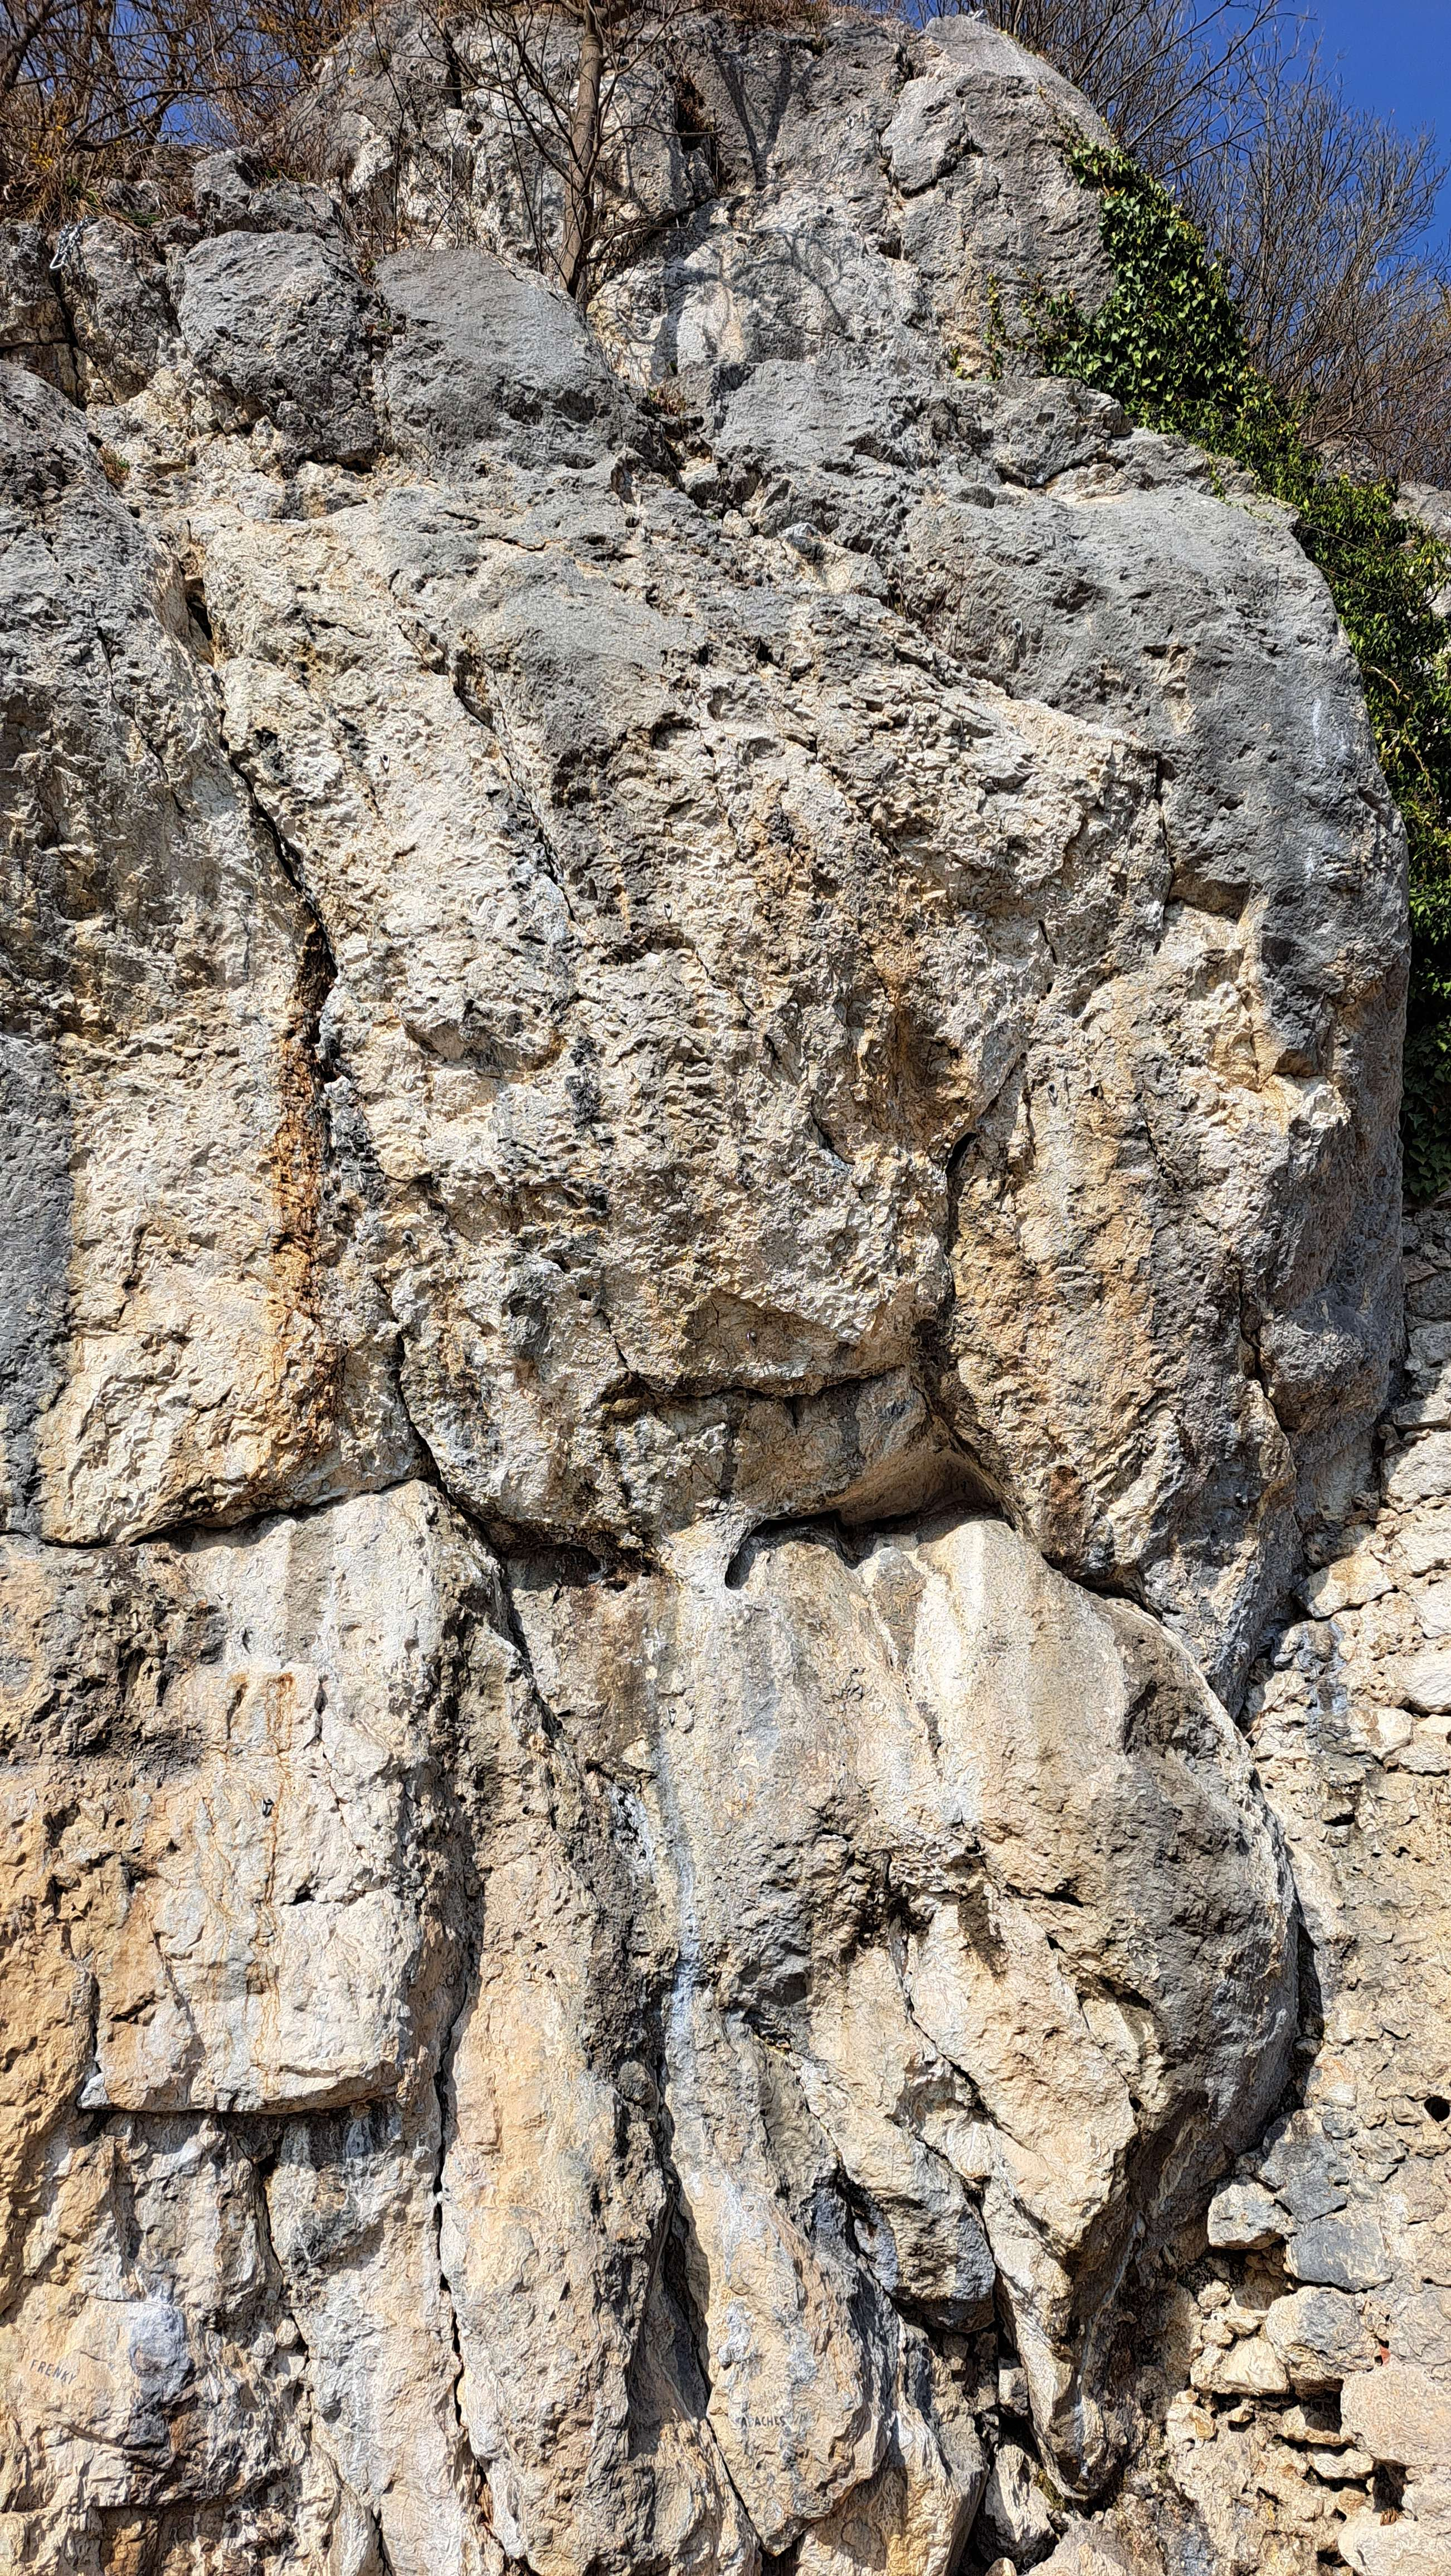
\includegraphics[width=\textwidth]{images/racunalniVid/apaches_frame.jpg}
        \caption{Slika stijene dobivena s kamere}
        \label{fig:referentna_slika_stijene}
    \end{subfigure}
    \hfill
    \begin{subfigure}[b]{0.32\textwidth}
        \centering
        \includegraphics[width=\textwidth]{images/racunalniVid/apaches_ref_photo.png}
        \caption{Referentna slika stijene}
        \label{fig:referentna_slika_linije}
    \end{subfigure}
    \hfill
    \begin{subfigure}[b]{0.32\textwidth}
        \centering
        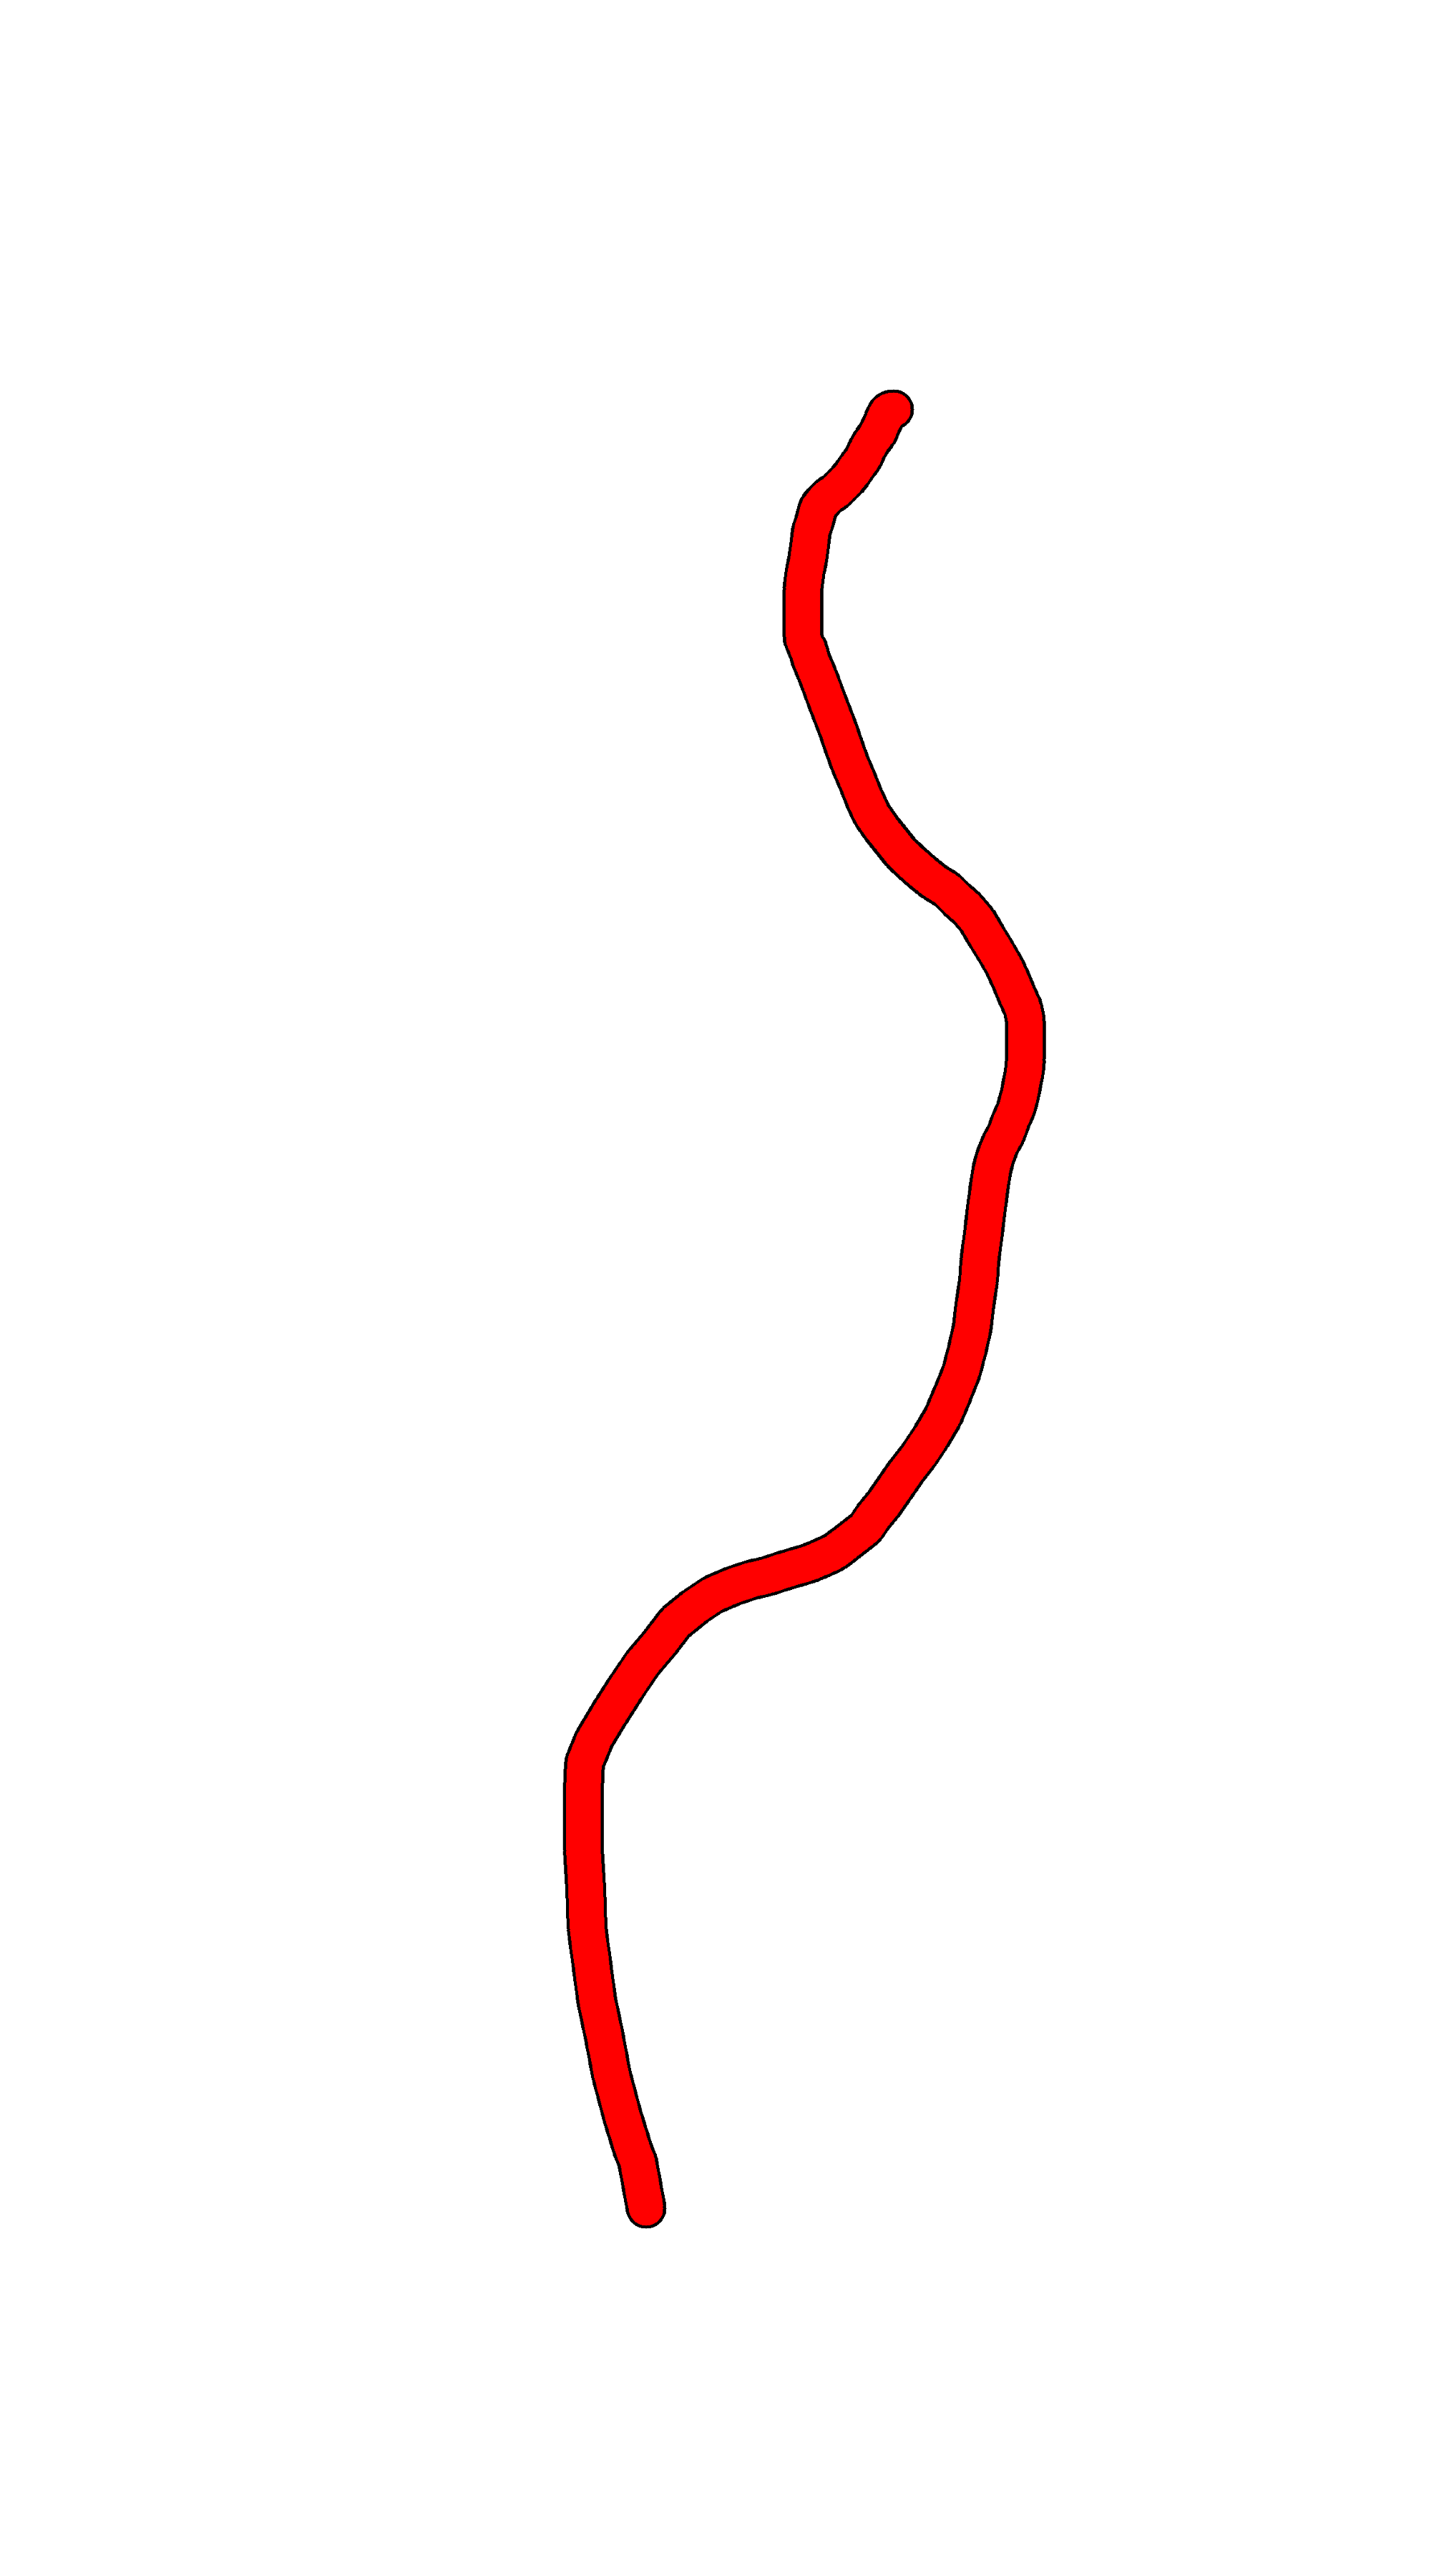
\includegraphics[width=\textwidth]{images/racunalniVid/apaches_line.png}
        \caption{Referentna slika linije smjera}
        \label{fig:slika_stijene_kamera}
    \end{subfigure}
    \caption{Tri slike potrebne za prepoznavanje penjačkog smjera}
    \label{fig:tri_kljucne_slike}
\end{figure}

Referentna slika penjačkog smjera te referentna slika linije penjačkog smjera moraju biti iste dimenzije. Proces se može se raščlaniti na sljedeće korake.
Prvi korak je detekcija i opis značajki, gdje se na referentnoj slici, unaprijed pripremljenoj slici stijene, i slici dobivenoj s kamere pronalaze ključne točke te se za svaku ključnu točku generira jedistveni numerički opis, odnosno deskriptor. Potom se uparuju značajke između slika uspoređujući deskriptore, tipično koristeći algoritam poput \textit{FLANN Matcher}. 
Te uparene značajke koriste se u trećem koraku, gdje se računa procjena geometrijske transformacije. Računa se matematički model - homografija, koja opisuje kako je slika stijene dobivene s kamera rotirana, skalirana i perspektivno izobličena u odnosu na referentnu sliku. Konačno provodi se primjena transformacije, gdje se izračunati model koristi kako bi se referentna slika linije penjačkog smjera preslikala na sliku dobivenu s kamere. Time se postiže željeni efekt vizualizacije penjačkog smjera u stvarnom vremenu.

U ovom poglavlju detaljno se obrađuju svi koraci procesa prepoznavanja penjačkog smjera, od detekcije značajki, preko uparivanja značajki do transformacije perspektive, koristeći prave slike penjačkog smjera i \textit{OpenCV} biblioteku.

\subsection{Detekcija i opis značajki (engl. feature detection and description)}

\subsection{Uparivanje značajki (engl. feature matching)}

Nakon što se odrede SIFT značajke na obije slike, potrebno je pronaći podudaranja među njima. Proces se svodi na pronalaženje parova deskriptora koji su međusobno najsličniji u visokodimenzionalnom prostoru. Postoji nekoliko metoda za mjerenje sličnosti deskriptora.

Prva metoda je korištenje \textit{brute force} algoritma. Sličnost između dva 128-dimenzionalna SIFT deskriptora mjeri se koristeći Euklidsku udaljenost formulom
\begin{equation}
    d(d_1, d_2) = \sqrt{\sum_{i=1}^{128} (d_1[i] - d_2[i])^2}
\end{equation}
gdje su $d_1$ i $d_2$ dva 128-dimenzionalna SIFT deskriptora. Manja Euklidska udaljenost predstavlja veću sličnost između deskriptora, odnosno između lokalnih struktura slike koje oni predstavljaju.
Kada bi se uparivanje izvodilo jednostavnim pronalaskom para sa minimalnom udaljenosti došlo bi do velikog broja pogrešnih podudaranja. Zbog toga se koristi algoritam zvan Loweov test omjera. Umjesto da se traži samo jedan, za svaki deskriptor s referentne slike pronalaze se dva najbliža susjeda na slici s kamere. Ako je omjer udaljenosti između najbližeg i drugog najbližeg susjeda manji od koeficijenta $t$, deskriptor se smatra valjanim podudaranjem. Ovo se može opisati formulom
\begin{equation}
    \frac{d(d_1, d_2)}{d(d_1, d_3)} < t
\end{equation}
gdje su $d_1$, $d_2$ i $d_3$ tri 128-dimenzionalna SIFT deskriptora, $d$ je Euklidska udaljenost, a $t$ je koeficijent koji se koristi za filtriranje pogrešnih podudaranja. Uobičajena vrijednost za prag $t$ je između 0.7 i 0.8. Ovaj test provjerava je li podudaranost nedvosmislena, odnosno ako je najbliži susjed znatno bliži od drugog oonda je značajka jedistvena i podudarnost je vjerojatno ispravna. Ako to nije istina onda to ukazuje na dvosmislenost i takva podudaranost se odbacuje kao nepouzdana.

Unatoč što ovaj algoritam daje dobre rezultate, njegova vremenska komplesnost ga čini nepraktičnim za rad u stvarnom vremenu. Kako bi se ubrzao proces, često se koriste algoritmi za aproksimativnu pretragu najbližih susjeda koji se oslanjaju na efikasne strukture podataka za organizaciju visokodimezionalnih vektora. Jedna od takvih struktura je \textit{k-d stablo}. K-d stablo je prostorna podatkovna struktura koja rekurzivno dijeli prostor u polovične podprostore čime postiže brzu eliminaciju velikih dijelova prostora pretrage. Unatoč njenoj efikasnosti u prostorima niske dimenzionalnosti, njena primjena u visokodimenzionalnim prostorima nije učinkovita, što je problematično za 128-dimenzionalne SIFT deskriptore. Zato je za SIFT deskriptore bolja tehnika LSH (eng. \textit{Locality-Sensitive Hashing}) koja se oslanja na hash funkcije za brzo pronalaženje sličnih vektora u visokodimenzionalnom prostoru.
U praksi se takvi algoritmi ne implementiraju ručno već se koriste gotove biblioteke koje nude bolja rješenja. Jedna od takvih biblioteka je \textit{FLANN} (eng. \textit{Fast Library for Approximate Nearest Neighbors}) koja implementira više različitih algoritama, uključujući i k-d stablo i LSH. Prednost FLANN-a je u tome što može automatski odabrati najprikladniju strukturu podataka i parametre pretrage na temelju podataka i odabranih kompromisa brzine ili preciznosti. Tim algoritmima i bibliotekama se postižu veće brzine uz minimalne gubitke u preciznosti naspram \textit{brute force} algoritma.
\subsection{Homografija i transformacija perspektive}

Rezultat procesa uparivanja značajki je skup parova odgovarajućih točaka između referentne slike i slike dobivene sa kamere, no taj skup gotovo uvijek sadrži i određeni broj pogrešnih podudaranja. Te pogreške nastanu zbog dvosmislenosti ili nesavršenosti SIFT deskriptora. Kako bi se uspostavila pouzdana geometrijska veza između dviju slika potrebno je pronaći matematički model koji opisuje transformaciju tih slika, ali na način koji je robustan na prisutnost tih pogrešnih parova. Takav model je homografija. 

Homografija je projektivna transformacija u 2D prostoru koja preslikava točke iz jedne ravnine u drugu. U ovom slučaju te ravnine su referentna slika i slika dobivena sa kamere. Homografija se može opisati 3x3 matričnom jednadžbom
\begin{equation}
    s *
    \begin{pmatrix}
        x' \\
        y' \\
        1
    \end{pmatrix}
    =
    \begin{pmatrix}
        h_1 & h_2 & h_3 \\
        h_4 & h_5 & h_6 \\
        h_7 & h_8 & h_9
    \end{pmatrix}
    \begin{pmatrix}
        x \\
        y \\
        1
    \end{pmatrix}
\end{equation}
gdje su $x$ i $y$ koordinate točke na referentnoj slici, a $x'$ i $y'$ koordinate točke na slici dobivenoj sa kamere. $s$ predstavlja faktor skale tj. $s$ je posljedica korištenja homogenih koordinata i predstavlja treću komponentu rezultirajućeg vektora prije normalizacije. Faktor $s$ osigurava da jednadžba vrijedi u projektivnom prostoru. Matrica $H$ je homografska matrica koja se sastoji od 9 koeficijenata, no $h_9$ je tipično postavljen na 1 što znači da matrica ima 8 stupnjeva slobode. Za njen izračun potrebno je poznavati barem 4 odgovarajuće točke na referentnoj i slici dobivenoj sa kamere, pod uvjetom da su točke nekolinearne.
Budući da za izračun homografije potrebno je samo četri para točaka, a iz procesa uparivanja dobije se znatno više parova, potrebno je odabrati najbolje parove na način da se također eliminira utjecaj pogrešnih podudaranosti. Za rješavanje ovog problema koristi se RANSAC (eng. \textit{Random Sample Consensus}) algoritam. RANSAC je iterativni algoritam koji se sastoji od sljedećih koraka. 
Prvo se nasumično odabire minimalni podskup podataka potreban za izračun homografije, odnosno četri para uparenih točaka. Na temelju tih nasumičnih točaka izračunava se preliminarna homografija $H$. Potom se ta preliminarna homografija testira na način da se ta matrica primjenjuje na sve ostale točke iz početnog seta podataka i određuje se udaljenost između izračunate točke i prave točke iz seta. Ako je ta udaljenost manja od predefiniranog praga onda se taj par smatra podudaranim s modelom. Cijeli ovaj postupak se ponavlja veliki broj puta. 
Na kraju se odabire matrica H koja je u jednoj od iteracija dobila najveći broj podudaranja s modelom. Korištenjem ovog algoritma osigurava se da pogrešne podudaranosti budu efikasno ignorirane jer se neće uklopiti u jedan konzistentan geometrijski model.

Kada je pronađena matrica $H$ s njom se može postići transformacija perspektive između dviju slika. Korištenjem homografije moguće je preslikati referentnu sliku linije penjačkog smjera na sliku dobivenu sa kamere koristeći OpenCV biblioteku te algoritam \textit{warpPerspective}. Kao izlaz, generira se nova slika na kojoj je sadržaj perspektivno izobličen u skladu s matricom $H$. Rezultirajuća slika transformirane linije penjačkog smjera tada se može iscrtati preko slike dobivene sa kamere. Budući da je homografija izračunata na temelju značajki sa stijene, transformirana linija će se precizno poklapati s geometrijom stijene u trenutnom pogledu kamere čime se postiže efekt proširene stvarnosti.
% \chapter{Aplikacija za prepoznavanje penjačkog smjera - Alpinity}

Nakon analize postojećih rješenja i tehnološke podloge računalnog vida, ovo poglavlje opisuje softversko rješenje razvijeno u sklopu ovog rada - sustav "Alpinity". Temeljna svrha sustava je riješiti problem idenfikacije penjačkih smjerova na terenu i omogućiti penjačku izvor informacija kako bi bolje organizirao svoje penjačke izlete. Sustav se sastoji od pozadinskog sustava te dva korisnička sučelja u obliku mobilne aplikacije za iOS platformu, koja predstavlja središnji alat za koritenje na terenu, i web aplikacije, namijenjene pregledu podataka na ostalim platformama. 

Mobilna aplikacija za iOS platformu predstavlja središnji dio sustava "Alpinity" i namijenjena je penjačima za organizaciju penjačkih izleta, ali i za korištenje na terenu. Aplikacija kombinira standardne funkcionalnosti digitalnih vodiča s mogućnosti temeljenih na proširenoj stvarnosti. Omogućuje pregled detaljnih informacija o penjalištima, sektorima i penjačkim smjerovima. Uz to, nudi i personalizirane funkcionalnosti poput vođenja dnevnika uspona i praćenja osobne statistike. 
Ključna funkcionalnost je mogućnosti korištenja kamere uređaja radi unošenja referentnih podataka o penjačkim smjerovima i vizualizacije penjačih smjerova u stvarnom vremenu pomoću tehnologije proširene stvarnosti. Web aplikacije nudi većinu funkcionalnosti mobilne aplikacije kako bi aplikacija bila dostupna svim korisnicima. Razlika između aplikacija je što u web aplikaciji nije omogućeno dodavanje referentne slike penjačkog smjera, prepoznavanje penjačkih smjerova te rad u izvanmrežnom načinu rada. 

% \section{Autentifikacija korisnika}

\subsection{Početni zaslon}

\begin{figure}[H]
  \centering
  \includegraphics[width=0.35\textwidth]{images/implementacija/first.png}
  \caption{Početni zaslon mobilne aplikacije "Alpinity"}
  \label{fig:prvi_zaslon}
\end{figure}

Prvi korak u korištenju aplikacije "Alpinity" je početni zaslon koji služi kao ulazna točka u mobilnu aplikaciju (slika~\ref{fig:prvi_zaslon}). Ovaj zaslon nudi tri opcije, prijavu, registraciju i pristup izvanmrežnom načinu rada (eng. \textit{offline mode}).

\begin{figure}[H]
  \centering
  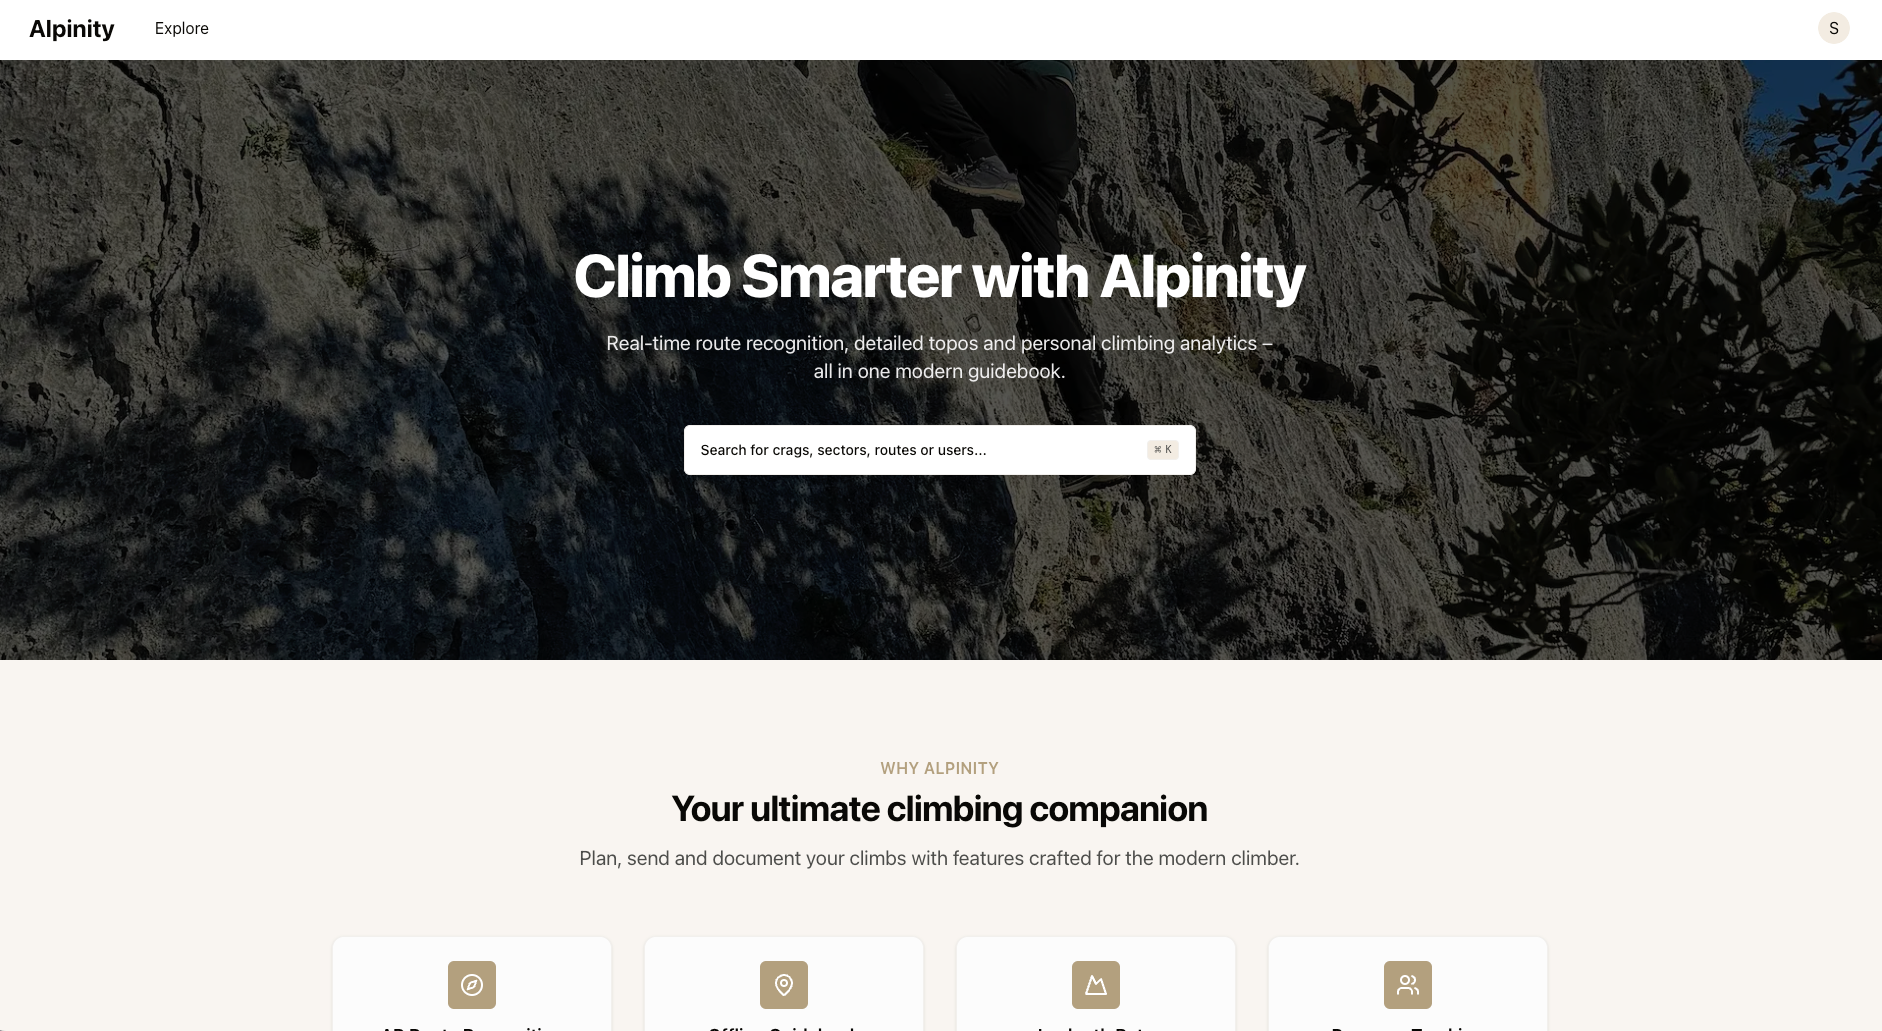
\includegraphics[width=0.9\textwidth]{images/implementacija/web/pocetni_zaslon.png}
  \caption{Početni zaslon web aplikacije "Alpinity"}
  \label{fig:prvi_zaslon_web}
\end{figure}

Na web aplikaciji, korisniku se prikazuje početni zaslon koji sadrži opis funkcionalnosti aplikacije (slika~\ref{fig:prvi_zaslon_web}). U gornjem desnom kutu nalazi se gumb za prijavu koji vodi na stranicu za prijavu iz koje se može odabrati opcija za registraciju.

\subsection{Registracija korisnika}

\begin{figure}[H]
  \centering
  \begin{subfigure}{.5\textwidth}
    \centering
    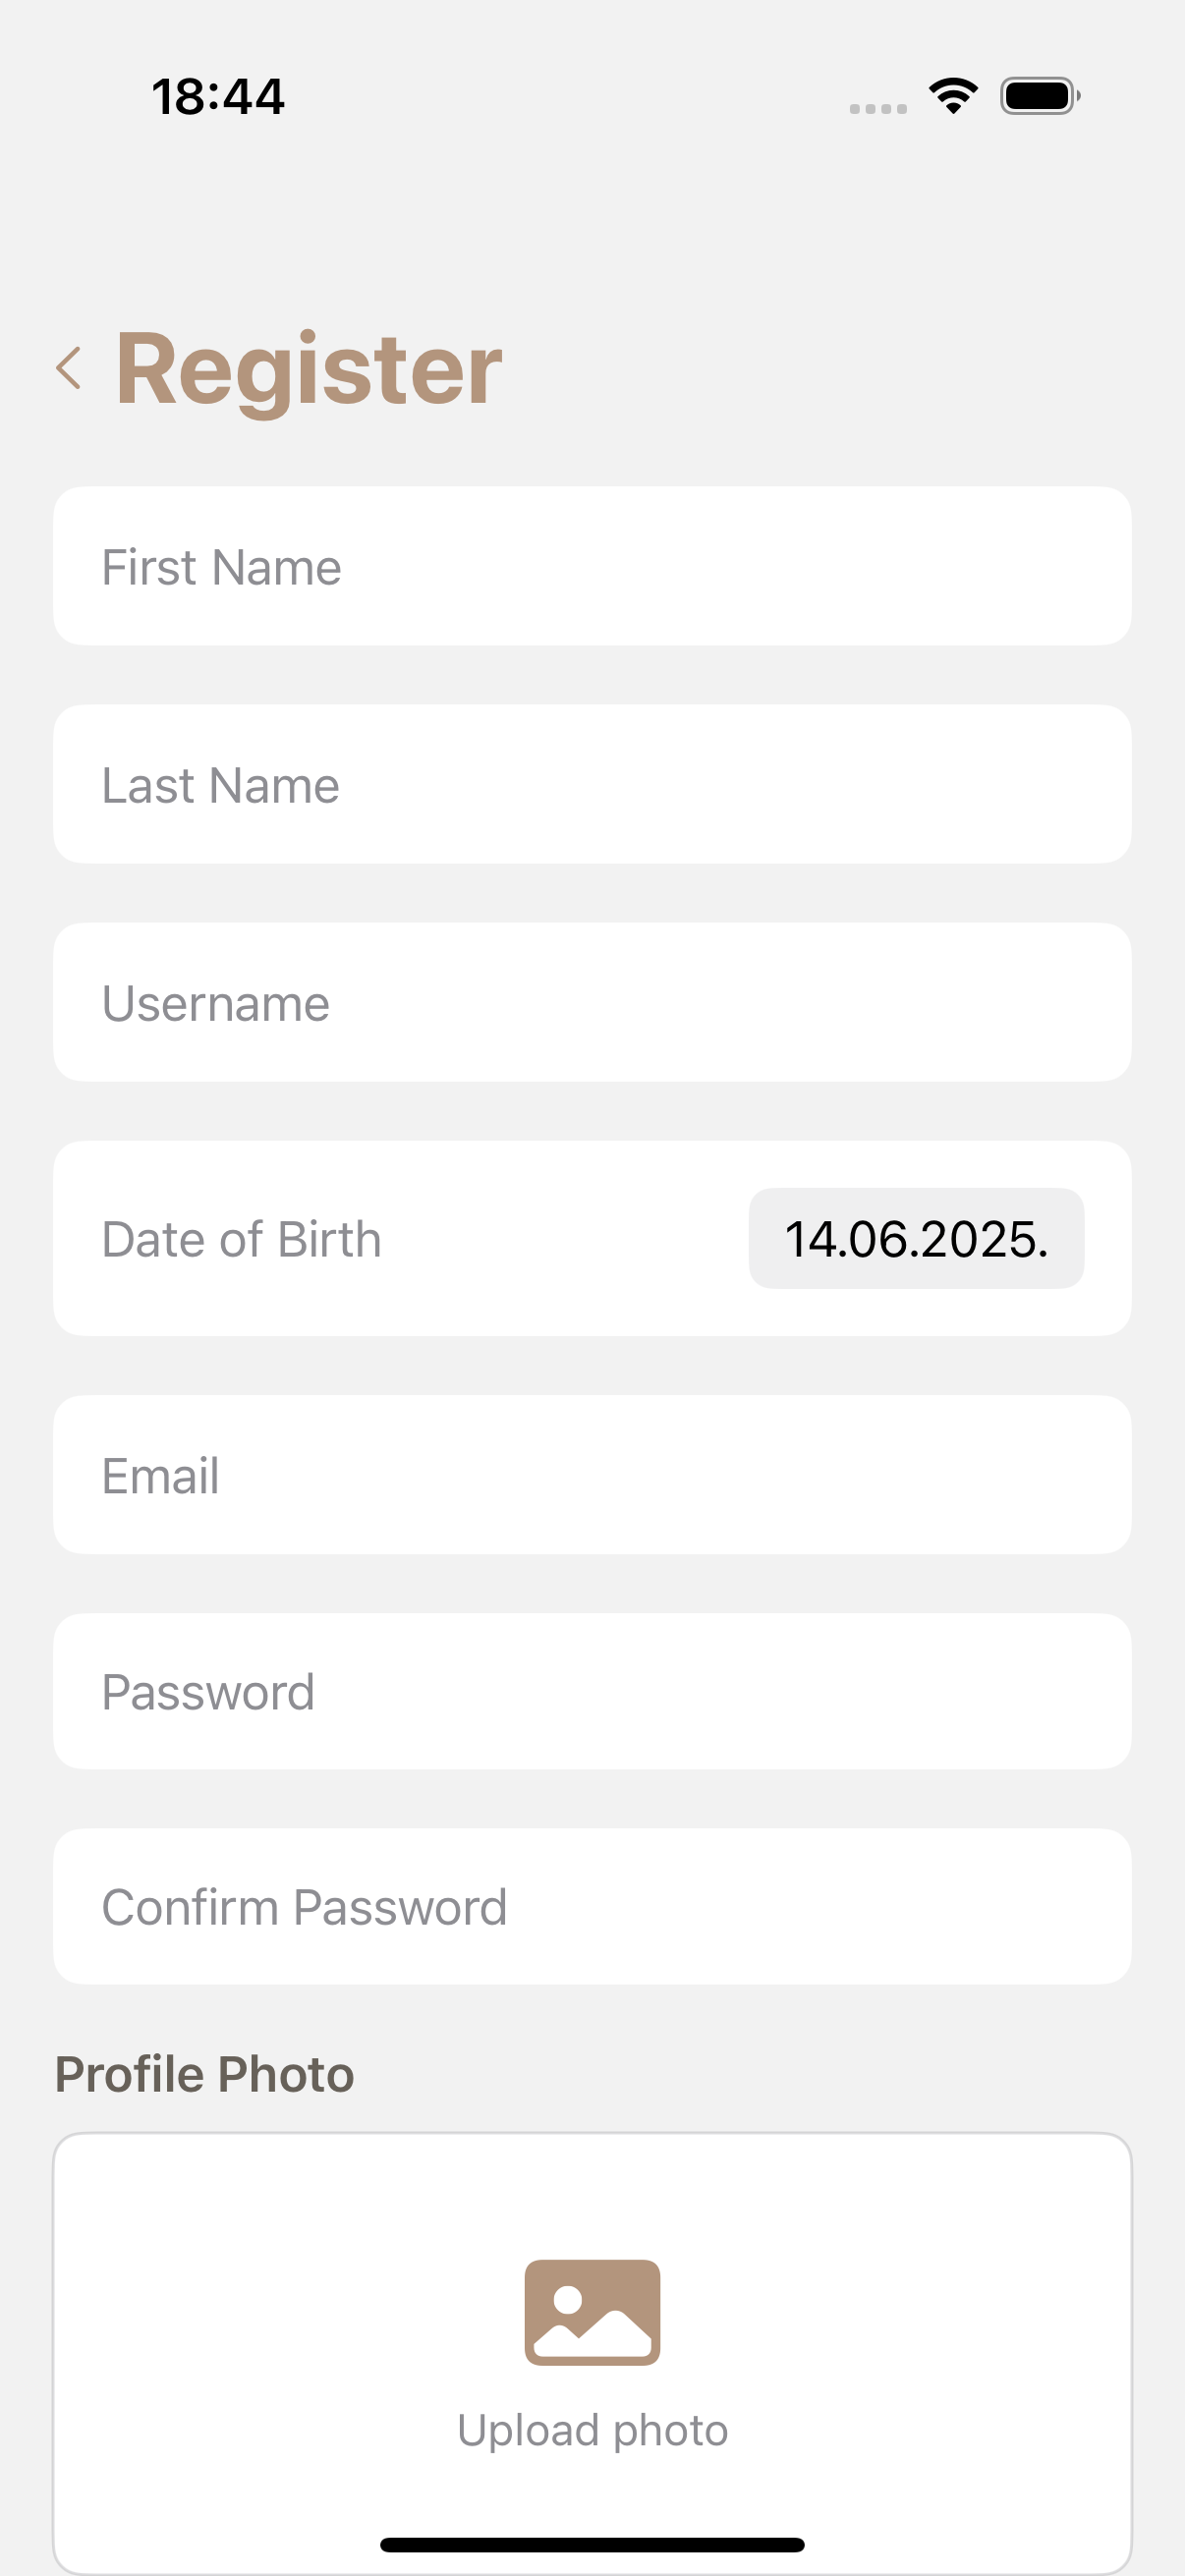
\includegraphics[width=0.7\linewidth]{images/implementacija/register.png}
    \caption{Mobilna aplikacija}
    \label{fig:registracija1}
  \end{subfigure}%
  \begin{subfigure}{.5\textwidth}
    \centering
    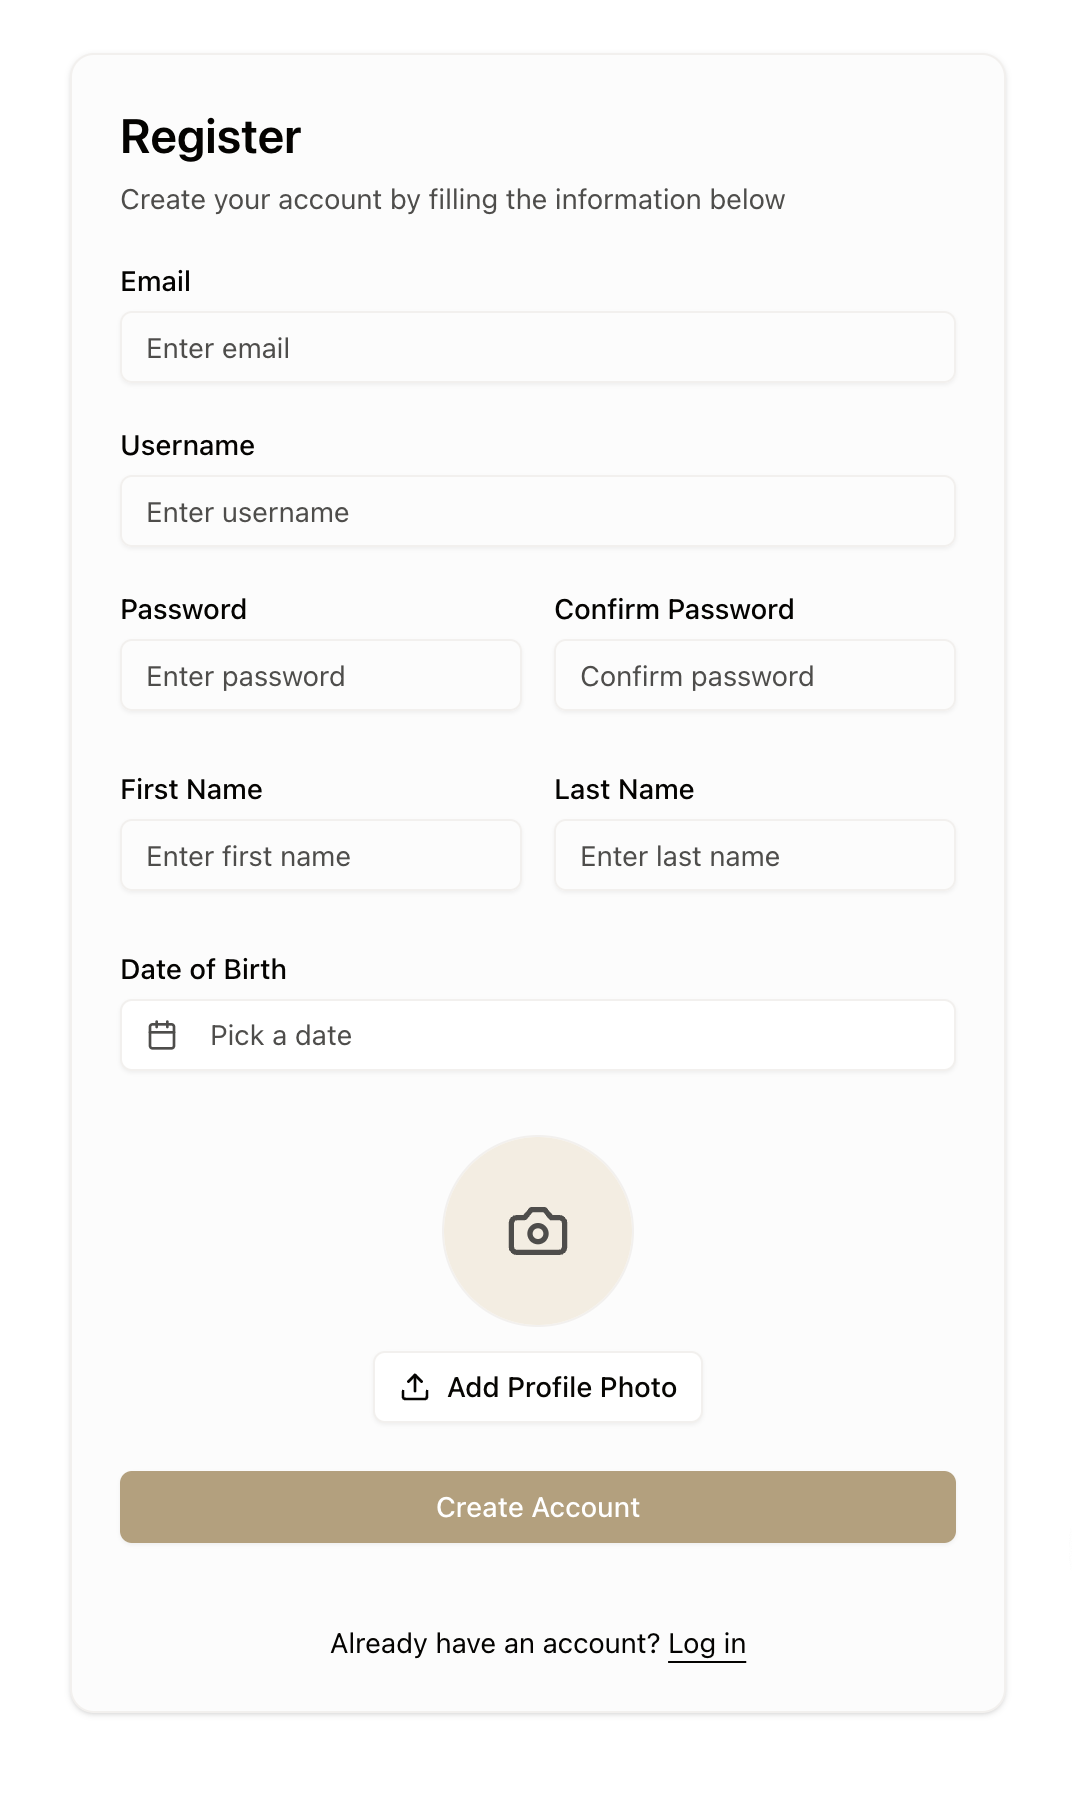
\includegraphics[width=1\linewidth]{images/implementacija/web/register.png}
    \caption{Web aplikacija}
    \label{fig:registracija2}
  \end{subfigure}
  \caption{Prikaz ekrana za registraciju korisnika u aplikaciji "Alpinity"}
  \label{fig:registracija_usporedba}
  \end{figure}


Registracija korisnika je proces kojim se stvaraju novi korisnički računi (slika~\ref{fig:registracija_usporedba}). Od korisnika se traži unos osnovnih podataka, kao što su ime, prezime, jedinstveno korisničko ime, adresa e-pošte i lozinka. Sustav također omogućuje dodavanje profilne fotografije i datuma rođenja. Proces registracije omogućuje kasnije povezivanje unesenih podataka, poput unosa u dnevnik uspona.

\subsection{Prijava korisnika}

\begin{figure}[H]
  \centering
  \begin{subfigure}{.35\textwidth}
    \centering
    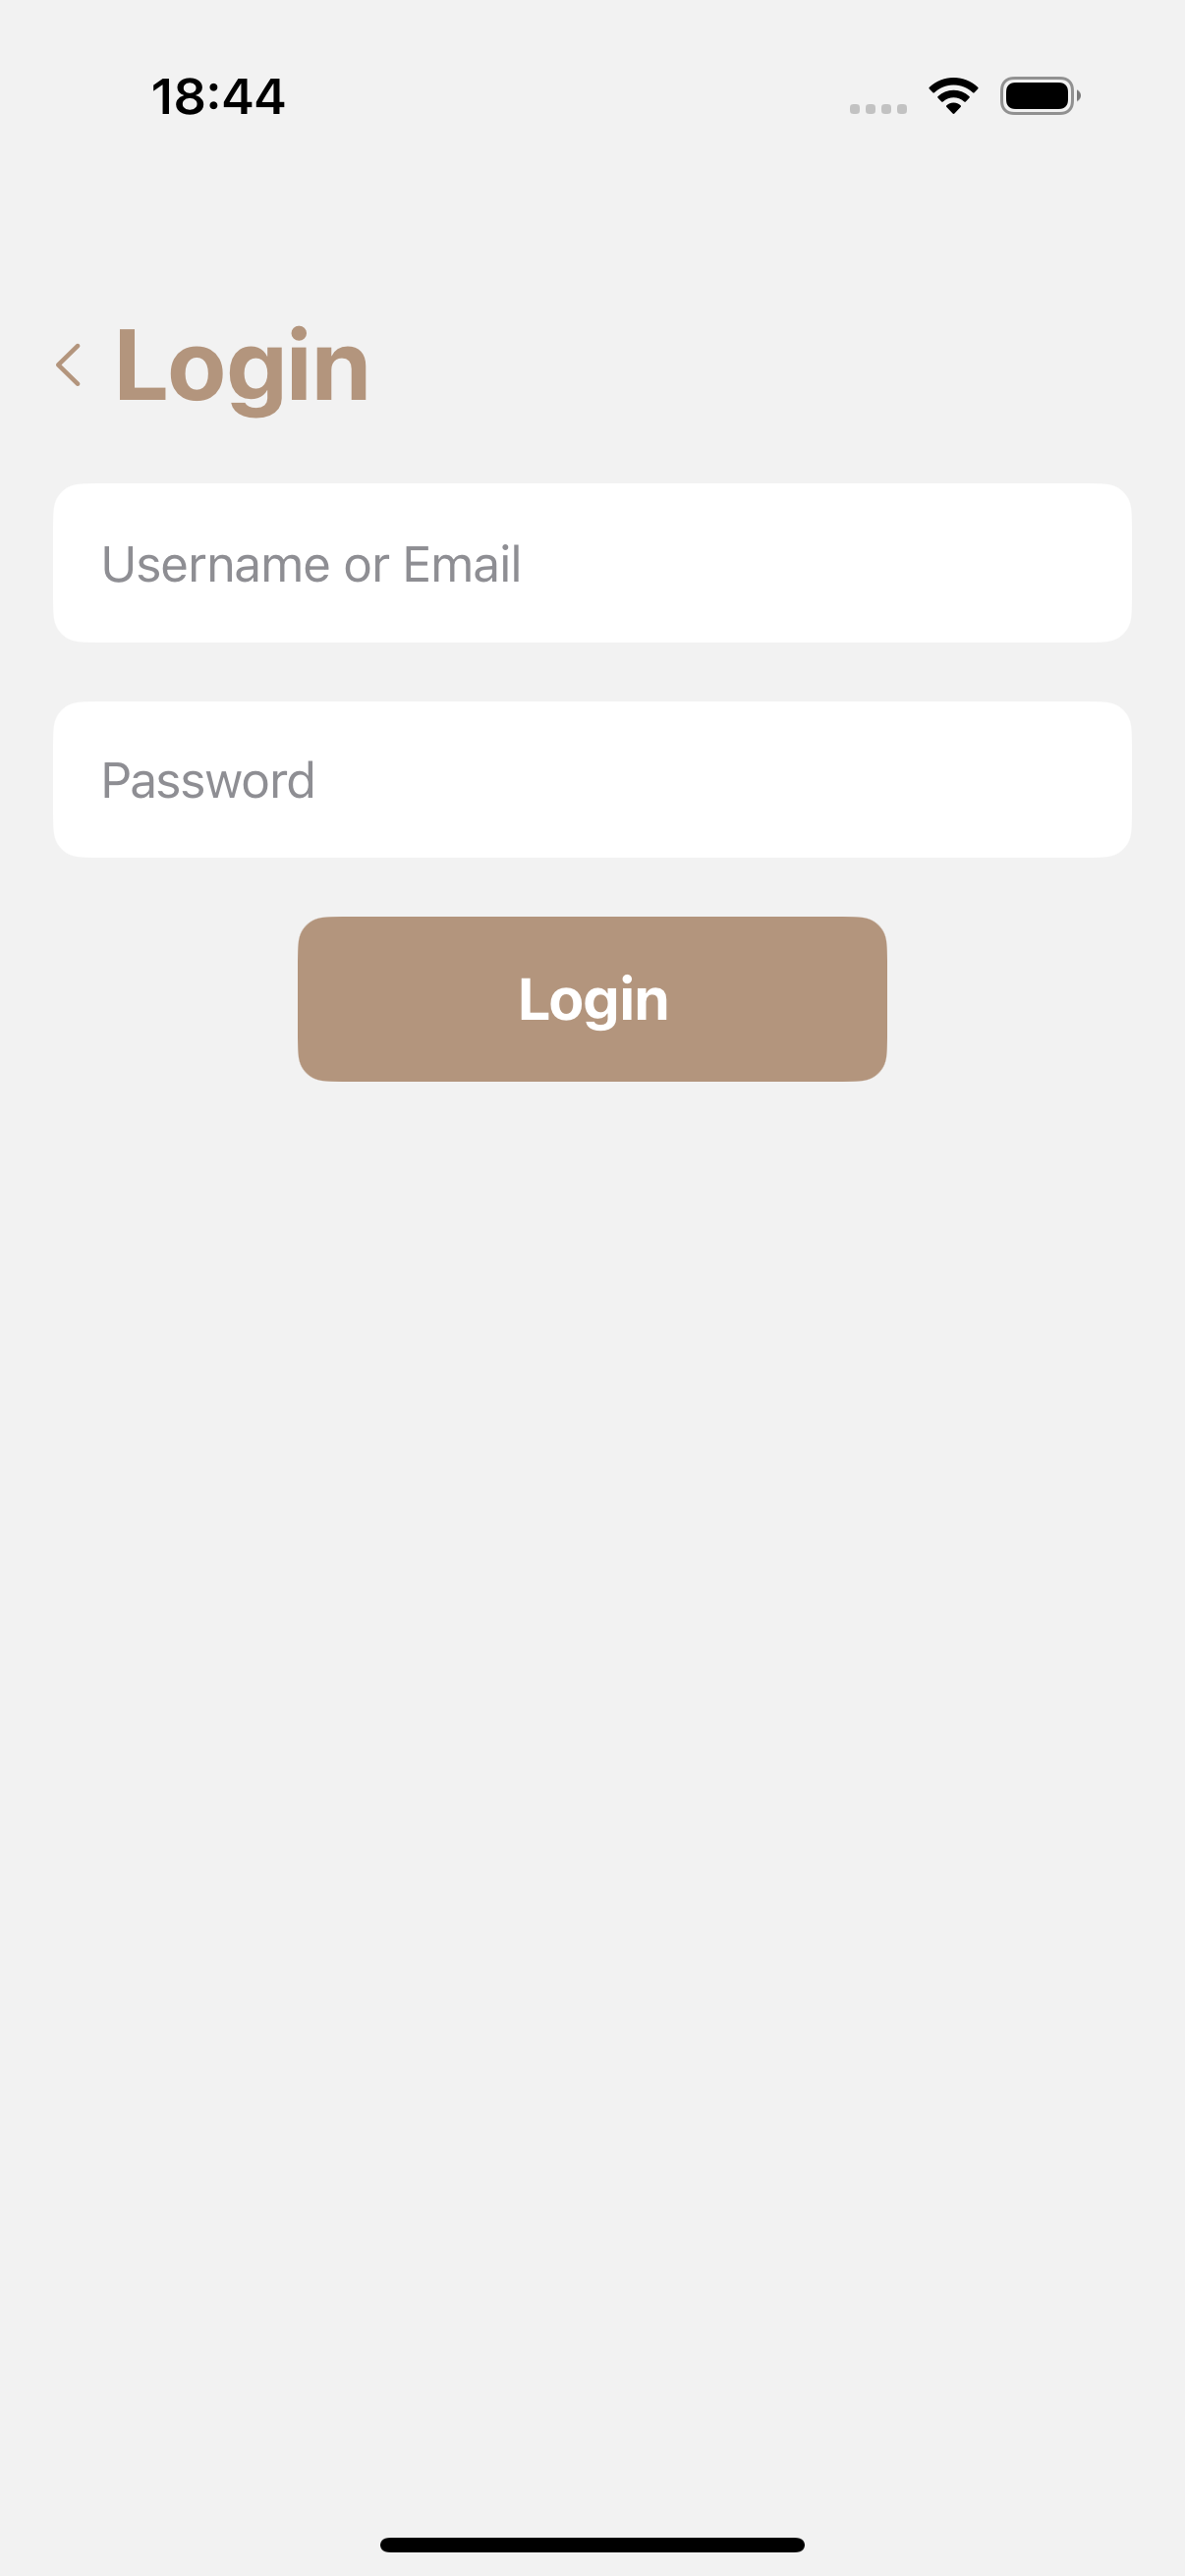
\includegraphics[width=0.9\linewidth]{images/implementacija/login.png}
    \caption{Mobilna aplikacija}
    \label{fig:prijava1}
  \end{subfigure}%
  \begin{subfigure}{.6\textwidth}
    \centering
    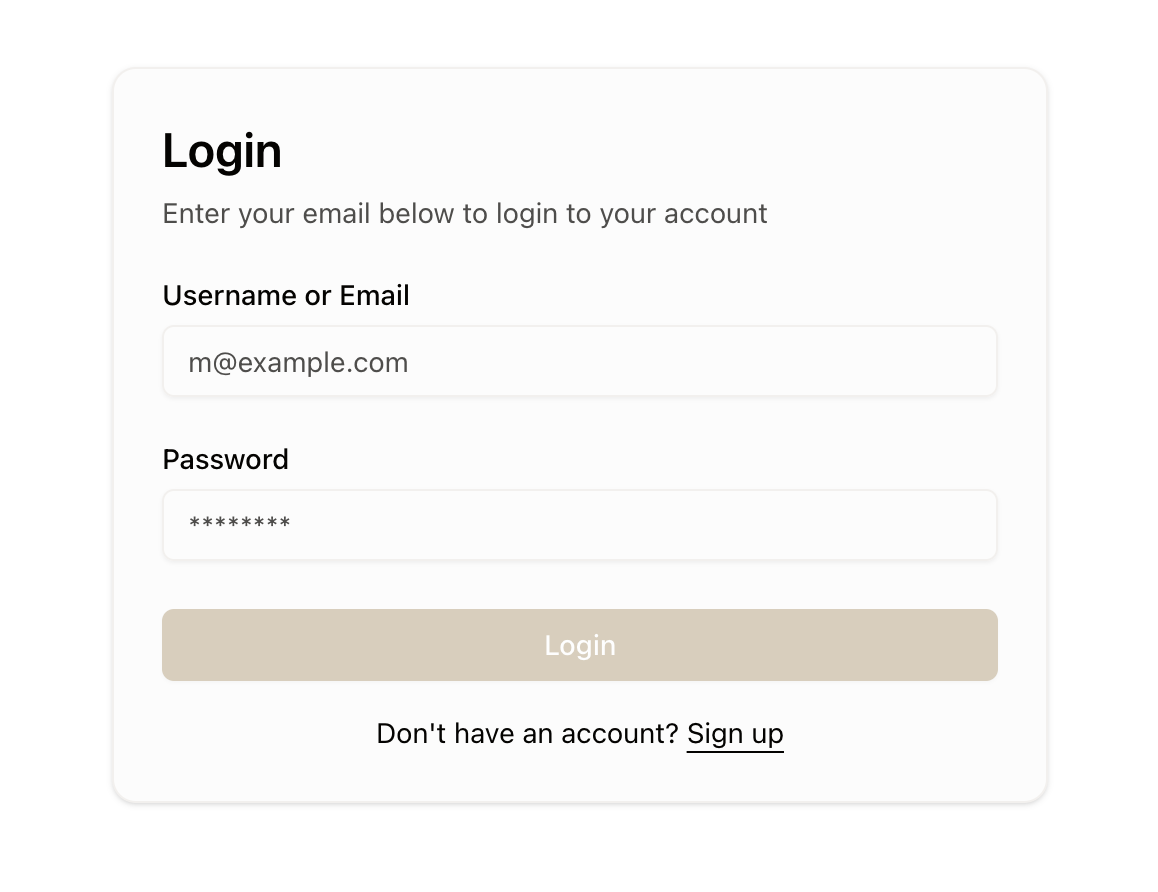
\includegraphics[width=1\linewidth]{images/implementacija/web/login.png}
    \caption{Web aplikacija}
    \label{fig:prijava2}
  \end{subfigure}
  \caption{Prikaz ekrana za prijavu korisnika u aplikaciji "Alpinity"}
  \label{fig:prijava_usporedba}
  \end{figure}

Prijava korisnika omogućuje korisniku prijavu u sustav koristeći korisničko ime ili e-mail adresu te lozinku (slika~\ref{fig:prijava_usporedba}). Nakon uspješne prijave, aplikacija pohranjuje korisničku sesiju na uređaj, čime se eliminira potreba za ponovnim unosom podataka pri sljedećem pokretanju aplikacije, te korisnik je automatski preusmjeren na početni zaslon.

Nakon prijave na web aplikaciji, korisnik se vraća na početni zaslon web aplikacije gdje sada korisnik može vidjeti mogućnosti koje su dostupne samo nakon prijave poput pretraživanja te "Istraži" (eng. \textit{Explore}) stranice.


\subsection{Odjava korisnika}

Odjava korisnika je proces kojim se korisnik odjavi iz sustava. Korisnik se može odjaviti na preko vlastitog profila, gdje se nalazi gumb "Odjava" (eng. \textit{Logout}) u izborniku. Nakon odjave, korisnik se vraća na početni zaslon za prijavu i prekida se korisnička sesija.

\subsection{Navigacija do izvanmrežnog načina rada}


Posebno važna funkcionalnost, istaknuta već na početnom zaslonu mobilne aplikacije, je izvanmrežni način rada. Ova opcija omogućuje korisnicima pristup prethodno preuzetim podacima o penjalištima i penjačkim smjerovima na udaljenim lokacijama s ograničenim ili nepostojećim internetskim signalom poput penjališta u prirodi. Time se osigurava da aplikacija bude koristna i u tim uvjetima.


% \section{Početni zaslon i glavna navigacija}

Nakon uspješne prijave na mobilnoj aplikaciji, korisnik pristupa početnom zaslonu koji je dizajniran kao personalizirana kontrolna ploča. (slika~\ref{fig:početni_zaslon})

\begin{figure}[H]
    \centering
    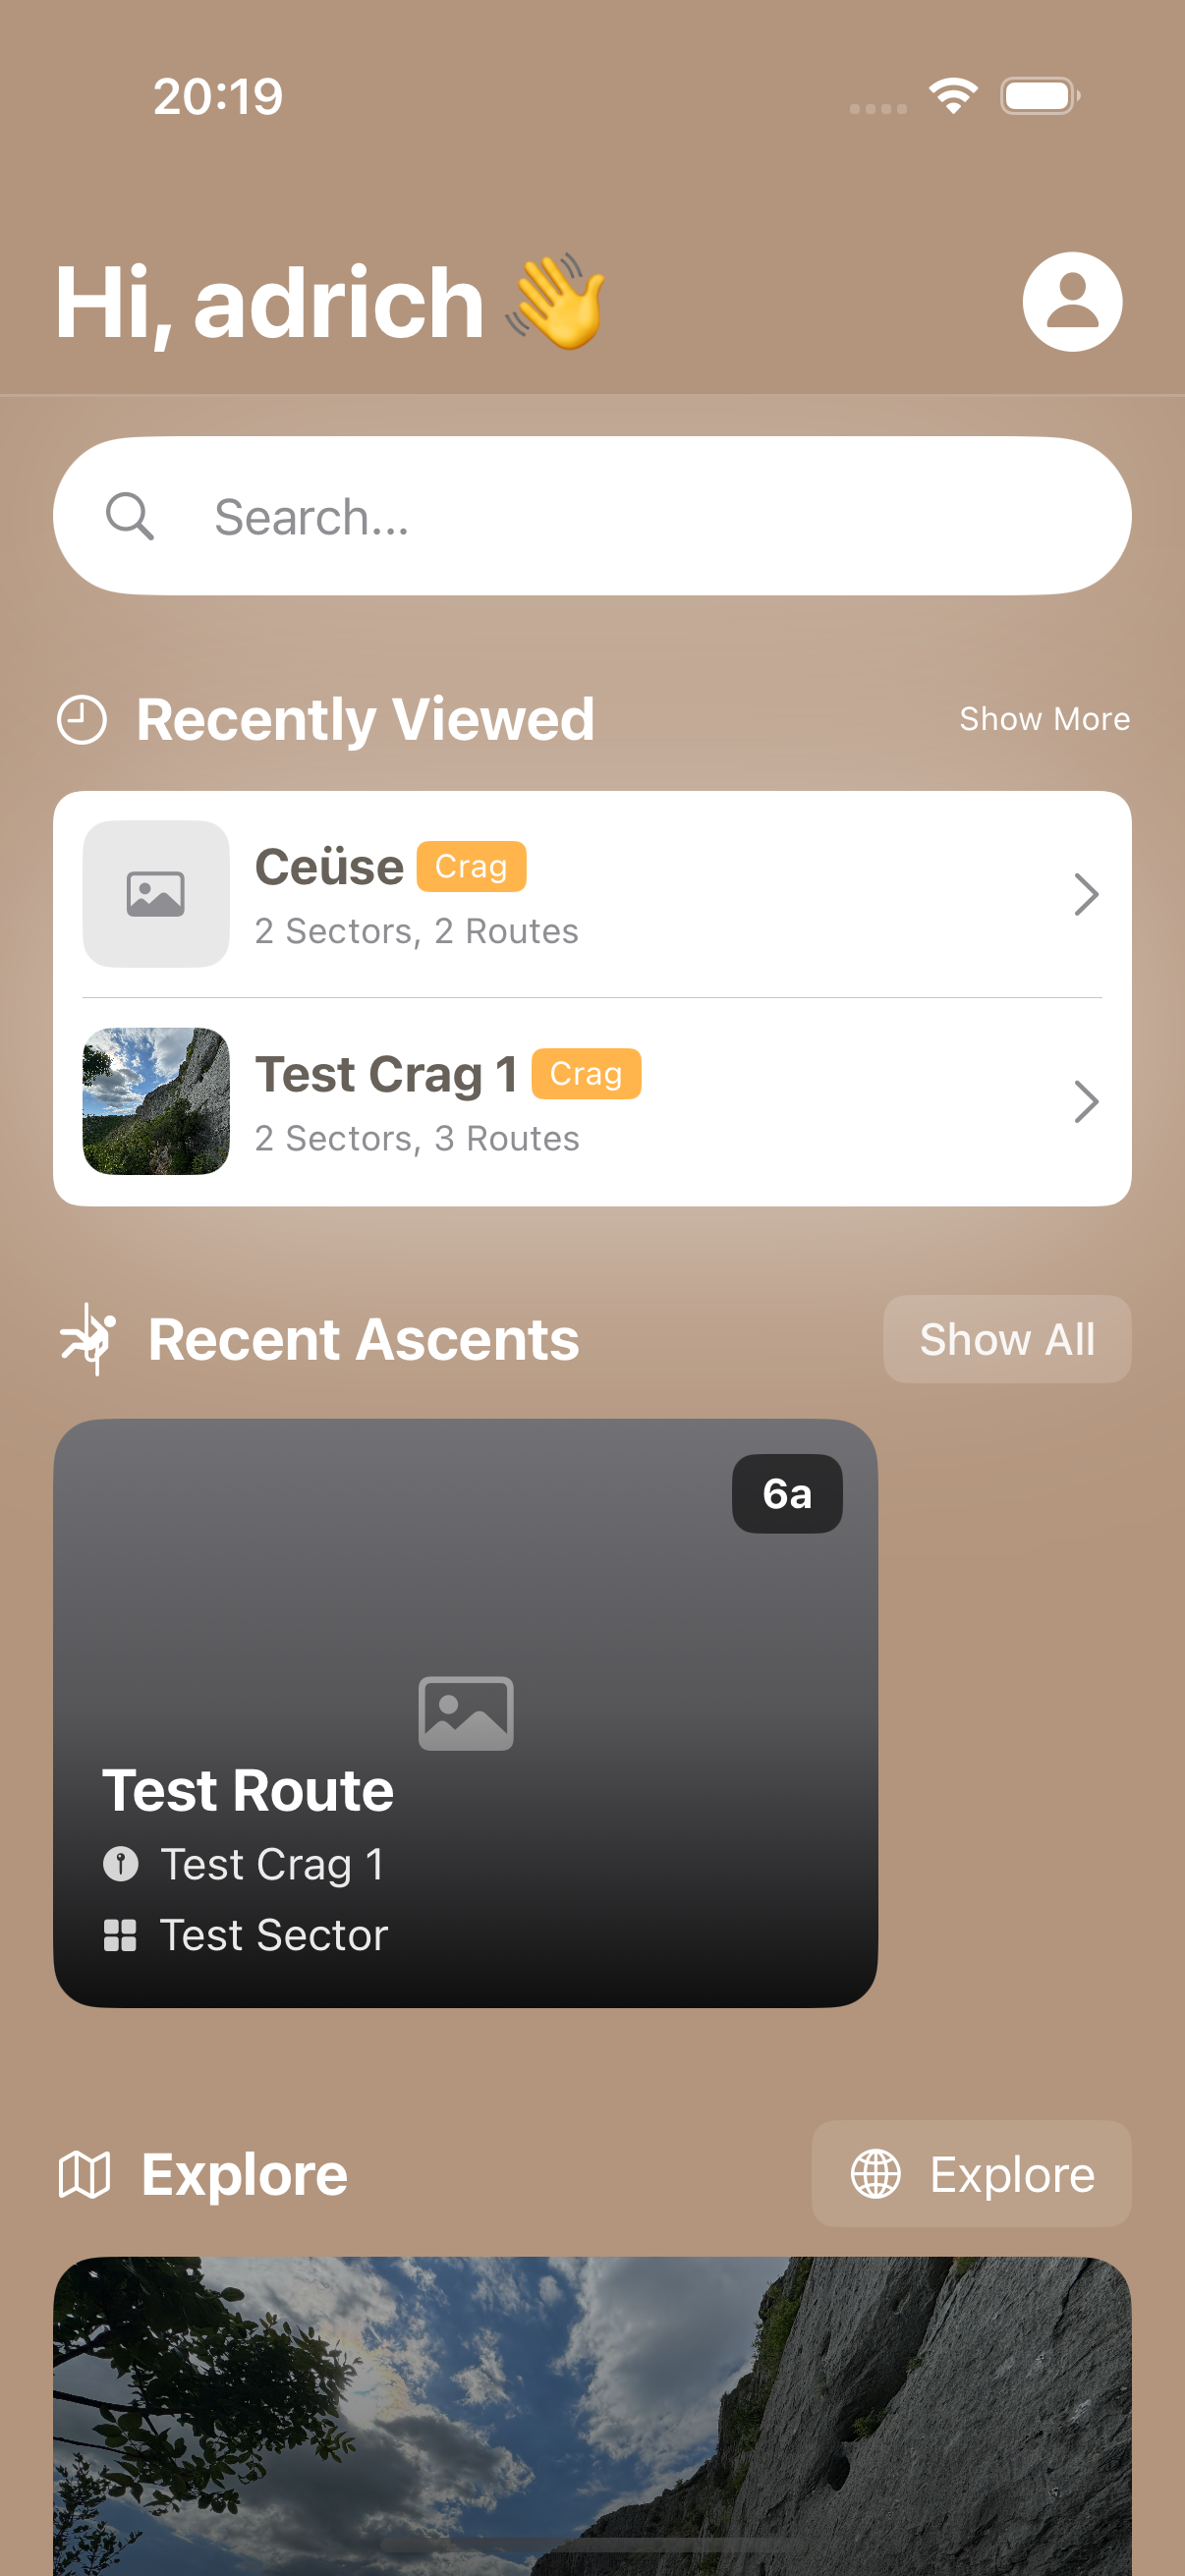
\includegraphics[width=0.35\textwidth]{images/implementacija/main_nav_1.png}
    \caption{Navigacijski zaslon aplikacije "Alpinity"}
    \label{fig:početni_zaslon}
\end{figure}

Ovaj zaslon omogućuje brzi pristup najvažnijim informacijama i funkcionalnostima. Zaslon je organiziran u nekoliko cjelina. Na vrhu zaslona nalazi se personalizirana dobrodošlica, gumb koji vodi korisnika na detalje korisničkog profila te istaknuto polje za pretraživanje koje omogućuje brzu i direktnu pretragu svih penjačkih lokacija, sektora, penjačkih smjerova i korisnika.

Sekcija "Nedavno pregledano" (eng. \textit{Recently viewed}) nudi brze poveznice na detalje penjačke lokacije, sektore, penjačke smjerove i drugih korisnika koje je korisnik nedavno pregledavao. Korisnik ima opciju "Vidi više" (eng. \textit{View more}) koja nudi korisniku prikaz više poveznica koje je posjetio.

Odmah ispod, u sekciji "Nedavni usponi" (eng. \textit{Recent ascents}) nalazi se lista najnovijih uspona korisnika zabilježenih u dnevniku uspona. Pritiskom na određeni element liste otvara se pregled detalja tog penjačkog smjera. Klikom na "Pokaži sve" (eng. \textit{Show all}) otvara se pregled vlastitog profila gdje su zapisani svi korisnikovi usponi. 

Na dnu zaslona nalazi se sekcija "Istraži" (eng. \textit{Explore}) namijenjena otkrivanju novih penjačkih lokacija pomoću prijedloga popularnih lokacija. Preporuke su određene u odnosu na prijašnje korisnikove uspone, specifično preporuke su penjačke lokacije koje se nalaze u blizini lokacija koje je korisnik nedavno posjetio. Klikom na određenu penjačku lokaciju u listi odlazi se na pregled detalja te lokacije. Pritiskom na gumb "Istraži" (eng. \textit{Explore}) otvara se pregled sa geografskom kartom sa svim penjačkim lokacijama.

Na web aplikaciji ne postoji ekvivalent za početni zaslon mobilne aplikacije, već poveznice na nedavno pregledane entitete nalaze se u sklopu pretraživanja. Nedavni usponi su dostupni u sklopu stranice korisničkog profila, a "Istraži" sekcija je pretvorena u zasebnu stranicu koja sadrži geografsku kartu sa penjačkim lokacijama i prijedlozima popularnih lokacija (slika~\ref{fig:istrazivanje_web}).

\begin{figure}[H]
    \centering
    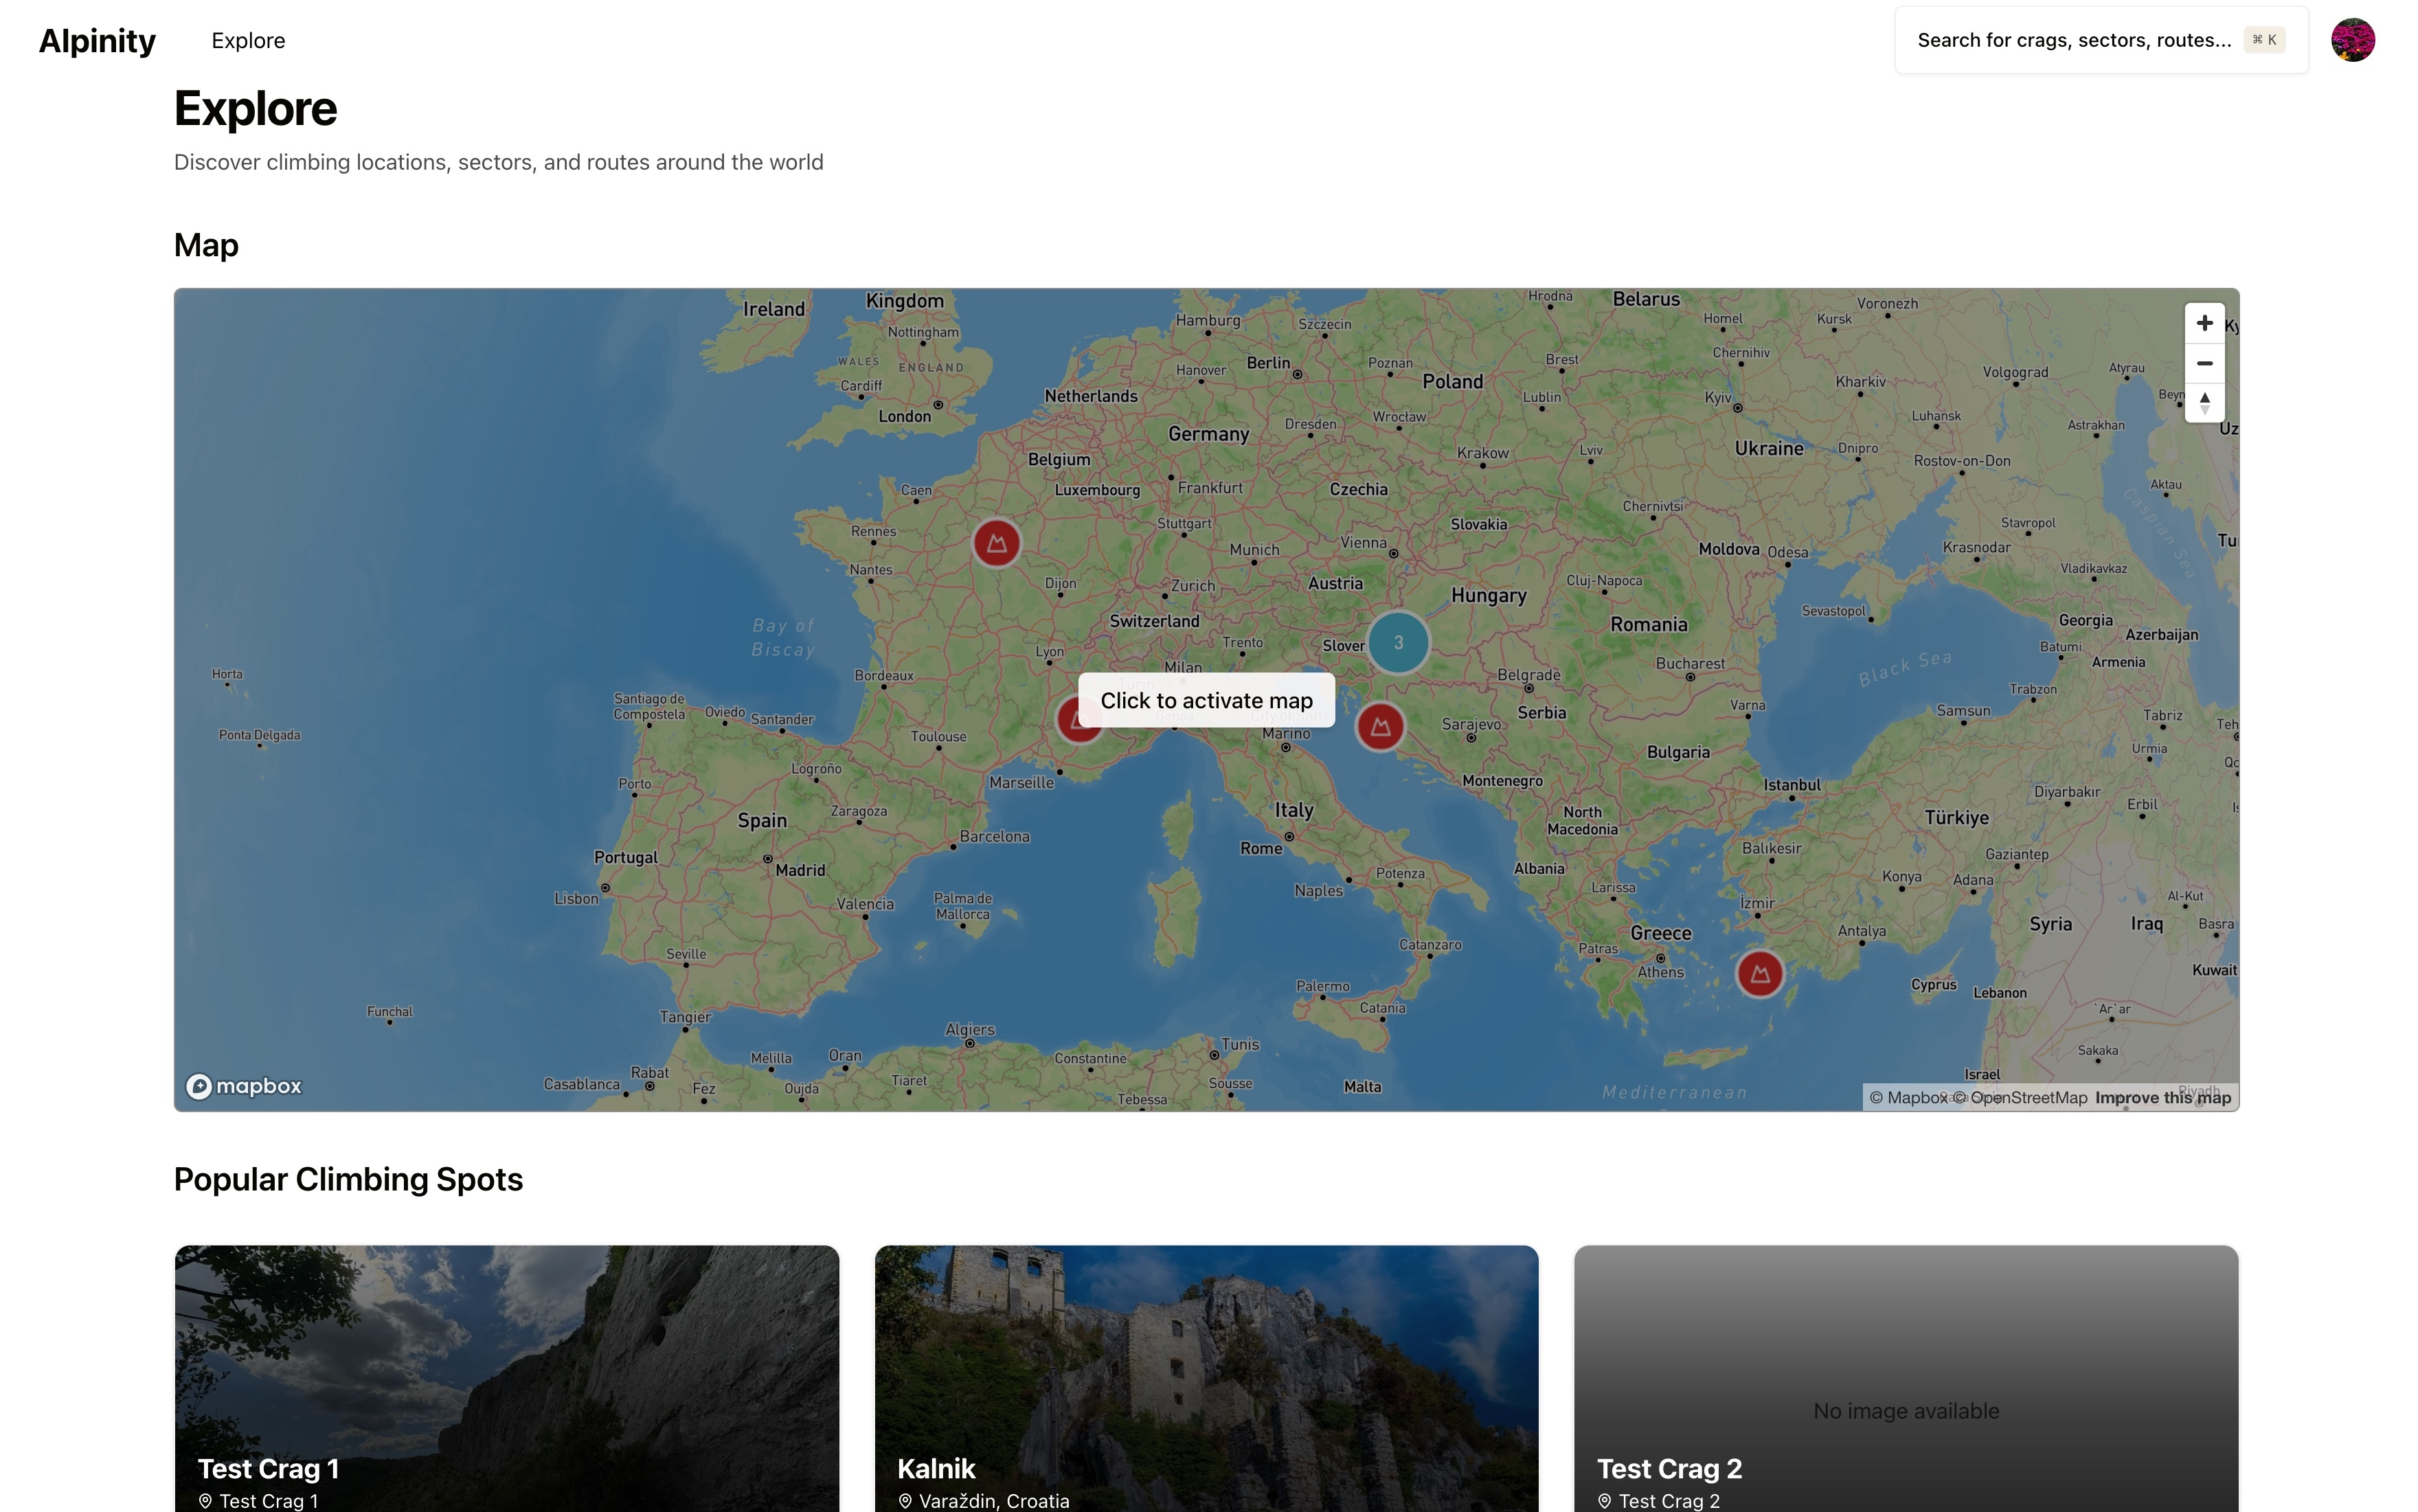
\includegraphics[width=0.9\textwidth]{images/implementacija/web/explore.jpeg}
    \caption{"Istraži" stranica web aplikacije "Alpinity"}
    \label{fig:istrazivanje_web}
\end{figure}
% \section{Geografska karta penjačkih lokacija}

Kako bi se korisnicima olakšala prostorna orijentacija, aplikacije integriraju interaktivnu geografsku kartu. Ova funkcionalnost omogućuje vizualno istraživanje penjačkih lokacija na globalnoj razini kao i detaljnu navigaciju unutar pojedinog penjališta.

\begin{figure}[H]
    \centering
    \begin{subfigure}[b]{\textwidth}
        \centering
        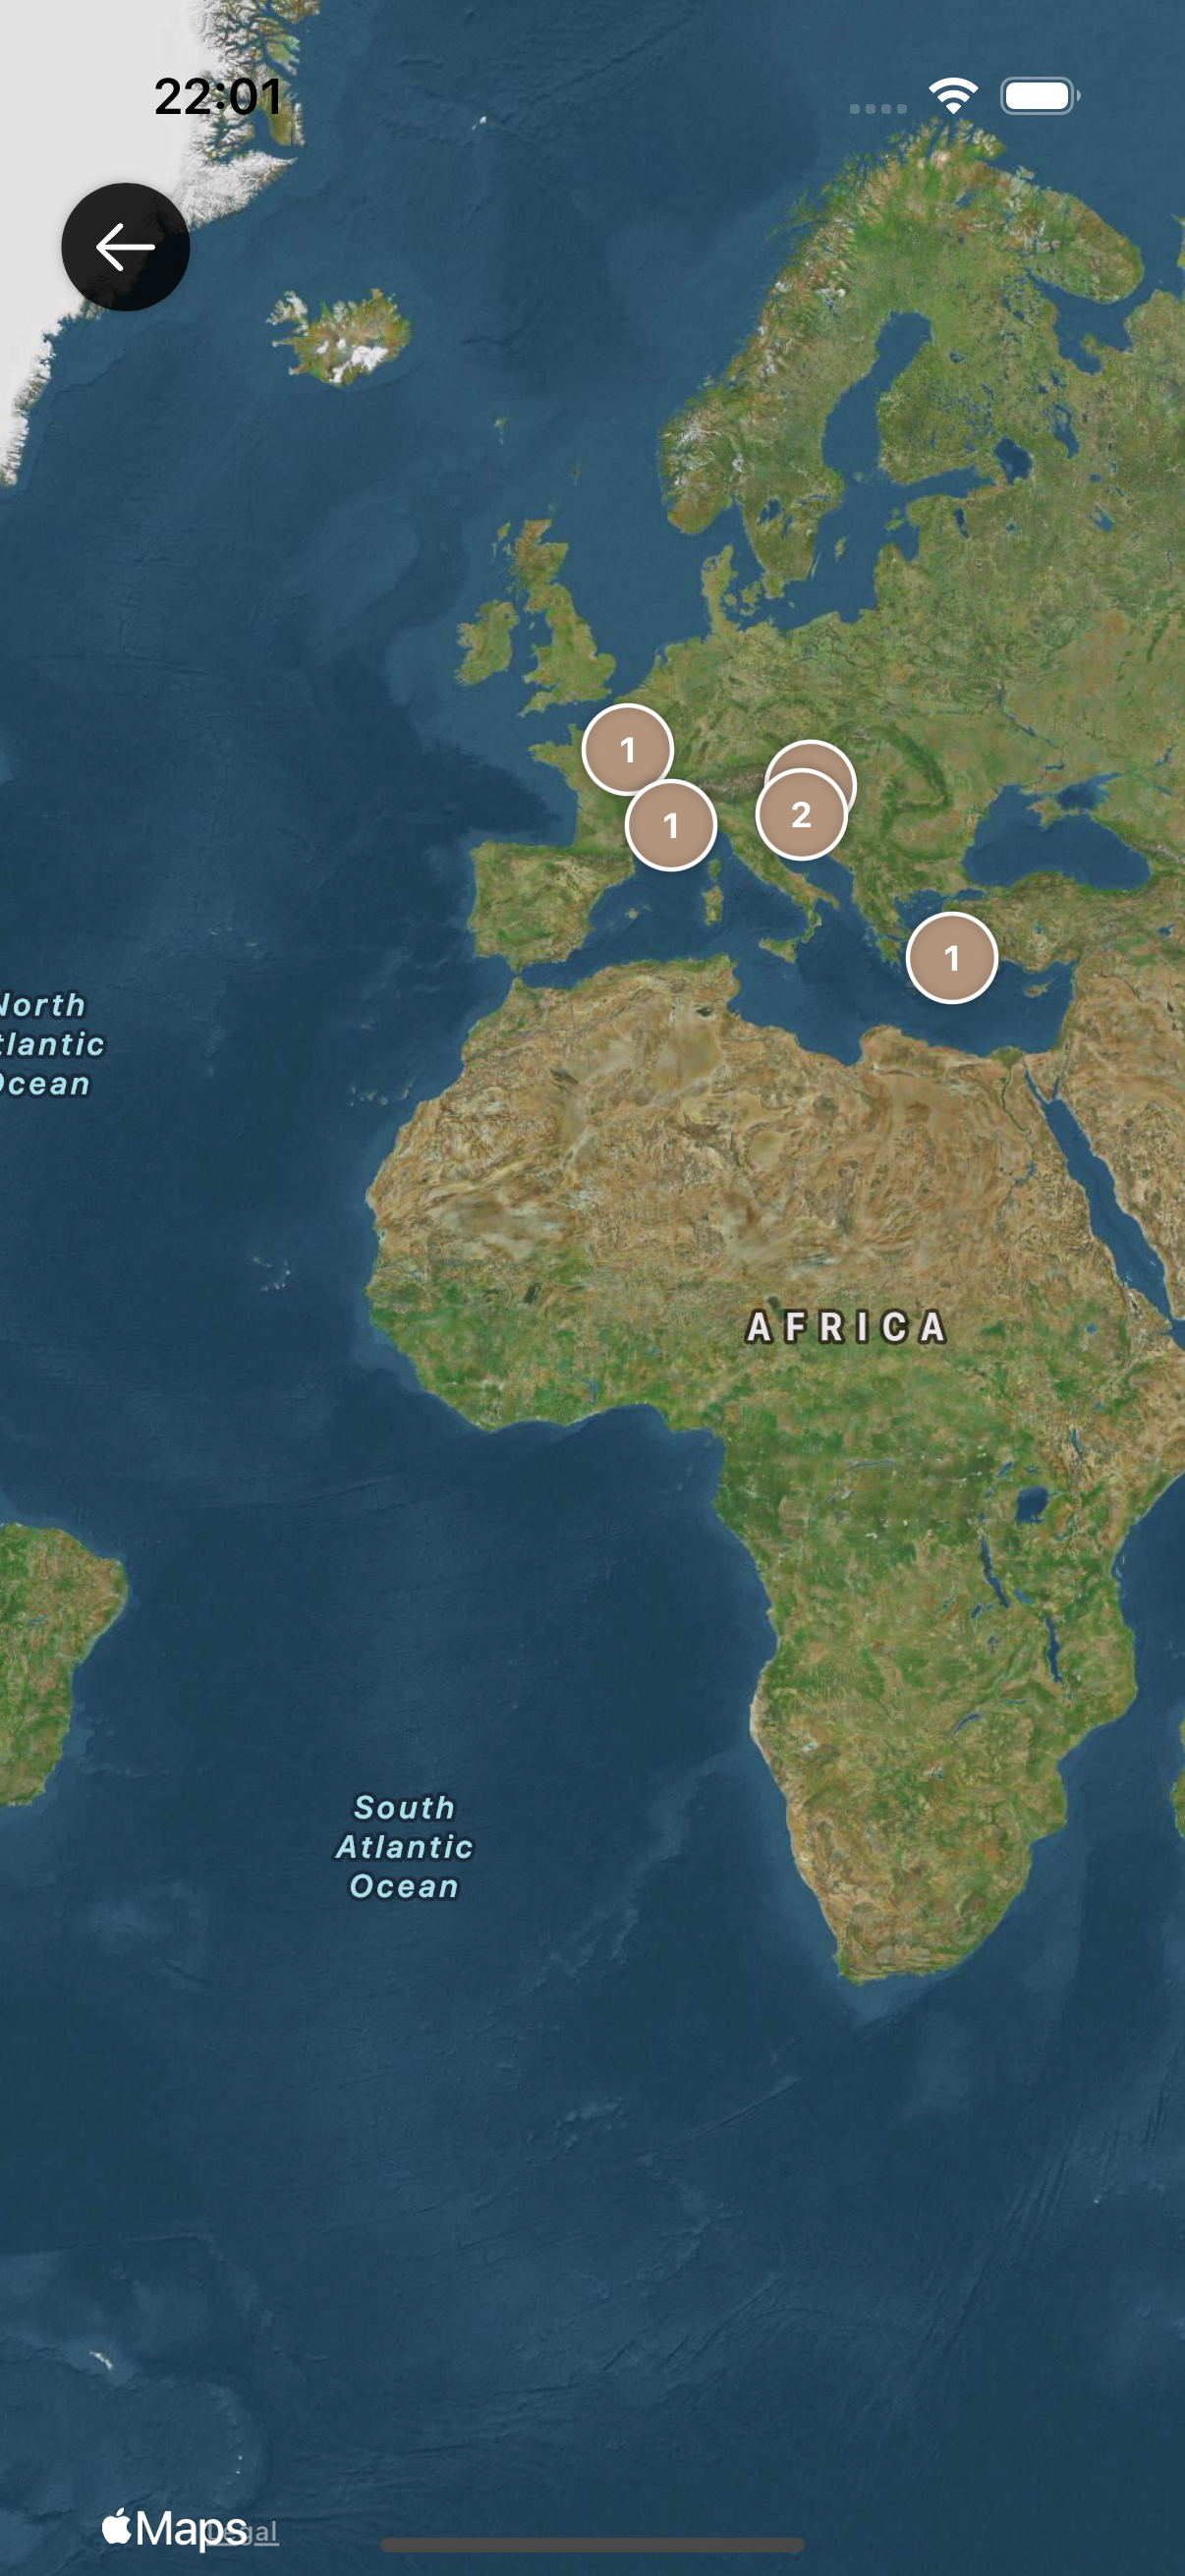
\includegraphics[width=0.3\textwidth]{images/implementacija/geo_karta.png}
        \caption{Mobilna aplikacija}
        \label{fig:geografska_karta_mob}
    \end{subfigure}
    \hfill
    \begin{subfigure}[b]{\textwidth}
        \centering
        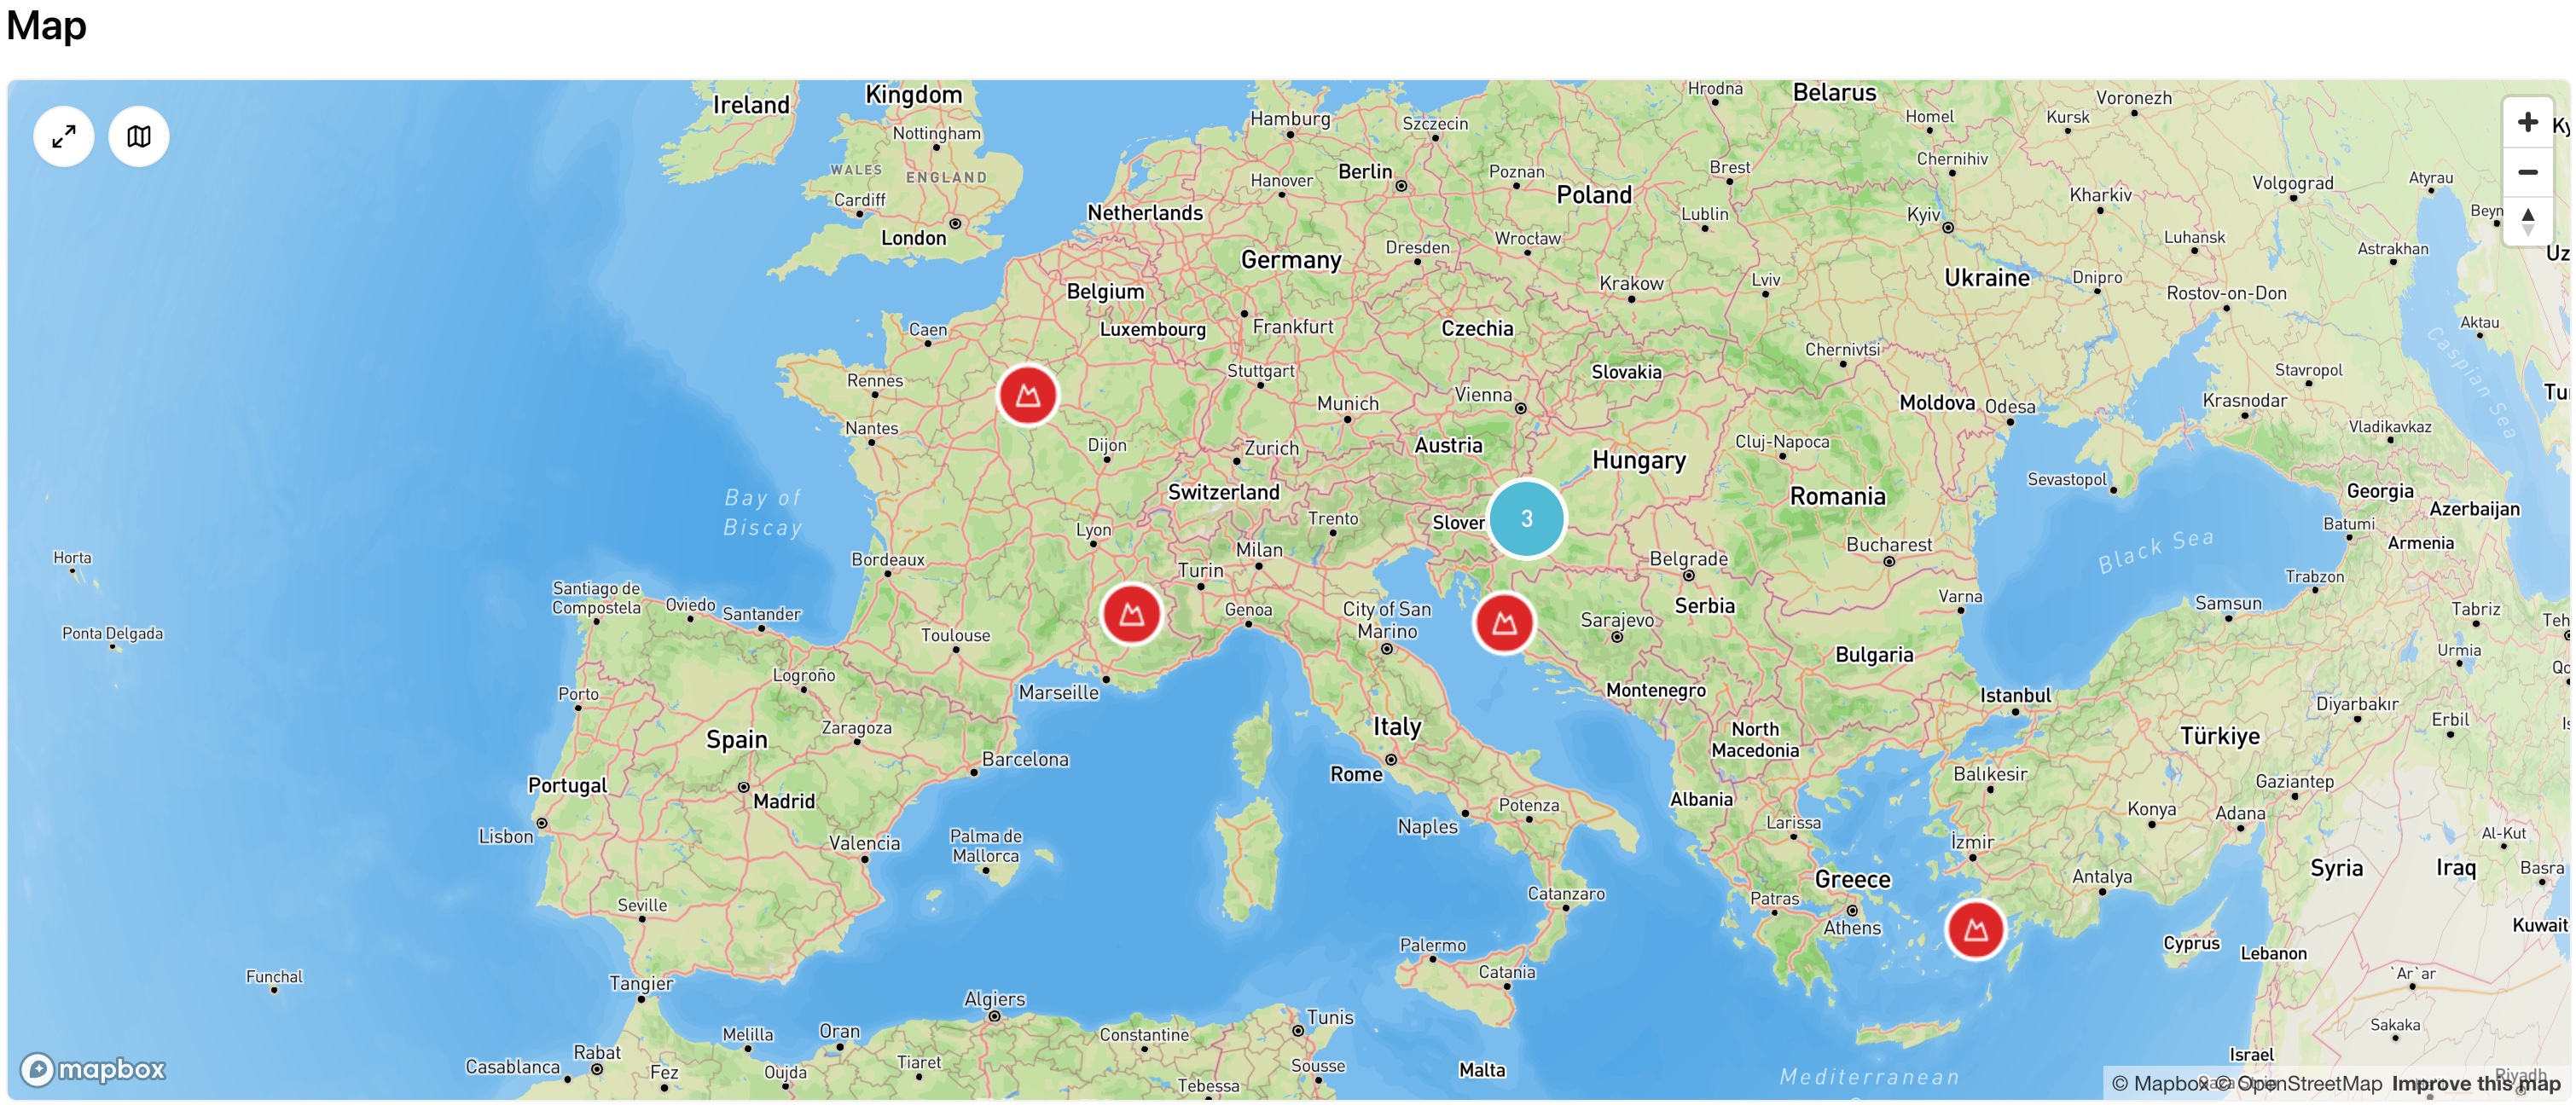
\includegraphics[width=0.9\textwidth]{images/implementacija/web/map_clusters.jpeg}
        \caption{Web aplikacija}
        \label{fig:geografska_karta_web}
    \end{subfigure}
    \caption{Geografska karta penjačkih lokacija s prikazom grupiranih oznaka}
    \label{fig:geografska_karta_sidebyside}
\end{figure}

Pristupom karti korisniku se prikazuje karta svijeta s grupiranim oznakama (eng. \textit{clusters}) koje indiciraju broj dostupnih penjališta na određenom području. Grupirane oznake omogućuju pregled prikaza na visokoj razini, ali bez pretrpanosti informacijama. Približavanjem karte, grupirane oznake se razdvajaju, otkrivajući pojedinačne lokacije penjališta.

\begin{figure}[H]
    \centering
    \begin{subfigure}[b]{\textwidth}
        \centering
        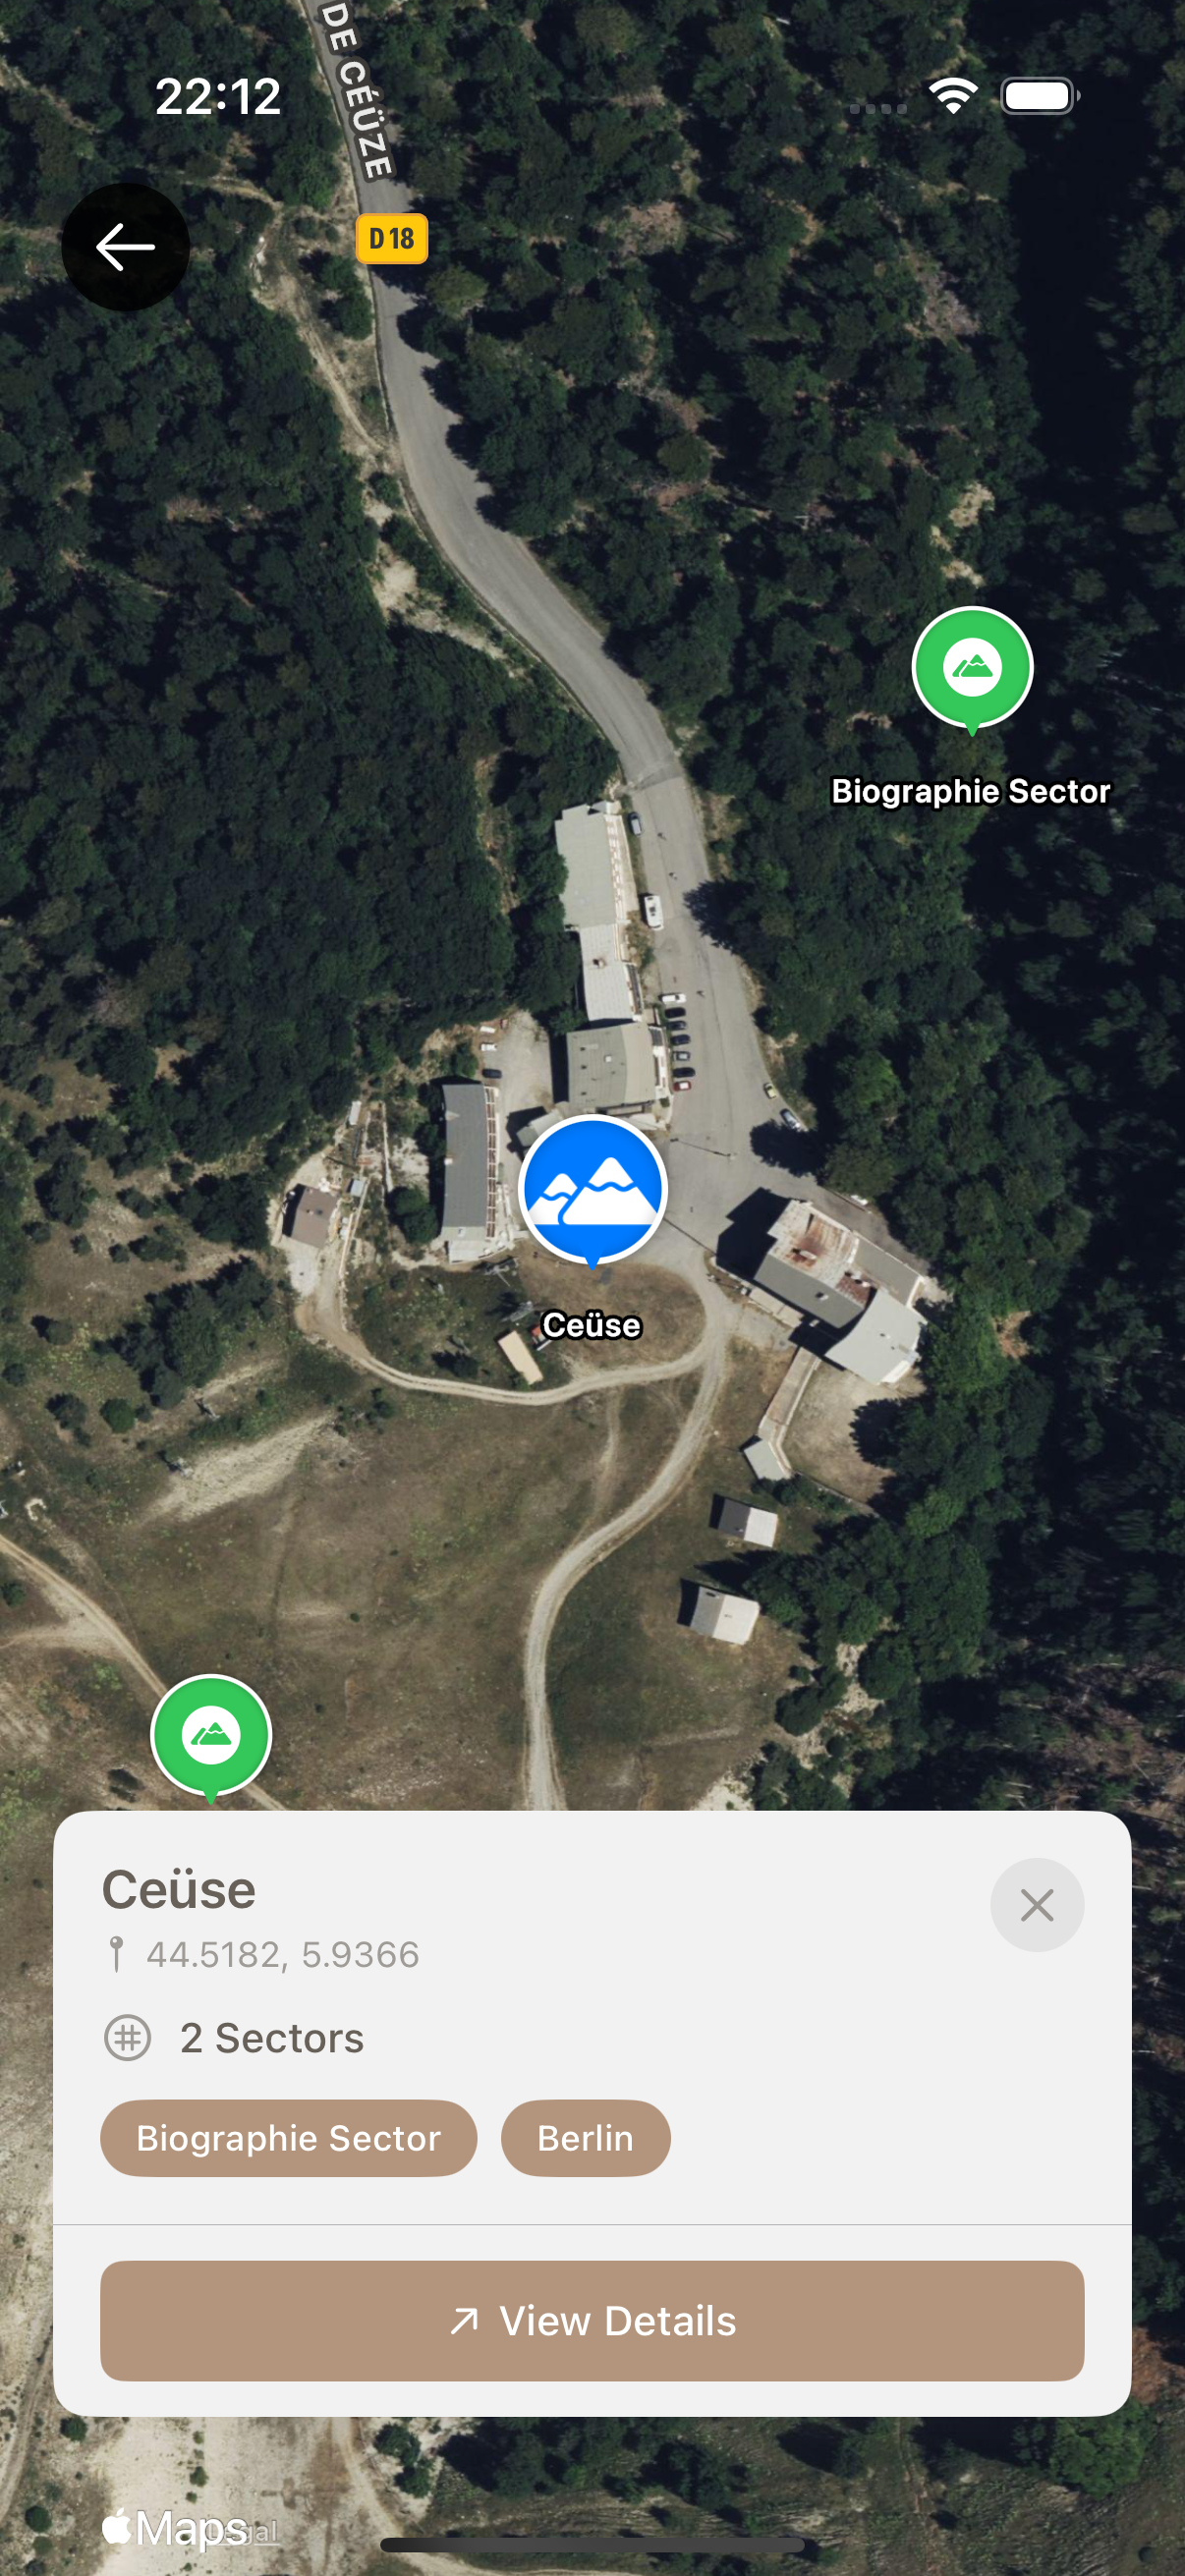
\includegraphics[width=0.3\textwidth]{images/implementacija/geo_karta_ceuse.png}
        \caption{Mobilna aplikacija}
        \label{fig:geografska_karta_ceuse_mob}
    \end{subfigure}
    \hfill
    \begin{subfigure}[b]{\textwidth}
        \centering
        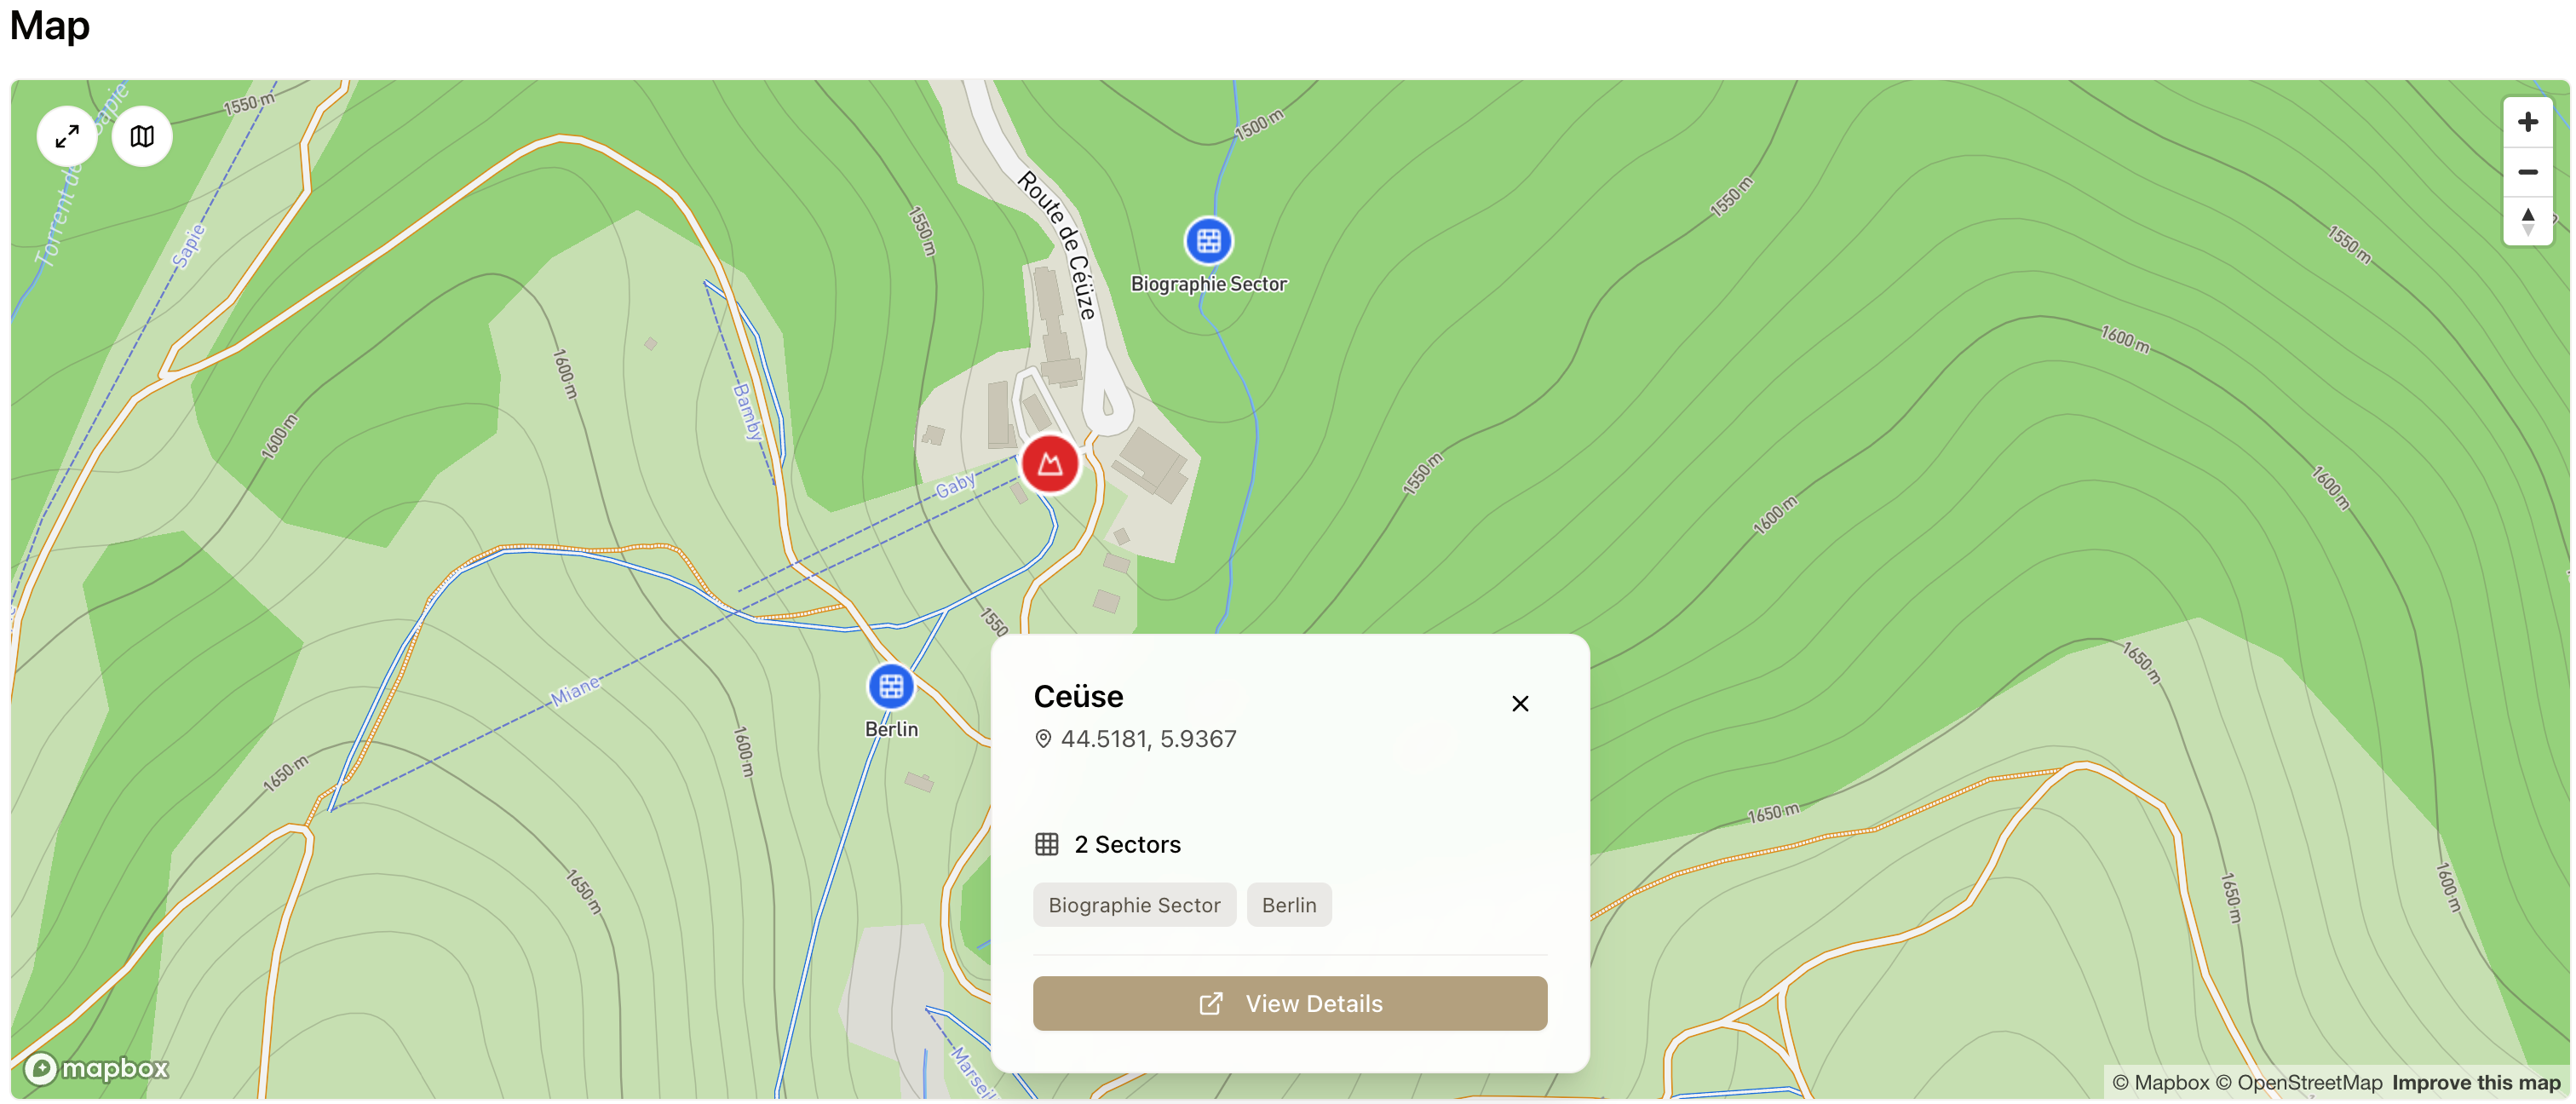
\includegraphics[width=0.9\textwidth]{images/implementacija/web/map_selected.png}
        \caption{Web aplikacija}
        \label{fig:geografska_karta_ceuse_web}
    \end{subfigure}
    \caption{Detaljan prikaz penjačke lokacije Ceuse}
    \label{fig:geografska_karta_ceuse_sidebyside}
\end{figure}

Odabirom oznake za pojedino penjalište, karta se automatski centrira i približava na tu lokaciju, prikazujući satelitski snimak područja. Na ovom detaljnom prikazu prikazana je oznaka za penjačku lokaciju, a i oznake za sve sektore. Ovakav prikaz je koristan za razumijevanje rasporeda sektora i planiranje kretanja na terenu. Na dnu prikaza nalazi se informativna kartica s osnovnim podacima o odabranoj lokaciji poput naziva, GPS koordinata i popisa dostupnih sektora. Korisniku se tada nude opcije za pregled detaljnih informacija o toj penjačkoj lokaciji ili sektorima. 

% \section{Pretraživanje penjačkih lokacija, sektora, penjačkih lokacija i korisnika}

Kako bi korisnici mogli brzo pronaći informacije, aplikacija omogućuje pretraživanje penjačkih lokacija, sektora, penjačkih smjerova i korisnika. Pristupom zaslonu za pretraživanje ili na web aplikaciji klikom na traku za pretraživanje u navigacijskoj traci, korisniku se prikazuje traka za unos teksta te, inicijalno, popis nedavno pregledanih stavki, što omogućuje brz povratak na prethodno pregledane elemente (slika~\ref{fig:pretrazivanje_sidebyside}).

\begin{figure}[H]
    \centering
    \begin{subfigure}[b]{0.35\textwidth}
        \centering
        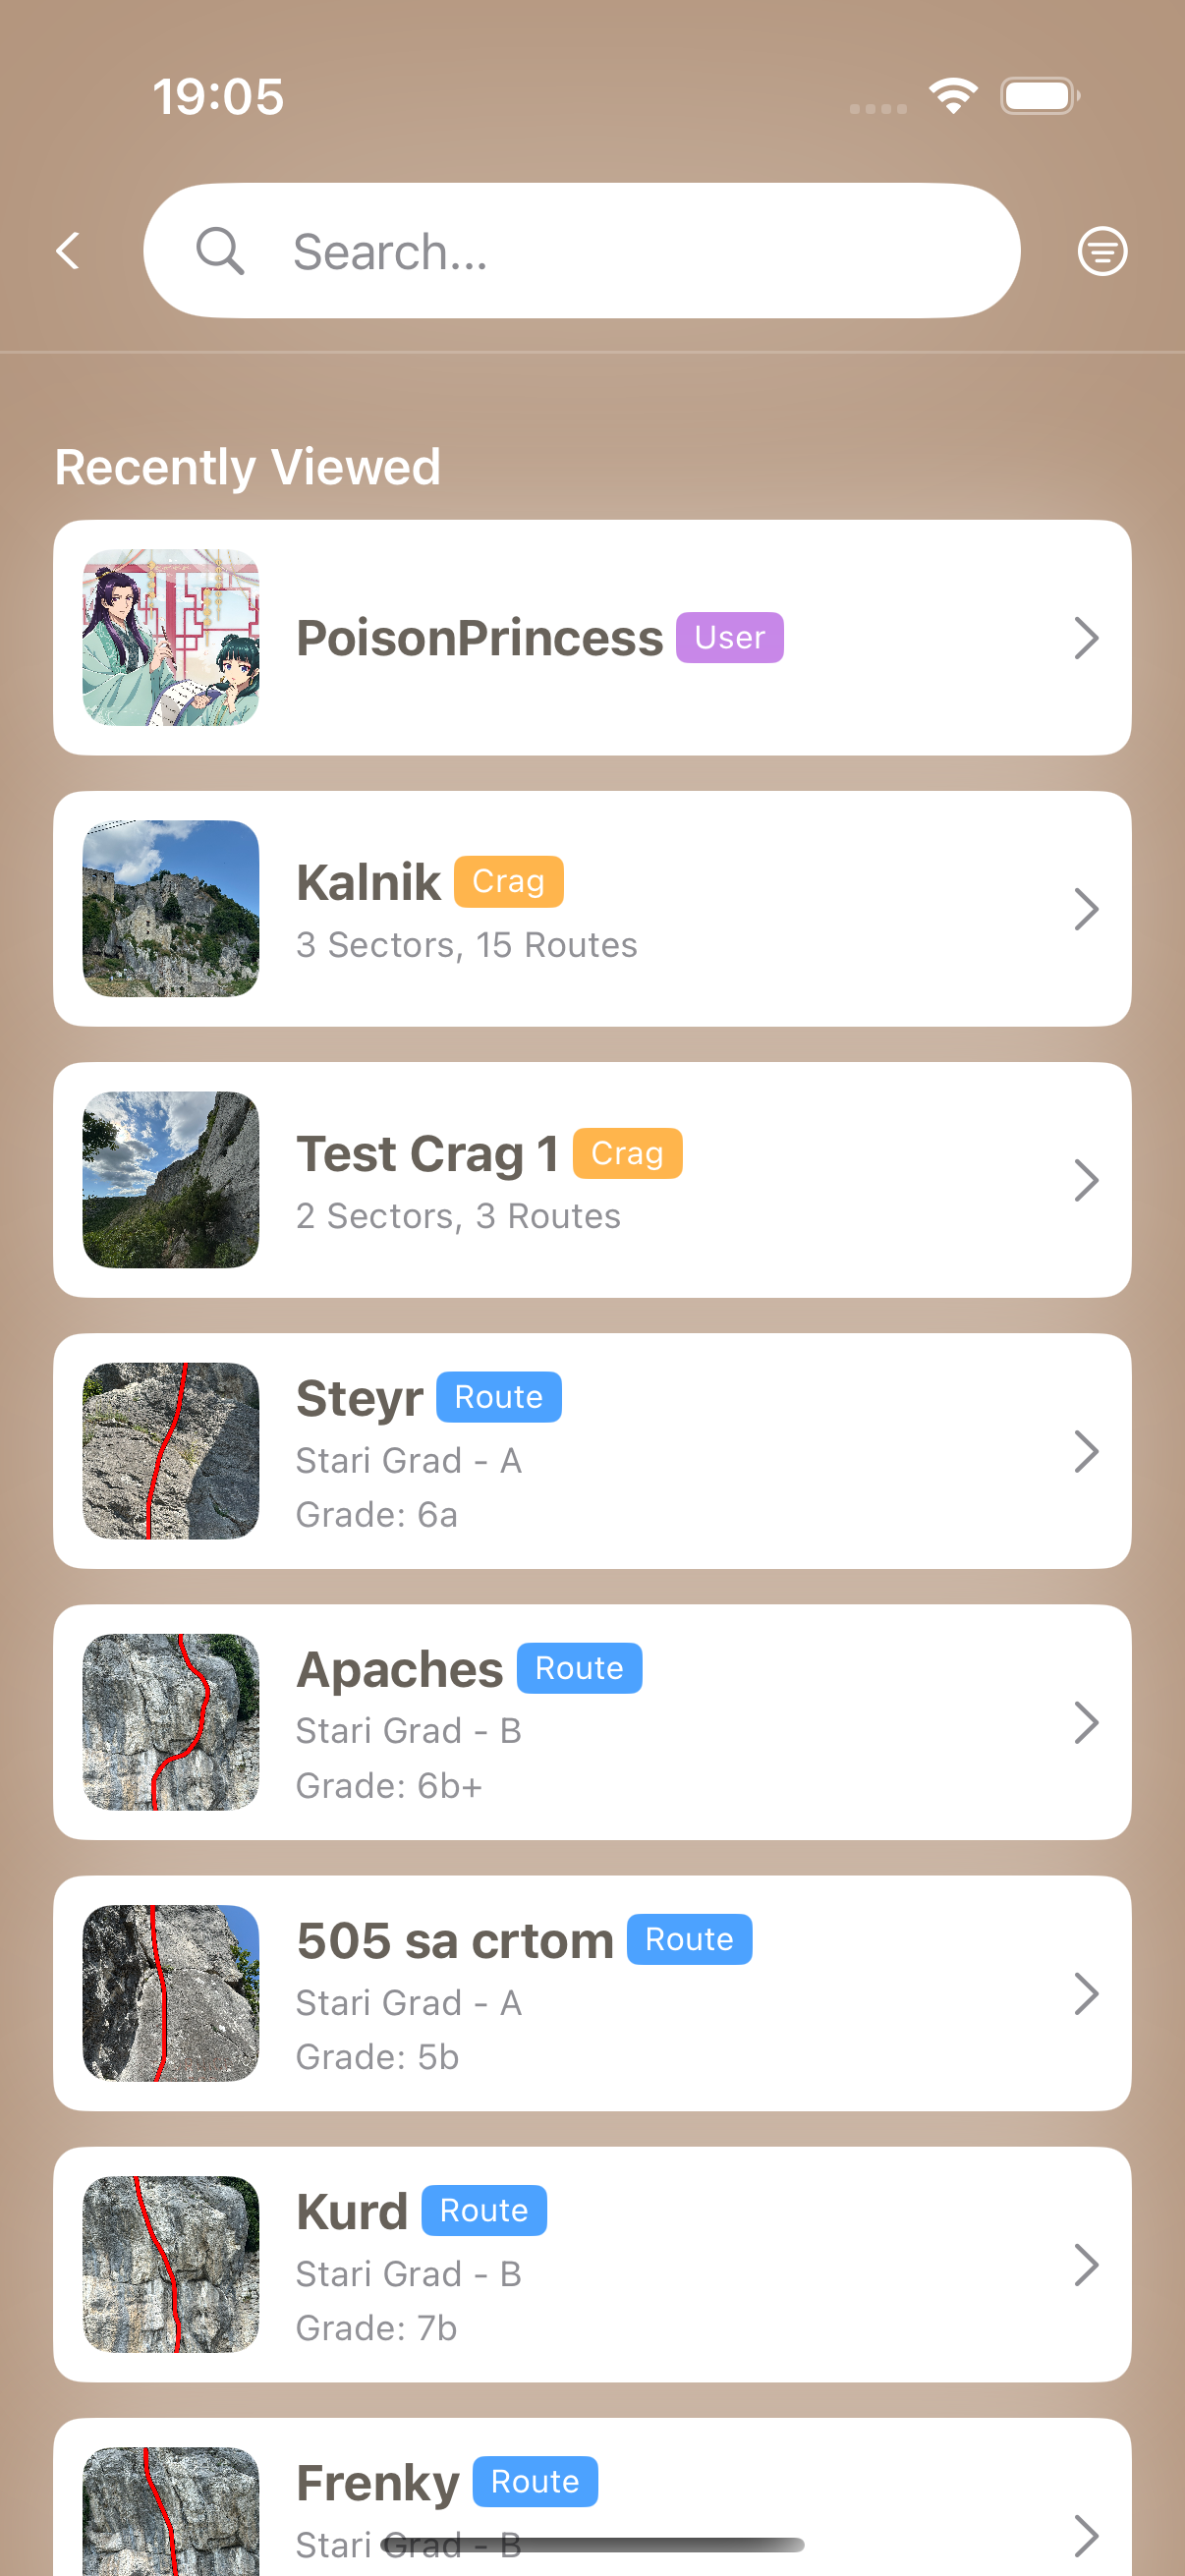
\includegraphics[width=\textwidth]{images/implementacija/search_default.png}
        \caption{Mobilna aplikacija}
        \label{fig:pretrazivanje_default}
    \end{subfigure}
    \hfill
    \begin{subfigure}[b]{0.6\textwidth}
        \centering
        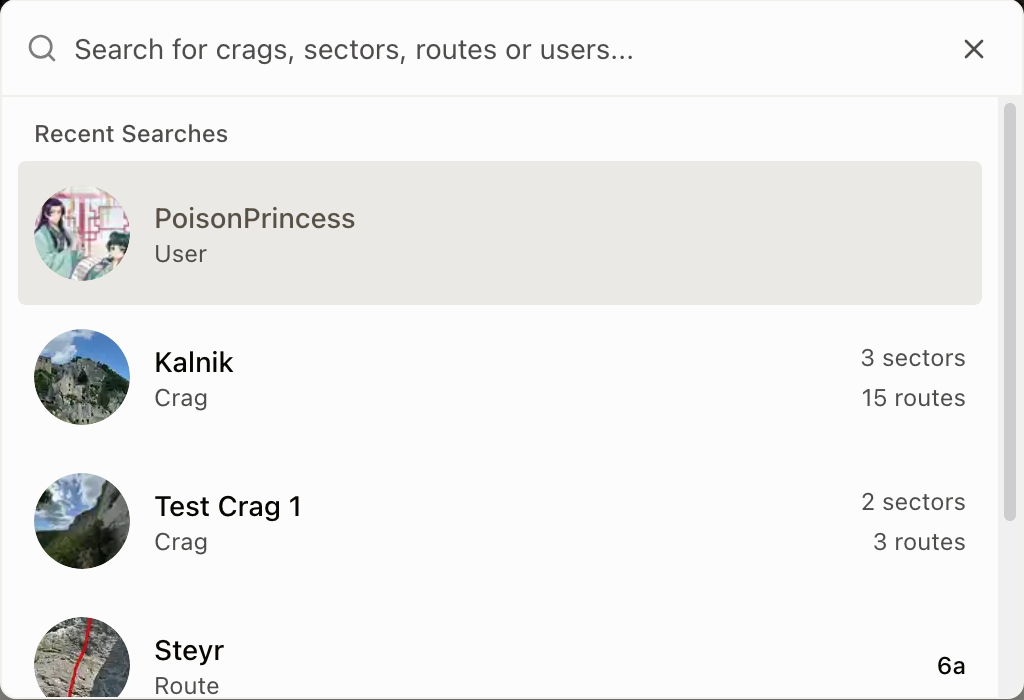
\includegraphics[width=\textwidth]{images/implementacija/web/search_default.png}
        \caption{Web aplikacija}
        \label{fig:pretrazivanje_searching}
    \end{subfigure}
    \caption{Inicijalno stanje pretraživanja - prikaz nedavno pregledanih stavki}
    \label{fig:pretrazivanje_sidebyside}
\end{figure}

Sustav pretraživanja je dinamičan i reagira na korisnikov unos. Upisivanjem pojma u traku za pretraživanje, aplikacija filtrira popis dostupnih penjačkih lokacija, sektora, penjačkih smjerova i korisnika te prikazuje relevantne rezultate iz više kategorija istovremeno (slika~\ref{fig:pretrazivanje_side_by_side}). 

\begin{figure}[H]
    \centering
    \begin{subfigure}[b]{0.35\textwidth}
        \centering
        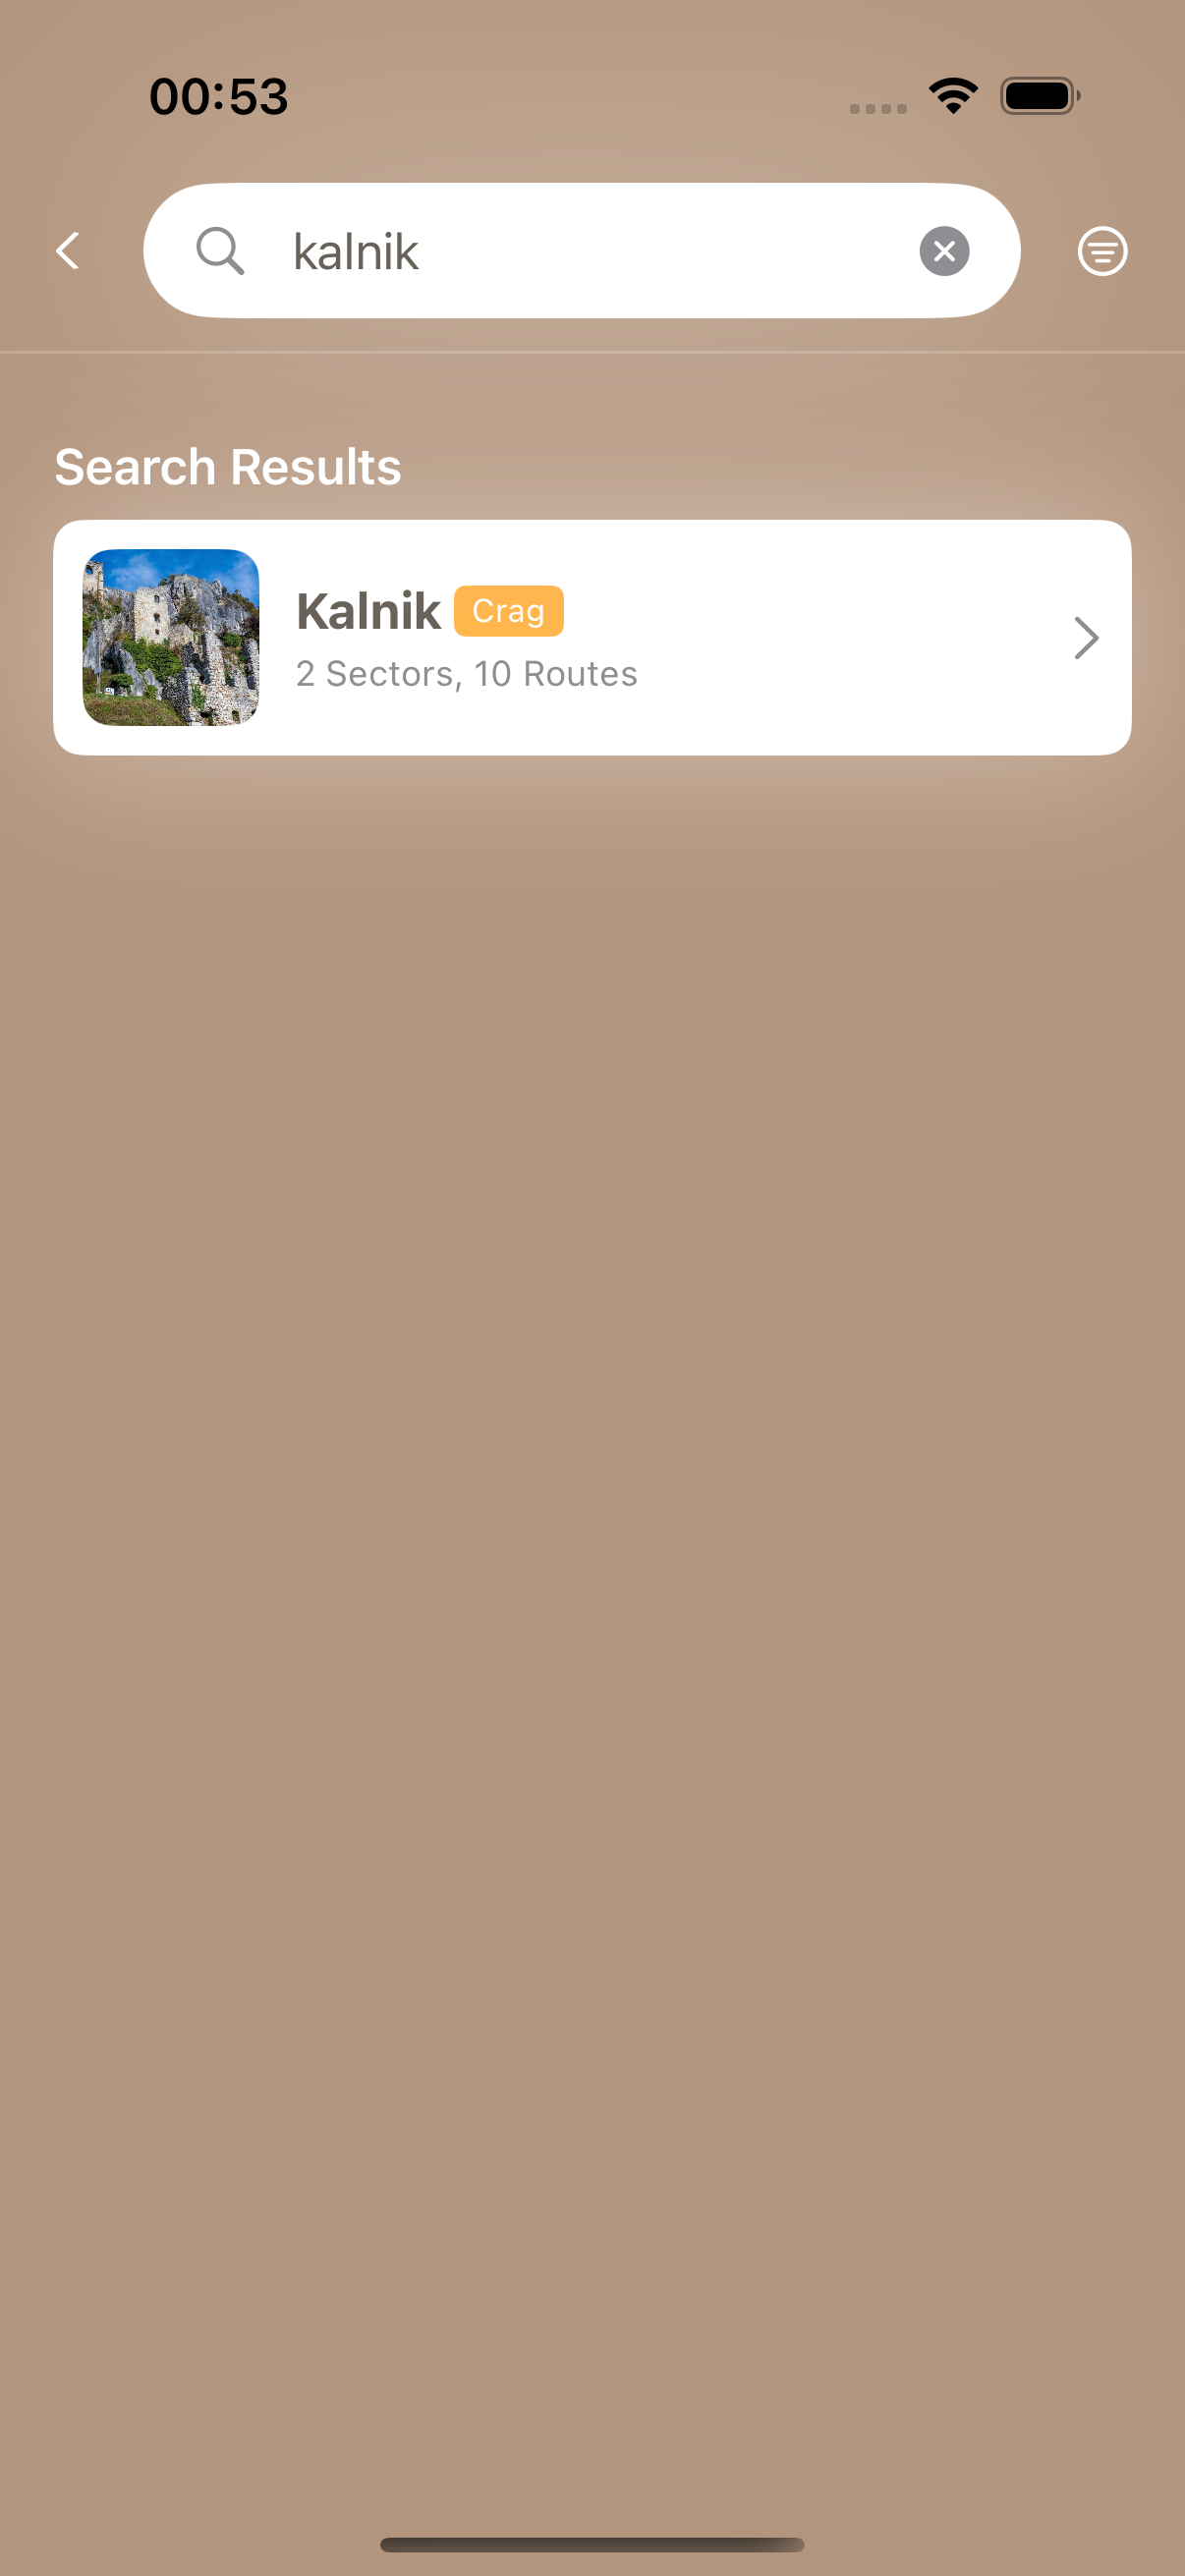
\includegraphics[width=\textwidth]{images/implementacija/search_searching.png}
        \caption{Mobilna aplikacija}
        \label{fig:pretrazivanje_web_1}
    \end{subfigure}
    \hfill
    \begin{subfigure}[b]{0.6\textwidth}
        \centering
        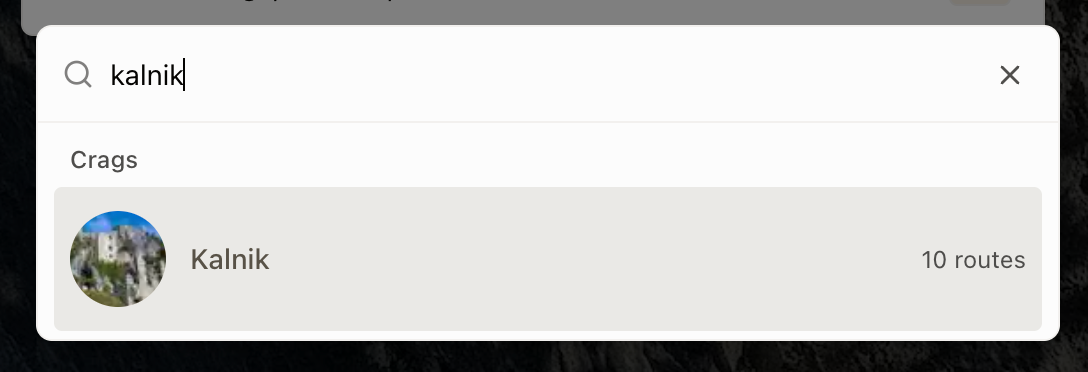
\includegraphics[width=\textwidth]{images/implementacija/web/search_searching.png}
        \caption{Web aplikacija}
        \label{fig:pretrazivanje_web_2}
    \end{subfigure}
    \caption{Funkcionalnost pretraživanja}
    \label{fig:pretrazivanje_side_by_side}
\end{figure}

Svaki rezultat pretrage prikazan je u obliku pregleda kartica koje sadrže informacije poput naziva i tipa sadržaja, te dodatne podatke ovisno o tipu sadržaja. Penjačke lokacije sadrže broj sektora i penjačkih smjerova, sektori broj penjačkih smjerova, a korisnici broj penjačkih smjerova koje su popeli. Odabirom bilo kojeg rezultata, korisnik se preusmjerava na odgovarajući detaljni prikaz. 


% \section{Detalji penjališta}

\begin{figure}[H]
    \centering
    \begin{subfigure}[b]{\textwidth}
        \centering
        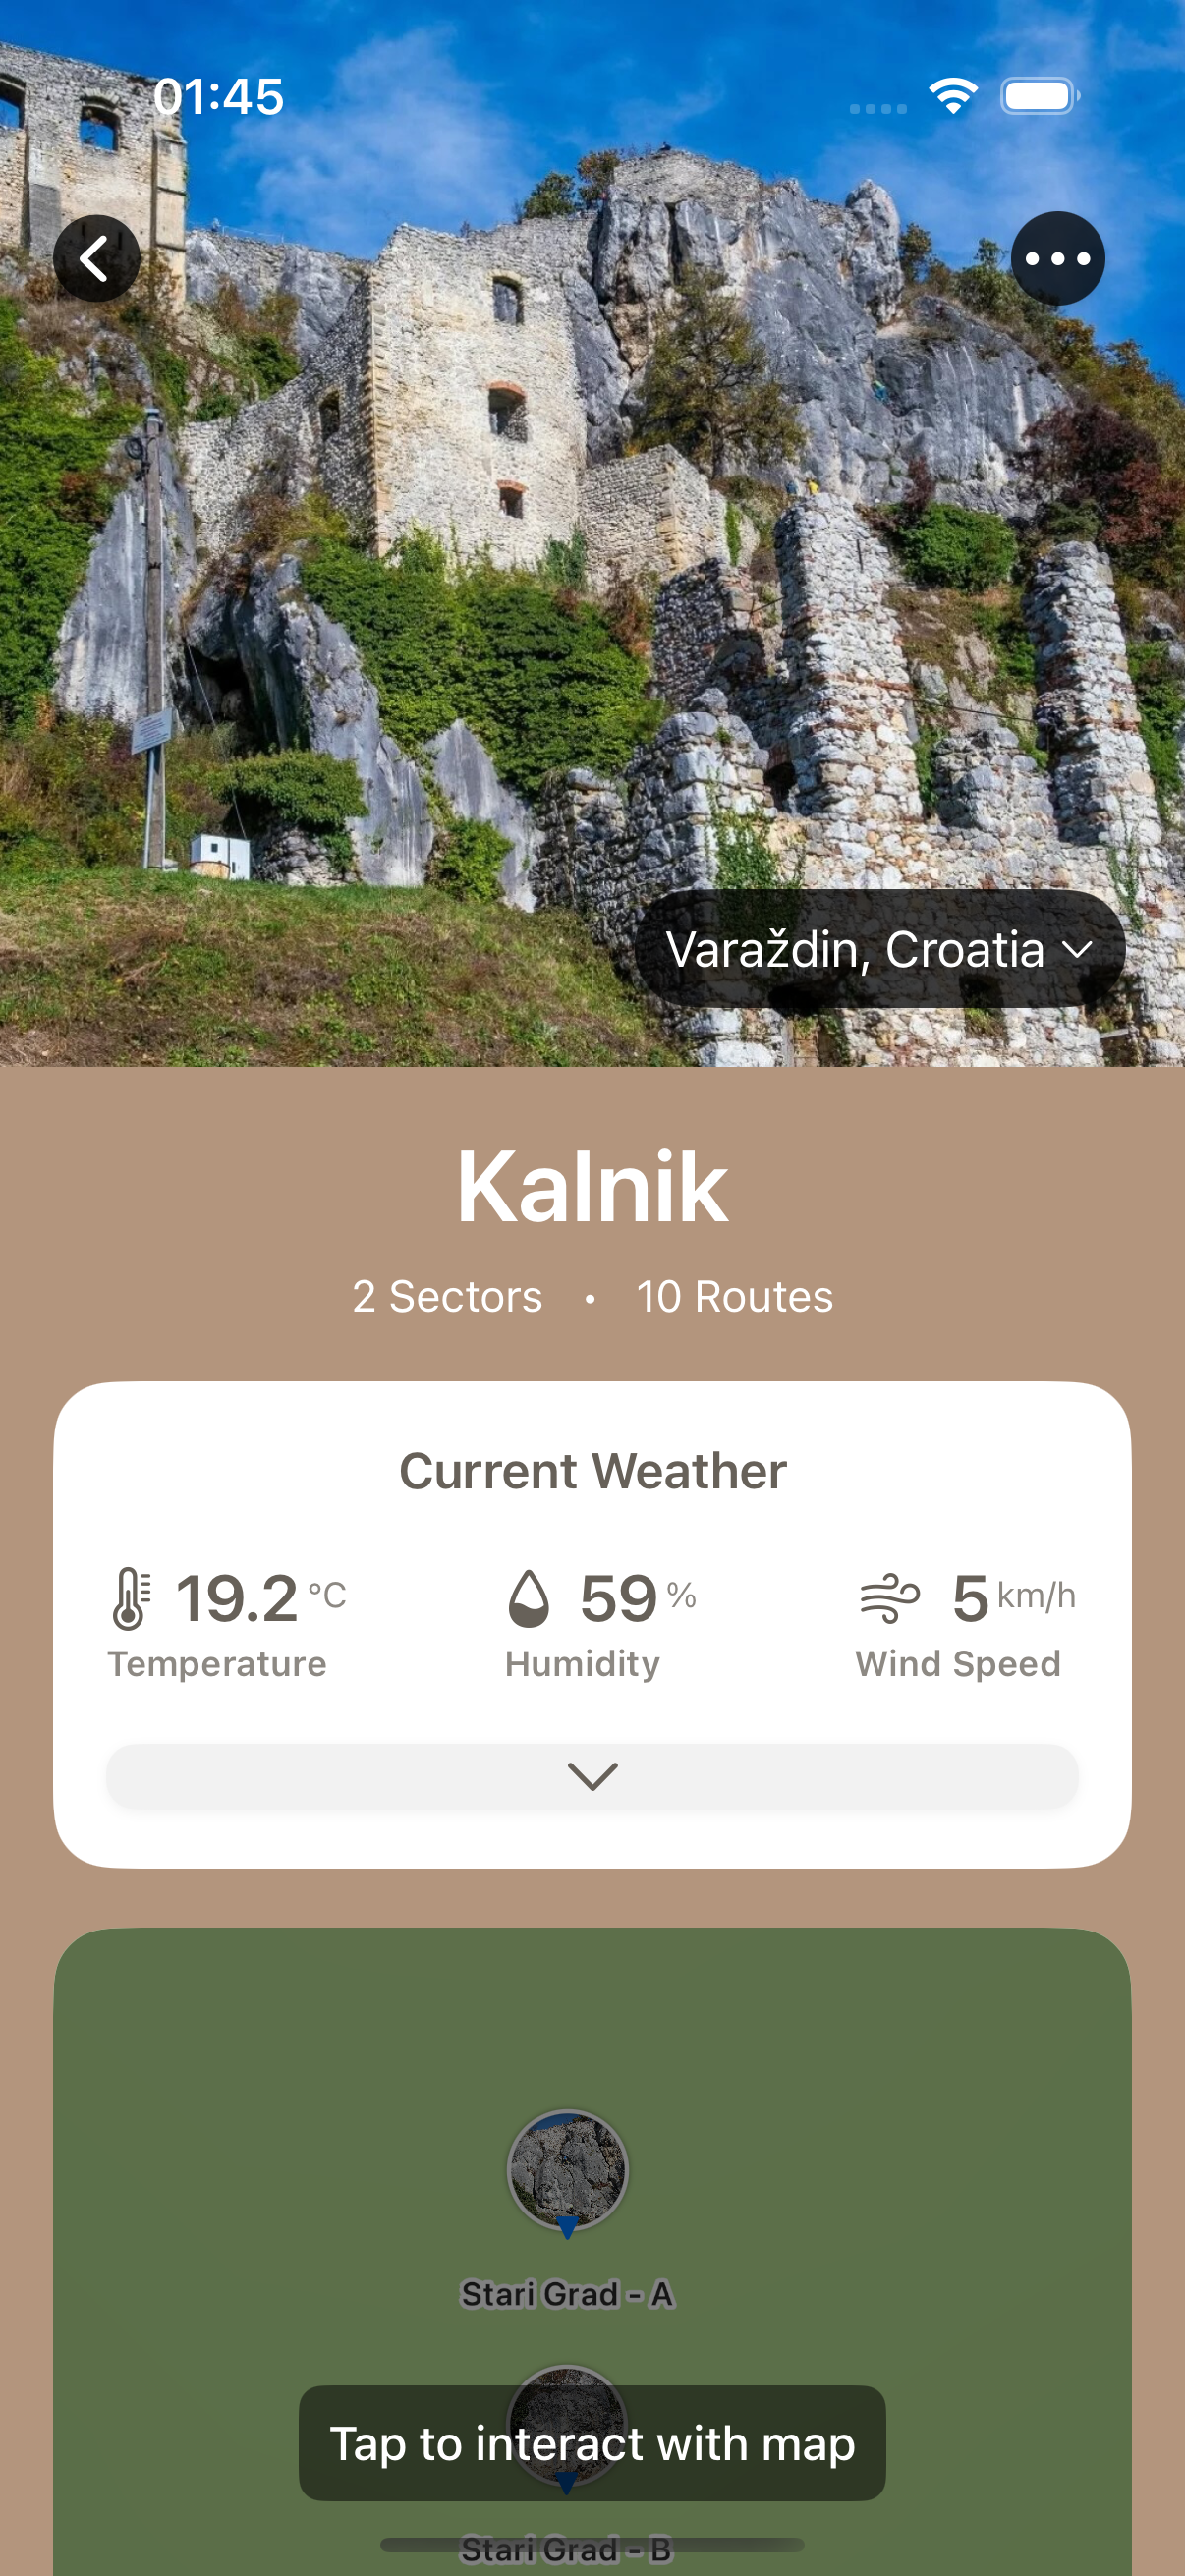
\includegraphics[width=0.3\textwidth]{images/implementacija/crag-details/crag-details-top.png}
        \caption{Mobilna aplikacija}
        \label{fig:detalji_penjališta_mob}
    \end{subfigure}
    \hfill
    \begin{subfigure}[b]{\textwidth}
        \centering
        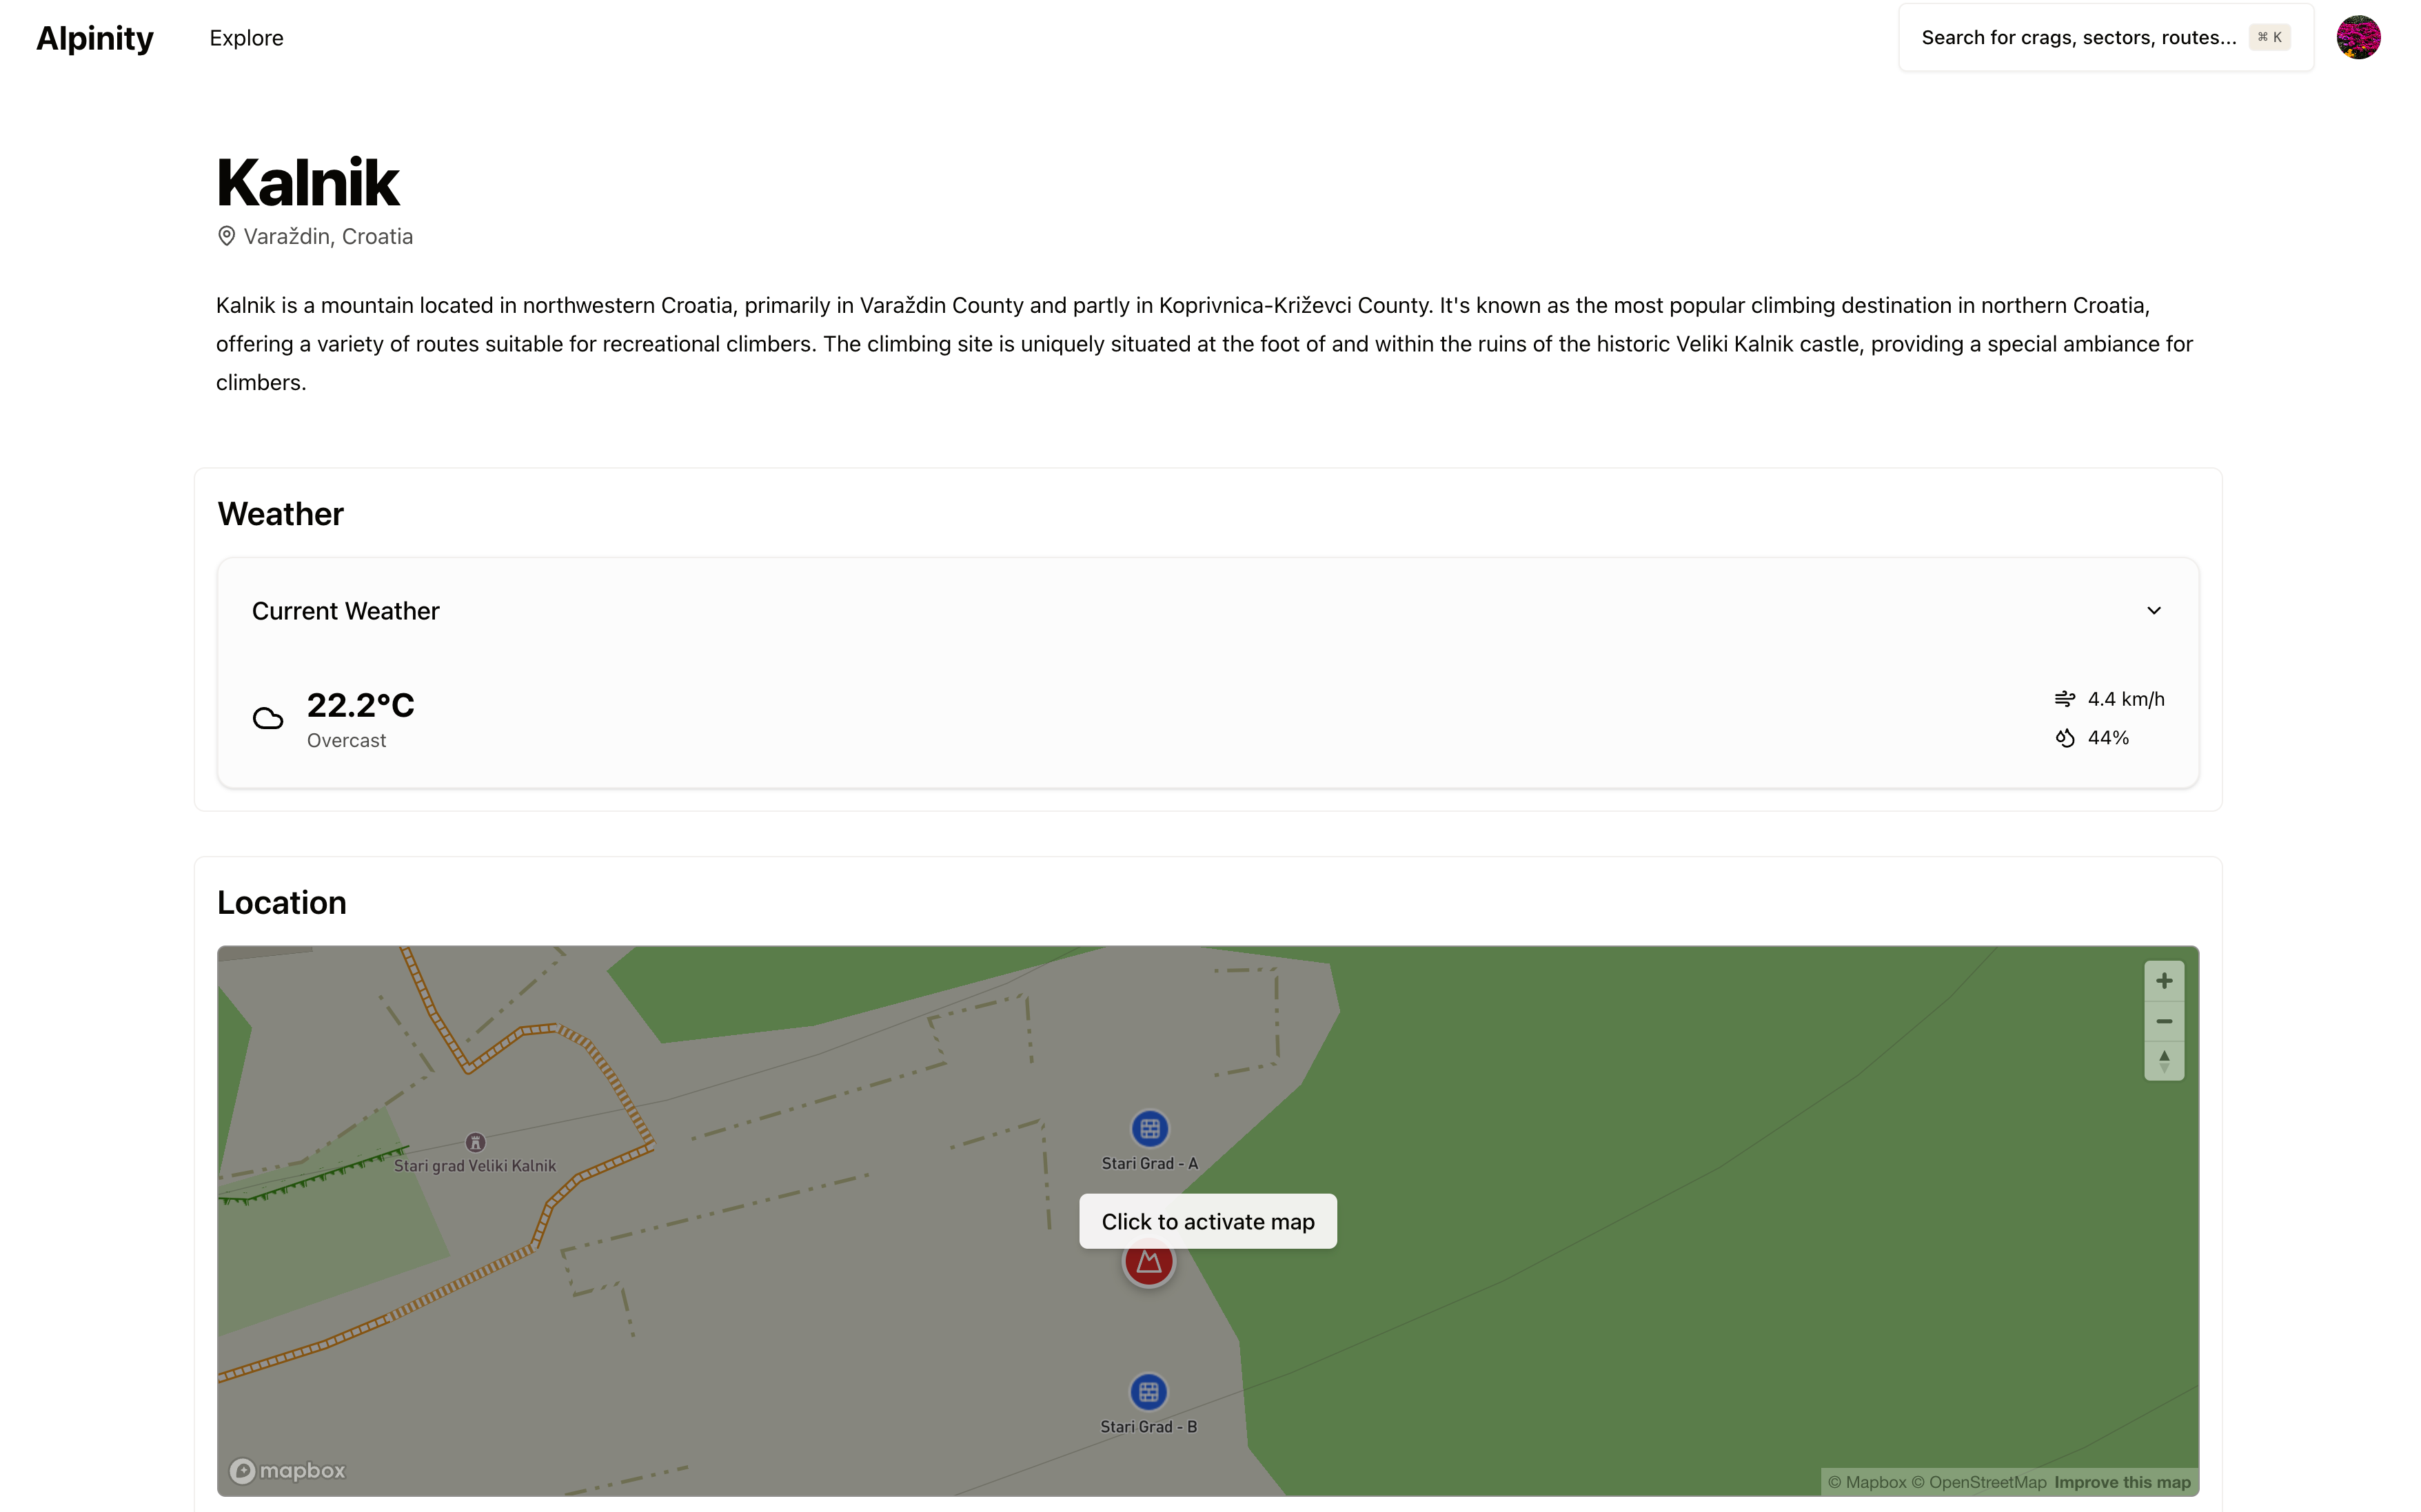
\includegraphics[width=0.9\textwidth]{images/implementacija/web/crag-details/crag-details-top.png}
        \caption{Web aplikacija}
        \label{fig:detalji_penjališta_web}
    \end{subfigure}
    \caption{Detalji penjališta na mobilnoj i web aplikaciji}
    \label{fig:detalji_penjališta_1}
\end{figure}

Odabirom penjališta iz pretrage, s geografske karte ili drugih pregleda, korisnik pristupa zaslonu s detaljnim informacijama o penjalištu (slika~\ref{fig:detalji_penjališta_1}). Zaslon je podijeljen na nekoliko cjelina. Na vrhu se nalazi istaknuta fotografija penjališta, zajedno s nazivom i osnovnim podacima o broju sektora i penjačkih smjerova. 
Na web aplikaciji nalazi se isti prikaz, ali s manjim promjenama. Slika penjališta nalazi se ispod geografske karte, a broj sektora i penjačkih smjerova nalazi se u prikazu sektora i penjačkih smjerova.

\begin{figure}[H]
    \centering
    \begin{subfigure}[b]{\textwidth}
        \centering
        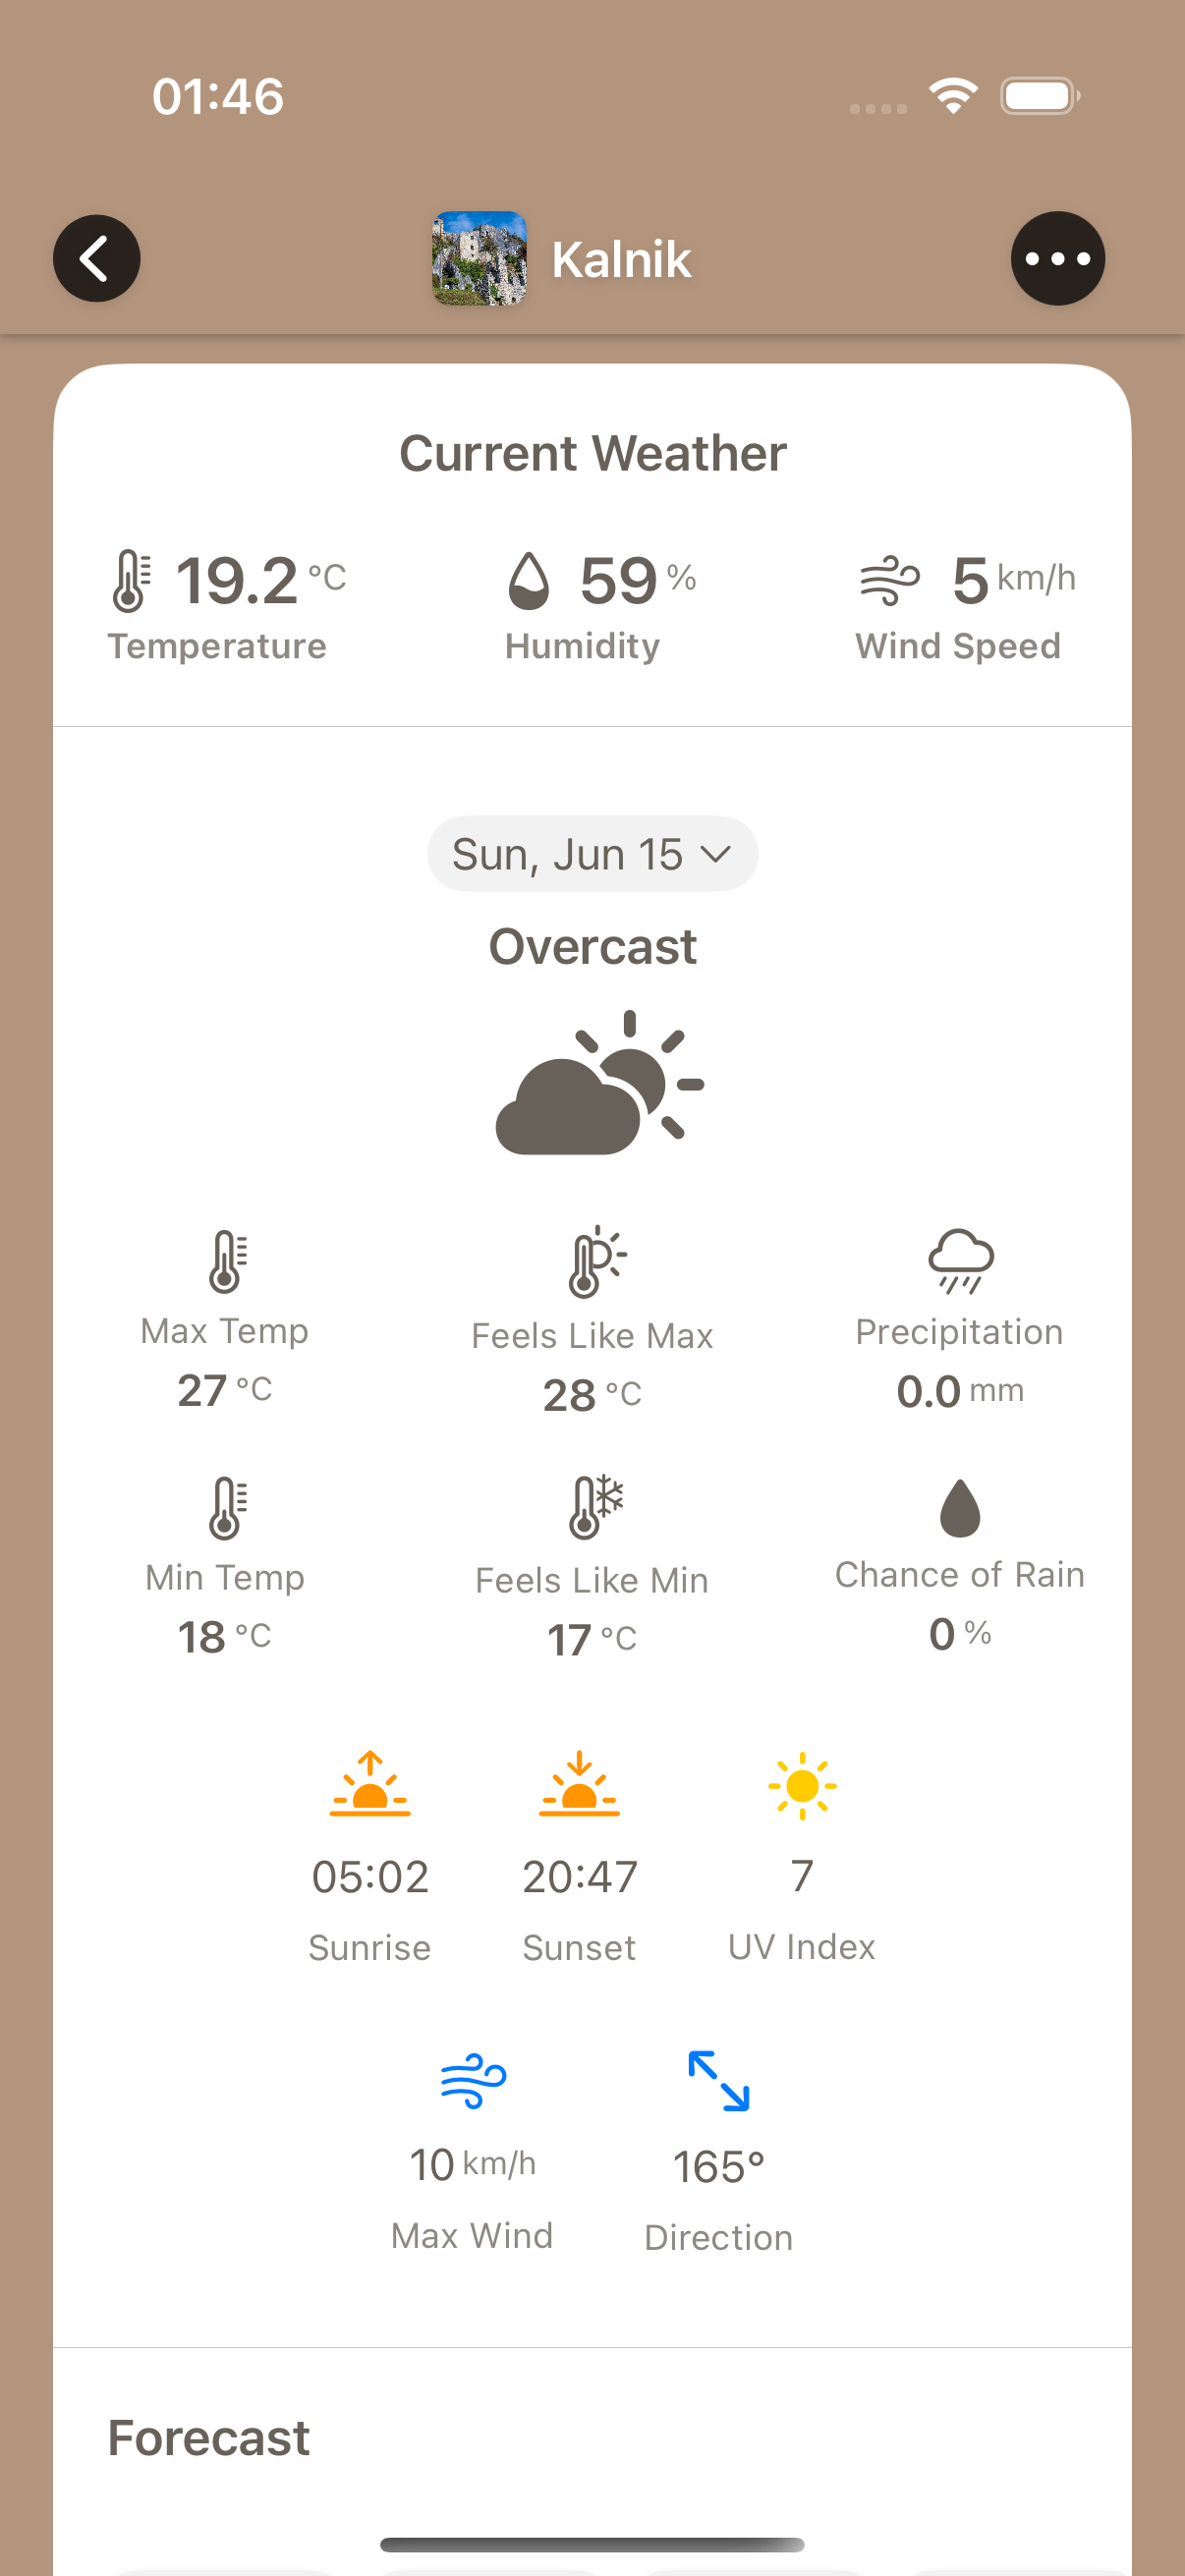
\includegraphics[width=0.35\textwidth]{images/implementacija/crag-details/crag-weather-1.png}
        \caption{Mobilna aplikacija}
        \label{fig:vremenska_prognoza_mob}
    \end{subfigure}
    \hfill
    \begin{subfigure}[b]{\textwidth}
        \centering
        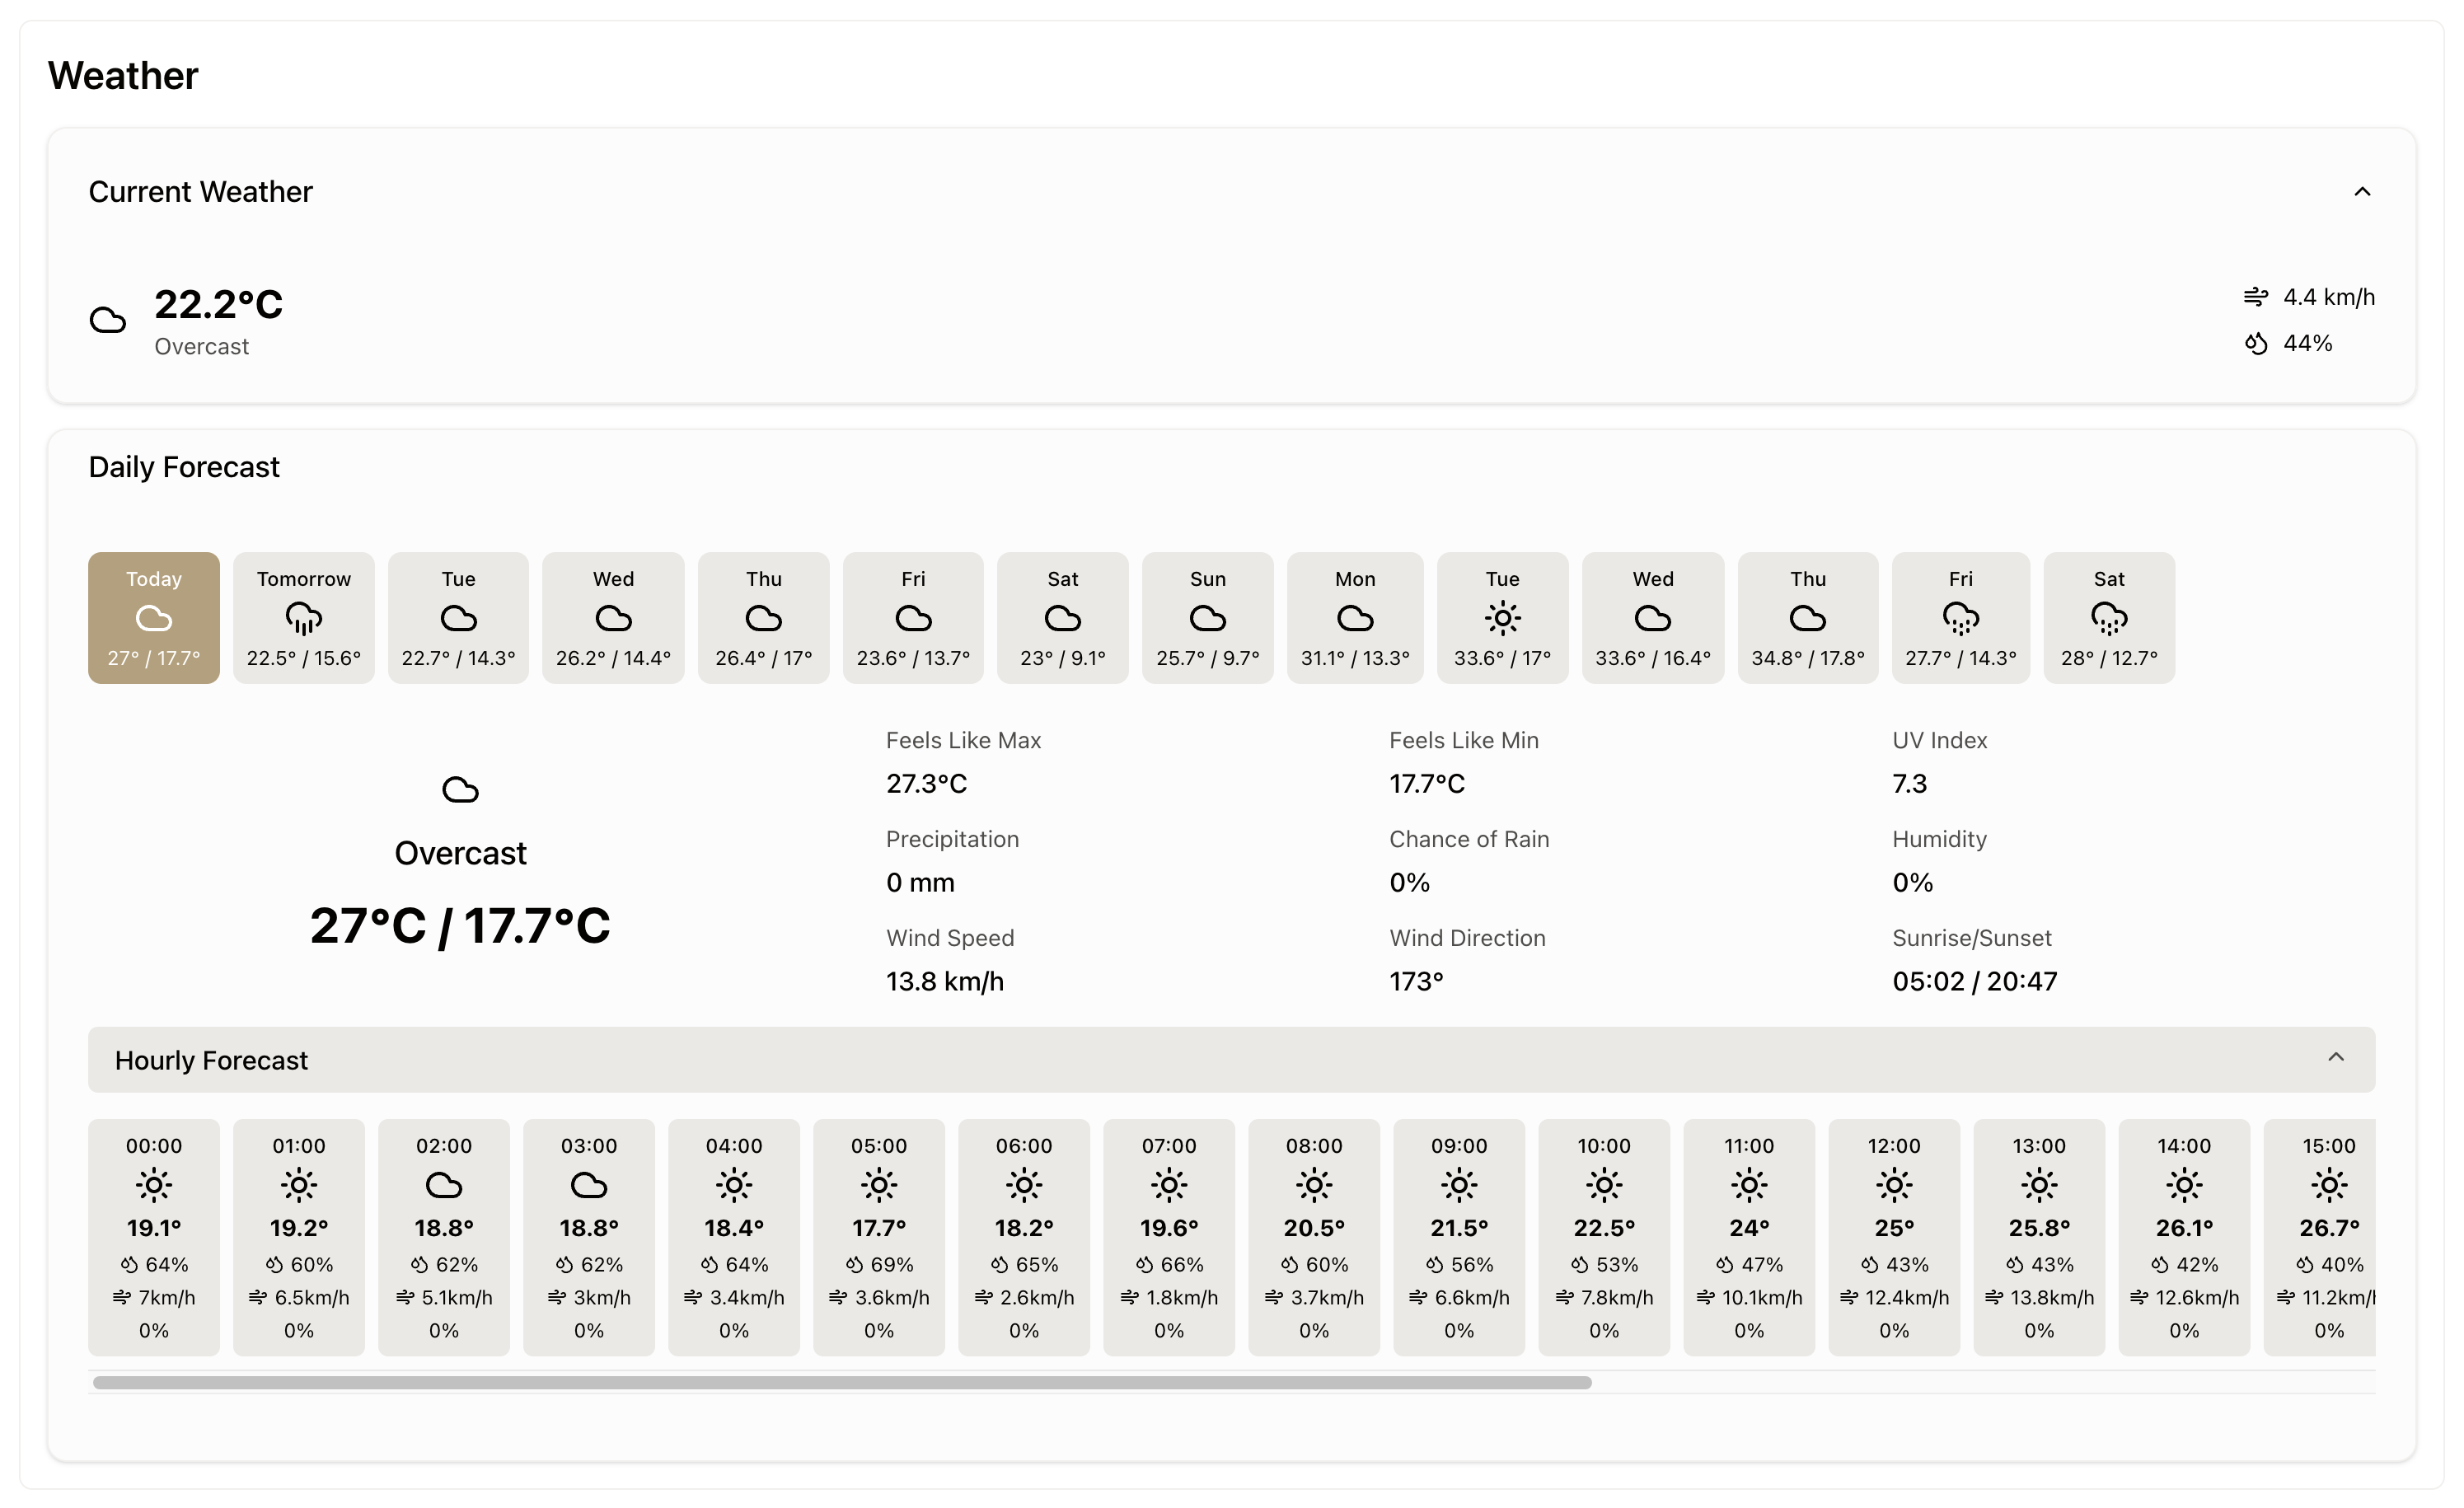
\includegraphics[width=0.9\textwidth]{images/implementacija/web/crag-details/crag-weather.png}
        \caption{Web aplikacija}
        \label{fig:vremenska_prognoza_web}
    \end{subfigure}
    \caption{Vremenska prognoza na mobilnoj i web aplikaciji}
    \label{fig:vremenska_prognoza}
\end{figure}

Odmah ispod, nalazi se komponenta s vremenskom prognozom (slika~\ref{fig:vremenska_prognoza}). Ona prikazuje trenutne vremenske uvjete, kao i detaljnu prognozu po satima za sljedećih 14 dana. Detaljna prognoza uključuje temperaturu, vjerojatnost i količina padalina, brzinu vjetra, UV indeks i ostale relevantne podatke. Ova funkcionalnost je važna za planiranje penjačkih izleta.


Nakon komponente vremenske prognoze sljedi interaktivna karta penjališta koja prikazuje precizne lokacije svih sektora, omogućujući korisniku lako snalaženje i planiranje kretanja između njih (slika~\ref{fig:interaktivna_karta}). 

\begin{figure}[H]
    \centering
    \begin{subfigure}[b]{\textwidth}
        \centering
        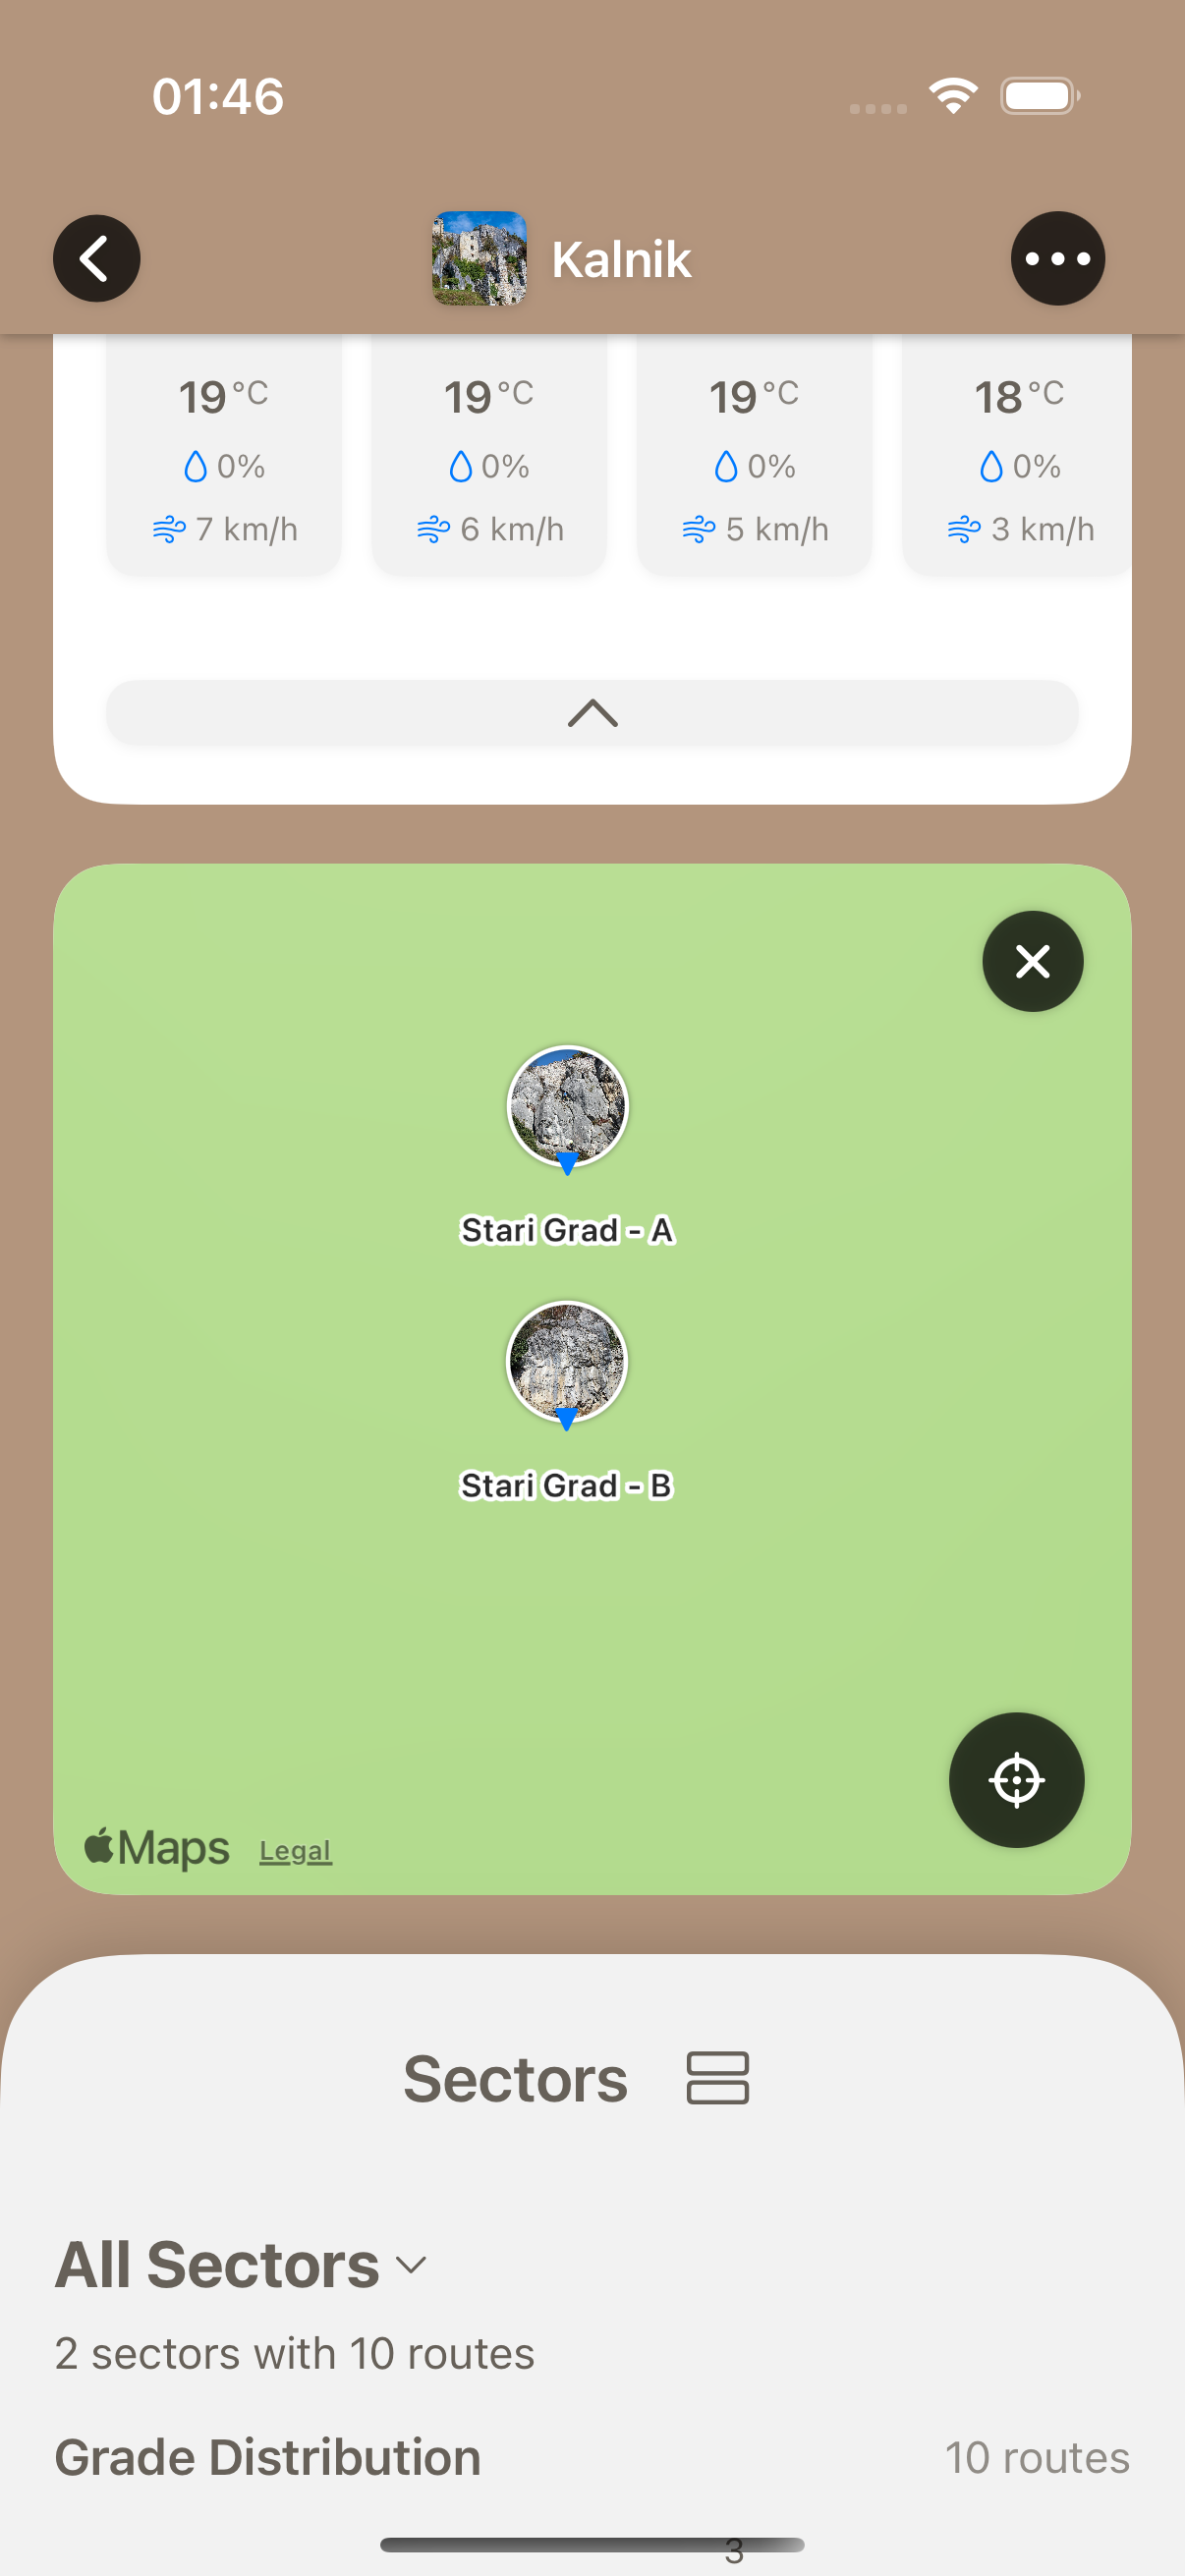
\includegraphics[width=0.35\textwidth]{images/implementacija/crag-details/crag-map.png}
        \caption{Mobilna aplikacija}
        \label{fig:interaktivna_karta_mob}
    \end{subfigure}
    \hfill
    \begin{subfigure}[b]{\textwidth}
        \centering
        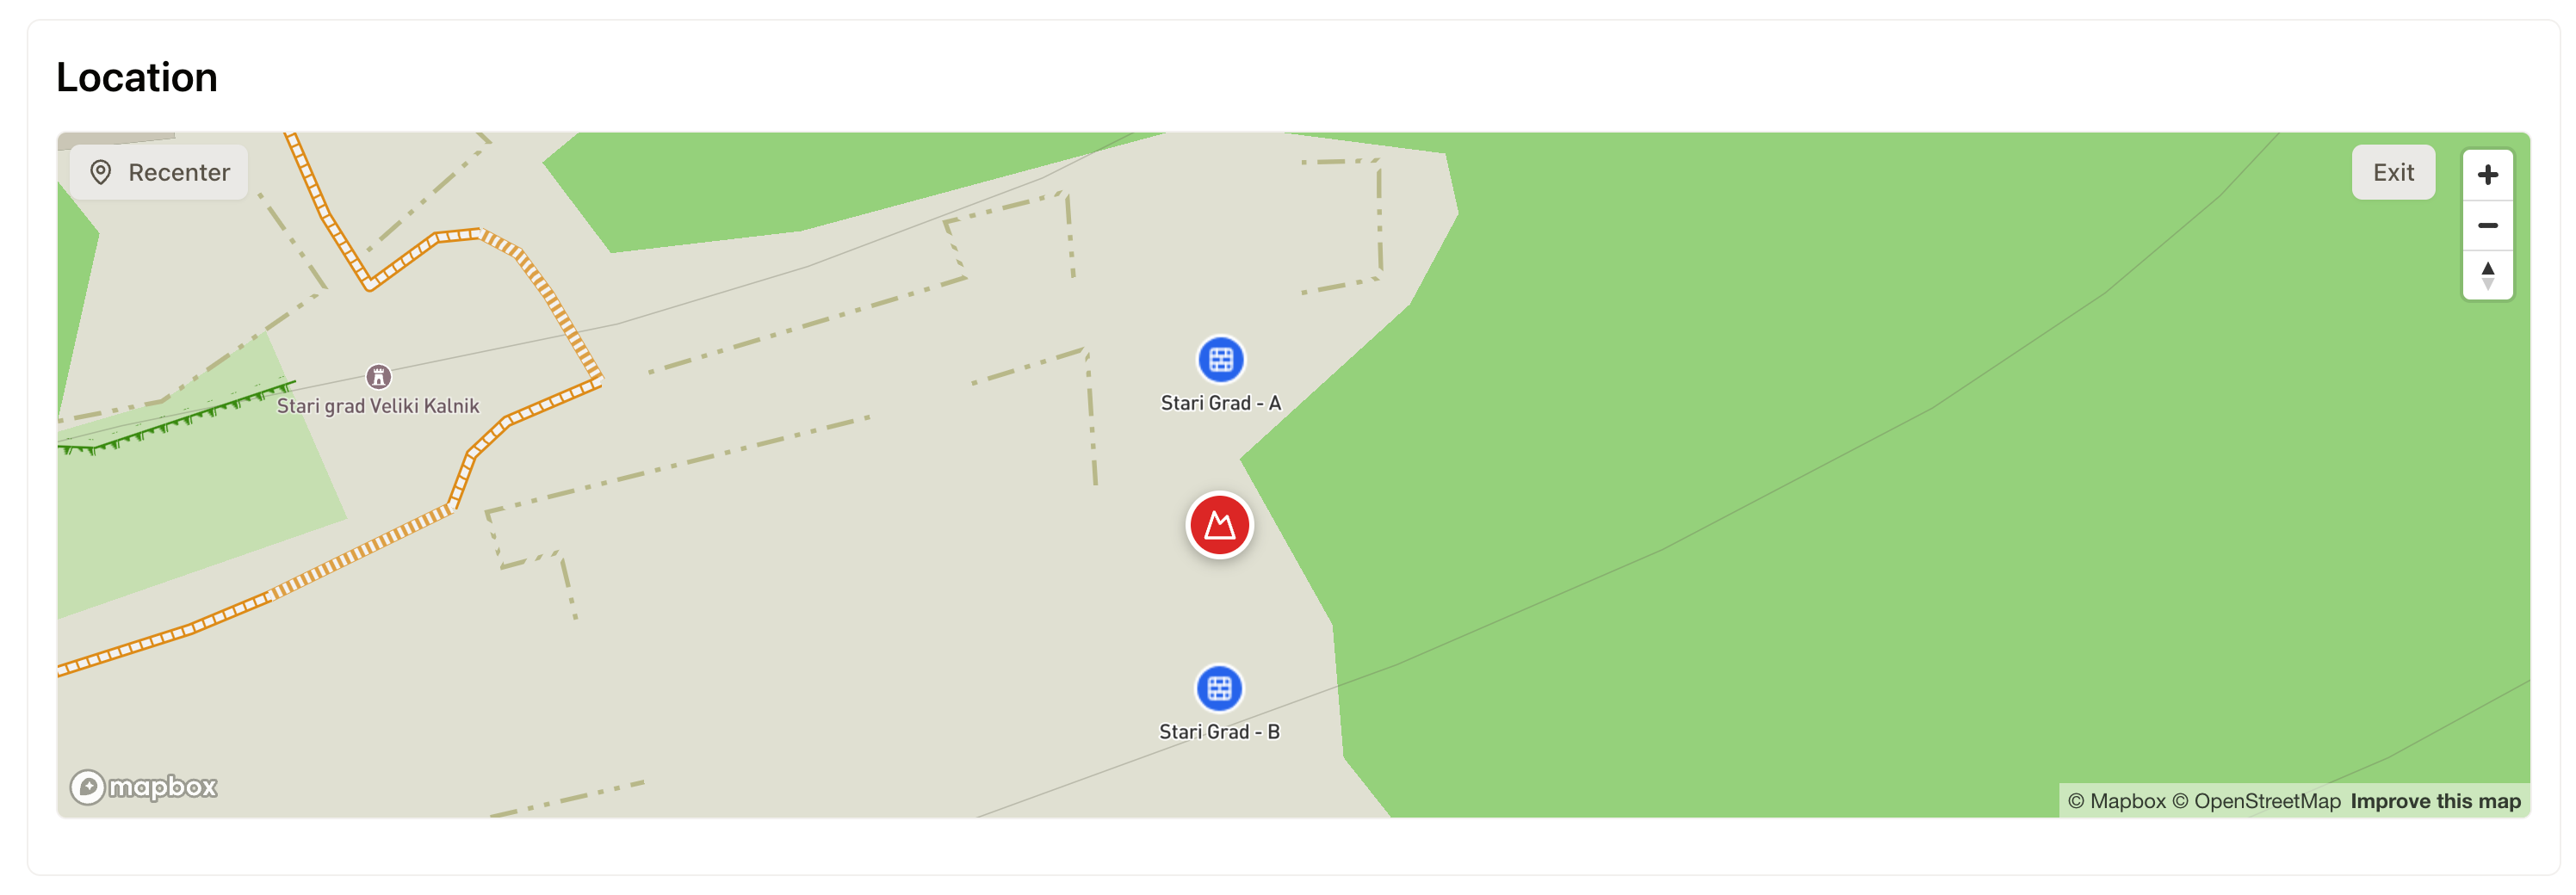
\includegraphics[width=0.9\textwidth]{images/implementacija/web/crag-details/crag-map.png}
        \caption{Web aplikacija}
        \label{fig:interaktivna_karta_web}
    \end{subfigure}
    \caption{Interaktivna karta penjališta}
    \label{fig:interaktivna_karta}
\end{figure}

Ispod karte nalazi se prikaz detalja za sektore. Prije ikakvih odabira, korisniku se prikazuje popis svih penjačkih smjerova grupiranih po sektorima te distribucija težina na penjalištu (slika~\ref{fig:prikaz_detalja_za_sektore}). 

\begin{figure}[H]
    \centering
    \begin{subfigure}[b]{0.4\textwidth}
        \centering
        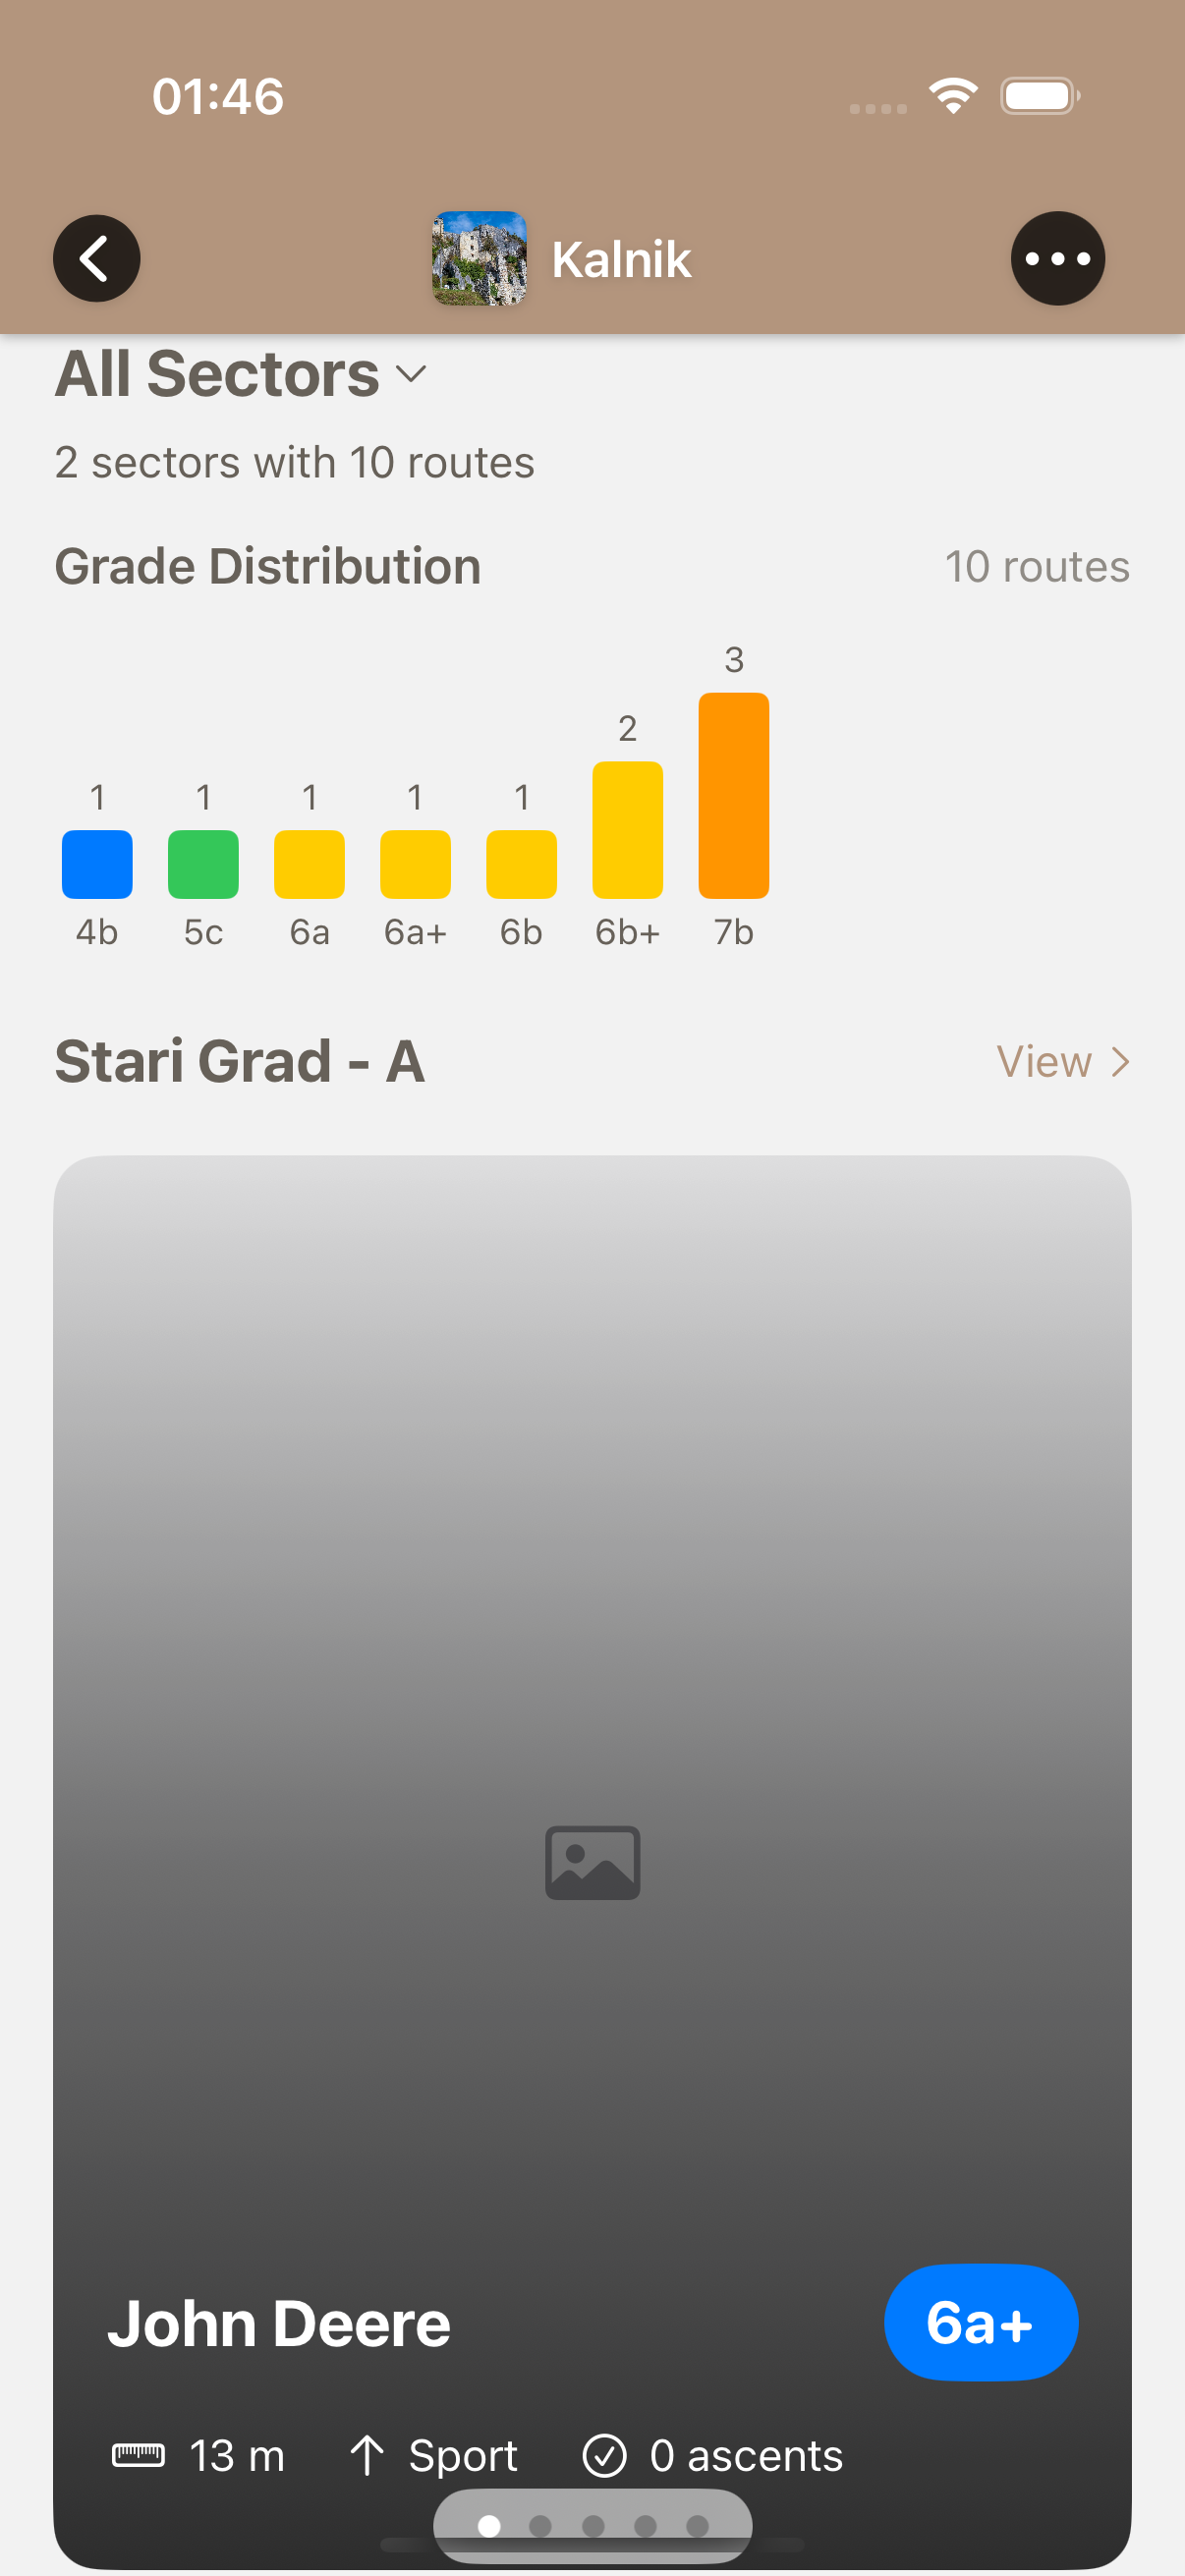
\includegraphics[width=0.7\textwidth]{images/implementacija/crag-details/crag-all-sectors-tabs.png}
        \caption{Mobilna aplikacija}
        \label{fig:prikaz_detalja_za_sektore_mob}
    \end{subfigure}
    \hfill
    \begin{subfigure}[b]{0.55\textwidth}
        \centering
        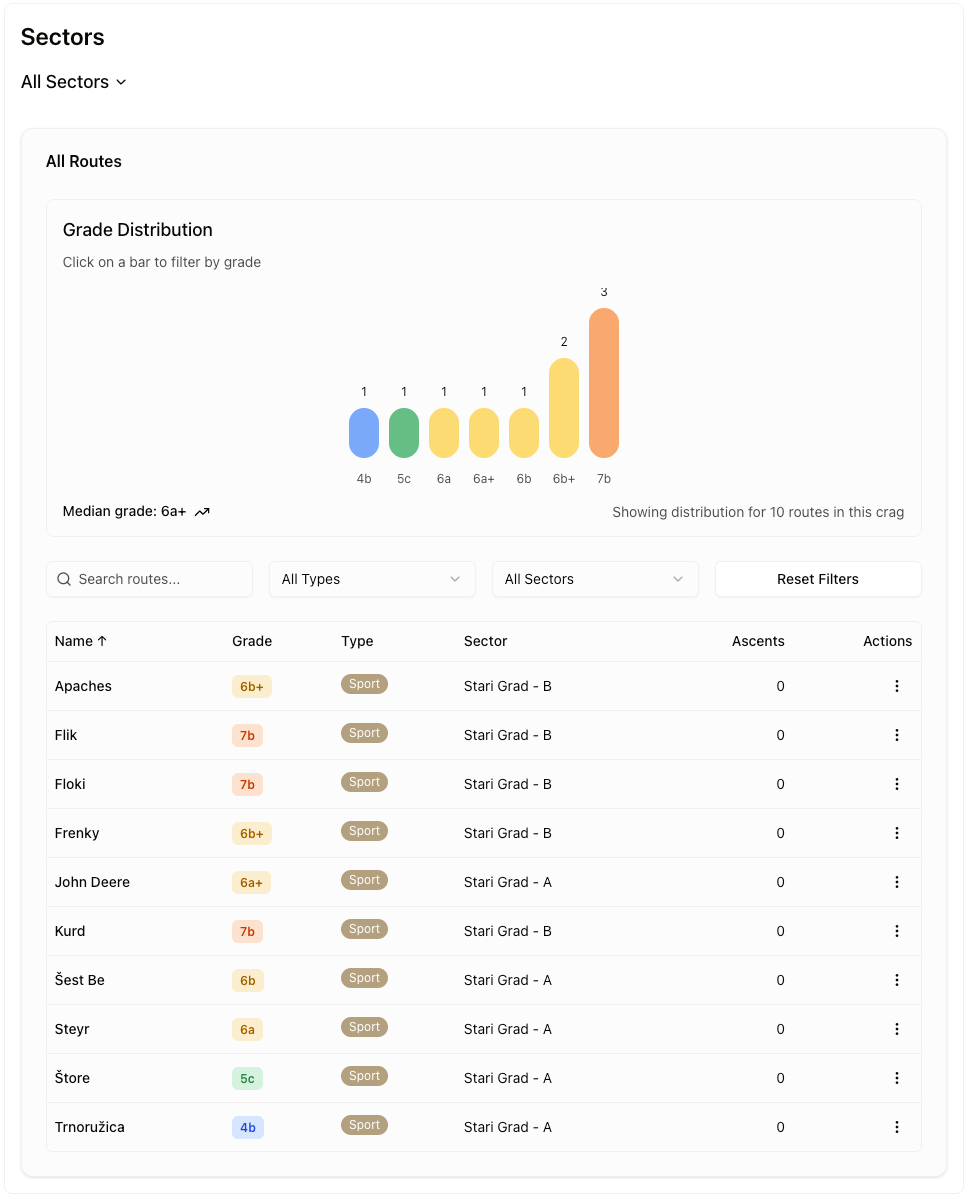
\includegraphics[width=1\textwidth]{images/implementacija/web/crag-details/crag-all-sectors.png}
        \caption{Web aplikacija}
        \label{fig:prikaz_detalja_za_sektore_web}
    \end{subfigure}
    \caption{Prikaz detalja za sektore}
    \label{fig:prikaz_detalja_za_sektore}
\end{figure}

Klikom na određenu težinu u grafu filtriraju se svi penjački smjerovi koji pripadaju odabranoj težini. Lista penjačkih smjerova na mobilnoj aplikaciji je horizontalna lista koja prikazuje penjački smjer u većem formatu kako bi se mogla bolje vidjeti slika penjačkog smjera. Preko slike nalaze se detalji o penjačkom smjeru poput naziva, težine, dužine, tipa i broja uspona.

\begin{figure}[H]
    \centering
    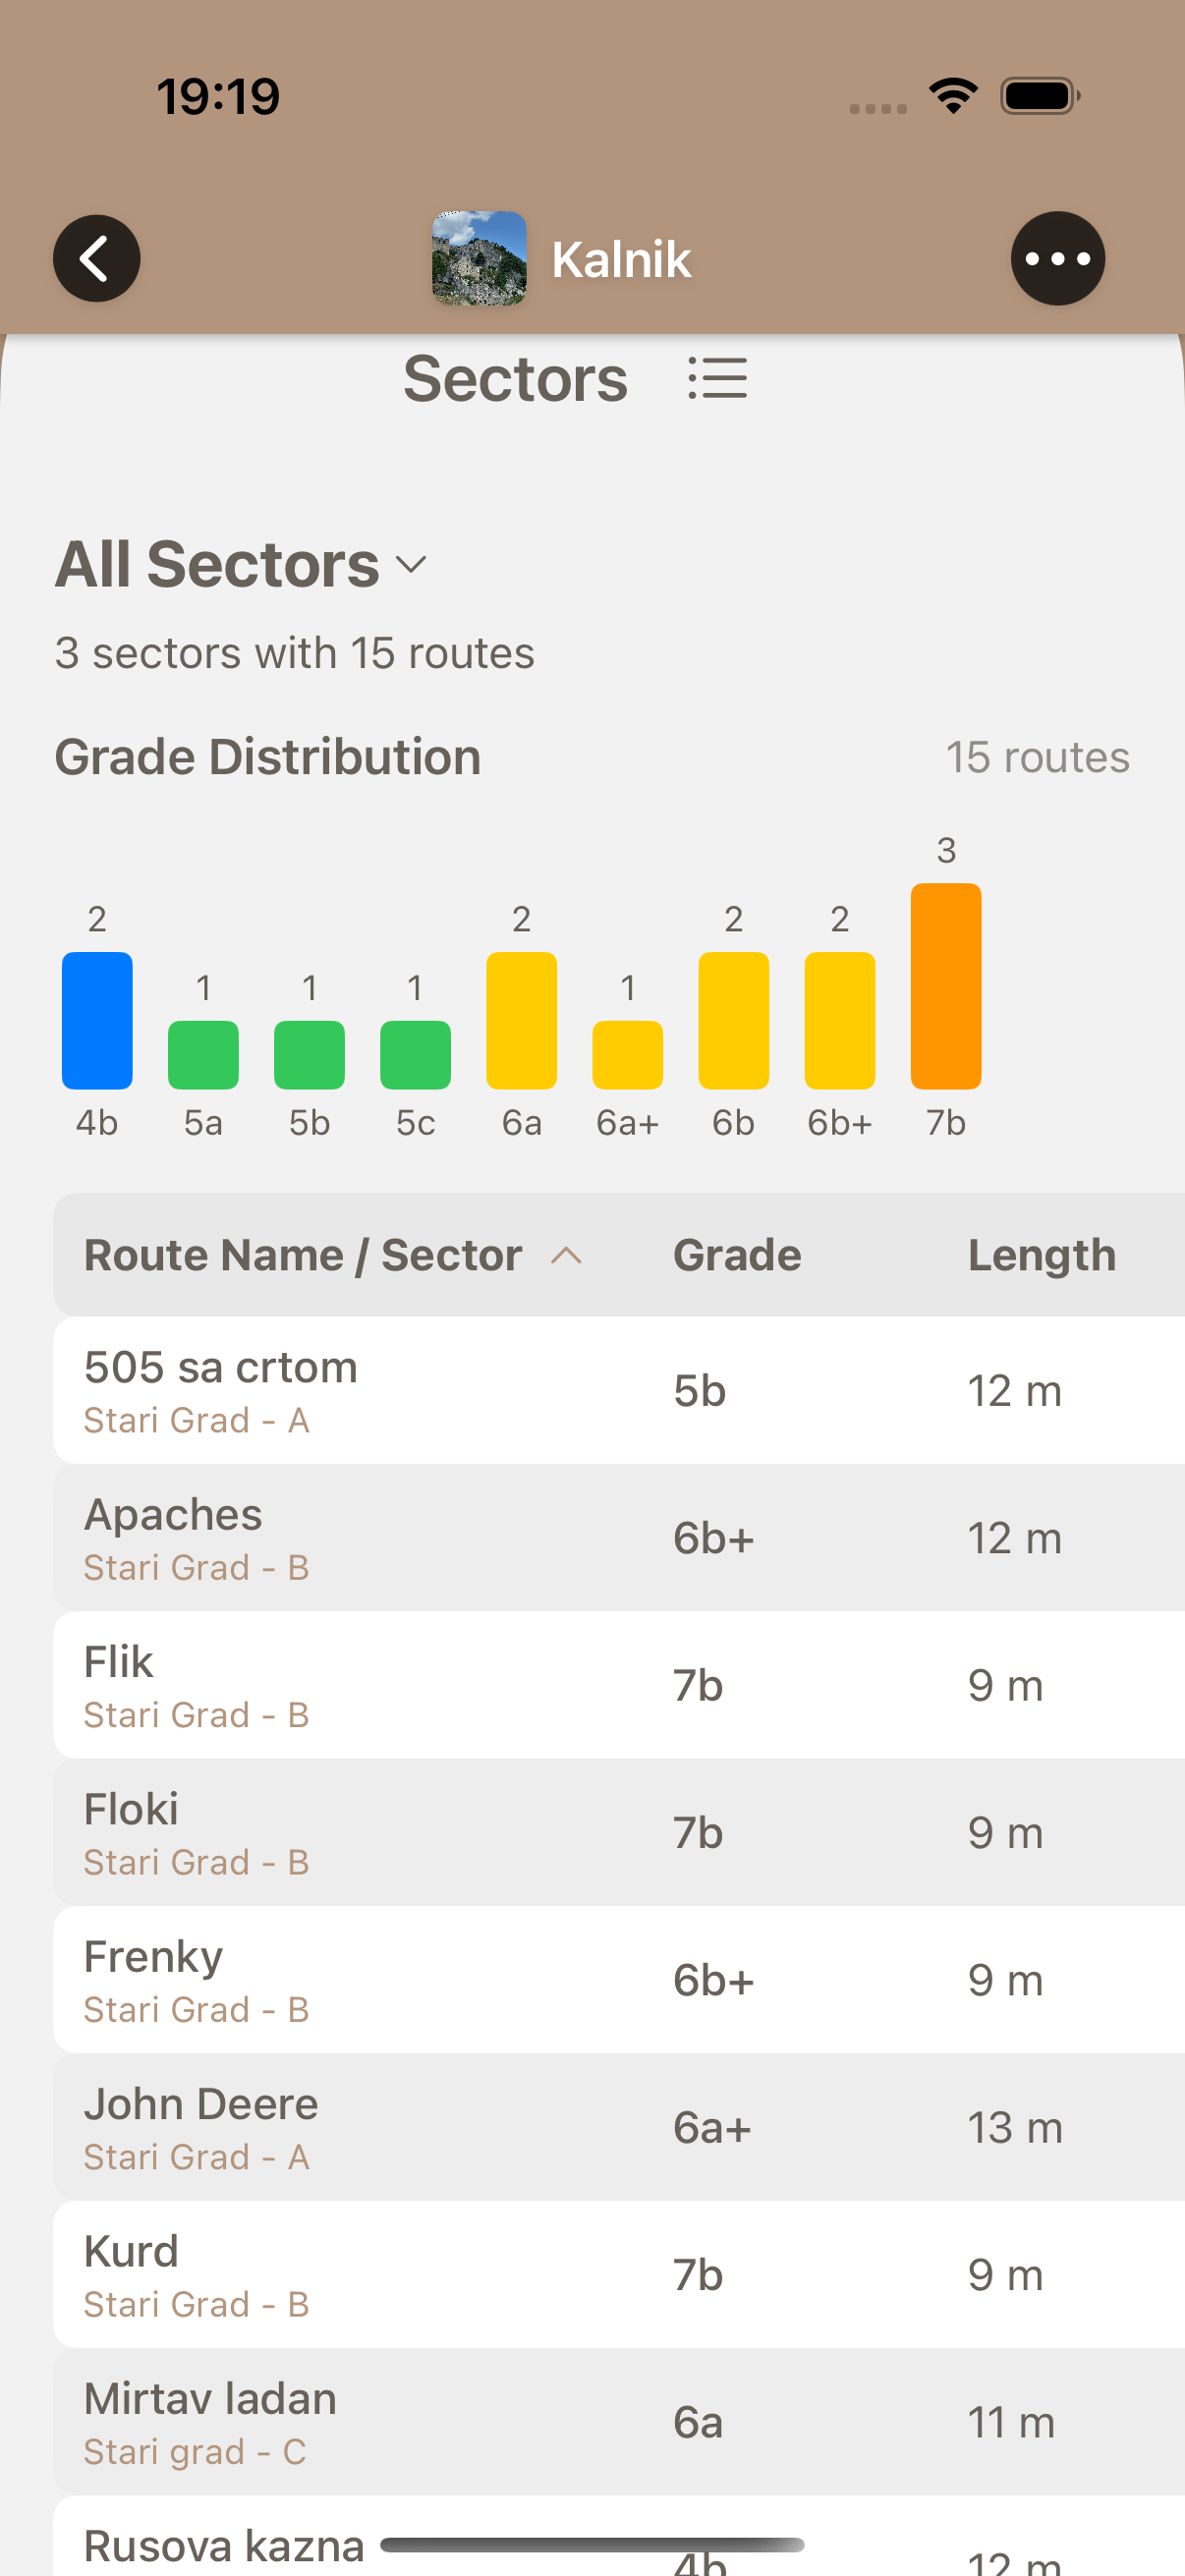
\includegraphics[width=0.35\textwidth]{images/implementacija/crag-details/crag-all-sectors-table.png}
    \caption{Tablični prikaz sektora na mobilnoj aplikaciji}
    \label{fig:tablični_prikaz_sektora}
\end{figure}

Ako korisnik preferira tablični prikaz na mobilnoj aplikaciji, može to promijeniti klikom na gumb pored naslova "Sektori" (eng. \textit{Sectors}) (slika~\ref{fig:tablični_prikaz_sektora}). Na web aplikaciji tablični prikaz je zadani prikaz. Tablični prikaz omogućuje pregled svih penjačkih smjerova te sortiranje po nazivu, težini, dužini, tipu te broju uspona. S obzirom da na web aplikaciji nije grupiran prikaz po sektorima, postoje filteri koji korisnik može koristiti za filtriranje penjačkih smjerova po imenu, tipu i sektoru.

Klikom na izbornik "Svi sektori" (eng. \textit{All sectors}) korisniku prikazuje se popis svih sektora na penjalištu (slika~\ref{fig:prikaz_detalja_za_odabrani_sektor}). 

\begin{figure}[H]
    \centering
    \begin{subfigure}[b]{0.35\textwidth}
        \centering
        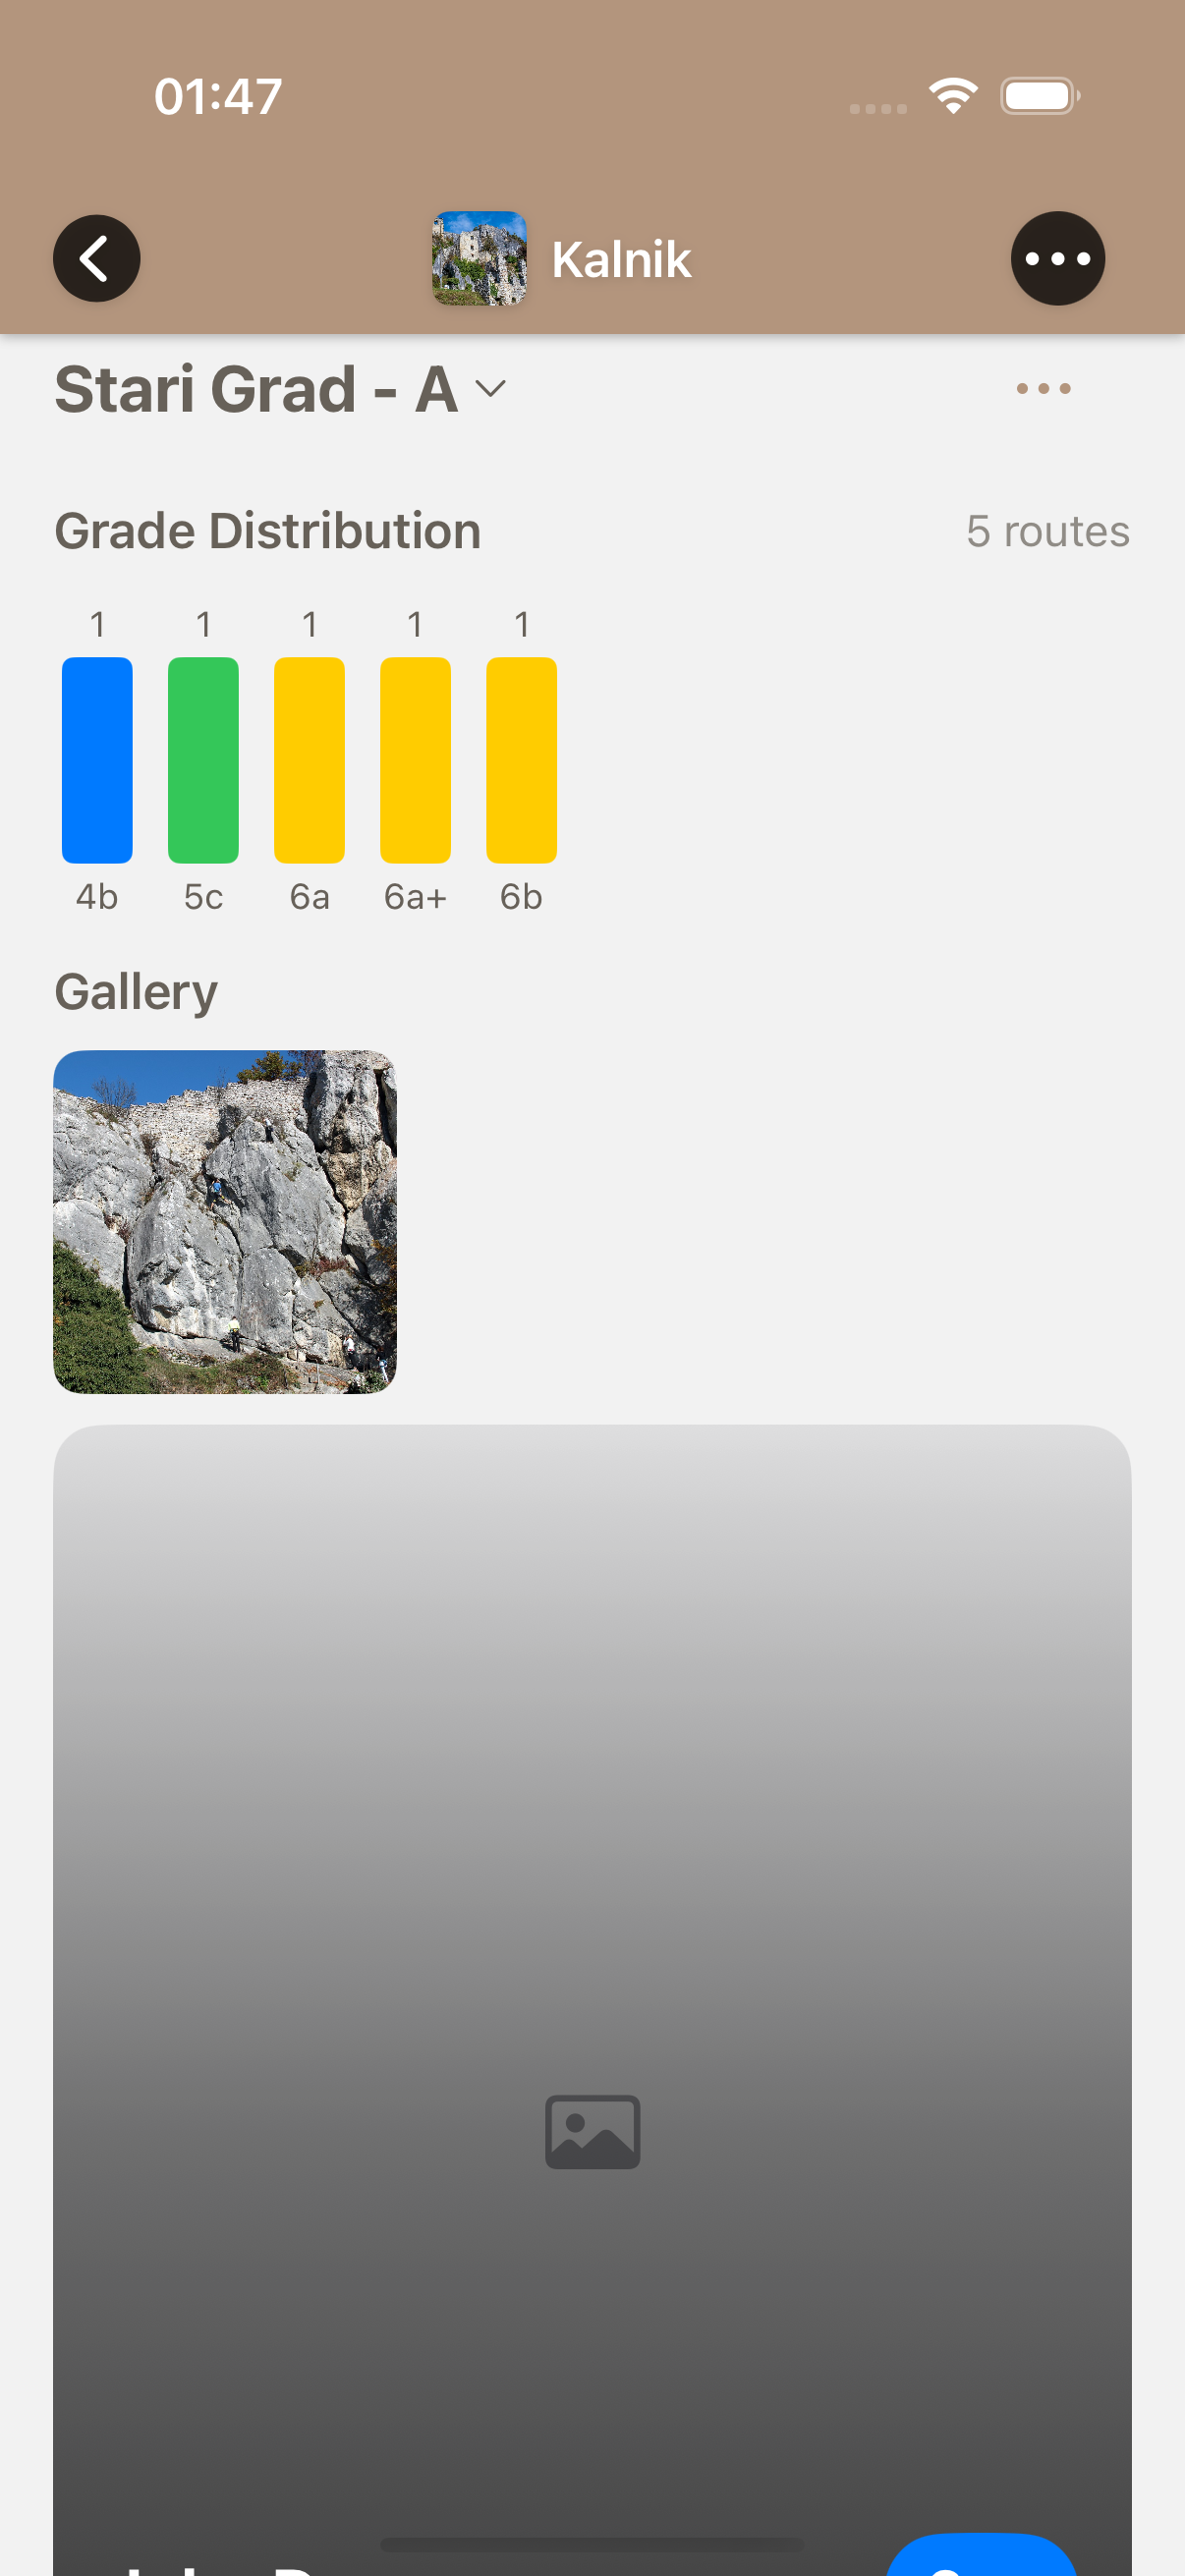
\includegraphics[width=\textwidth]{images/implementacija/crag-details/crag-selected-sector.png}
        \caption{Mobilna aplikacija}
        \label{fig:prikaz_detalja_za_odabrani_sektor_mob}
    \end{subfigure}
    \hfill
    \begin{subfigure}[b]{0.6\textwidth}
        \centering
        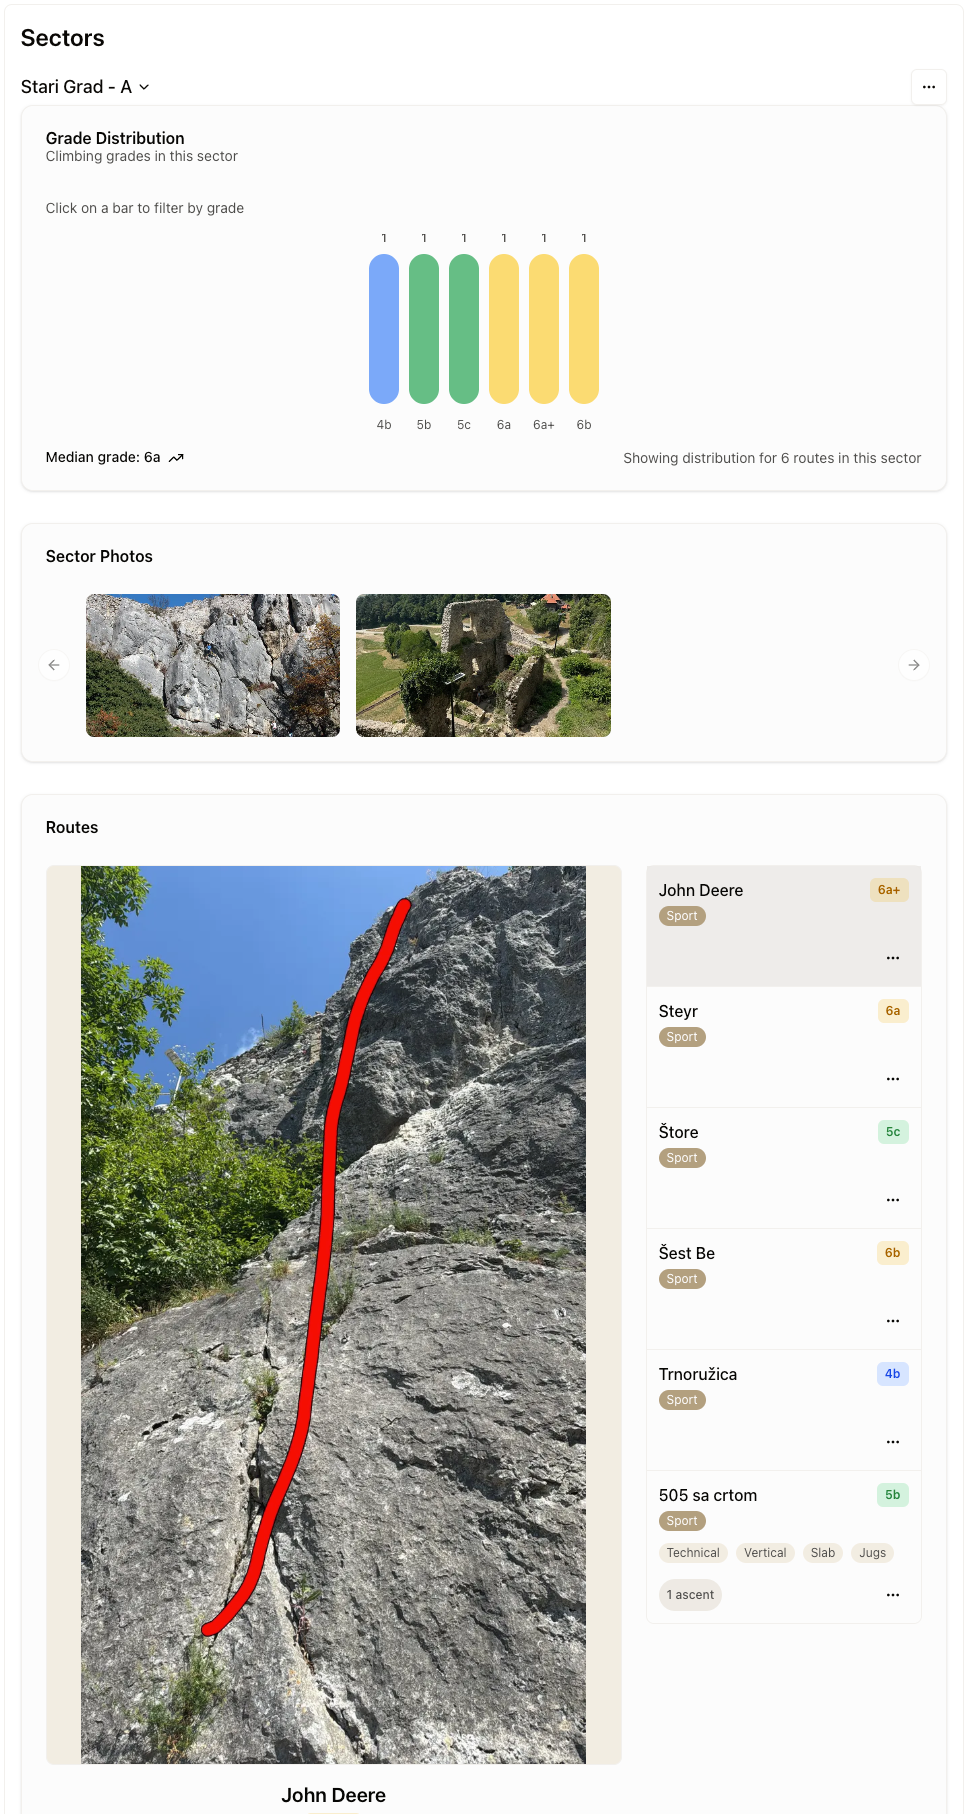
\includegraphics[width=1\textwidth]{images/implementacija/web/crag-details/crag-selected-sector.png}
        \caption{Web aplikacija}
        \label{fig:prikaz_detalja_za_odabrani_sektor_web}
    \end{subfigure}
    \caption{Prikaz detalja za odabrani sektor}
    \label{fig:prikaz_detalja_za_odabrani_sektor}
\end{figure}

Odabirom određenog sektora, korisniku se prikazuje graf težina filtriran po odabranom sektoru, slike sektora te popis svih penjačkih smjerova u tom sektoru. Klikom na određeni stupac na grafu težina, popis penjačkih smjerova se filtrira po označenoj težini. Tablični prikaz je isto dostupan klikom na gumb pored naslova "Sektori" (eng. \textit{Sectors}). Na web aplikaciji nalaze se ista funkcionalnost, ali s različitim prikazom.




% \section{Detalji penjačkog smjera}
% \section{Prepoznavanje penjačkih smjerova}

TODO: Nedostaju slike

Središnja funkcionalnost aplikacije i prednost u odnosu na postojeća rješenja jest funkcionalnost prepoznavanja i vizualizacije penjačkih smjerova u stvarnom vremenu. Ova mogućnost je dostupna samo u sklopu mobilne aplikacije i direkno rješava problem interpretacije 2D \textit{topo} slika. Pristup ovoj funkcionalnosti omogućen je sa zaslona s detaljnim pregledom penjačkog smjera. Odabirom opcije za prepozavanje, aplikacija aktivira kameru uređaja i pokreće proces temeljen na algoritmima rečunalnog vida. Korisnik usmjerava kameru prema stijeni, a aplikacija u pozadini kontinuirano analizira dobivene slike. Kada je prepoznat penjački smjer korisnik na svom ekranu vidi stvarni svijet s virtualnom linijom koja je nacrtana na stijeni označavajući točnu liniju penjačkog smjera.

Aplikacija nudi korisniku postavke za prilagodbu procesa prepozavanja. Korisnik može birati između dva glavna načina rada. U automatskom načinu rada (eng. \textit{Automatic mode}), aplikacija kontinuirano analizira slike dobivene s kamere i automatski pokušava prepoznati smjer što pruži iskustvo proširene stvarnosti. 

S obzirom na računalno intezivnu prirodu tog procesa, kao alternativu kako bi se smanjila potrošnja resursa, dostupan je i ručni način rada (eng. \textit{Manual mode}). U tom načinu rada, aplikacija ne analizira slike u realnom vremenu, već korisnik samostalno snima fotografiju stijene, a proces prepoznavanja se izvršava samo na toj jednoj, statičnoj slici. 

Dodatno, korisniku su na raspolaganju dostupne i tri razine jačine prepozavanja: \textit{Low}, \textit{Medium} i \textit{High}. Ove postavke u pozadini prilagođavaju parametre algoritama kako bi se postigao kompromis između brzine i kvalitete prepoznavanja. Viša razina jačine prepoznavanja rezultira u preciznijim prepoznavanjima, ali uz veće računsko opterećenje, dok niža nudi brži rad i manju potrošnju. Ove opcije omogućuju korisniku da prilagodi proces prepozavanja prema svojim potrebama i uvjetima.
% \section{Korisnički profil}

Svaki registrirani korisnik unutar aplikacije ima pregled profila koji služi kao centralno mjesto za pregled svih njegovih penjačkih aktivnosti i analizu napretka. Pristupom profilu korisniku se prikazuje sažetak njegovih penjačkih aktivnosti poput ukupnog broja posjećenih penjališta, ukupan broj zabilježenih uspona te broj dodanih fotografija.

\begin{figure}[H]
    \centering
    \begin{subfigure}[b]{0.3\textwidth}
        \centering
        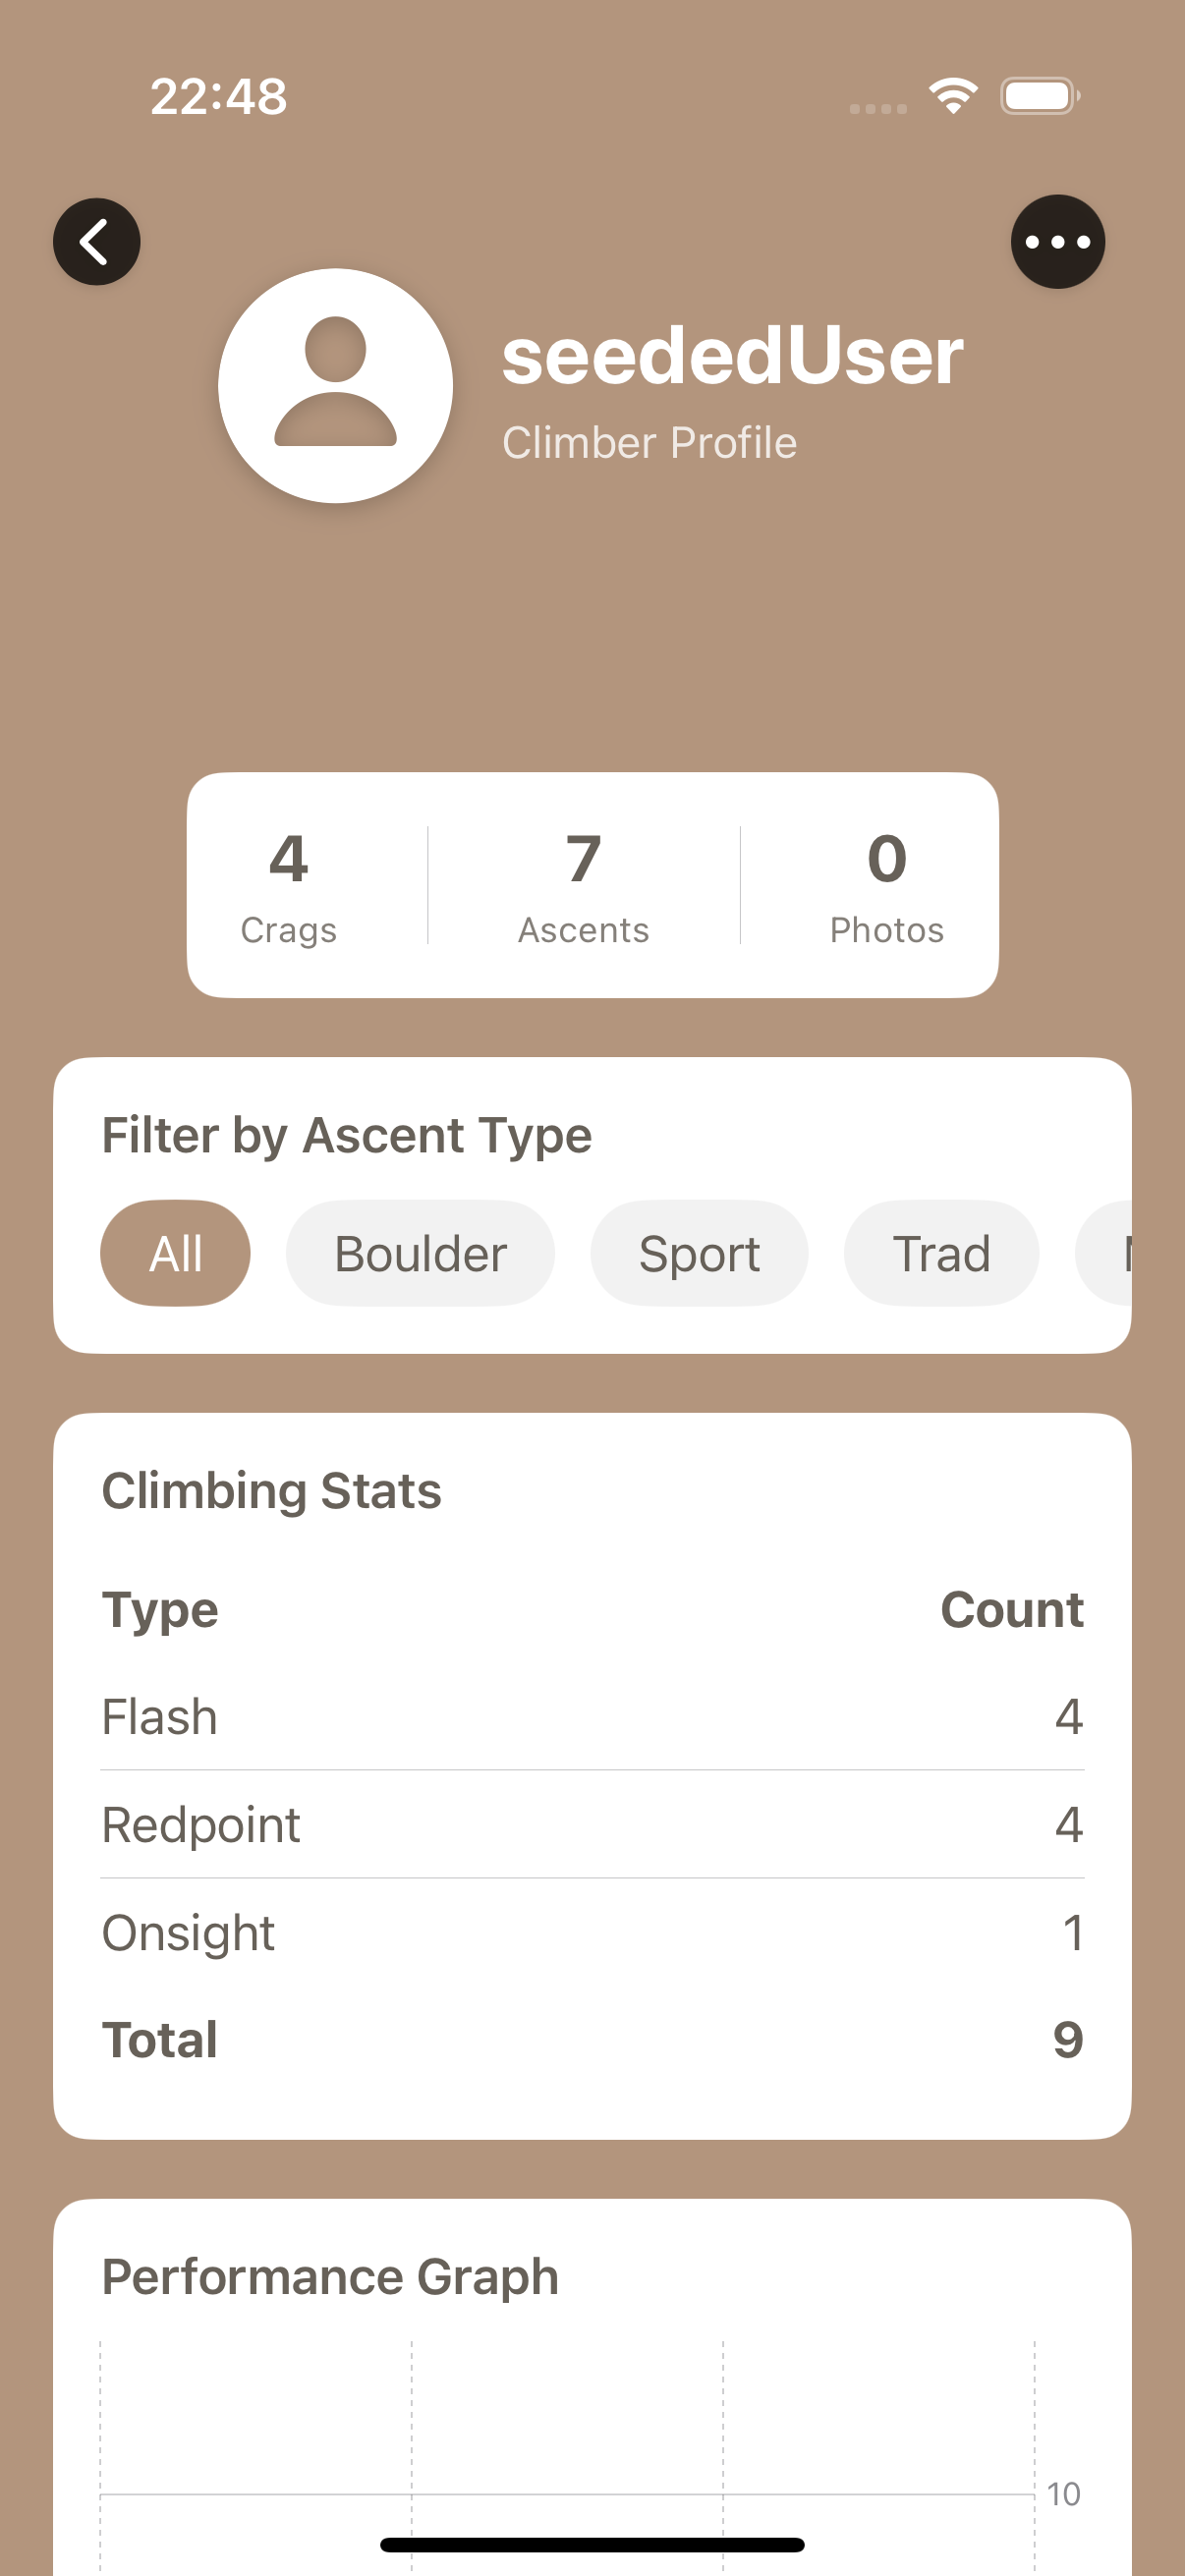
\includegraphics[width=\textwidth]{images/implementacija/user_profile_1.png}
        \caption{Mobilna aplikacija}
        \label{fig:korisnicki_profil_mob}
    \end{subfigure}
    \hfill
    \begin{subfigure}[b]{0.65\textwidth}
        \centering
        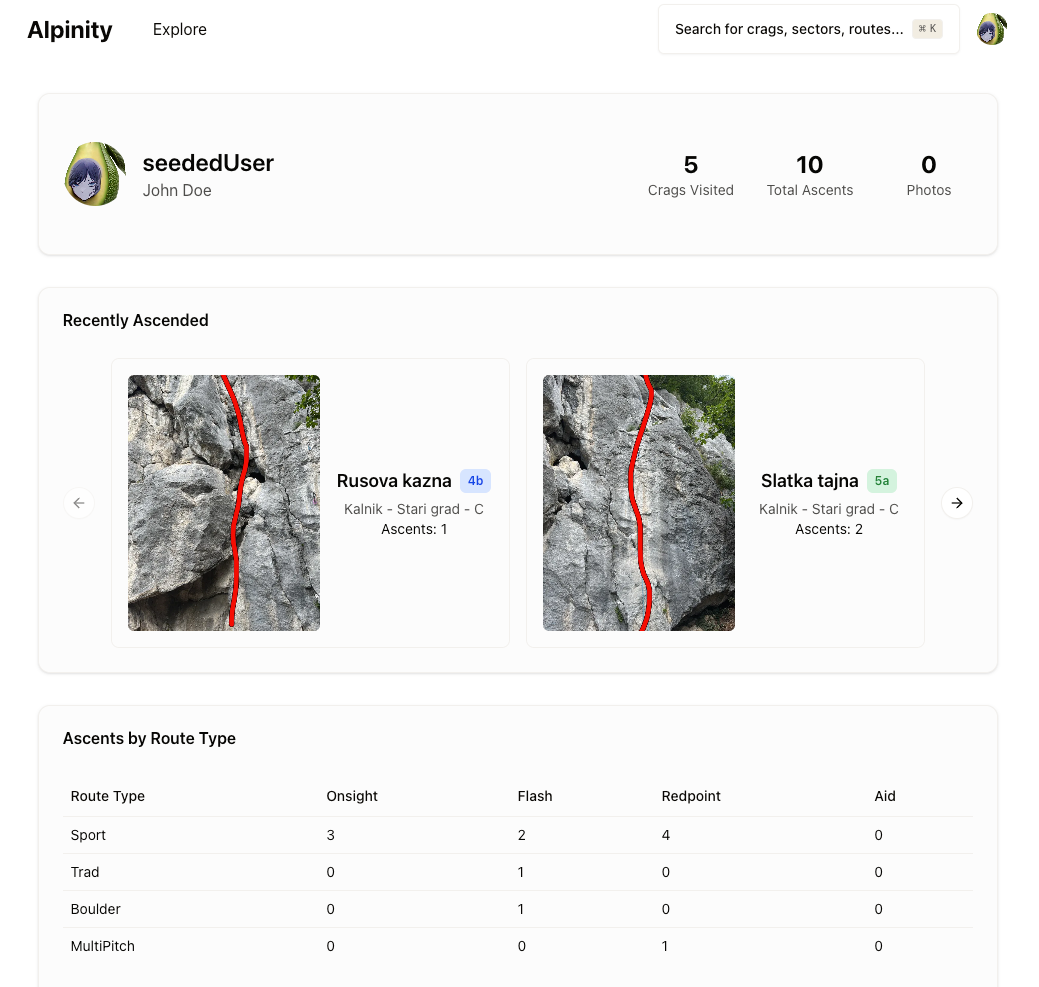
\includegraphics[width=\textwidth]{images/implementacija/web/user-profile-1.png}
        \caption{Web aplikacija}
        \label{fig:korisnicki_profil_web}
    \end{subfigure}
    \caption{Korisnički profil}
    \label{fig:korisnicki_profil}
\end{figure}

Središnji dio profila posvećen je detaljnoj statističkoj analizi (slika~\ref{fig:korisnicki_profil}). Korisnik može filtrirati svoje uspone prema penjačkoj disciplini, poput boulder, sportsko penjanje ili tradicionalno penjanje, kako bi dobio precizniji uvid u svoje aktivnosti. Aplikacija pruža tablični prikaz broja uspona po stilu (Flash, Redpoint, Onsight), omogućujući korisniku da lako vidi koje stilove najčešće prakticira. Dodatno web aplikacija sadrži i nedavno popete penjačke smjerove za korisnika organizirane u horizontalnoj listi sortiranim po datumu uspona od najnovije prema najstarijem.

\begin{figure}[H]
    \centering
    \begin{subfigure}[b]{0.3\textwidth}
        \centering
        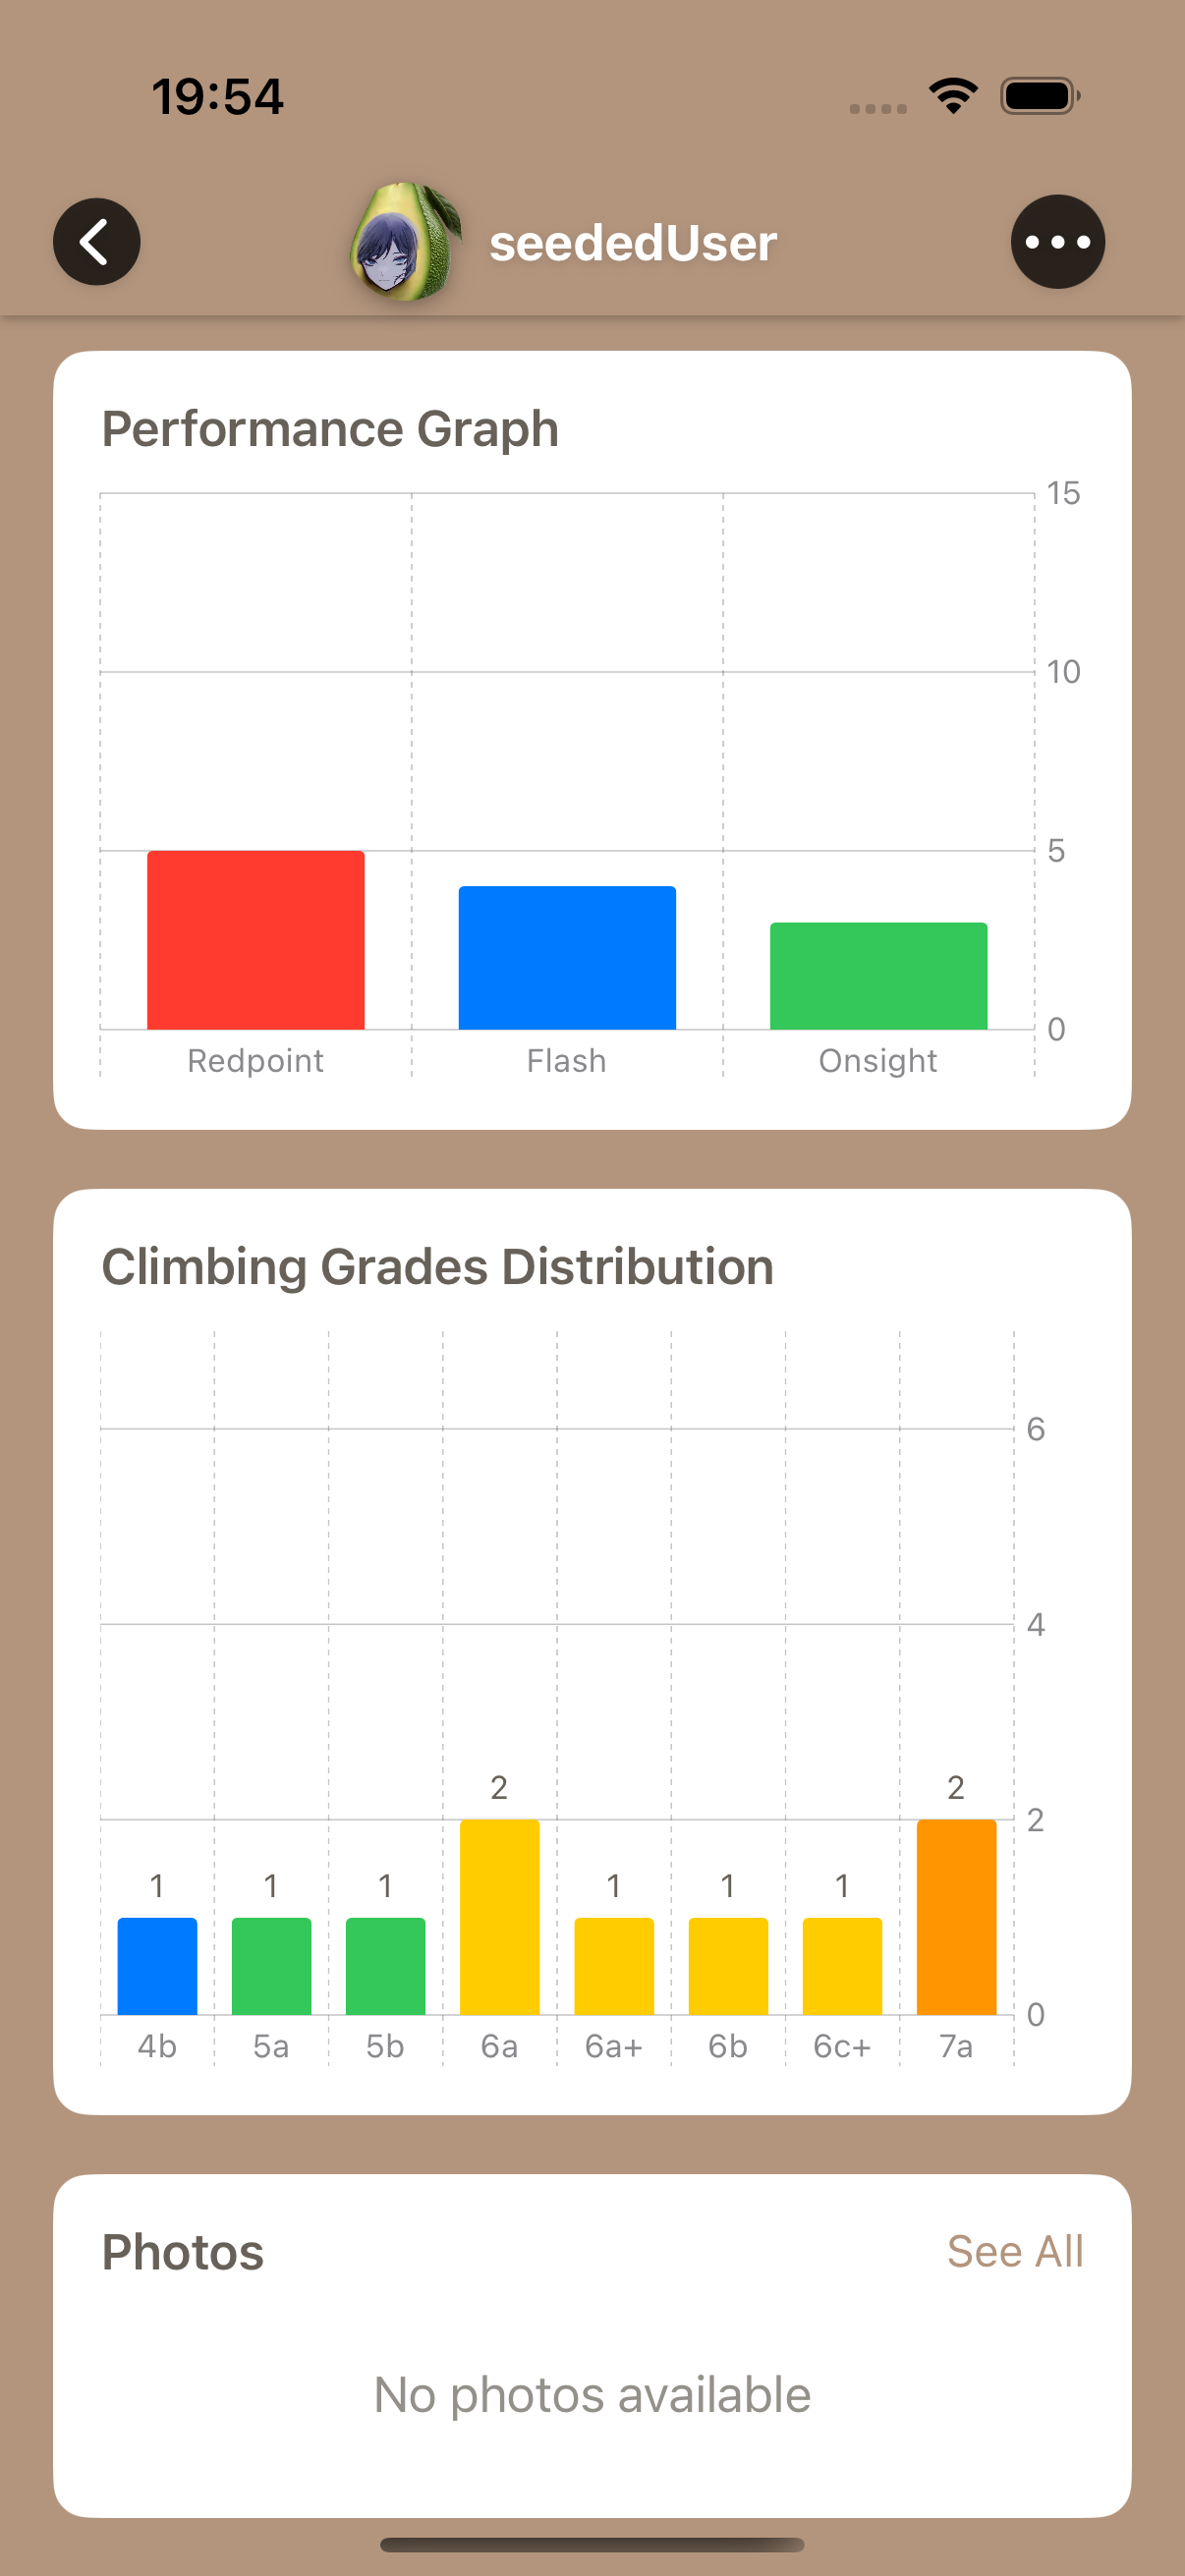
\includegraphics[width=\textwidth]{images/implementacija/user_profile_2.png}
        \caption{Mobilna aplikacija}
        \label{fig:korisnicki_profil_graf_mob}
    \end{subfigure}
    \hfill
    \begin{subfigure}[b]{0.65\textwidth}
        \centering
        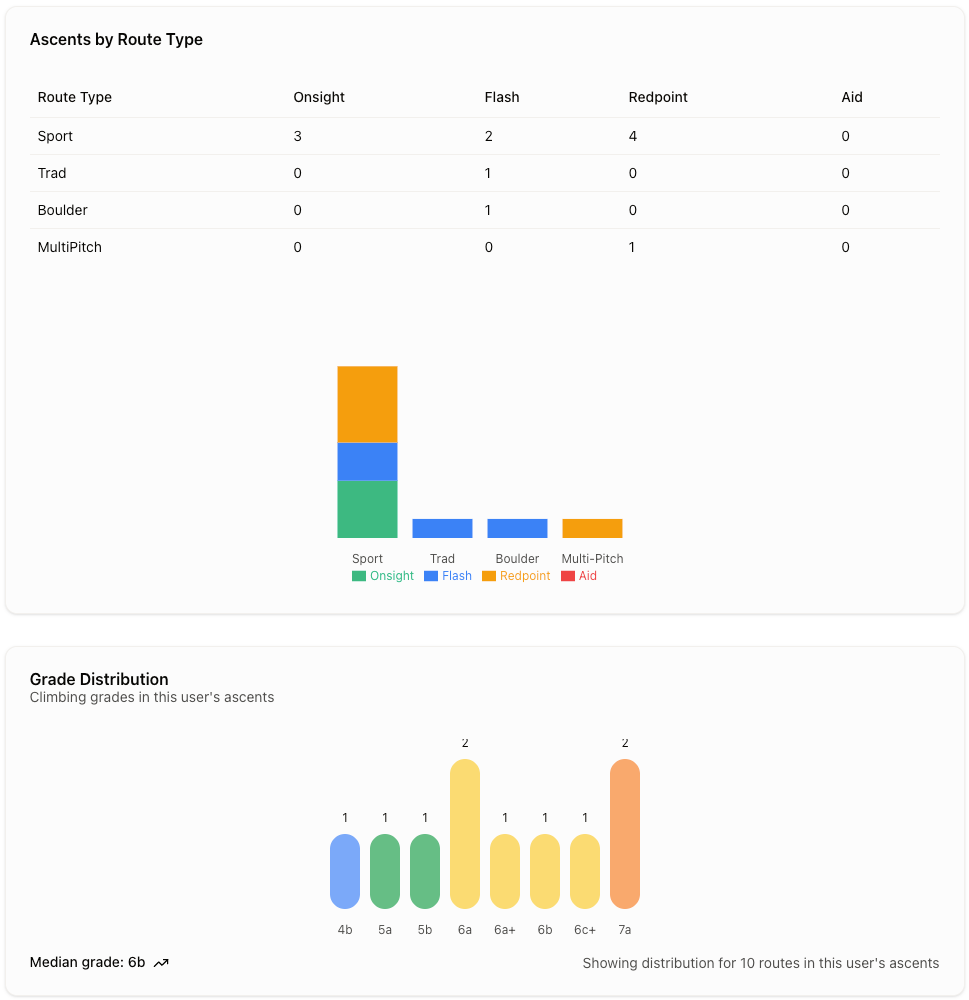
\includegraphics[width=\textwidth]{images/implementacija/web/user-profile-2.png}
        \caption{Web aplikacija}
        \label{fig:korisnicki_profil_graf_web}
    \end{subfigure}
    \caption{Grafovi performansi i distribucije po ocjenama}
    \label{fig:korisnicki_profil_2}
\end{figure}

Za bolju vizualizaciju, podaci su prikazani i u dva ključna grafa (slika~\ref{fig:korisnicki_profil_2}). Graf performansi prikazuje distribuciju uspona po stilu, dok graf distribucije po ocjenama prikazuje stupčastim diagramom, odnosno koliko je penjačkih smjerova određene težine je korisnik uspješno popeo. Ovi grafički prikazi omogućuju procjenu vlastitih sposobnosti i napretka tokom vremena. Finalno na dnu profila nalazi se i lista svih slika kojima korisnik želi istaknuti svoj profil.

\begin{figure}[H]
    \centering
    \begin{subfigure}[b]{0.33\textwidth}
        \centering
        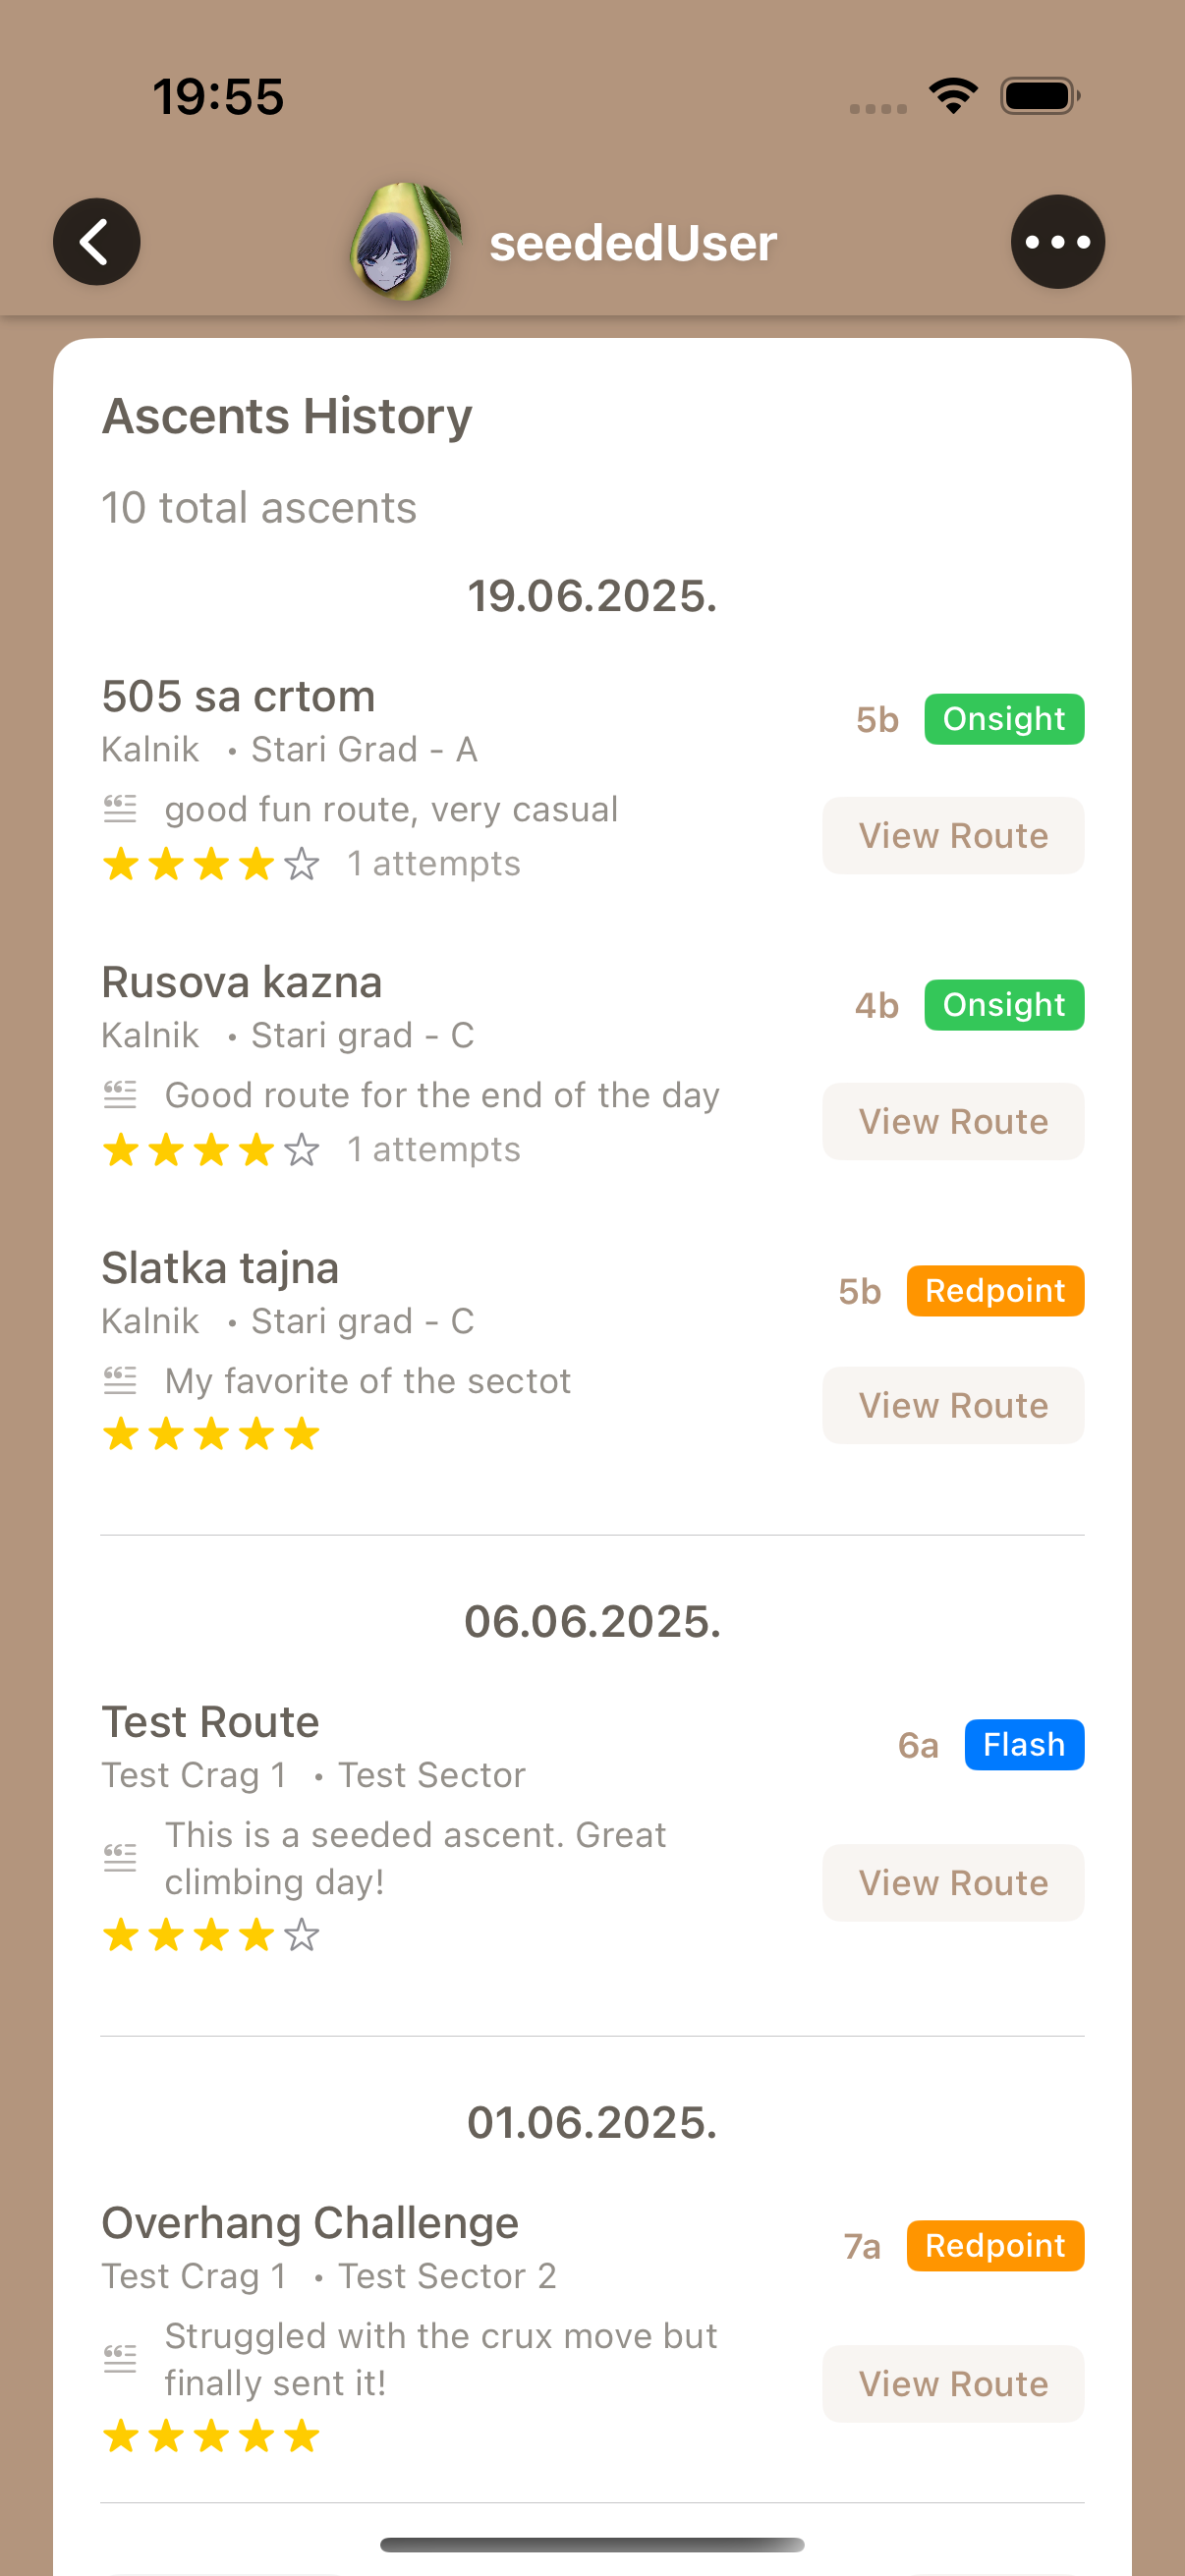
\includegraphics[width=\textwidth]{images/implementacija/user_profile_3.png}
        \caption{Mobilna aplikacija}
        \label{fig:korisnicki_profil_povijest_mob}
    \end{subfigure}
    \hfill
    \begin{subfigure}[b]{0.65\textwidth}
        \centering
        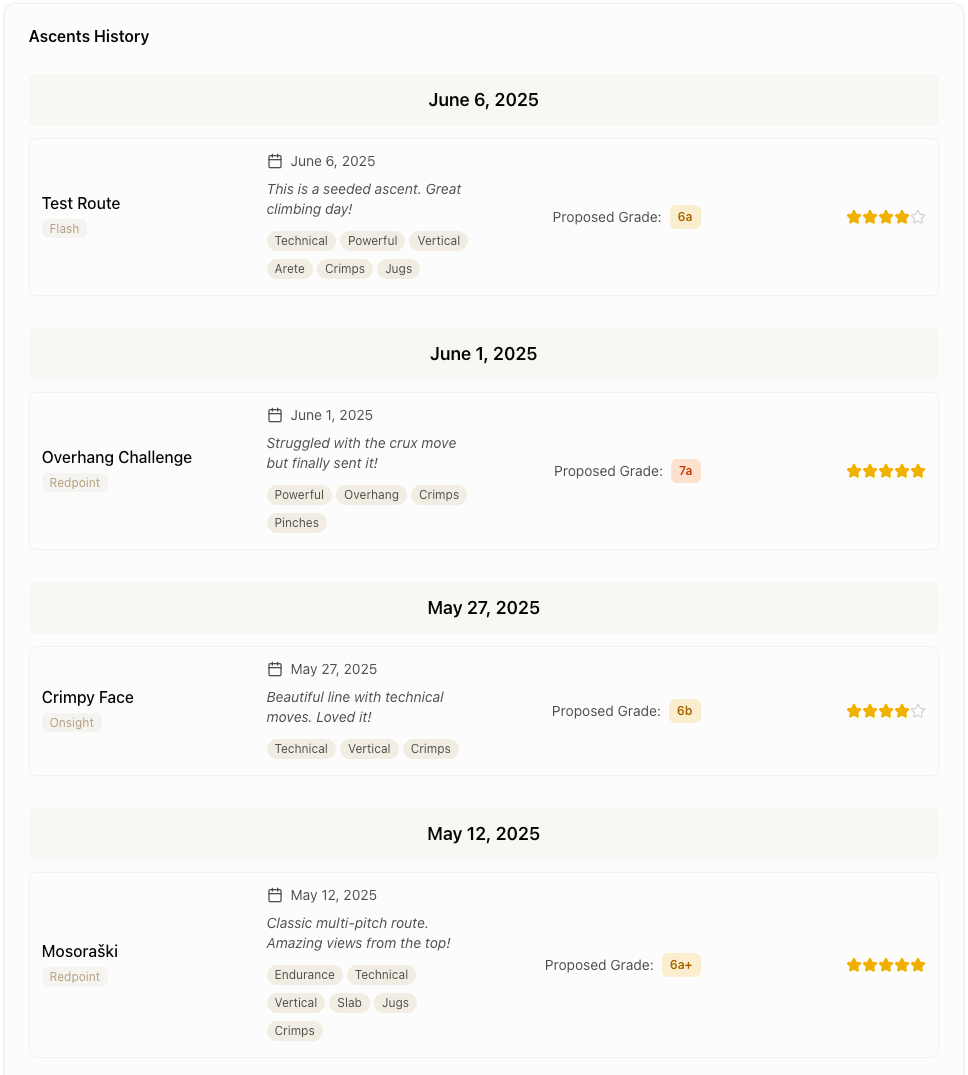
\includegraphics[width=\textwidth]{images/implementacija/web/user-profile-3.png}
        \caption{Web aplikacija}
        \label{fig:korisnicki_profil_povijest_web}
    \end{subfigure}
    \caption{Povijest uspona}
    \label{fig:korisnički_profil_3}
\end{figure}

Osim statistike, profil sadrži i povijest svih uspona, kronološki poredanih od najnovijeg prema najstarijem (slika~\ref{fig:korisnički_profil_3}). Svaki unos u povijest sadrži sve relevantne informacije poput datuma, naziva penjačkog smjera, lokaciju, težinu, stil uspona, osobni komentar i ocjenu smjera te direktnu poveznicu na detaljni pregled samog penjačkog smjera. Ovaj dnevnik služi kao vrijedan alat za prisjećanje na prethodna penjačka iskustva.

\subsection{Korisnički profil drugog korisnika}

Pretraživanjem korisničkog profila drugog korisnika, korisnik može vidjeti statistike, grafove performansi i povijest uspona drugog korisnika na isti način kao i na vlastitom profilu (slika~\ref{fig:korisnički_profil_other}).


\begin{figure}[H]
    \centering
    \begin{subfigure}[b]{0.33\textwidth}
        \centering
        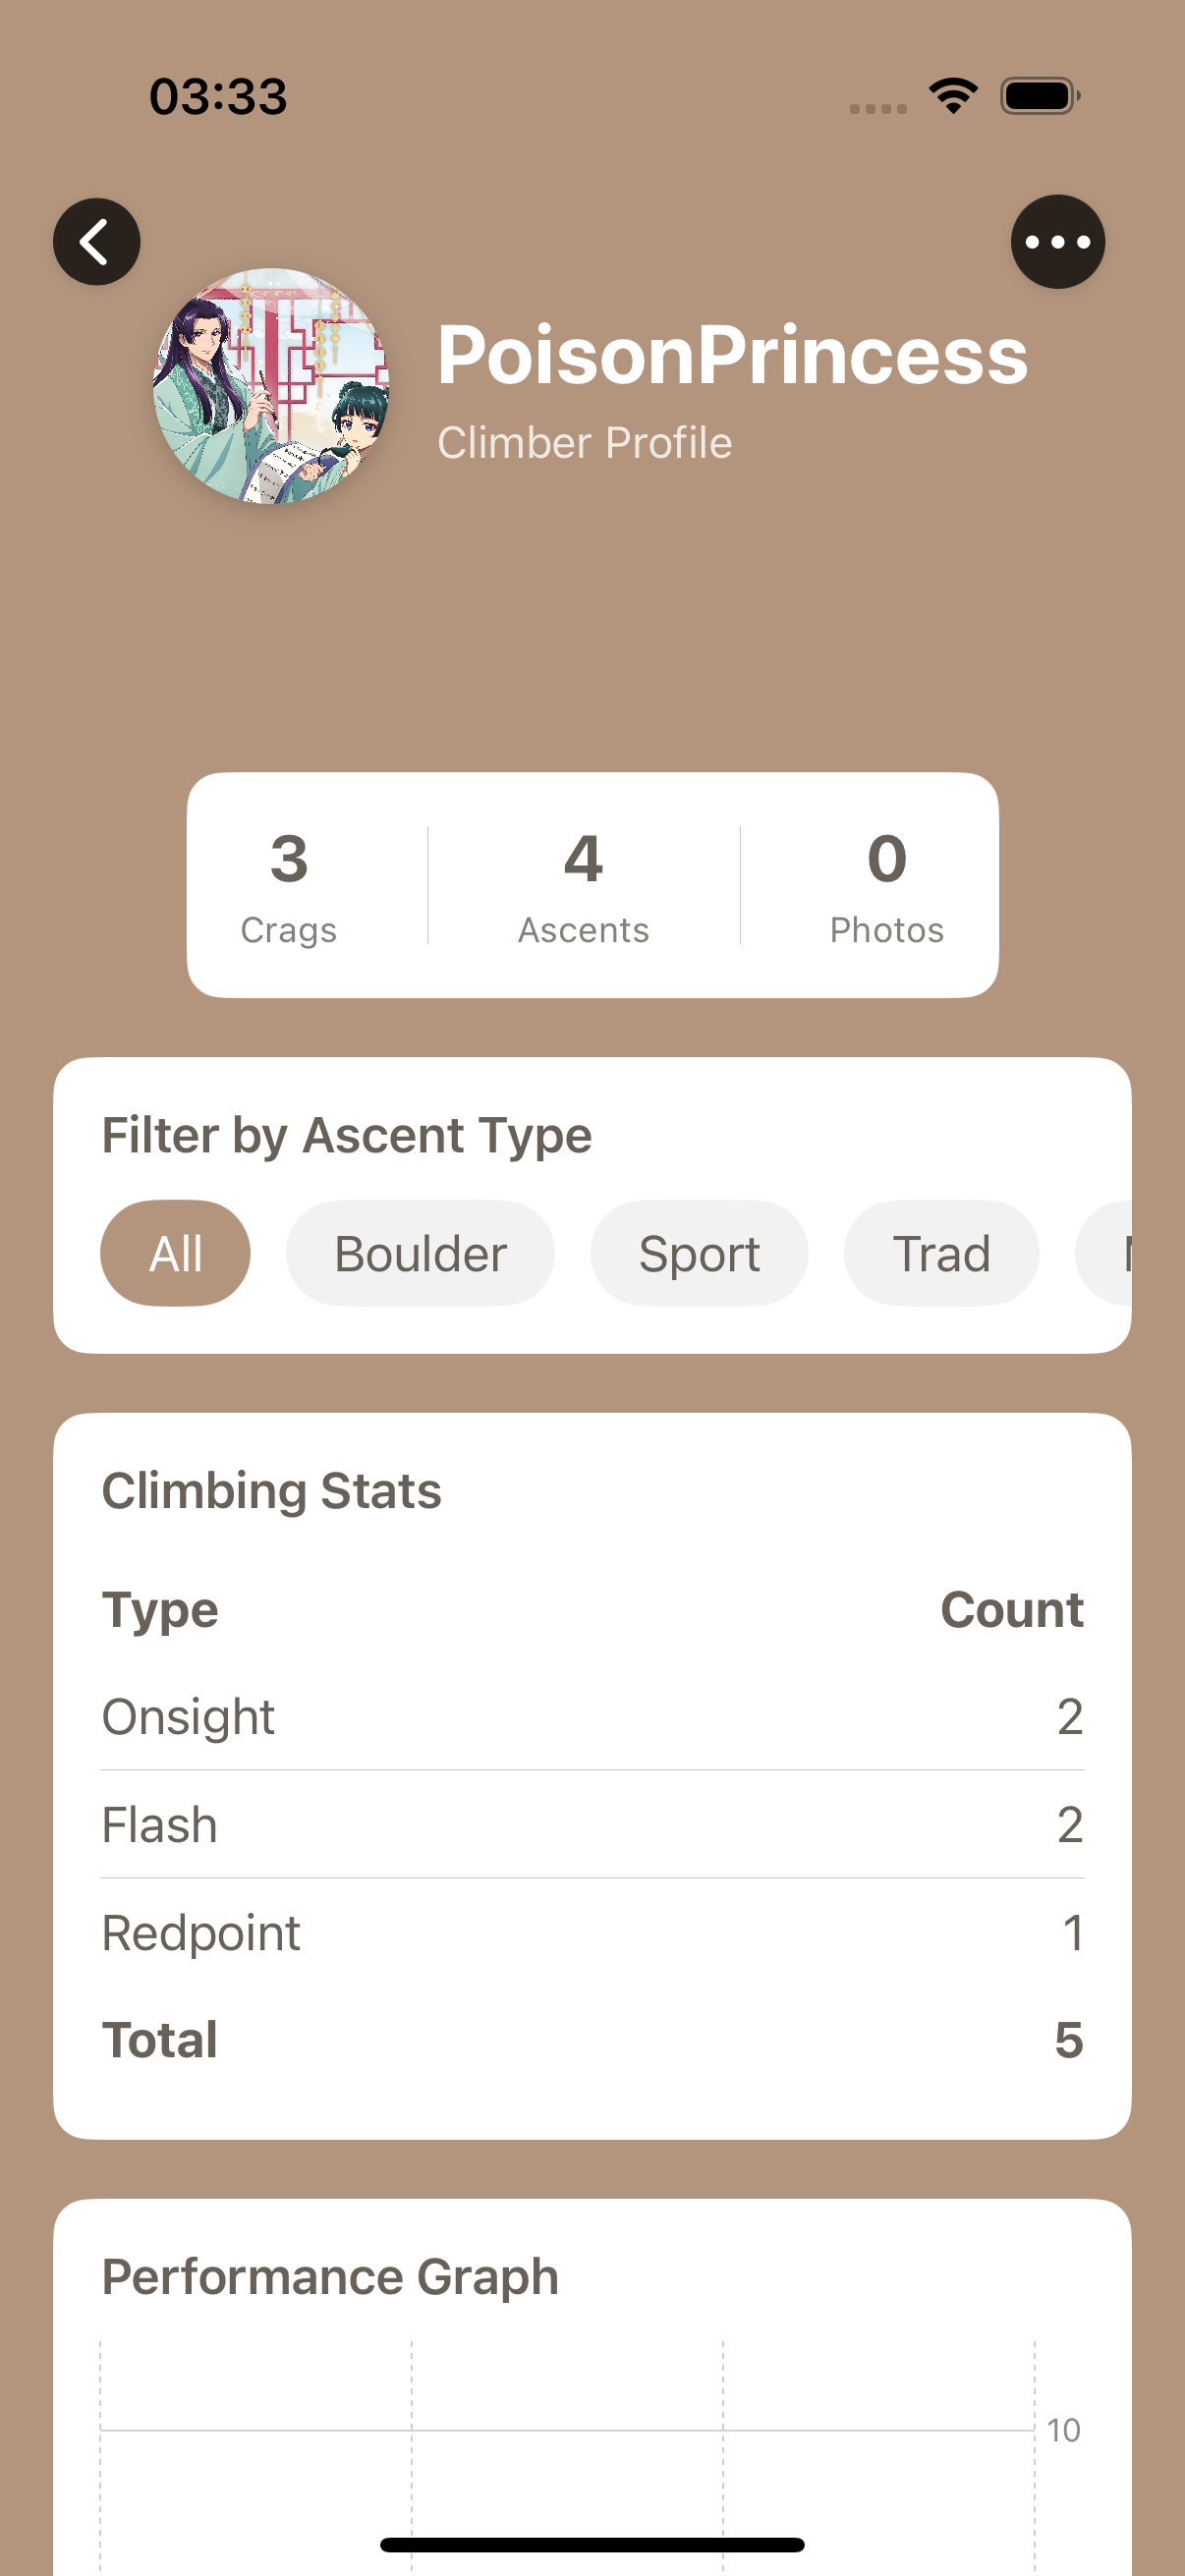
\includegraphics[width=\textwidth]{images/implementacija/user-profile-other.png}
        \caption{Mobilna aplikacija}
        \label{fig:korisnicki_profil_other_mob}
    \end{subfigure}
    \hfill
    \begin{subfigure}[b]{0.65\textwidth}
        \centering
        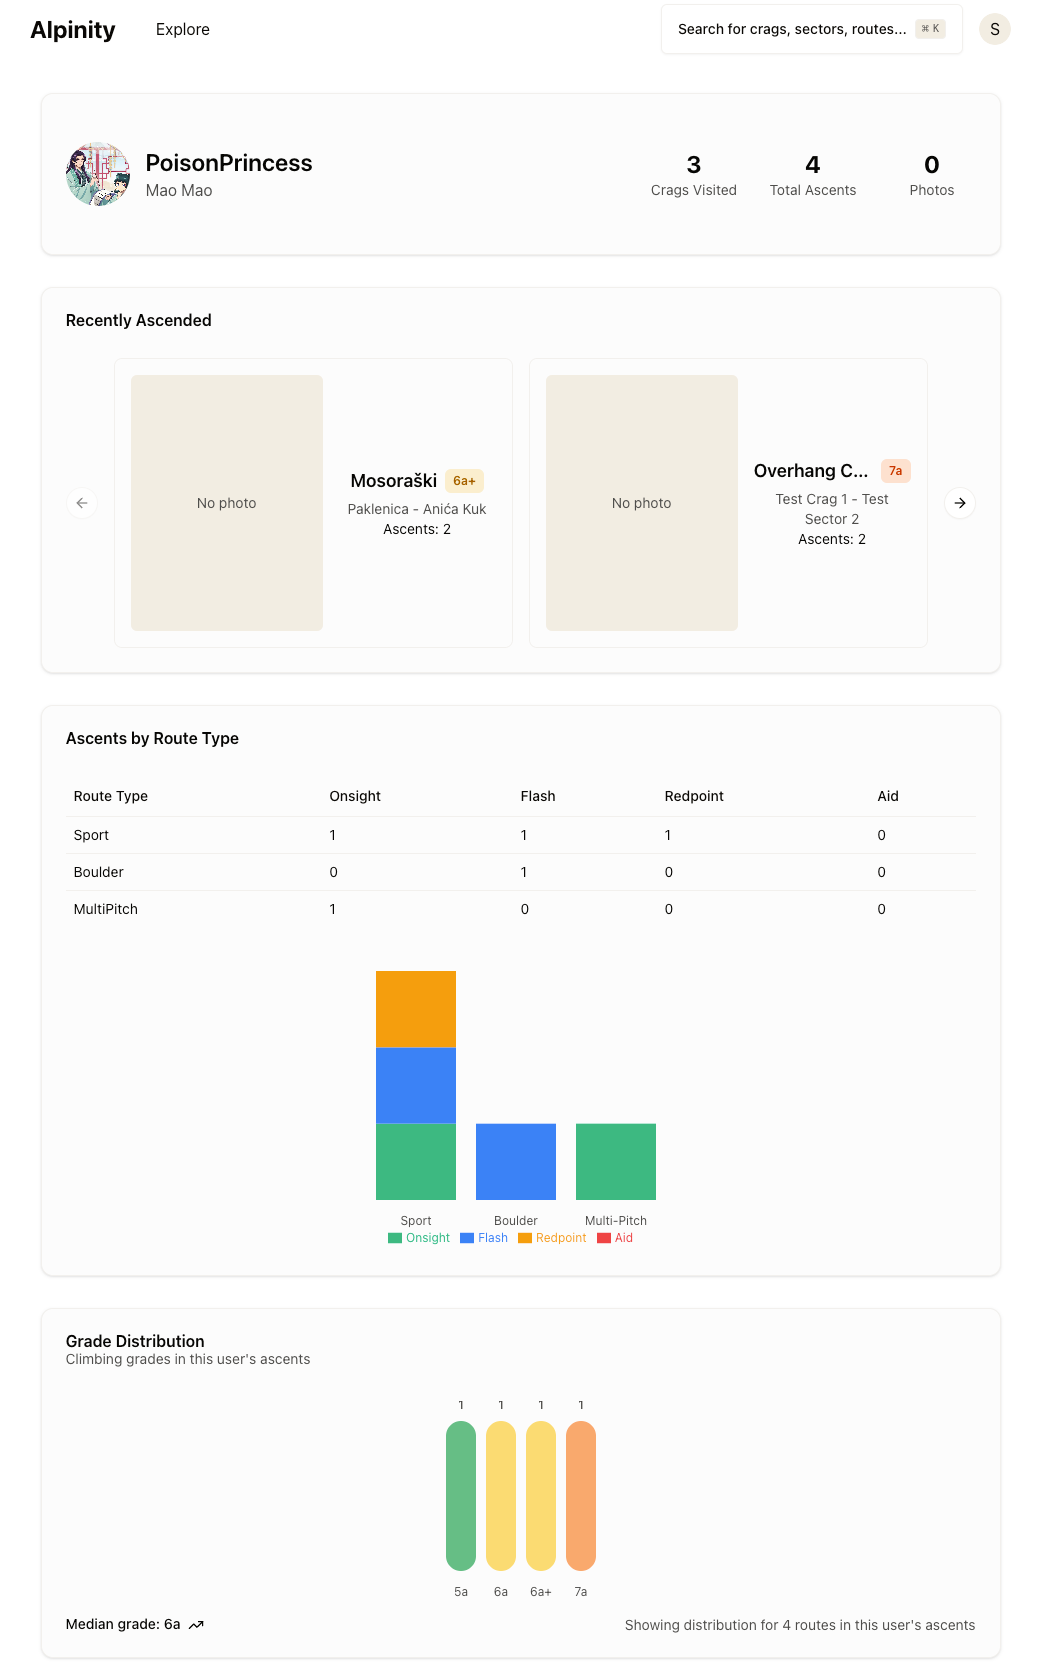
\includegraphics[width=\textwidth]{images/implementacija/web/user-profile-other.png}
        \caption{Web aplikacija}
        \label{fig:korisnicki_profil_other_web}
    \end{subfigure}
    \caption{Korisnički profil drugog korisnika}
    \label{fig:korisnički_profil_other}
\end{figure}

\section{Unos i uređivanje podataka}

Kako bi sustav bio dinamičan i ažuran, aplikacija omogućuje ovlaštenim korisnicima kreiranje i uređivanje svih hijerarhijskih razina podataka, od penjališta do pojedinačnih penjačkih smjerova.

\subsection{Dodavanje, uređivanje i brisanje penjališta}

Na korisničkom profilu omogućeno je kreiranje novog penjališta u izborniku u gornjem desnom kutu korisničkog profila. Na web aplikaciji ta opcija se nalazi u navigacijskoj traci u postavkama korisničkog izbornika. Funkcionalnost kreiranja novog penjališta nije dostupna svim korisnicima, već je ograničena na one s posebnim ovlastima, a to su administratori sustava i verificirani korisnici (eng. \textit{creators}). 

\begin{figure}[H]
    \centering
    \begin{subfigure}[b]{0.31\textwidth}
        \centering
        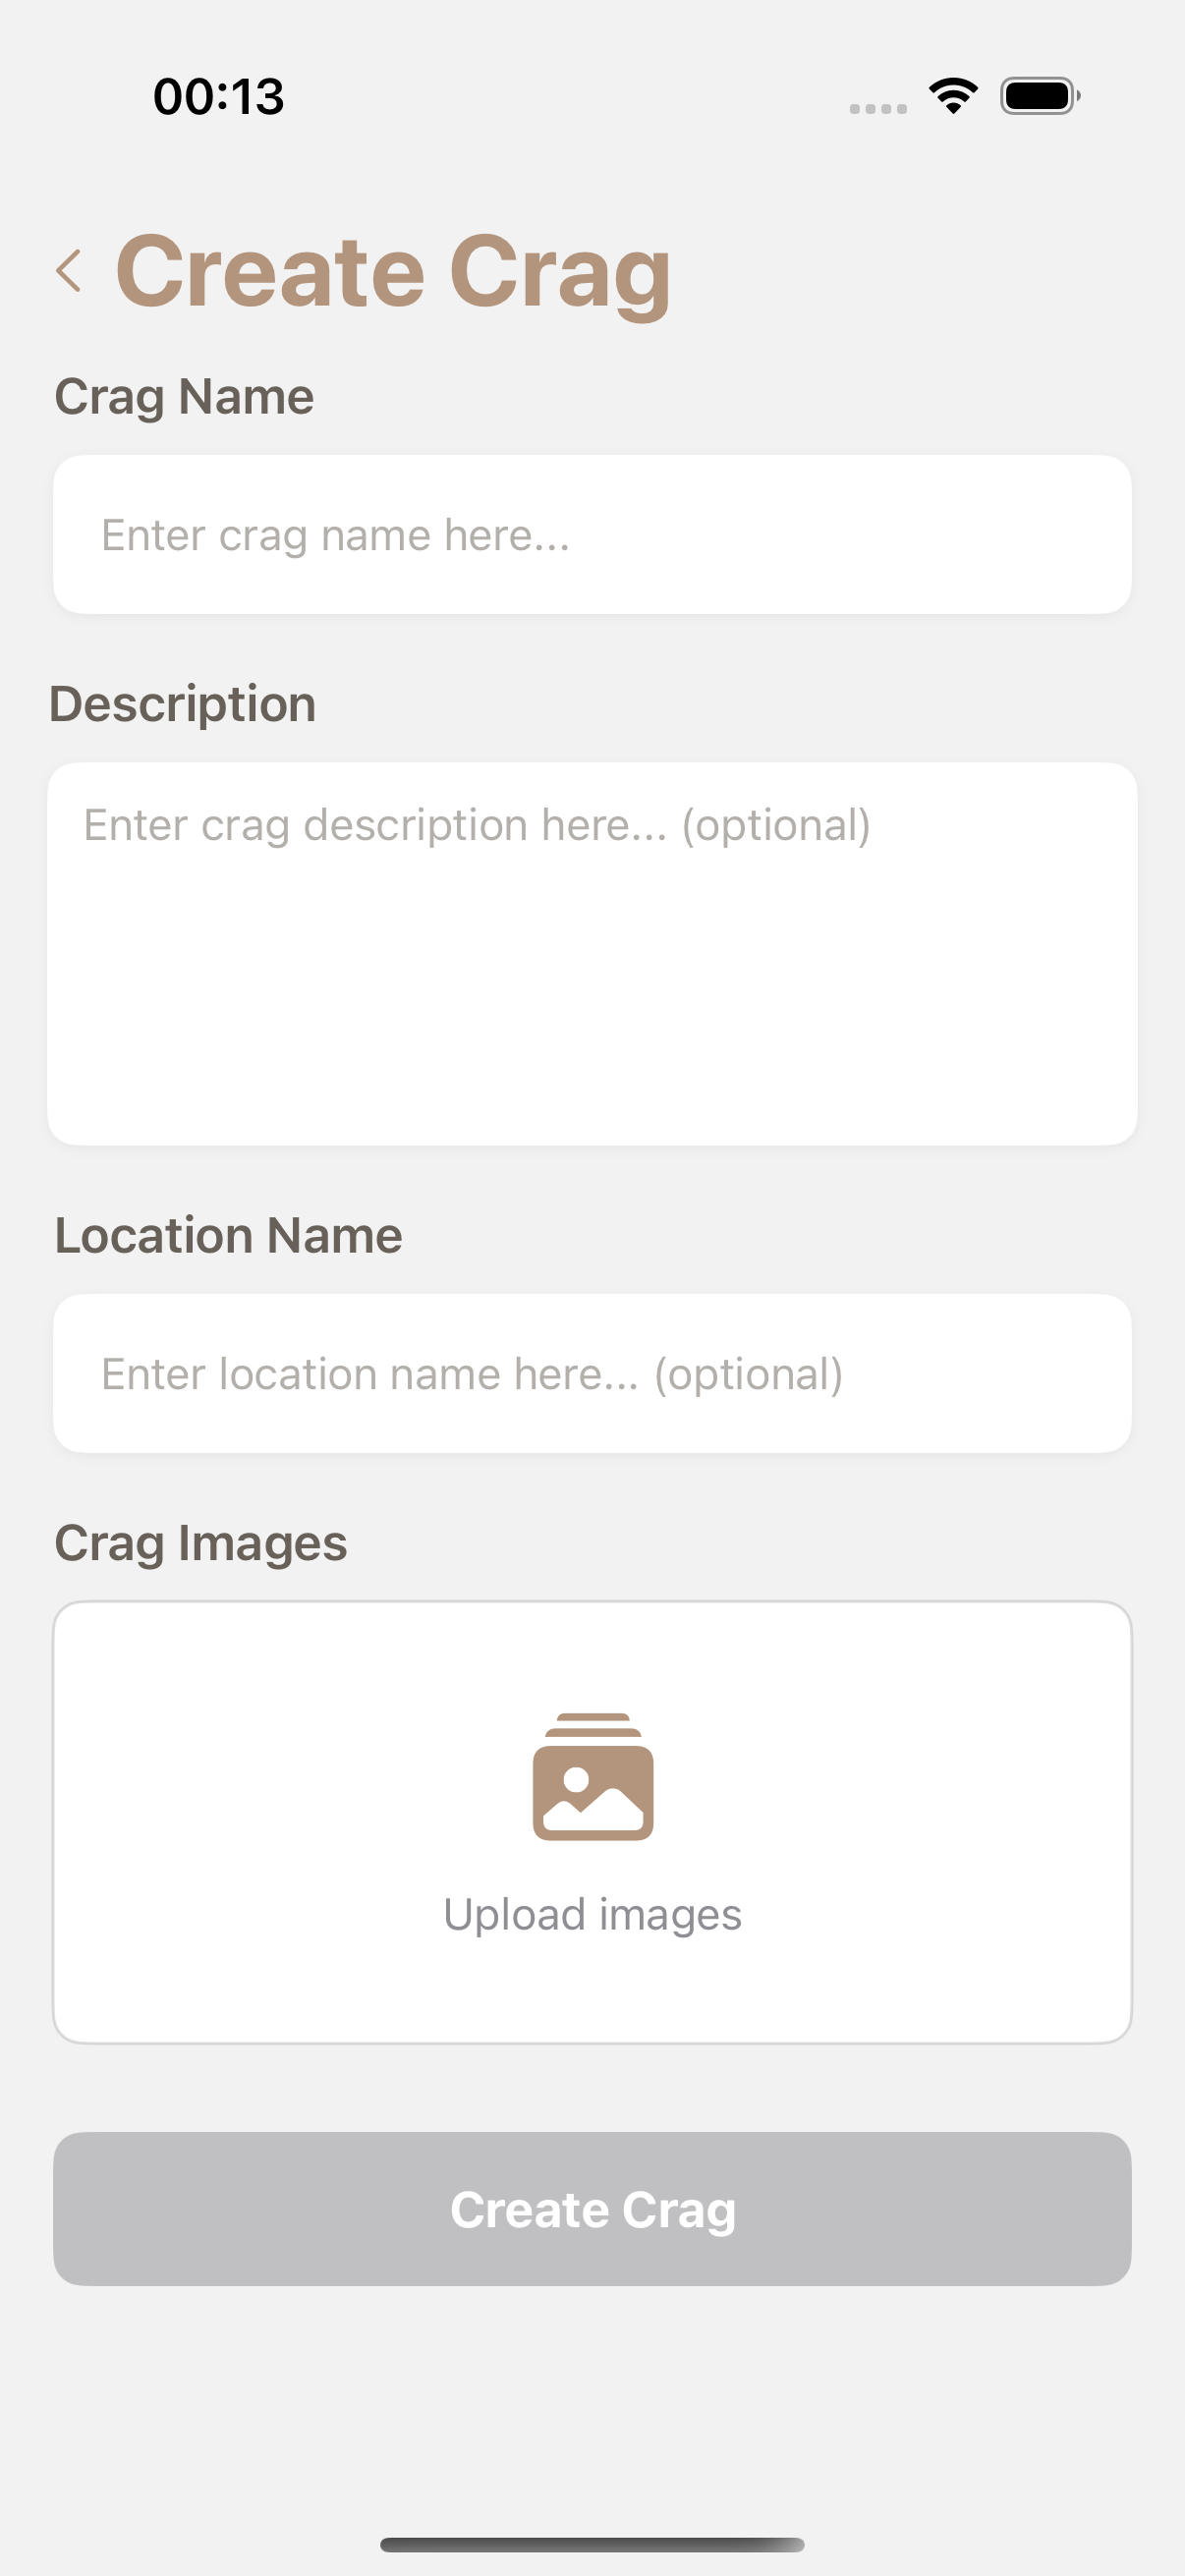
\includegraphics[width=\textwidth]{images/implementacija/editing-options/create_crag.png}
        \caption{Mobilna aplikacija}
        \label{fig:dodavanje_lokacije_mob}
    \end{subfigure}
    \hfill
    \begin{subfigure}[b]{0.6\textwidth}
        \centering
        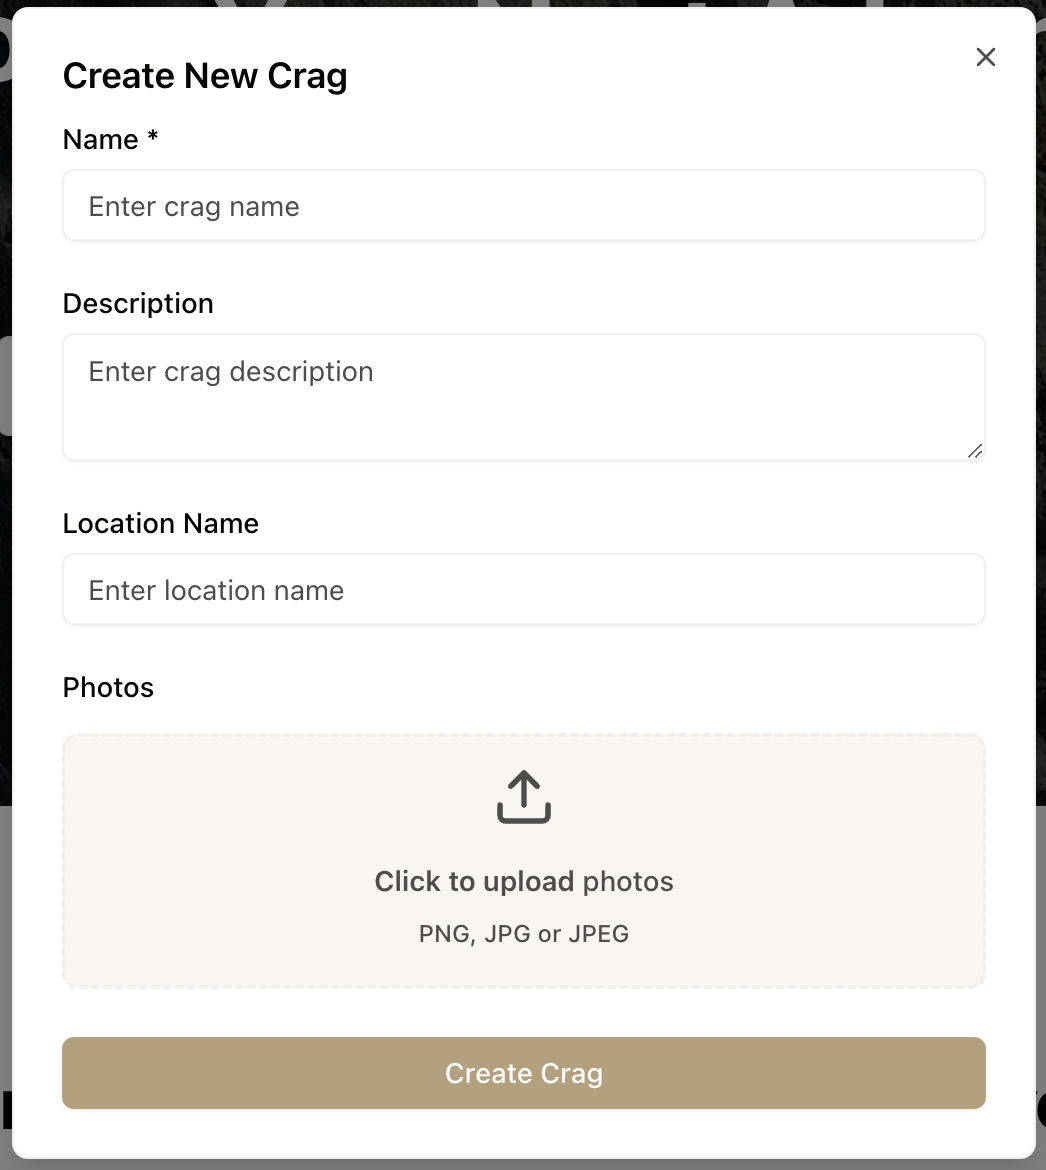
\includegraphics[width=\textwidth]{images/implementacija/web/editing-options/create-crag.png}
        \caption{Web aplikacija}
        \label{fig:dodavanje_lokacije_web}
    \end{subfigure}
    \caption{Dodavanje novog penjališta}
    \label{fig:dodavanje_lokacije}
\end{figure}

Ovlašteni korisnik odabirom ove opcije pristupa formi za unos novog (slika~\ref{fig:dodavanje_lokacije}). Potrebno je unijeti naziv penjališta, opcionalni opis koji može sadržavati informacije o povijesti regije ili slične zanimljivosti, te naziv šire geografske lokacije. Ime geografske lokacije korisnik može samostalno dodati, no ako ne postoji, aplikacija će automatski dodati naziv geografske lokacije na temelju lokacije penjališta. Ključno, korisnik može dodati jednu ili više fotografija koje vizualno predstavljaju penjalište. Nakon unosa svih podataka, novo penjalište se stvara u sustavu i postaje dostupna svim korisnicima.

\begin{figure}[H]
    \centering
    \begin{subfigure}[b]{0.36\textwidth}
        \centering
        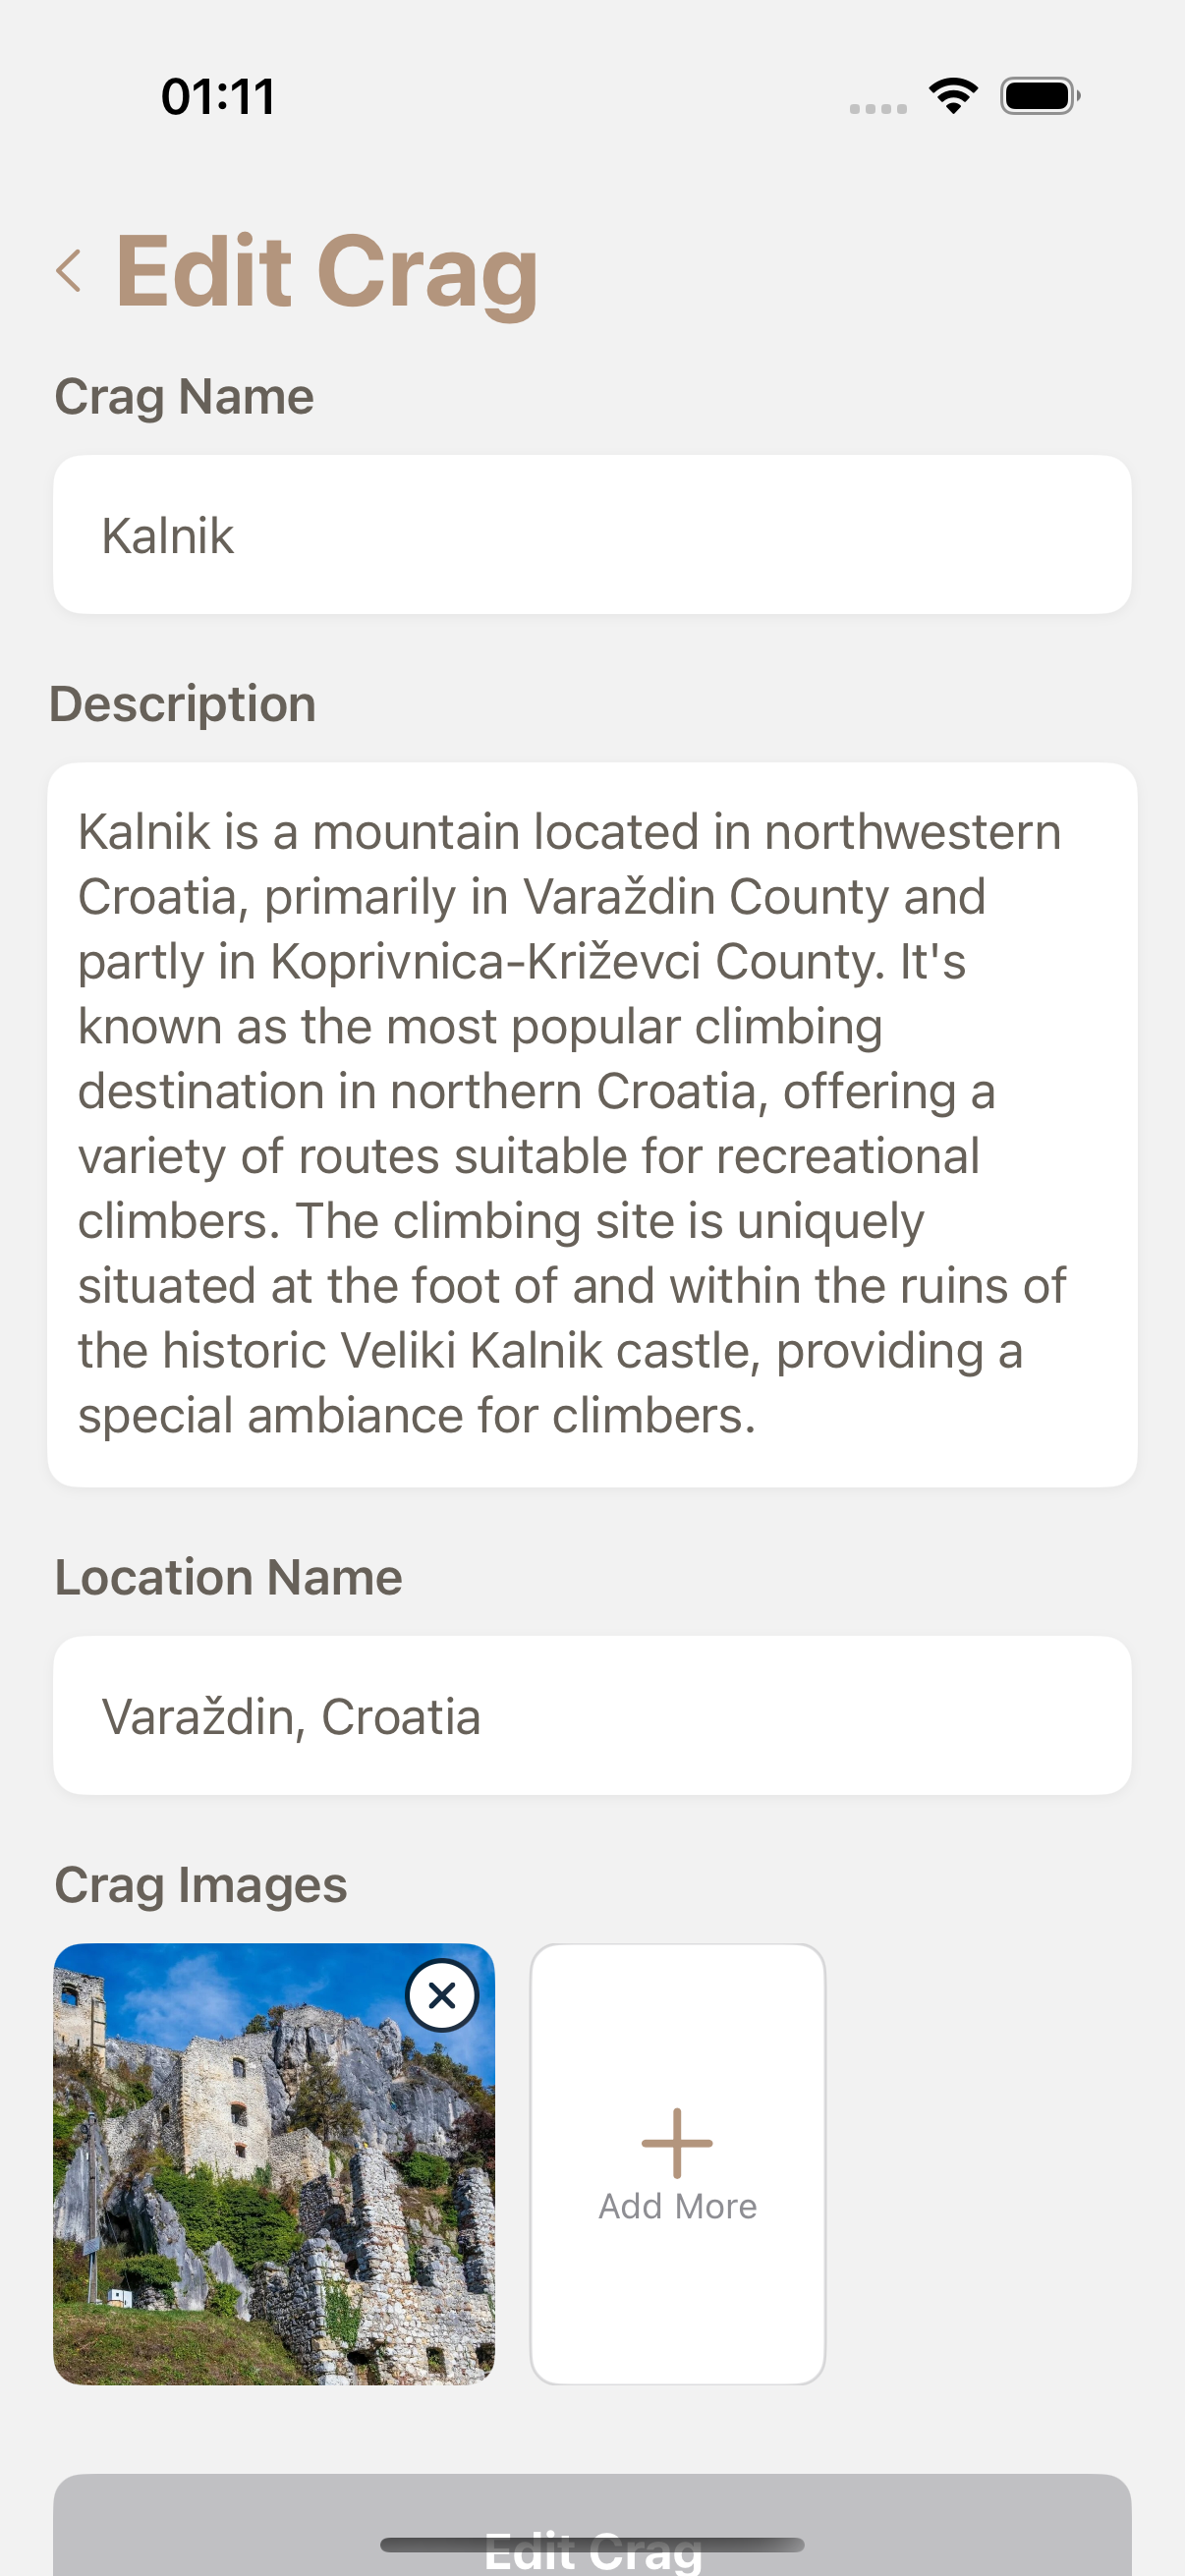
\includegraphics[width=\textwidth]{images/implementacija/editing-options/edit-crag.png}
        \caption{Mobilna aplikacija}
        \label{fig:uredjivanje_lokacije_mob}
    \end{subfigure}
    \hfill
    \begin{subfigure}[b]{0.47\textwidth}
        \centering
        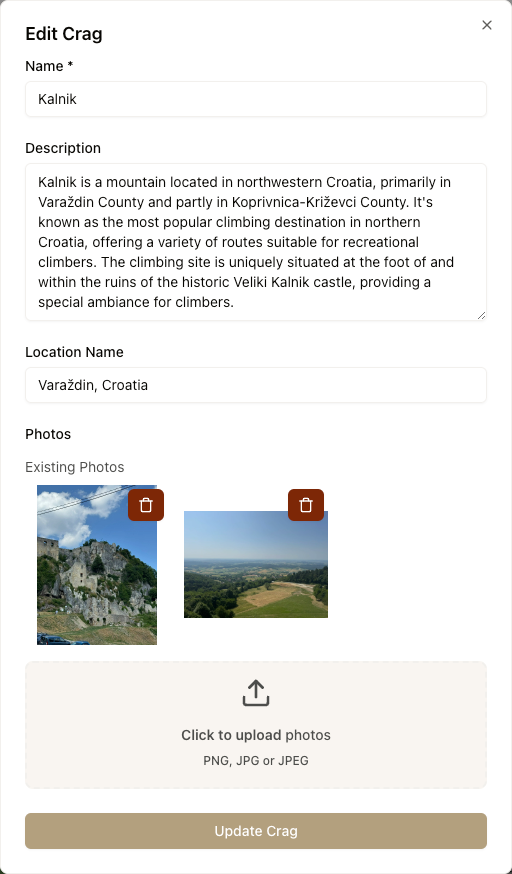
\includegraphics[width=\textwidth]{images/implementacija/web/editing-options/edit-crag.png}
        \caption{Web aplikacija}
        \label{fig:uredjivanje_lokacije_web}
    \end{subfigure}
    \caption{Uređivanje postojećeg penjališta}
    \label{fig:uredjivanje_lokacije}
\end{figure}

Osim kreiranja novih, ovlašteni korisnici imaju mogućnost i uređivanja postojećih penjališta (slika~\ref{fig:uredjivanje_lokacije}). Pristup ovoj funkcionalnosti omogućen je u izborniku na zaslonu s detaljnim pregledom penjališta. 
Sučelje za uređivanje omogućuje promjenu svih prethodno unesenih podataka, uključujući naziv, opis i naziv geografske lokacije. Korisnici također mogu upravljati galerijom fotografija, dodajući nove ili uklanjajući postojeće slike. 

Brisanje penjališta dostupno je u izborniku na zaslonu detaljnog pregleda penjališta. Klikom na opciju "Izbriši penjalište" (eng. \textit{Delete crag}) korisniku se prikazuje prozor s upitom o potvrdi brisanja. Ako korisnik potvrdi brisanje, penjalište se briše iz sustava i postaje nedostupno svim korisnicima.

\subsection{Upravljanje korisničkim ovlastima}

Kako bi se osigurala kontrola nad unosom i uređivanjem podataka, a istovremeno omogućio doprinos više ljudi, sustav implementira mehanizam za upravljanje korisničkim ovlastima na razini pojedine penjališta. Ovoj funkcionalnosti imaju pristup samo vlasnik penjališta i administratori sustava putem izbornika na zaslonu s detaljnim pregledom penjališta. 

\begin{figure}[H]
    \centering
    \begin{subfigure}[b]{0.36\textwidth}
        \centering
        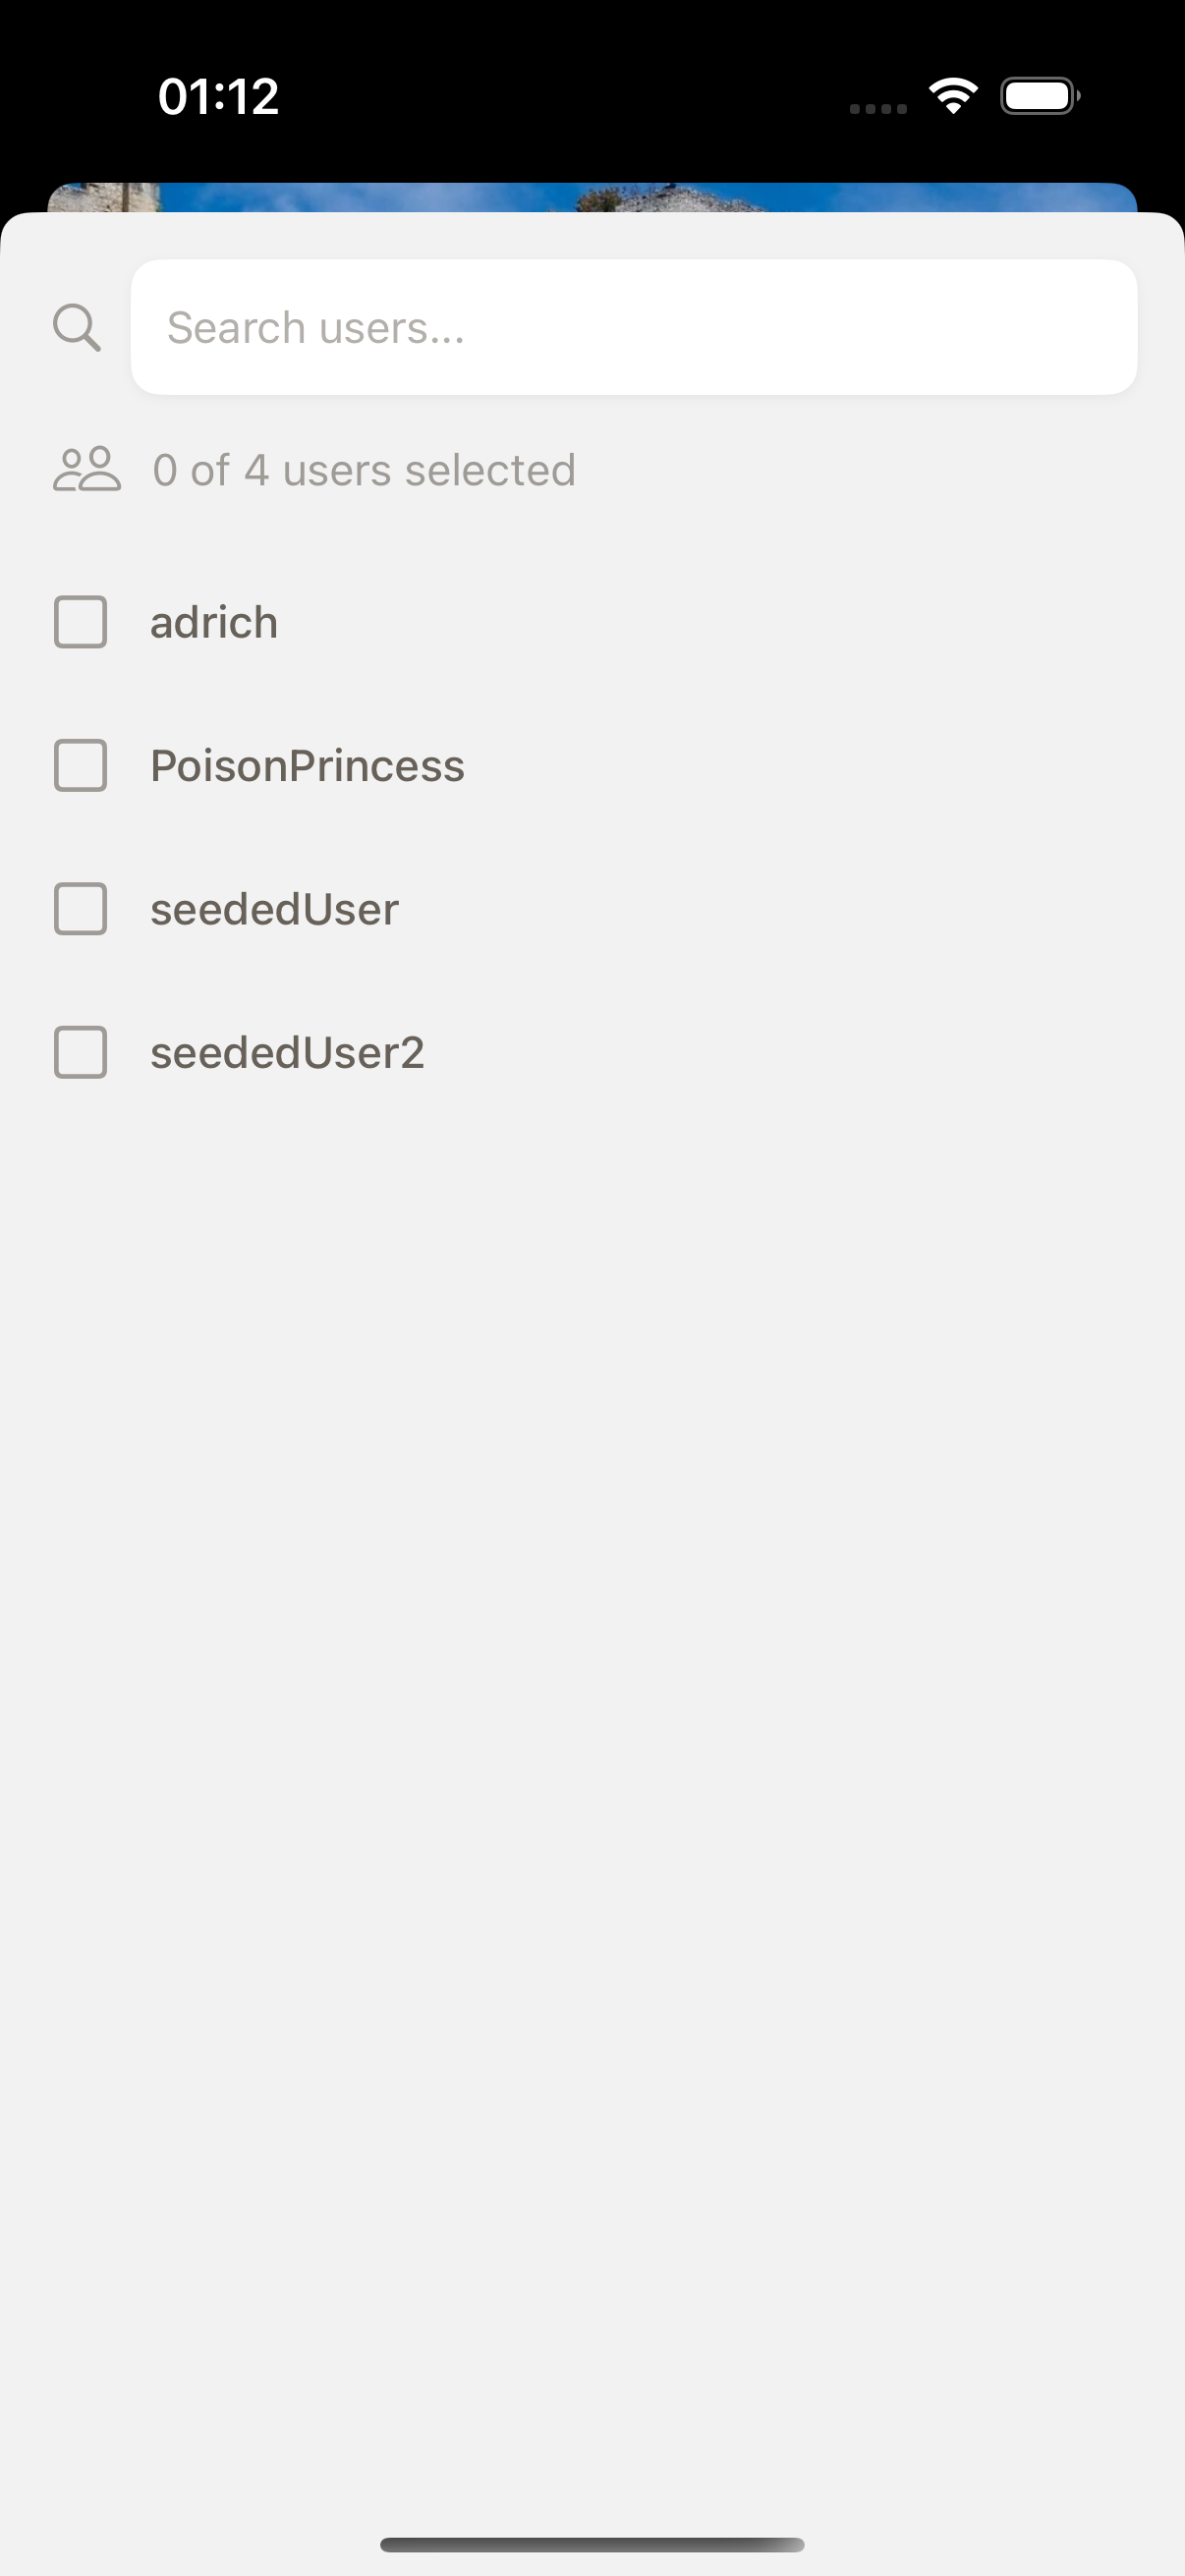
\includegraphics[width=\textwidth]{images/implementacija/editing-options/manage-users.png}
        \caption{Mobilna aplikacija}
        \label{fig:upravljanje_ovlastima_mob}
    \end{subfigure}
    \hfill
    \begin{subfigure}[b]{0.6\textwidth}
        \centering
        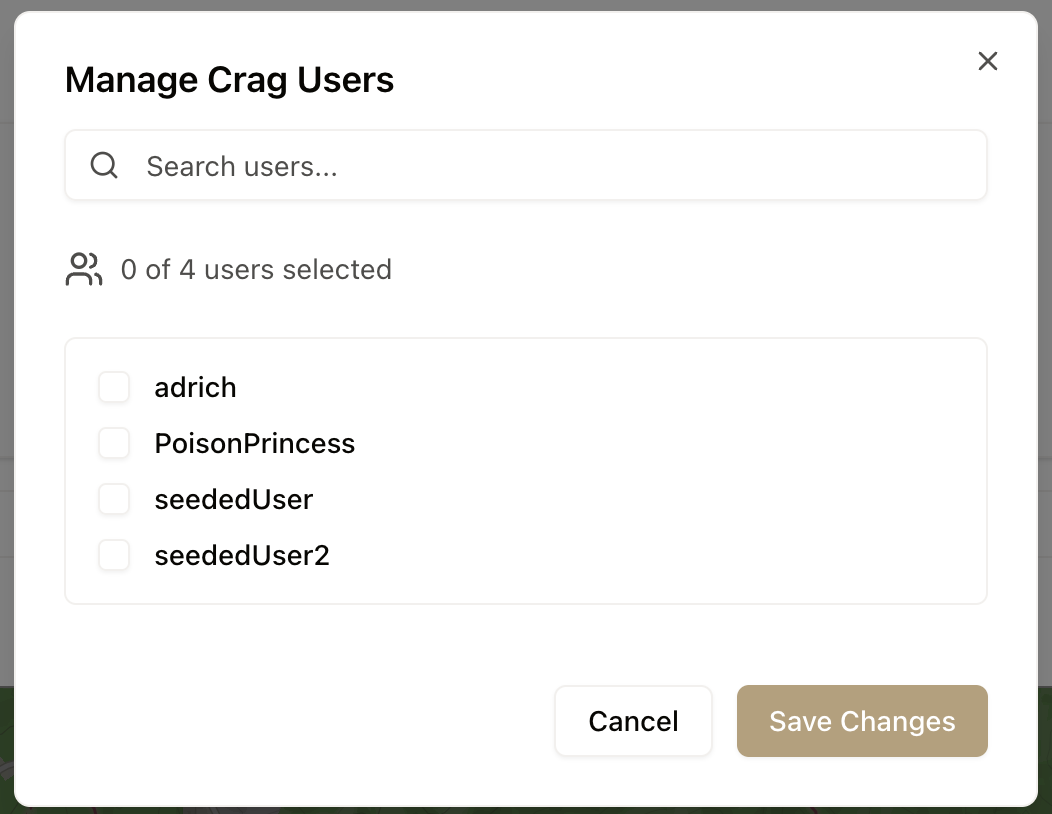
\includegraphics[width=\textwidth]{images/implementacija/web/editing-options/manage-users.png}
        \caption{Web aplikacija}
        \label{fig:upravljanje_ovlastima_web}
    \end{subfigure}
    \caption{Upravljanje korisničkim ovlastima}
    \label{fig:upravljanje_ovlastima}
\end{figure}

Pristupom pregledu za upravljanje ovlastima prikazuje se popis svih korisnika koji trenutno imaju ili mogu dobiti dozvole za uređivanje sadržaja na tom penjalištu (slika~\ref{fig:upravljanje_ovlastima}). Sučelje omogućuje pretragu korisnika po korisničkom imenu te odabir jednog ili više korisnika kojima se žele dodijeliti ili oduzeti ovlasti uređivanja. Time odabrani korisnik dobiva prava uređivanja penjališta bez davanja potpunih administrativnih ili kreator prava.


\subsection{Dodavanje, uređivanje i brisanje sektora}

Unutar svakog penjališta, ovlašteni korisnici mogu dalje strukturirati sadržaj kreiranjem i uređivanjem sektora. Pristup opciji za dodavanje nalazi se u izborniku na zaslonu s detaljnim pregledom penjališta. 

\begin{figure}[H]
    \centering
    \begin{subfigure}[b]{0.36\textwidth}
        \centering
        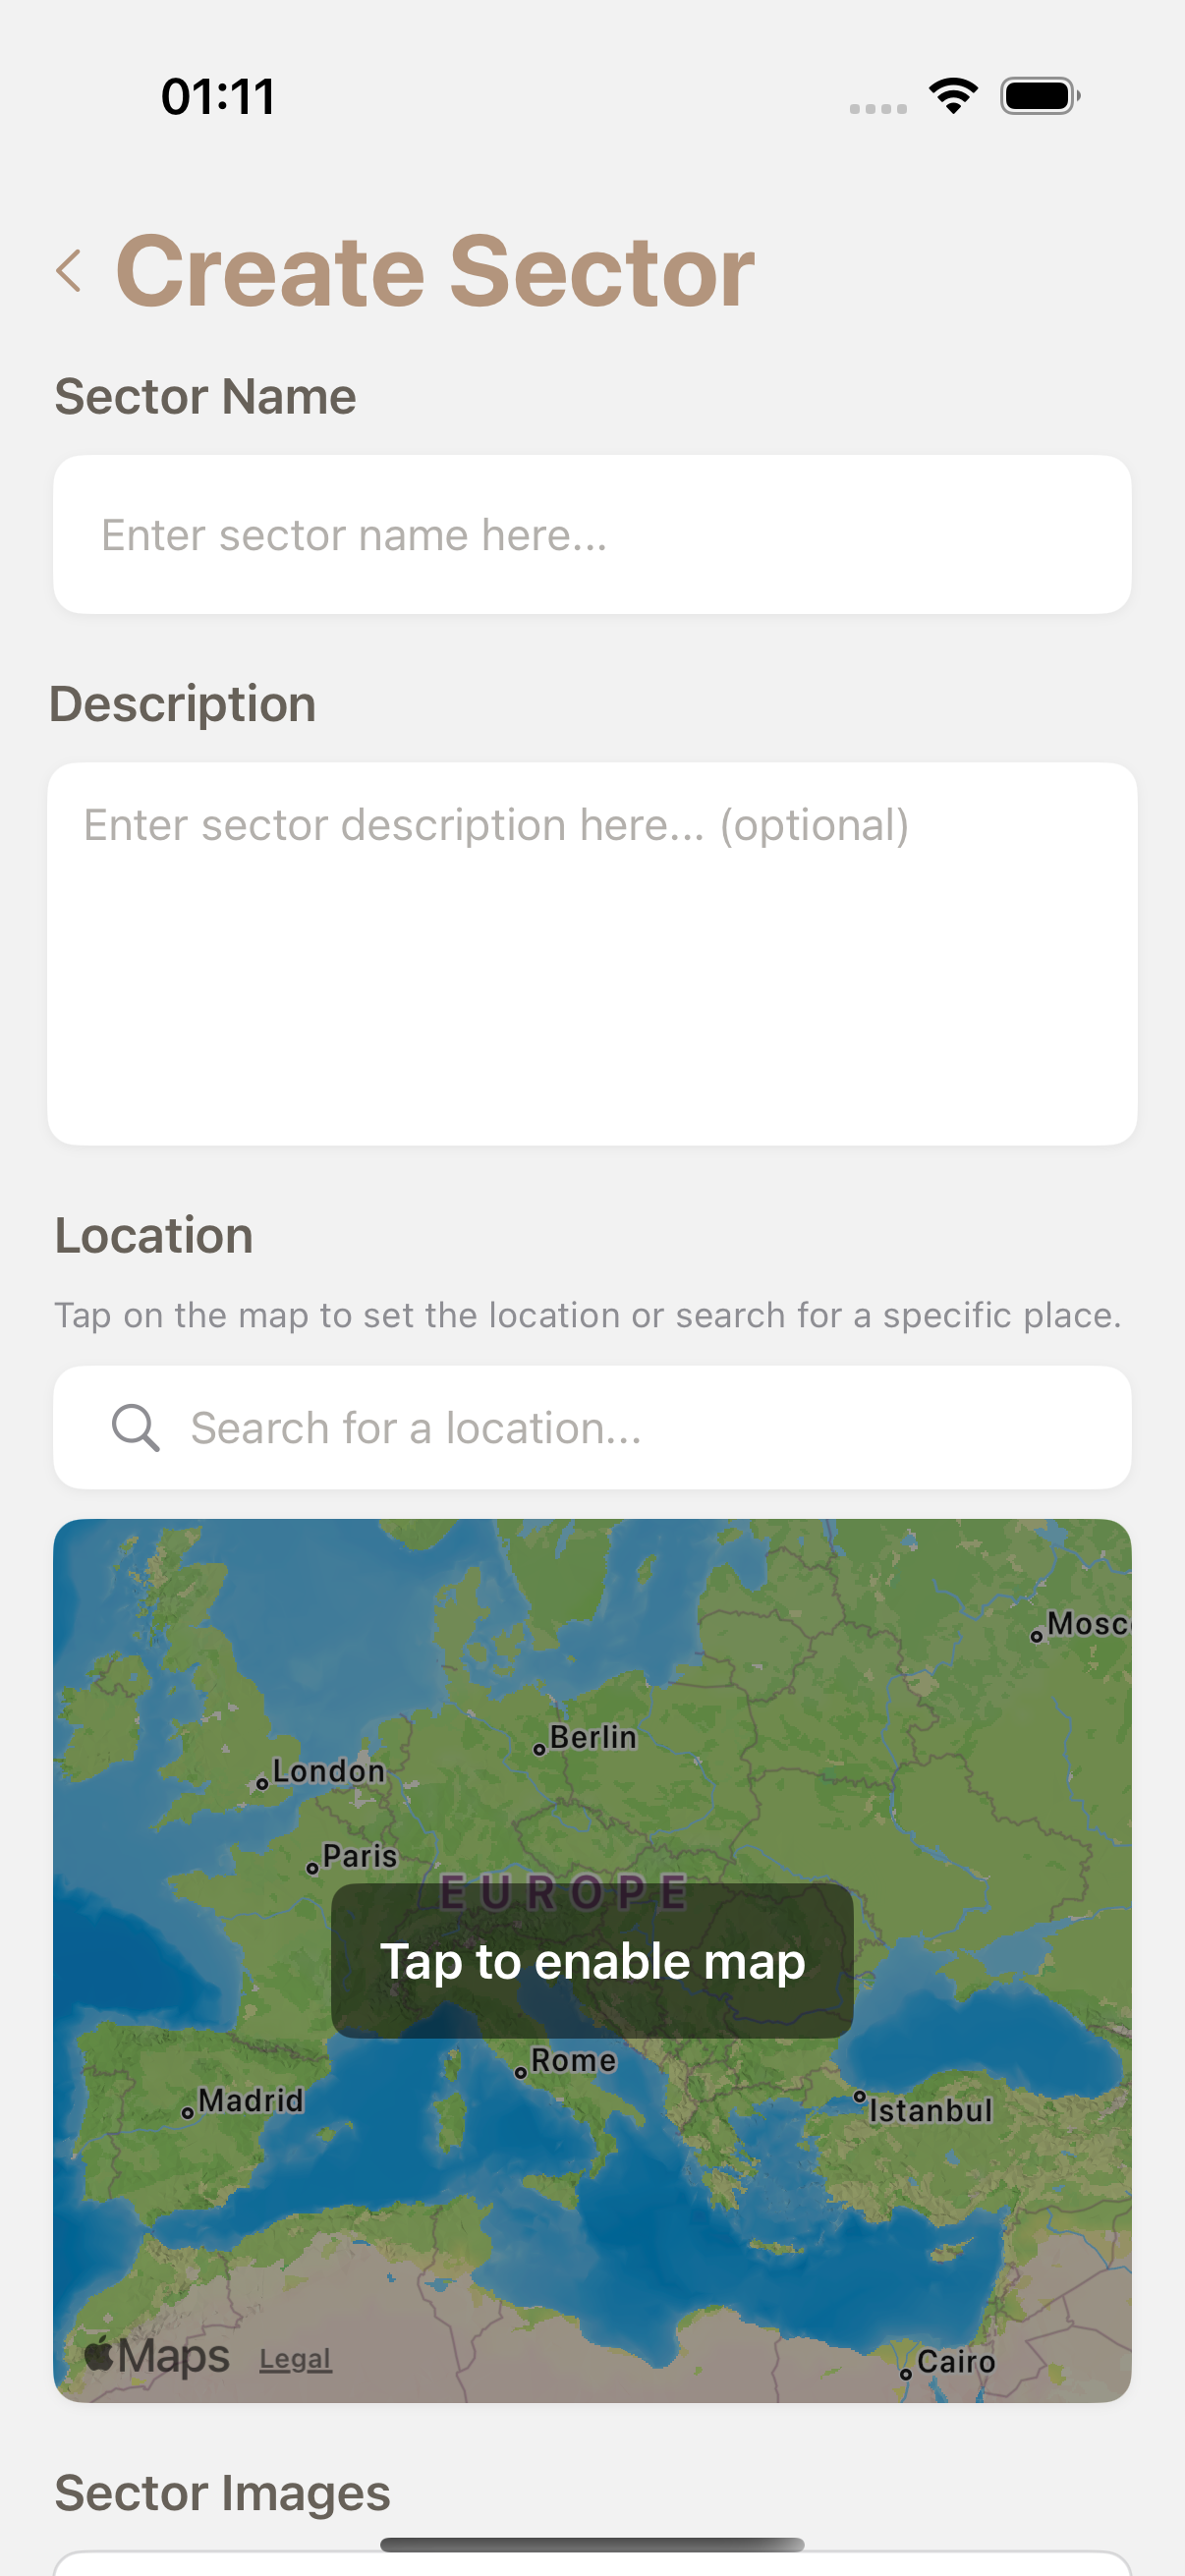
\includegraphics[width=\textwidth]{images/implementacija/editing-options/create-sector.png}
        \caption{Mobilna aplikacija}
        \label{fig:dodavanje_sektora_mob}
    \end{subfigure}
    \hfill
    \begin{subfigure}[b]{0.45\textwidth}
        \centering
        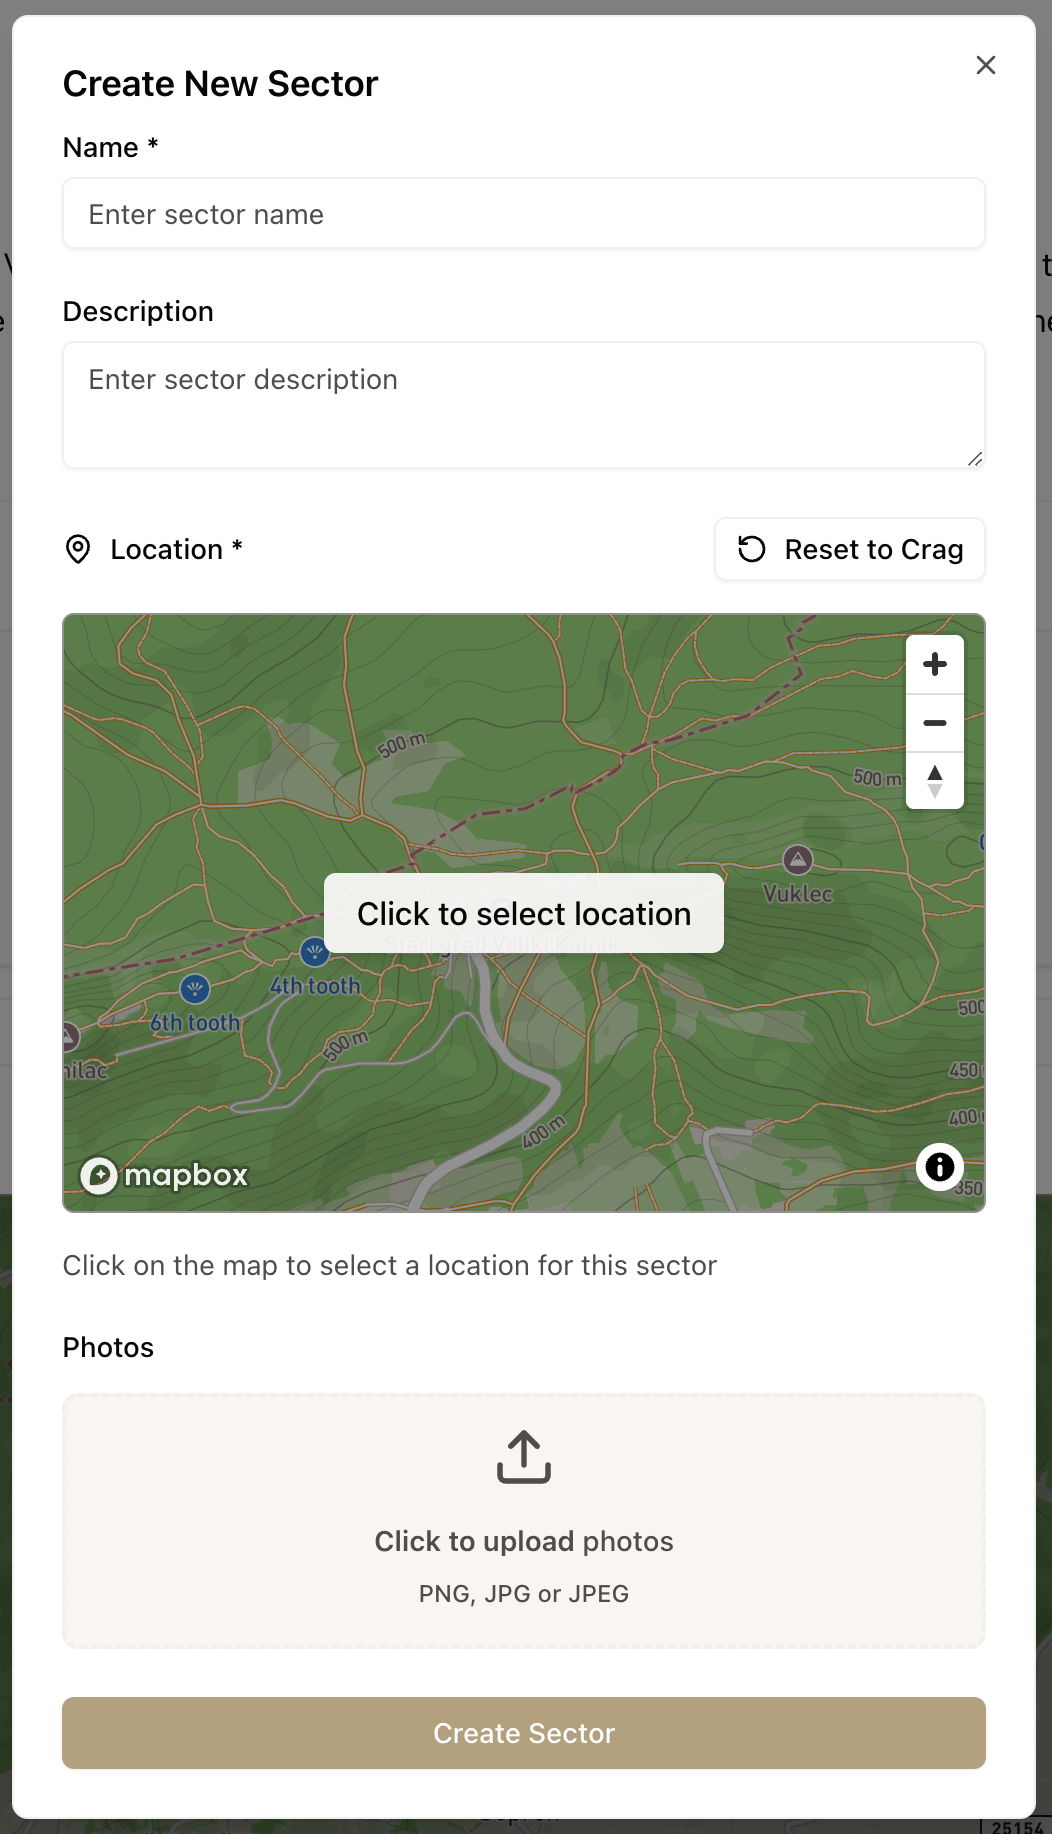
\includegraphics[width=\textwidth]{images/implementacija/web/editing-options/create-sector.png}
        \caption{Web aplikacija}
        \label{fig:dodavanje_sektora_web}
    \end{subfigure}
    \caption{Dodavanje novog sektora}
    \label{fig:dodavanje_sektora}
\end{figure}

Forma za unos novog sektora zahtijeva od korisnika unos naziva sektora i opcionalnog opisa, koji može sadržavati specifične informacije koje su specifične za sektore te ostale relevantne informacije (slika~\ref{fig:dodavanje_sektora}). Osim naziva zahtjeva se i upis lokacije u obliku koordinata. Pregledi taj proces olakšavaju uporabom geografske karte, koja omogućuje korisniku da odabere lokaciju sektora na karti ili pretraživanjem po nazivu lokacije. Kao i kod penjališta, moguće je dodati jednu ili više fotografija koje vizualno predstavljaju sektor.

Postojeći sektori mogu se uređivati na sličan način. Odabirom određenog sektora, korisniku se prikaže izbornik u kojem se nalazi opcija za uređivanje sektora. Forma omogućuje uređivanje  naziva, opisa, lokaciju i galeriju fotografija. (slika~\ref{fig:uredjivanje_sektora})

\begin{figure}[H]
    \centering
    \begin{subfigure}[b]{0.38\textwidth}
        \centering
        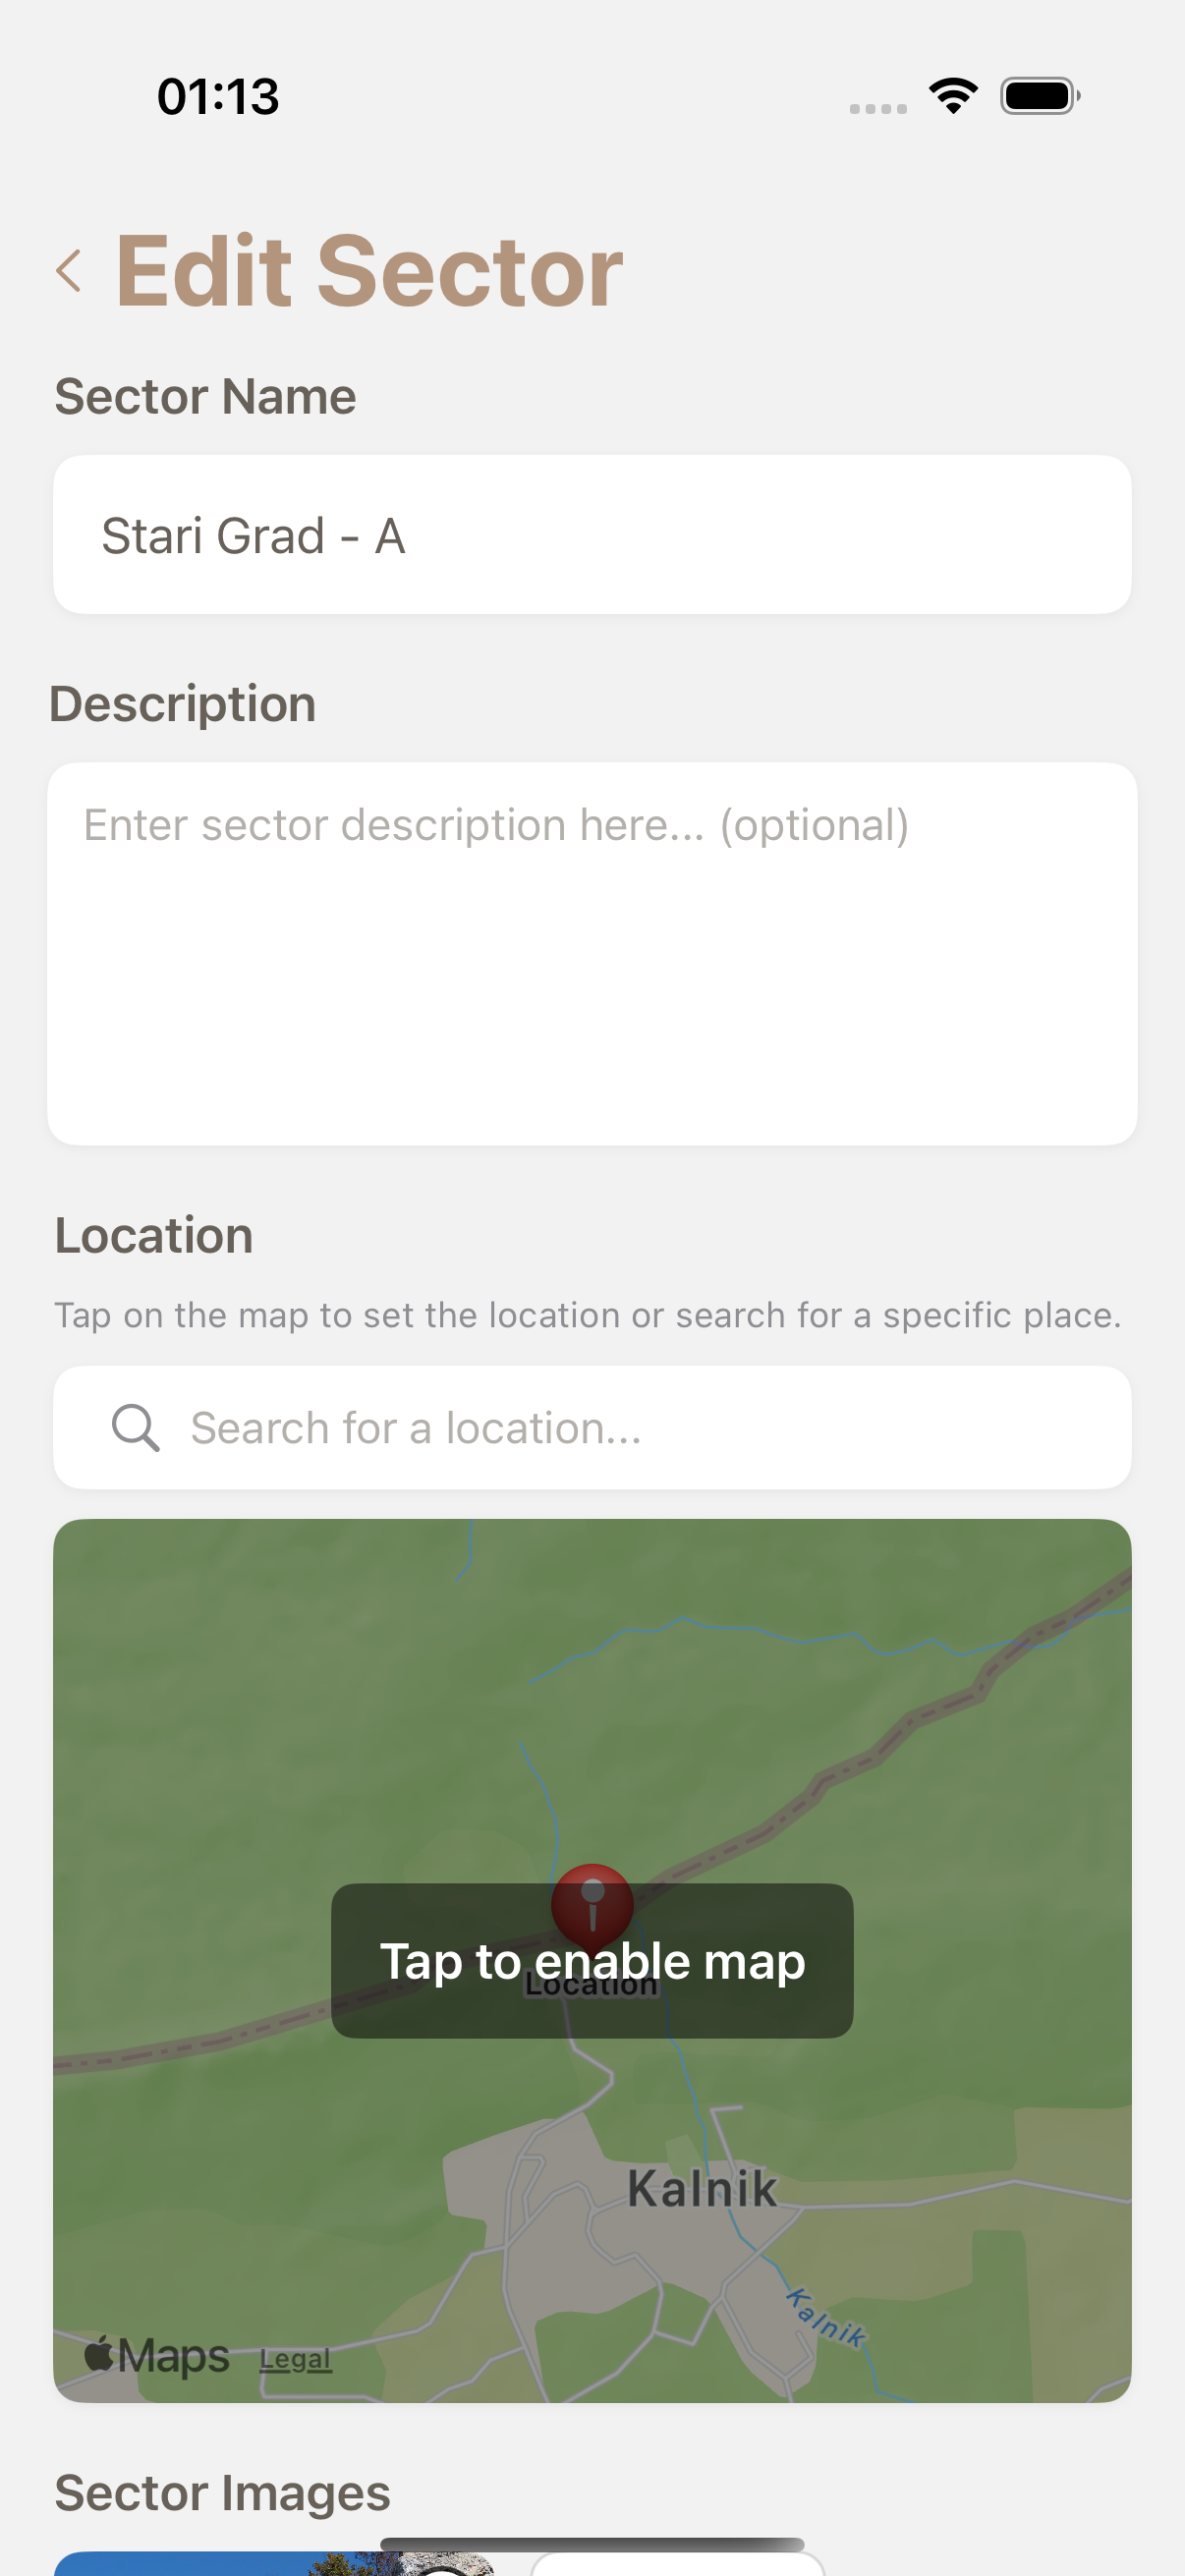
\includegraphics[width=\textwidth]{images/implementacija/editing-options/edit-sector.png}
        \caption{Mobilna aplikacija}
        \label{fig:uredjivanje_sektora_mob}
    \end{subfigure}
    \hfill
    \begin{subfigure}[b]{0.43\textwidth}
        \centering
        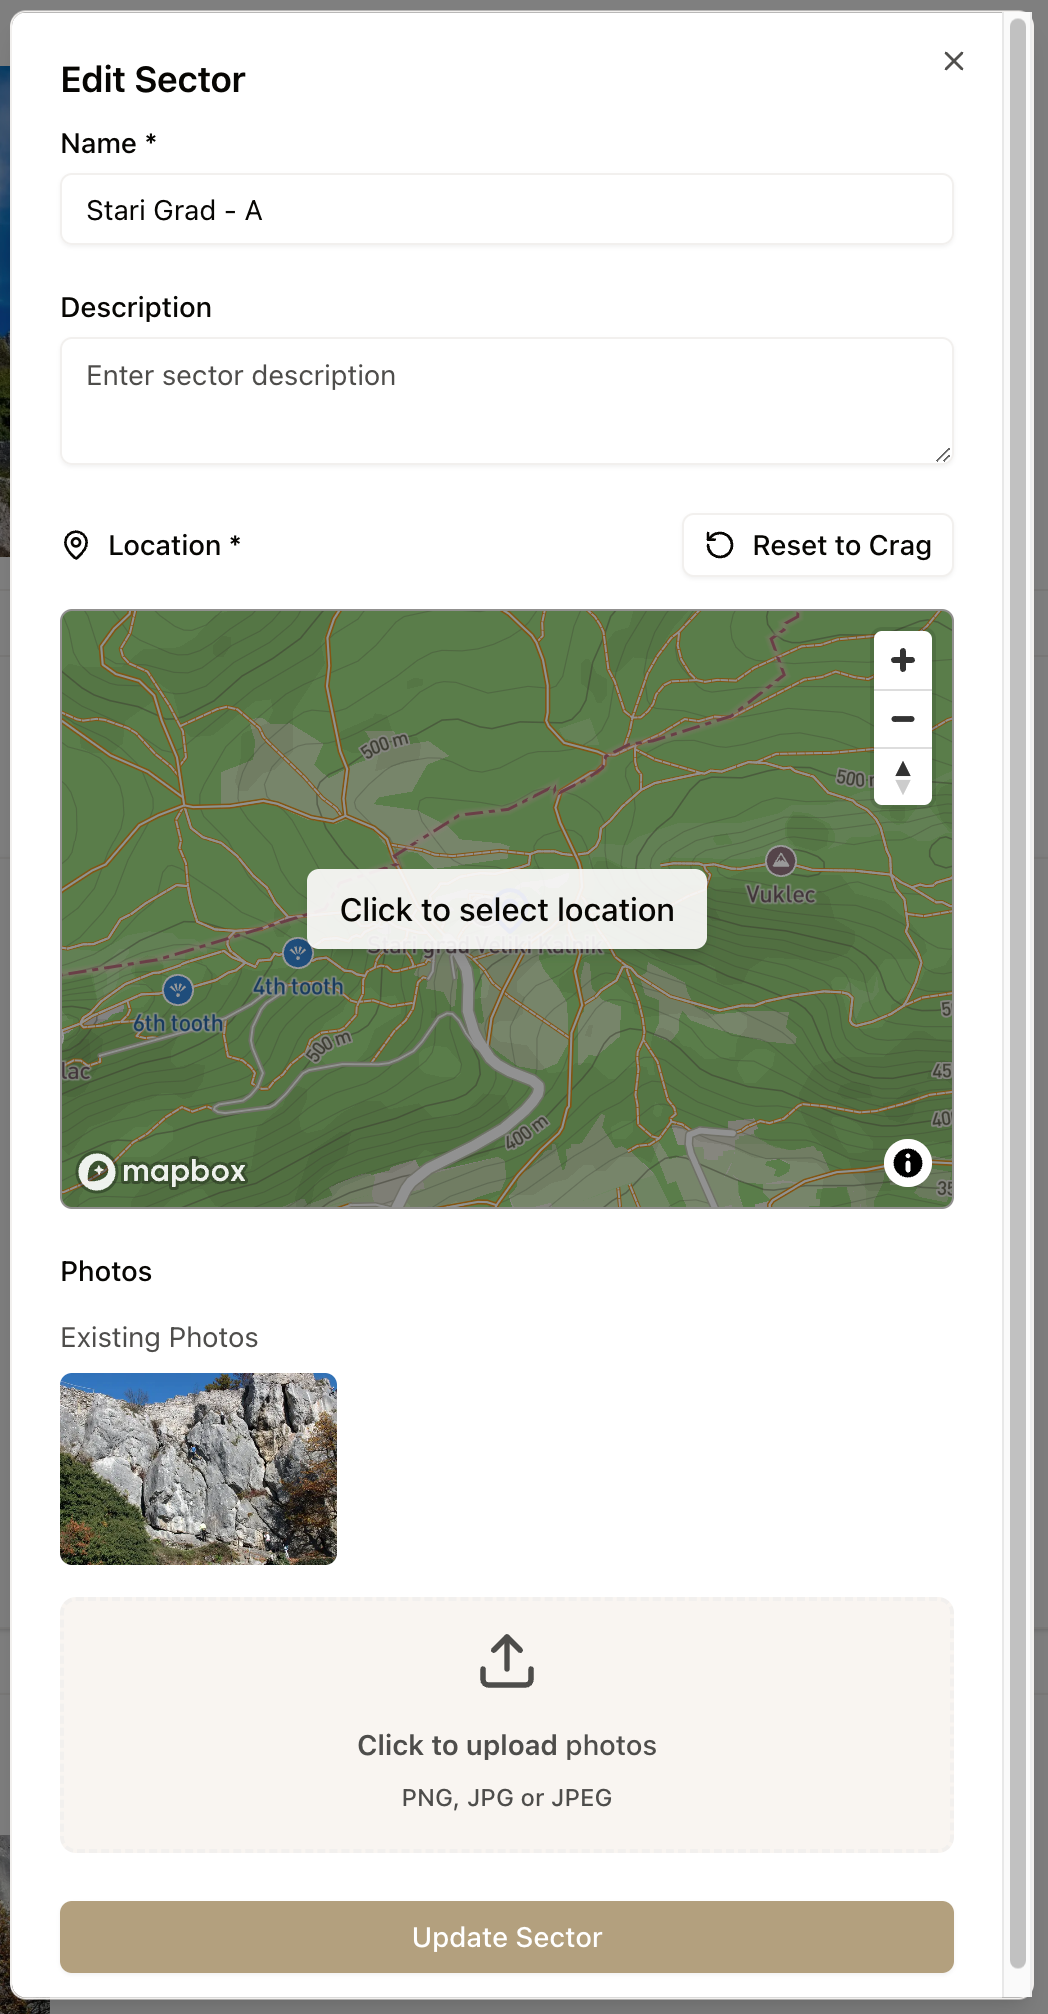
\includegraphics[width=\textwidth]{images/implementacija/web/editing-options/edit-sector.png}
        \caption{Web aplikacija}
        \label{fig:uredjivanje_sektora_web}
    \end{subfigure}
    \caption{Uređivanje postojećeg sektora}
    \label{fig:uredjivanje_sektora}
\end{figure}

Brisanje sektora dostupno je izborniku na zaslonu s detaljnim pregledom penjališta kada je označen penjački smjer. Klikom na opciju "Izbriši sektor" (eng. \textit{Delete sector}) korisniku se prikazuje prozor s upitom o potvrdi brisanja. Ako korisnik potvrdi brisanje, sektor se briše iz sustava i postaje nedostupno svim korisnicima.


\subsection{Dodavanje, uređivanje i brisanje penjačkih smjerova}

Na najnižoj hijerarhijskoj razini nalazi se unos i uređivanje pojedinačnih penjačkih smjerova. Ovlašteni korisnici mogu dodavati nove penjačke smjerove unutar određenog sektora. Pristup ovoj funkcionalnosti omogućen je u izborniku na zaslonu s detaljnim pregledom penjališta sa označenim sektorom. 

\begin{figure}[H]
    \centering
    \begin{subfigure}[b]{0.38\textwidth}
        \centering
        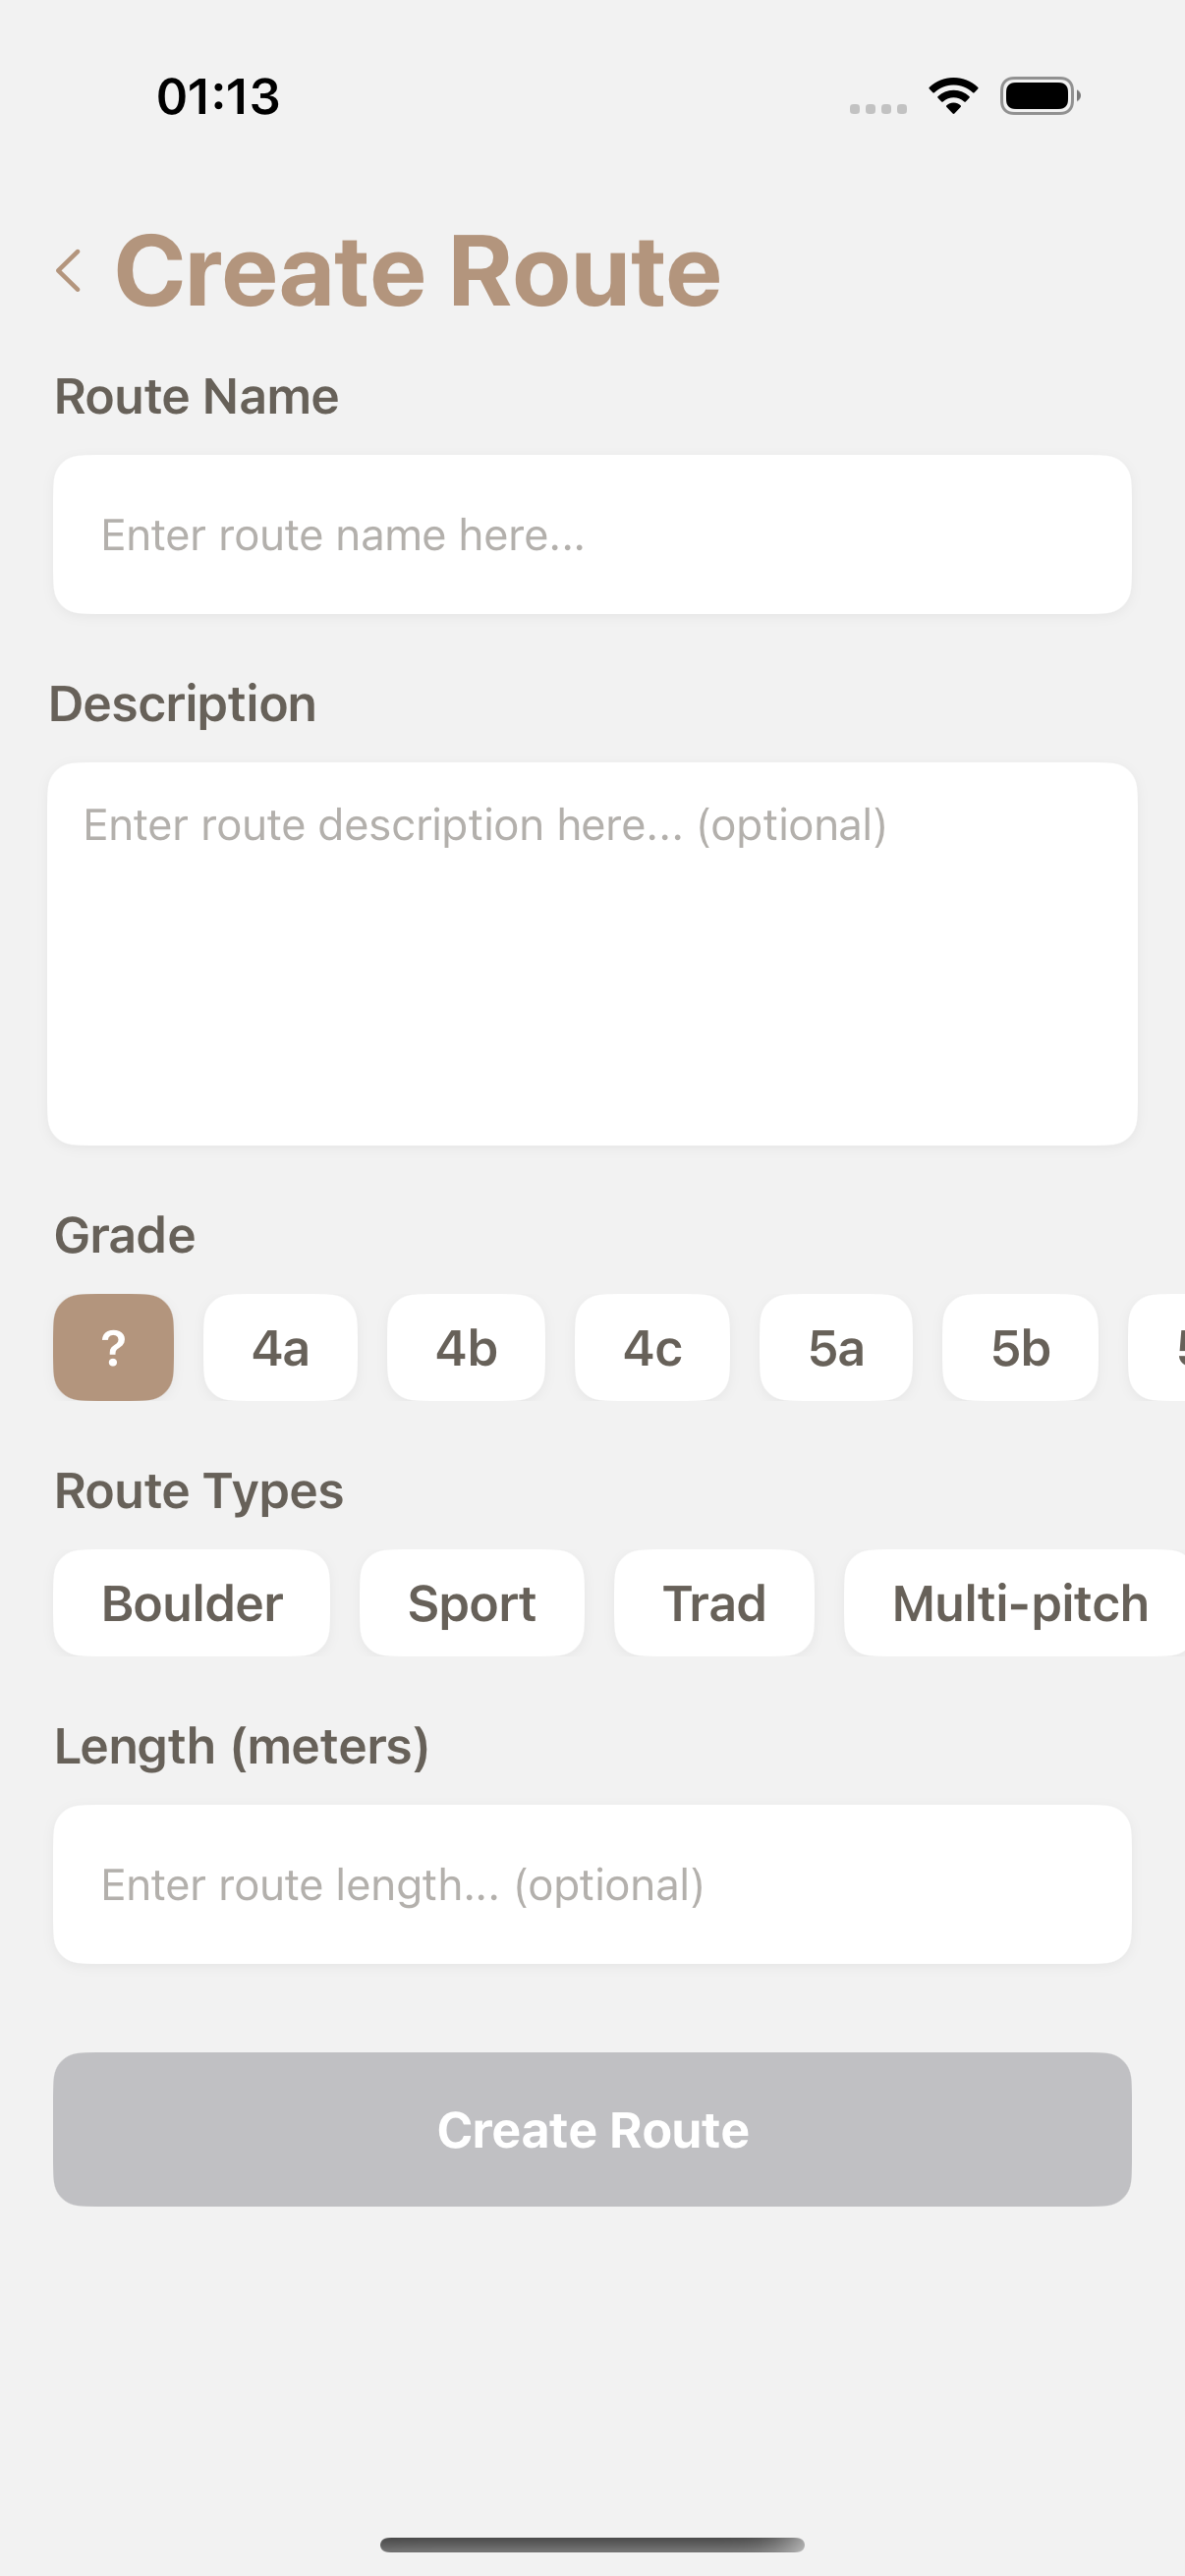
\includegraphics[width=\textwidth]{images/implementacija/editing-options/create-route.png}
        \caption{Mobilna aplikacija}
        \label{fig:dodavanje_smjera_mob}
    \end{subfigure}
    \hfill
    \begin{subfigure}[b]{0.55\textwidth}
        \centering
        \includegraphics[width=\textwidth]{images/implementacija/web/editing-options/create-route.png}
        \caption{Web aplikacija}
        \label{fig:dodavanje_smjera_web}
    \end{subfigure}
    \caption{Dodavanje novog penjačkog smjera}
    \label{fig:dodavanje_smjera}
\end{figure}

Forma za kreiranje novog penjačkog smjera uključuje polja poput naziva, opisa, težine, tipa penjačkog smjera i dužine (slika~\ref{fig:dodavanje_smjera}). Opcije za tip penjačkog smjera uključuju boulder, sportski, tradicionalni ili smjer s više penjačkih smjerova. 
Važno je primjetiti kako opcija dodavanja slike penjačkog smjera nije dostupna u formi za dodavanje novog penjačkog smjera. Dodavanje fotografije je moguće nakon kreiranja penjačkog smjera u pregledu detalja penjačkog smjera i dostupno je samo na mobilnoj aplikaciji. Klikom na izbornik u gornjem desnom kutu pregleda detalja penjačkog smjera, korisniku se prikazuje izbornik u kojem se nalazi opcija za dodavanje fotografije. Prvi korak u procesu dodavanja fotografije je slikanje penjačkog smjera pomoću kamere mobilnog uređaja. Nakon slikanja, korisniku se prikazuje slika na koju se može ručno ucrtati linija penjačkog smjera. Time je korisnik kreirao referentnu sliku penjačkog smjera koja se može koristiti za prepoznavanje penjačkog smjera (slika~\ref{fig:dodavanje_fotografije_smjera}).

\begin{figure}[H]
    \centering
    \includegraphics[width=0.3\textwidth]{images/implementacija/editing-options/add-route-photo.png}
    \caption{Dodavanje fotografije penjačkog smjera}
    \label{fig:dodavanje_fotografije_smjera}
\end{figure}

Uređivanje postojećeg penjačkog smjera dostupno je u izborniku na zaslonu s detaljnim pregledom tog penjačkog smjera. Na web aplikaciji izbornik se nalazi na izborniku u tablici kada je označen pregled svih sektora ili u listi kada je označen neki sektor. 

\begin{figure}[H]
    \centering
    \begin{subfigure}[b]{0.38\textwidth}
        \centering
        \includegraphics[width=\textwidth]{images/implementacija/editing-options/edit-route.png}
        \caption{Mobilna aplikacija}
        \label{fig:uredjivanje_smjera_mob}
    \end{subfigure}
    \hfill
    \begin{subfigure}[b]{0.55\textwidth}
        \centering
        \includegraphics[width=\textwidth]{images/implementacija/web/editing-options/edit-route.png}
        \caption{Web aplikacija}
        \label{fig:uredjivanje_smjera_web}
    \end{subfigure}
    \caption{Uređivanje postojećeg penjačkog smjera}
    \label{fig:uredjivanje_smjera}
\end{figure}

Forma omogućuje uređivanje svih podataka o penjačkom smjeru, uključujući naziv, opis, težinu, tip penjačkog smjera i dužinu, no također je omogućuje brisanje fotografija penjačkog smjera (slika~\ref{fig:uredjivanje_smjera}).


Brisanje penjačkog smjera dostupno je u izborniku na zaslonu s detaljnim pregledom penjačkog smjera. Klikom na opciju "Izbriši smjer" (eng. \textit{Delete route}) korisniku se prikazuje prozor s upitom o potvrdi brisanja. Ako korisnik potvrdi brisanje, penjački smjer se briše iz sustava i postaje nedostupno svim korisnicima.


\subsection{Uređivanje korisničkog profila}

Unutar korisničkog profila, u gornjem desnom kutu, nalazi se izbornik koji sadrži dodatne opcije za upravljanje računom i, ovisno o korisnikovim ovlastima, za doprinos sadržaju aplikacije. Odabirom opcije "Uredi profil" (eng. \textit{Edit profile}) korisnik odlazi na stranicu za uređivanje svojih podataka. Moguće je promijeniti ime, prezime, korisničko ime i datum rođenja. Aplikacija također omogućuje promjenu profilne fotografije te ažuriranje lozinke (slika~\ref{fig:uredjivanje_profila}).

\begin{figure}[H]
    \centering
    \begin{subfigure}[b]{0.35\textwidth}
        \centering
        \includegraphics[width=\textwidth]{images/implementacija/editing-options/edit_profile.png}
        \caption{Mobilna aplikacija}
        \label{fig:uredjivanje_profila_mob}
    \end{subfigure}
    \hfill
    \begin{subfigure}[b]{0.55\textwidth}
        \centering
        \includegraphics[width=\textwidth]{images/implementacija/web/editing-options/edit-user.png}
        \caption{Web aplikacija}
        \label{fig:uredjivanje_profila_web}
    \end{subfigure}
    \caption{Uređivanje korisničkog profila}
    \label{fig:uredjivanje_profila}
\end{figure}
% \section{Izvanmrežni način rada}

Penjališta se često nalaze na udaljenim lokacijama s ograničenim ili nepostojećim internetskim signalom. Zbog toga aplikacija implementira izvanmrežni način rada kako bi omogućila korisnicima korištenje aplikacije i situacijama slabog internetskog signala. Ova mogućnost je dostupna samo na mobilnoj aplikaciji. Korisnik može preuzeti podatke za bilo koje penjalište ili penjački smjer unutar detaljnog pregleda penjališta ili penjačkog smjera klikom na "Preuzmi penjalište" (eng. \textit{Download crag}) ili "Preuzmi penjački smjer" (eng. \textit{Download route}). Aplikacija tada pohranjuje sve podatke na lokalni uređaj, uključujući informacije o sektorima i penjačkim smjerovima, galerije forografija te najvažnije, referentne slike penjačkh smjerova potrebne za rad funkcionalnosti prepoznavanja penjačkih smjerova.

\begin{figure}[H]
    \centering
    \begin{subfigure}[b]{0.4\textwidth}
        \centering
        \includegraphics[width=0.7\textwidth]{images/implementacija/offline-mode/crag-tab.png}
        \caption{Popis preuzetih penjališta}
        \label{fig:offline_crag_tab}
    \end{subfigure}
    \hspace{0.08\textwidth}
    \begin{subfigure}[b]{0.4\textwidth}
        \centering
        \includegraphics[width=0.7\textwidth]{images/implementacija/offline-mode/routes-tab.png}
        \caption{Popis preuzetih penjačkih smjerova}
        \label{fig:offline_routes_tab}
    \end{subfigure}
    \caption{Izvanmrežni način rada - pregled preuzetih penjališta i smjerova}
    \label{fig:izvanmrezni_nacin_rada}
\end{figure}

Pristupom izvanmrežnom načinu rada, korisniku se prikazuje sučelje (slika~\ref{fig:izvanmrezni_nacin_rada}) s popisom svih penjališta i pojedinačnih penjačkih smjerova koje je prethodno preuzeo. Unutar ovog načina, korisnik može pregledavati sve preuzete podatke na gotovo identičan način kao i kada je spojen na internet. Detaljni pregled penjališta i smjerova zadržava sve ključne informacije i komponente, s iznimkom onih koje ovise o vanjskim servisima, poput vremenske prognoze i uređivanje podataka.
Najvažnije, funkcionalnost prepoznavanja penjačkih smjerova pomoću proširene stvarnosti je dostupna u izvanmrežnom načinu rada. Budući da su sve referentne slike pohranjene lokalno, proces detekcije i vizualizacije može se izvršavati neovisno o internetskoj vezi. Time se osigurava da ta funkcionalnost je dostupna penjačima upravo gdje je najpotrebnija - ispred same stijene.


% \chapter{Arhitektura i dizajn sustava "Alpinity"}

Kako bi se ostvarile prethodno opisane funkcionalnosti, sustav je koncipiran pomoću klijent-poslužitelj arhitekture. Ova arhitektura omogućuje fleksibilnost u razvoju aplikacije i direktno omogućuje korištenje različitih platformi za razvoj klijentskog softvera. Sustav se sastoji od tri neovisne komponente: centralnog pozadinskog sustava (eng. \textit{Backend}), mobilne aplikacije za iOS kao primarni klijent te web aplikacije kao komplementarnog klijenta. 
Komunikacija između klijenata i pozadinskog sustava odvija se putem definiranog REST servisa. Pozadinski sustav automatski generira OpenAPI specifikaciju koja služi kao formalna dokumentacija koju klijenti mogu koristiti za generiranje potrebnih funkcionalnosti za poziv servisa. Time se osigurava konzistentnost funkcionalnosti te olakšava paralelni razvoj.

\begin{figure}[H]
    \centering
    \includegraphics[width=0.9\textwidth]{images/arhitektura/general_arch.png}
    \caption{Makro arhitektura sustava}
    \label{fig:arhitektura}
\end{figure}

Slika~\ref{fig:arhitektura} prikazuje makro arhitekturu sustava te međusobne veze između komponenata. Mobilna i web aplikacija su neovisne komponente koje komuniciraju s pozadinskim sustavom putem REST servisa. Kada postoji neka slika, primjerice na detaljnom pregledu penjališta, pozadinski sustav šalje te slike u obliku poveznice na Azure Blog Storage servis. Također, web i mobilna aplikacije obije nemaju direktan pristup \textit{open-meteo} API-ju ni bazi podataka u obliku PostgreSQL baze podataka već se informacije agregiraju i šalju preko pozadinskog sustava.

\section{Pozadinski sustav (Backend)}

Pozadinski sustav predstavlja središnji dio cjelokupne arhitekture, odgovoran za svu poslovnu logiku, upravljanje podacima i komunikaciju s vanjskim servisima. Ključne odgovornosti pozadinskog sustava obuhvaćaju implementaciju RESTful API-ja za sve operacije, autentifikaciju i autorizaciju, te dohvaćanje i pohranu podataka iz relacijske baze podataka. Razvijen je korištenjem .NET platforme i ASP.NET core okvira, koji je odabran zbog visokih performansi i dobre podrške za razvoj modernih web servisa. Za organizaciju poslovne logike i smanjenje ovisnosti između unutarnjih komponenti pozadinskog sustava, sustav implementira Mediator uzorak (eng. \textit{Mediator pattern}). Ovaj pristup omogućuje da se zahtjevi s klijentskih aplikacija ponašaju kao neovisne poruke koje se zatim prosljeđuju odgovarajućim rukovateljima (eng. \textit{Handlers}), čime se postiže čišća arhitektura programskog koda. Pozadinski sustav podijeljen je u četri dijela.

\subsection{Sloj domene}

Sloj domene sadrži temeljnu poslovnu logiku i pravila koja su neovisna o bilo kojoj vanjskoj tehnologiji. Ovaj sloj nema ovisnosti o drugim slojevima u arhitekturi. Njegove ključne komponente su entiteti, koji predstavljaju objekte poslovne domene poput korisnika, penjališta, smjerova te objekte informacija vremenske prognoze i reverznog geokodiranja, definirajući njihovo stanje i ponašanje. Uz objekte domene, ovaj sloj sadrži i enumeracije koje predstavljaju moguće vrijednosti za određene objekte poput tipove penjačkih smjerova ili načine uspona.

\subsection{Aplikacijski sloj}

Aplikacijski sloj orkestrira korištenje domenskih objekata kako bi izvršio specifične korisničke slučajeve (eng. \textit {use cases}), djelujući kao posrednik između vanjskog svijeta i unutarnje poslovne logike. Za organizaciju, ovaj sloj implementira Mediator uzorak (engl. Mediator pattern). Svaki korisnički slučaj implementiran je kao trojka koji se sastoji od naredbe, što je poruka koja opisuje namjeru, validatora koji validira dobivenu naredbu te rukovatelja (engl. handler), klase koja prima poruku i izvršava potrebnu logiku. Ovaj sloj ovisi isključivo o sloju domene i definira logiku aplikacije bez znanja o tome kako će podaci biti prikazani ili pohranjeni.


\subsection{Infrastrukturni sloj}

Infrastrukturni sloj sadrži konkretne implementacije tehnologija koje su potrebne aplikaciji za rad. Ovaj sloj ovisi o aplikacijskom sloju kako bi implementirao njegova sučelja i sadrži sve što je promjenjivo i vanjsko. Ovdje se nalaze implementacije repozitorija koje koriste Entity Framework Core za komunikaciju s PostgreSQL bazom podataka. Također, ovaj sloj sadrži i integracije s vanjskim servisima: klijente za Azure Blob Storage za pohranu slika, open-meteo.com servis za vremensku prognozu i Mapbox servis za reverzno geokodiranje.

\subsection{Prezentacijski sloj}

Prezentacijski sloj je ulazna točka u pozadinski sustav, a u ovom slučaju to je ASP.NET Core Web API projekt. Njegova jedina odgovornost je primanje HTTP zahtjeva, prosljeđivanje odgovarajućih naredbi aplikacijskom sloju putem Mediator-a, te formatiranje rezultata u HTTP odgovore u JSON formatu. Ovaj sloj također automatski generira i OpenAPI specifikaciju, koja služi kao interaktivna dokumentacija API-ja i olakšava razvoj klijentskih aplikacija.


\subsection{Vanjski servisi}

Za pohranu slika, kao što su profilne slike korisnika i referentne slike penjačkih smjerova, koristi se Azure Blob Storage. Ovaj servis je odabran zbog pouzdanosti i lakoće integracije s pozadinskim sustavom. Kako bi se obogatile informacije penjališta koriste se dva vanjska servisa. Za dohvat detaljne vremenske prognoze penjališta koristi se open-meteo.com servis. Prednosti open-meteo servisa naspram drugih servisa za vremensku prognozu je mogućnost pregleda vremenske prognoze daleko u budućnosti, velike količine podataka koji se mogu dohvatiti te mogućnost izbora točno određenih podataka koji su potrebni. Za dohvat imena geografske lokacije iz GPS koordinata (reverzno geokodiranje) koristi se Mapbox servis. Mapbox servis je odabran jer je već korišten na web aplikaciji i nudi dobru podršku za reverzno geokodiranje.

\subsection{Model baze podataka}
Vidi sa mentoricom jel ovo previše.

\section{Mobilna aplikacija za iOS}

Mobilna aplikacija predstavlja primarni klijent sustava "Alpinity", posebice za korištenje na terenu. Razvijena je nativno za iOS platformu korištenjem SwiftUI okvira. SwiftUI je odabran kao moderno, deklarativno sučelje koje omogućuje razvoj kompleksnih korisničkih sučelja. Arhitektura aplikacije slijedi moderne principe razvoja za iOS, s jasnom podjelom odgovornosti između korisničkog sučelja, poslovne logike i komunikacije s pozadinskim sustavom. 

Za komunikaciju s pozadinskog sustava, aplikacija koristi swift-openapi-generator. Ovaj alat automatski generira Swift klijentski kod iz OpenAPI specifikacije, osiguravajući tipsku sigurnost i eliminirajući potrebu za ručnim pisanjem mrežnog sloja. Time se značajno ubrzava razvoj i smanjuje mogućnost pogrešaka. Za sigurno pohranjivanje korisničkog tokena za autentifikaciju i održavanje sesije, koristi se biblioteka KeychainAccess, koja pruža jednostavno i sigurno sučelje za rad s iOS Keychain servisom. Za prikaz interaktivnih geografskih karata, aplikacija se oslanja na nativni Apple Maps servis. Finalno, za spremanje podataka za izvanmrežni način rada, koristi se nativni SwiftData okvir.

\subsection{Implementacija prepoznavanja smjerova pomoću OpenCV}

Prepoznavanje penjačkih smjerova pomoću proširene stvarnosti implementirano je korištenjem biblioteke OpenCV. Svi računski intezivni zadaci računalnog vida izvršavaju se izravno na korisnikovom uređaju.

Da bi se postigao rad u stvarnom vremenu, ključno je efikasno upravljati kardovima koji dolaze s kamere. Aplikacija koristi moderni pristup temeljen na asinkronim tokovima podataka (eng. \textit{asynchronous streams}). Kamera kontinuirano emitira kadrove, no obrada svakog pojedinog kadra bila bi računski preskupa i dovela bi do zagušenja sustava. Zbog toga je implementiran mehanizam za prorjeđivanje kadrova (eng. \textit{frame dropping}). 
Koristi se \textit{AsyncStream} s politikom \textit{bufferingOldest(1)}, što znači da se u svakom trenutku čuva samo najstariji neobrađeni kadar. Ovaj pristup osigurava da sustav za obradu, time i korisnikov uređaj, nije preopterećen, čak i ako obrada jednog kadra traje duže od intervala između dva kadra.

Svaki kadar koji se propusti na obradu prolazi nizom operacija definiranih OpenCV funkcijama, sljedeći teorijske korake opisane u 3. poglavlju. Prvo se, radi optimizacije, smanjuje rezolucija ulaznog kadra ovisno o jačini prepoznavanja koje je korisnik postavio. Na tako pripremljenoj slici primjenjuje se SIFT algoritam pozivom metode \textit{sift.detectAndCompute}, koja ekstrahira ključne točke i njihove deskriptore. 
Nakon toga slijedi uparivanje s referentnim deskriptorima korištenjem \textit{flannMatcher.knnMatch} metode, a rezultati se filtriraju primjenom Loweovog testa omjera. Iz skupa preostalih dobrih podudarnosti, pozivom funkcije \textit{findHomography} s RANSAC metodom, izračunava se robusna matrica homografije.

Rezultat ovog procesa obrade je izobličena referentna slika linije penjačkog smjera s transparentnom pozadinom, dobivena primjenom izračunate homografije na originalnu sliku linije pomoću \textit{warpPerspective} funkcije. Ovakav izlaz omogućuje potpunu nezavisnost kadrova kamere i rezultata obrade kadrova, što omogućuje prikazivanje kadrova kamere bez ikakvih ograničenja, a rezultat se samo nadodaje na kadar kada se obradi. 
Ta slika ostaje spremljena i nacrtana preko novih kadrova dok se ne pojavi nova izobličena referentna slika. Ovakva organizacija procesa obrade omogućuje fluidno korisničko iskustvo sa nedostatkom što izobličene linije penjačkih smjerova kasne naspram kadrova. Unatoč ovom nedostatku, značajnija je prednost što jačina prepoznavanja može biti mnogo veća nego da se kadar kamere i izobličena referentna slika linije penjačkog smjera prikazuju sinkrono.

\subsection{Kreiranje referentne slike penjačkog smjera}

Aplikacija također sadrži i funkcionalnost za kreiranje referentnih podataka. Kada korisnik korištenjem kamere napravi sliku i na njoj iscrta putanju penjačkog smjera smjera, aplikacija poziva metodu koja prima niz koordinata koje predstavljaju putanju penjačkog smjera i referentnu sliku. Prvo stvara praznu, prozirnu matricu istih dimenzija kao i referentna slika. Dimenzija referentnih slika moraju biti identične kako bi algoritam mogao zamjeniti sliku s linijom prilikom procesa transformacije perspektive. Zatim, koristeći \textit{OpenCV} metodu \textit{polylines}, iscrtava liniju na tu matricu. Zanimljivo je da se linija iscrtava dva puta, prvo deblja crna linija, a zatim preko nje tanja crvena linija, čime se postiže vizualni efekt obruba. Rezultirajuća matrica se pretvara u sliku s linijom te se zatim šalje na poslužitelj i sprema na Azure Blob Storage i u bazu podataka kao poveznicu na Azure Blob Storage.


\section{Web aplikacija}

Uz mobilnu aplikaciju, sustav "Alpinity" uključuje i web aplikaciju. Njena temeljna svrha je pružiti korisnicima sučelje za pregled i upravljanje podacima na većim ekranima ili na android uređajima. Web aplikacija nudi sve funkcionalnosti dostupne na mobilnoj aplikaciji, s iznimkom onih koje su vezane uz hardver mobilnog uređaja, poput prepoznavanja smjerova pomoću kamere.

Aplikacija je razvijena korištenjem Next.js okvira, koji se temelji na React biblioteci. Next.js je odabran zbog svojih naprednih mogućnosti koje osiguravaju visoke performanse. Korištenjem tehnika poput renderiranja na poslužitelju postiže se iznimno brzo učitavanje sadržaja.

Korisničko sučelje je izgrađeno korištenjem biblioteke komponenata shadcn/ui. Ona omogućuje brzu i konzistentnu izradu vizualno dopadljivog i pristupačnog sučelja, temeljenog na prilagodljivim i višekratno iskoristivim komponentama. Za prikaz interaktivnih geografskih karata, web aplikacija koristi Mapbox platformu.

Komunikacija s pozadinskim sustavom riješena je na konzistentan i tipski siguran način. Korištenjem alata hey-api/openapi-ts, klijentski kod za pozivanje pozadinskog sustava automatski se generira iz OpenAPI specifikacije koju generira sam pozadinski sustav. Ovaj pristup, analogan onome korištenom u mobilnoj aplikaciji, osigurava da su klijent i poslužitelj uvijek usklađeni, smanjuje mogućnost pogrešaka i značajno ubrzava proces razvoja.
% \chapter{Testiranje i vrednovanje rješenja}

Nakon implementacije aplikacije, potrebno je provesti testiranje u realnim uvjetima kako bi se validirala funkcionalnost te procijenile performanse i praktična upotreba. Cilj poglavlja je analizirati rezultate testiranja, s posebnim naglaskom na funkcionalnost prepoznavanja penjačkih smjerova, te identificirati ograničenja i područja za poboljšanje.

\section{Metodologija testiranja}

Testiranje je provedeno na penjalištu Kalnik, koje zbog svoje popularnosti i raznolikosti stijena predstavlja prikladnu lokaciju za ispitivanje sustava. Za detaljnu analizu odabrana su dva penjačka smjera s različitim vizualnim karakteristikama kako bi se ispitala robusnost algoritma. 

\begin{figure}[H]
    \centering
    \begin{subfigure}[b]{0.45\textwidth}
        \centering
        \includegraphics[width=\textwidth]{images/testiranje/apaches_ref_slika.png}
        \caption{Referentna slika smjera "Apaches"}
        \label{fig:apaches}
    \end{subfigure}
    \hfill
    \begin{subfigure}[b]{0.45\textwidth}
        \centering
        \includegraphics[width=\textwidth]{images/testiranje/steyr_ref.png}
        \caption{Referentna slika smjera "Steyr"}
        \label{fig:steyr}
    \end{subfigure}
    \caption{Referentne slike odabranih penjačkih smjerova na penjalištu Kalnik}
    \label{fig:referentne_slike}
\end{figure}

Prvi primjer penjačkog smjera je "Apaches" u sektoru Stari Grad B (Slika~\ref{fig:apaches}). Smjer je lako prepoznatljiv zbog mnogo distinktnih značajki poput rupa, pukotina i varijacija u boji. Drugi primjer je smjer "Steyr" u sektoru Stari Grad A (Slika~\ref{fig:steyr}). Za razliku od "Apaches", smjer se nalazi na relativno glatkoj i uniformnoj stijeni s manje izraženih značajki, što predstavlja izazov za algoritam.

Za oba smjera prethodno su, putem aplikacije, kreirane referentne slike s ucrtanim linijama. Testiranje je izvršeno na uređaju iPhone 15 Pro u automatskom načinu rada primarno na "High" razini prepoznavanja, no također su testirane i niže razine "Medium" i "Low".


\section{Rezultati i analiza funkcionalnosti}

Sustav je u praksi potvrdio svoju funkcionalnost. Na smjeru "Apaches", koji je bogat značajkama, aplikacija brzo i stabilno prepoznaje stijenu te precizno projicira virtualnu liniju smjera preko video prikaza čak i iz različitih kutova (Slika~\ref{fig:apaches_test_double}) i korištenjem nižih razina prepoznavanja.

\begin{figure}[H]
    \centering
    \begin{subfigure}[b]{0.45\textwidth}
        \centering
        \includegraphics[width=\textwidth]{images/testiranje/apaches_test_left_side.png}
        \caption{Testiranje smjera "Apaches" s lijeve strane}
        \label{fig:apaches_test_left_side}
    \end{subfigure}
    \hfill
    \begin{subfigure}[b]{0.45\textwidth}
        \centering
        \includegraphics[width=\textwidth]{images/testiranje/apaches_test_right_side.jpeg}
        \caption{Testiranje smjera "Apaches" s desne strane}
        \label{fig:apaches_test_right_side}
    \end{subfigure}
    \caption{Testiranje smjera "Apaches" iz dva različita kuta}
    \label{fig:apaches_test_double}
\end{figure}

Testiranje je na zahtjevnijem smjeru "Steyr" također rezultiralo u uspješnom detekcijom (Slika~\ref{fig:steyr_test_double}), no učeno je da je za stabilno prepoznavanje bilo potrebno pažljivije i strpljivije usmjeravanje kamere prema stijeni kako bi linija smjera bila preciznije pozicionirana. 

\begin{figure}[H]
    \centering
    \begin{subfigure}[b]{0.45\textwidth}
        \centering
        \includegraphics[width=\textwidth]{images/testiranje/steyr_test_left_side.png}
        \caption{Testiranje smjera "Steyr" s lijeve strane}
        \label{fig:steyr_test_left_side}
    \end{subfigure}
    \hfill
    \begin{subfigure}[b]{0.45\textwidth}
        \centering
        \includegraphics[width=\textwidth]{images/testiranje/steyr_test_right_side.png}
        \caption{Testiranje smjera "Steyr" s desne strane}
        \label{fig:steyr_test_right_side}
    \end{subfigure}
    \caption{Testiranje smjera "Steyr" iz dva različita kuta}
    \label{fig:steyr_test_double}
\end{figure}

\section{Analiza performansi i uočenih problema}

Unatoč uspješnoj funkcionalnoj validaciji, testiranje je otkrilo nekoliko problema vezanih uz performanse i korisničko iskustvo.

\begin{figure}[H]
    \centering
    \begin{subfigure}[b]{0.45\textwidth}
        \centering
        \includegraphics[width=\textwidth]{images/testiranje/apaches_latency_before.png}
        \caption{Prije pomicanja kamere}
        \label{fig:apaches_latency_before}
    \end{subfigure}
    \hfill
    \begin{subfigure}[b]{0.45\textwidth}
        \centering
        \includegraphics[width=\textwidth]{images/testiranje/apaches_latency_after.png}
        \caption{Nakon pomicanja kamere}
        \label{fig:apaches_latency_after}
    \end{subfigure}
    \caption{Primjeri latencije kod detekcije smjera "Apaches"}
    \label{fig:apaches_latency_double}
\end{figure}

Prvi uočeni nedostatak je kašnjenje ili latencija između fizičkog pomicanja kamere i ažuriranje položaja virtualne linije na ekranu što prikazuje slika~\ref{fig:apaches_latency_double}. Ovo kašnjenje je posljedica računske zahtjevnosti SIFT algoritma i cjelokupnog procesa obrade koji se izvršava na mobilnom uređaju. Problem je izražen pri korištenju "High" postavke jačine prepoznavanja, gdje je kašnjenje bilo vidljivo i ometajuće, dok je na "Low" postavci bilo manje primjetno, ali uz smanjenu preciznost. 
Važan uvid dobiven testiranjem, a isto vezan uz problem latencije, odnosi se na odluku o upravljanju kadrovima dobivenim sa kamere. Inicijalna implementacija koristila je \textit{AsyncStream} s politikom \textit{bufferingOldest(1)}, s idejom da nije bitno je li se koristi \textit{bufferingOldest(1)} ili \textit{bufferingNewest(1)} jer se u idealnim uvjetima pokazalo da brzina obrade nije toliko mala da ima značaja. Međutim, u realnim uvjetima, posebice na "High" postavci, obrada jednog kadra traje znatno duže od intervala između dva kadra. Korištenje \textit{bufferingOldest} politike u takvom scenariju dovodi do lošijih detekcija jer se koristi stariji kadar, a ne najnoviji. Time bi aplikacija prikazivala virtualnu liniju izračunatu na temelju kadra koji ne predstavlja najnoviji kadar.

\begin{figure}[H]
    \centering
    \begin{subfigure}[b]{0.45\textwidth}
        \centering
        \includegraphics[width=\textwidth]{images/testiranje/steyr_bad_detection_before_moving.png}
        \caption{Prije pomicanja kamere}
        \label{fig:steyr_bad_detection_2a}
    \end{subfigure}
    \hfill
    \begin{subfigure}[b]{0.45\textwidth}
        \centering
        \includegraphics[width=\textwidth]{images/testiranje/steyr_bad_detection_after_moving.png}
        \caption{Nakon pomicanja kamere}
        \label{fig:steyr_bad_detection_2b}
    \end{subfigure}
    \caption{Primjeri posljedice korištenja \textit{bufferingOldest(1)} politike}
    \label{fig:steyr_bad_detection_double_2}
\end{figure}

Slika~\ref{fig:steyr_bad_detection_double_2} prikazuje primjere posljedice korištenja \textit{bufferingOldest(1)} politike. Na slici~\ref{fig:steyr_bad_detection_2a} prikazan je primjer prije pomicanja kamere, a na slici~\ref{fig:steyr_bad_detection_2b} nakon pomicanja kamere. Vidljivo je da se virtualna linija pojavila na pogrešnoj lokaciji prije nego što bi se stabilizirala na ispravnoj poziciji. Pogreška dolazi zbog sljedeće situacije. Kada je završila detekcija, proces detekcije uzima kadar iz spremnika i kreće obradu. Sljedeći kadar koji dolazi sa kamere se sprema u spremnik i ne spremaju se novi kadrovi. Kada dolazi vrijeme za obradu novog kadra, uzima se taj stariji kadar. Korištenjem \textit{bufferingNewest(1)} politike, svaki novi kadar zamijenjuje kadar iz spremnika, što bi minimiziralo ovaj problem jer bi se obradio kadar koji je netom došao sa kamere.



Drugi uočeni problem je nestabilnost detekcije. Tijekom korištenja, virtualna linija bi se kratkotrajno pojavila na pogrešnoj lokaciji prije nego što bi se stabilizirala na ispravnoj poziciji. Slika~\ref{fig:steyr_bad_detection_double_3} prikazuje primjer nestabilnosti detekcije smjera "Steyr".

\begin{figure}[H]
    \centering
    \begin{subfigure}[b]{0.45\textwidth}
        \centering
        \includegraphics[width=\textwidth]{images/testiranje/steyr_bad_detection_before_homography_fix.png}
        \caption{Prije ispravka}
        \label{fig:steyr_bad_detection_before_fix}
    \end{subfigure}
    \hfill
    \begin{subfigure}[b]{0.45\textwidth}
        \centering
        \includegraphics[width=\textwidth]{images/testiranje/steyr_bad_detection_after_homography_fix.png}
        \caption{Nakon ispravka}
        \label{fig:steyr_bad_detection_after_fix}
    \end{subfigure}
    \caption{Primjer nestabilnosti detekcije smjera "Steyr"}
    \label{fig:steyr_bad_detection_double_3}
\end{figure}


Ovaj fenomen nastaje u trenucima kada algoritam pronađe prividno dovoljan broj podudarnosti koje su zapravo pogrešne, ali ih RANSAC algoritam privremeno prihvati kao valjan model. Slično se događa kada korisnik zapravo ne gleda u smjer, već negdje drugdje i na trenutak se pojavi linija penjačkog smjera. Iako se sustav oporavi i pronalazi ispravnu homografiju, ova nestabilnost može smanjiti povjerenje korisnika u sustav. 


\chapter{Zaključak}

\section{Sažetak ostvarenih rezultata}

\section{Smjernice za budući razvoj}




\bibliography{literatura}
\bibliographystyle{plainnat}

% %! Author = acvijanovic
%! Date = 10.06.2023.

\begin{thebibliography}{9}
    \bibitem{whatis_ieee80211}
    Samsung, What is IEEE 802.11 Wireless LAN(WLAN) technology?
    (2020, listopad).

    Poveznica: https://www.samsung.com/in/support/mobile-devices/what-is-ieee-802-11-wireless-lan-wlan-technology/;
    pristupljeno 30. svibnja 2023.

    \bibitem{difference_wifi_wlan}
    Lee Badman, What is the difference between WLAN and Wi-Fi?

    Poveznica: https://www.techtarget.com/searchnetworking/answer/Wireless-vs-Wi-Fi-What-is-the-difference-between-Wi-Fi-and-WLAN;
    pristupljeno 30. svibnja 2023.
\end{thebibliography}

% 
\begin{sazetak}
    Sažetak na hrvatskom jeziku.
    
    \kljucnerijeci{Ključne riječi, odvojene zarezima.}
    \end{sazetak}
    
    % TODO: Navedite naslov na engleskom jeziku.
    \engtitle{An application for interactive assistance to rock climbers using augmented reality}
    \begin{abstract}
    Abstract.
    
    \keywords{Keywords.}
    \end{abstract}



\end{document}
